%%
%% This is file `sample-sigconf-authordraft.tex',
%% generated with the docstrip utility.
%%
%% The original source files were:
%%
%% samples.dtx  (with options: `all,proceedings,bibtex,authordraft')
%% 
%% IMPORTANT NOTICE:
%% 
%% For the copyright see the source file.
%% 
%% Any modified versions of this file must be renamed
%% with new filenames distinct from sample-sigconf-authordraft.tex.
%% 
%% For distribution of the original source see the terms
%% for copying and modification in the file samples.dtx.
%% 
%% This generated file may be distributed as long as the
%% original source files, as listed above, are part of the
%% same distribution. (The sources need not necessarily be
%% in the same archive or directory.)
%%
%%
%% Commands for TeXCount
%TC:macro \cite [option:text,text]
%TC:macro \citep [option:text,text]
%TC:macro \citet [option:text,text]
%TC:envir table 0 1
%TC:envir table* 0 1
%TC:envir tabular [ignore] word
%TC:envir displaymath 0 word
%TC:envir math 0 word
%TC:envir comment 0 0
%%
%%
%% The first command in your LaTeX source must be the \documentclass
%% command.
%%
%% For submission and review of your manuscript please change the
%% command to \documentclass[manuscript, screen, review]{acmart}.
%%
%% When submitting camera ready or to TAPS, please change the command
%% to \documentclass[sigconf]{acmart} or whichever template is required
%% for your publication.
%%
%%
\documentclass[sigconf, nonacm]{acmart}
%\documentclass[sigconf]{acmart}
%\documentclass[sigconf,authordraft]{acmart}
%\documentclass[anonymous,manuscript,review]{acmart}

%%
%% \BibTeX command to typeset BibTeX logo in the docs
\AtBeginDocument{%
  \providecommand\BibTeX{{%
    Bib\TeX}}}

%% Rights management information.  This information is sent to you
%% when you complete the rights form.  These commands have SAMPLE
%% values in them; it is your responsibility as an author to replace
%% the commands and values with those provided to you when you
%% complete the rights form.
%\setcopyright{acmlicensed}
\copyrightyear{2025}
\acmYear{2025}
%\setcopyright{cc}
\setcctype{by}
\acmConference[CHI '25]{CHI Conference on Human Factors in Computing Systems}{April 26-May 1, 2025}{Yokohama, Japan}
\acmBooktitle{CHI Conference on Human Factors in Computing Systems (CHI '25), April 26-May 1, 2025, Yokohama, Japan}
\acmDOI{10.1145/3706598.3713353}
\acmISBN{979-8-4007-1394-1/25/04}


%%
%% Submission ID.
%% Use this when submitting an article to a sponsored event. You'll
%% receive a unique submission ID from the organizers
%% of the event, and this ID should be used as the parameter to this command.
%%\acmSubmissionID{123-A56-BU3}

%%
%% For managing citations, it is recommended to use bibliography
%% files in BibTeX format.
%%
%% You can then either use BibTeX with the ACM-Reference-Format style,
%% or BibLaTeX with the acmnumeric or acmauthoryear sytles, that include
%% support for advanced citation of software artefact from the
%% biblatex-software package, also separately available on CTAN.
%%
%% Look at the sample-*-biblatex.tex files for templates showcasing
%% the biblatex styles.
%%

%%
%% The majority of ACM publications use numbered citations and
%% references.  The command \citestyle{authoryear} switches to the
%% "author year" style.
%%
%% If you are preparing content for an event
%% sponsored by ACM SIGGRAPH, you must use the "author year" style of
%% citations and references.
%% Uncommenting
%% the next command will enable that style.
%%\citestyle{acmauthoryear}
\usepackage{booktabs}
\usepackage{graphicx}
\usepackage{listings}
\usepackage{xcolor} 
\usepackage{caption}
%\usepackage{paralist}
\usepackage{makecell}
\usepackage{url}
\usepackage{longtable}
\usepackage{color}
\usepackage{tikz}
%\usepackage[utf8]{enc}
\usepackage[T1]{fontenc}
\usepackage{lipsum}
\usepackage{stfloats}
\usepackage{tabu} 
\usepackage{tabularx}
\usepackage{multirow}
\usepackage{booktabs}
\usepackage{graphicx}
\usepackage{wrapfig}
\usepackage{hyperref}   
\usepackage{cleveref}
%\usepackage[most]{tcolorbox} 
\usepackage{xcolor}
\usepackage{float}
\usepackage{listings} 
%\usepackage{tcolorbox}




\definecolor{PurpleColor}{RGB}{0,0,0}
\newcommand{\RR}[1]{{\color{PurpleColor}#1}}

\definecolor{PinkColor}{RGB}{0, 0, 0}
\newcommand{\RA}[1]{{\color{PinkColor}#1}}


\definecolor{codegreen}{rgb}{0,0.6,0}
\definecolor{codegray}{rgb}{0.5,0.5,0.5}
\definecolor{codepurple}{rgb}{0.58,0,0.82}
\definecolor{backcolour}{rgb}{0.95,0.95,0.92}

\lstdefinestyle{mystyle}{
  backgroundcolor=\color{backcolour}, commentstyle=\color{codegreen},
  keywordstyle=\color{magenta},
  numberstyle=\tiny\color{codegray},
  stringstyle=\color{codepurple},
  basicstyle=\ttfamily\footnotesize,
  breakatwhitespace=false,         
  breaklines=true,                 
  captionpos=b,                    
  keepspaces=true,                 
  numbers=left,                    
  numbersep=5pt,                  
  showspaces=false,                
  showstringspaces=false,
  showtabs=false,                  
  tabsize=2
}
\lstset{style=mystyle}


%\definecolor{PurpleColor}{RGB}{0,0,0}

%%
%% end of the preamble, start of the body of the document source.
\begin{document}

%%
%% The "title" command has an optional parameter,
%% allowing the author to define a "short title" to be used in page headers.
\title{CPVis: Evidence-based Multimodal Learning Analytics for Evaluation in Collaborative Programming}

%%
%% The "author" command and its associated commands are used to define
%% the authors and their affiliations.
%% Of note is the shared affiliation of the first two authors, and the
%% "authornote" and "authornotemark" commands
%% used to denote shared contribution to the research.
\author{Gefei Zhang}
\affiliation{%
  \institution{Zhejiang University of Technology}
  \city{Hangzhou}
  \state{Zhejiang}
  \country{China}}
\email{gefei@zjut.edu.cn}
\orcid{1234-5678-9012}

\author{Shenming Ji}
\affiliation{%
  \institution{Xi'an Jiaotong-Liverpool University}
  \city{Suzhou}
  \state{Jiangsu}
  \country{China}}
\email{shenming.ji21@student.xjtlu.edu.cn}

\author{Yicao Li}
\affiliation{%
  \institution{Zhejiang University of Technology}
  \city{Hangzhou}
  \state{Zhejiang}
  \country{China}}
\email{yicaoli47@gmail.com}

\author{Jingwei Tang}
\affiliation{%
  \institution{Zhejiang University of Technology}
  \city{Hangzhou}
  \state{Zhejiang}
  \country{China}}
\email{jwtang@zjut.edu.cn}

\author{Jihong Ding}
\affiliation{%
 \institution{Hannan University}
 \city{Haikou}
 \state{Hainan}
 \country{China}}
\email{jhding@hainanu.edu.cn}

\author{Meng Xia}
\affiliation{%
  \institution{Texas A\&M University}
  \city{College Station}
  \state{Texas}
  \country{USA}}
\email{mengxia@tamu.edu}

\author{Guodao Sun}
\affiliation{%
  \institution{Zhejiang University of Technology}
  \city{Hangzhou}
  \state{Zhejiang}
  \country{China}}
\email{guodao@zjut.edu.cn}

\author{Ronghua Liang}
\affiliation{%
  \institution{Zhejiang University of Technology}
  \city{Hangzhou}
  \state{Zhejiang}
  \country{China}}
\email{rhliang@zjut.edu.cn}



%%
%% By default, the full list of authors will be used in the page
%% headers. Often, this list is too long, and will overlap
%% other information printed in the page headers. This command allows
%% the author to define a more concise list
%% of authors' names for this purpose.
\renewcommand{\shortauthors}{Zhang et al.}

%%
%% The abstract is a short summary of the work to be presented in the
%% article.
\begin{abstract}
As programming education becomes more widespread, many college students from non-computer science backgrounds begin learning programming. Collaborative programming emerges as an effective method for instructors to support novice students in developing coding and teamwork abilities. However, due to limited class time and attention, instructors face challenges in monitoring and evaluating the progress and performance of groups or individuals. To address this issue, we collect multimodal data from real-world settings and develop \textit{CPVis}, \RR{an interactive visual analytics system designed to assess student collaboration dynamically.} Specifically, \textit{CPVis} enables instructors to evaluate both group and individual performance efficiently. \textit{CPVis} employs a novel flower-based visual encoding to represent performance and provides time-based views to capture the evolution of collaborative behaviors. A within-subject experiment (N=22), \RR{comparing \textit{CPVis} with two baseline systems, reveals that users gain more insights, find the visualization more intuitive, and report increased confidence in their assessments of collaboration.}
\end{abstract}

%%
%% The code below is generated by the tool at http://dl.acm.org/ccs.cfm.
%% Please copy and paste the code instead of the example below.
%%

\begin{CCSXML}
<ccs2012>
   <concept>
       <concept_id>10010405.10010489.10010492</concept_id>
       <concept_desc>Applied computing~Collaborative learning</concept_desc>
       <concept_significance>500</concept_significance>
       </concept>
 </ccs2012>
\end{CCSXML}

\begin{CCSXML}
<ccs2012>
   <concept>
       <concept_id>10003120.10003145.10003151</concept_id>
       <concept_desc>Human-centered computing~Visualization systems and tools</concept_desc>
       <concept_significance>500</concept_significance>
       </concept>
 </ccs2012>
\end{CCSXML}

\ccsdesc[500]{Human-centered computing~Visualization systems and tools}

\ccsdesc[500]{Applied computing~Collaborative learning}


\begin{comment}



\end{comment}
%%
%% Keywords. The author(s) should pick words that accurately describe
%% the work being presented. Separate the keywords with commas.
\keywords{Group visualization, education visualization, collaborative programming}
%% A "teaser" image appears between the author and affiliation
%% information and the body of the document, and typically spans the
%% page.








% \received{20 February 2007}
% \received[revised]{12 March 2009}
% \received[accepted]{5 June 2009}

%%
%% This command processes the author and affiliation and title
%% information and builds the first part of the formatted document.
\maketitle
%\newtcbox{\inlinecode}{on line, colback=gray!10, colframe=gray!10, boxrule=0.1mm, 
%	rounded corners, fontupper=\bfseries, left=0.1mm, right=0.1mm, top=0.1mm, bottom=0.1mm}

\section{Introduction}
\label{sec:introduction}
The business processes of organizations are experiencing ever-increasing complexity due to the large amount of data, high number of users, and high-tech devices involved \cite{martin2021pmopportunitieschallenges, beerepoot2023biggestbpmproblems}. This complexity may cause business processes to deviate from normal control flow due to unforeseen and disruptive anomalies \cite{adams2023proceddsriftdetection}. These control-flow anomalies manifest as unknown, skipped, and wrongly-ordered activities in the traces of event logs monitored from the execution of business processes \cite{ko2023adsystematicreview}. For the sake of clarity, let us consider an illustrative example of such anomalies. Figure \ref{FP_ANOMALIES} shows a so-called event log footprint, which captures the control flow relations of four activities of a hypothetical event log. In particular, this footprint captures the control-flow relations between activities \texttt{a}, \texttt{b}, \texttt{c} and \texttt{d}. These are the causal ($\rightarrow$) relation, concurrent ($\parallel$) relation, and other ($\#$) relations such as exclusivity or non-local dependency \cite{aalst2022pmhandbook}. In addition, on the right are six traces, of which five exhibit skipped, wrongly-ordered and unknown control-flow anomalies. For example, $\langle$\texttt{a b d}$\rangle$ has a skipped activity, which is \texttt{c}. Because of this skipped activity, the control-flow relation \texttt{b}$\,\#\,$\texttt{d} is violated, since \texttt{d} directly follows \texttt{b} in the anomalous trace.
\begin{figure}[!t]
\centering
\includegraphics[width=0.9\columnwidth]{images/FP_ANOMALIES.png}
\caption{An example event log footprint with six traces, of which five exhibit control-flow anomalies.}
\label{FP_ANOMALIES}
\end{figure}

\subsection{Control-flow anomaly detection}
Control-flow anomaly detection techniques aim to characterize the normal control flow from event logs and verify whether these deviations occur in new event logs \cite{ko2023adsystematicreview}. To develop control-flow anomaly detection techniques, \revision{process mining} has seen widespread adoption owing to process discovery and \revision{conformance checking}. On the one hand, process discovery is a set of algorithms that encode control-flow relations as a set of model elements and constraints according to a given modeling formalism \cite{aalst2022pmhandbook}; hereafter, we refer to the Petri net, a widespread modeling formalism. On the other hand, \revision{conformance checking} is an explainable set of algorithms that allows linking any deviations with the reference Petri net and providing the fitness measure, namely a measure of how much the Petri net fits the new event log \cite{aalst2022pmhandbook}. Many control-flow anomaly detection techniques based on \revision{conformance checking} (hereafter, \revision{conformance checking}-based techniques) use the fitness measure to determine whether an event log is anomalous \cite{bezerra2009pmad, bezerra2013adlogspais, myers2018icsadpm, pecchia2020applicationfailuresanalysispm}. 

The scientific literature also includes many \revision{conformance checking}-independent techniques for control-flow anomaly detection that combine specific types of trace encodings with machine/deep learning \cite{ko2023adsystematicreview, tavares2023pmtraceencoding}. Whereas these techniques are very effective, their explainability is challenging due to both the type of trace encoding employed and the machine/deep learning model used \cite{rawal2022trustworthyaiadvances,li2023explainablead}. Hence, in the following, we focus on the shortcomings of \revision{conformance checking}-based techniques to investigate whether it is possible to support the development of competitive control-flow anomaly detection techniques while maintaining the explainable nature of \revision{conformance checking}.
\begin{figure}[!t]
\centering
\includegraphics[width=\columnwidth]{images/HIGH_LEVEL_VIEW.png}
\caption{A high-level view of the proposed framework for combining \revision{process mining}-based feature extraction with dimensionality reduction for control-flow anomaly detection.}
\label{HIGH_LEVEL_VIEW}
\end{figure}

\subsection{Shortcomings of \revision{conformance checking}-based techniques}
Unfortunately, the detection effectiveness of \revision{conformance checking}-based techniques is affected by noisy data and low-quality Petri nets, which may be due to human errors in the modeling process or representational bias of process discovery algorithms \cite{bezerra2013adlogspais, pecchia2020applicationfailuresanalysispm, aalst2016pm}. Specifically, on the one hand, noisy data may introduce infrequent and deceptive control-flow relations that may result in inconsistent fitness measures, whereas, on the other hand, checking event logs against a low-quality Petri net could lead to an unreliable distribution of fitness measures. Nonetheless, such Petri nets can still be used as references to obtain insightful information for \revision{process mining}-based feature extraction, supporting the development of competitive and explainable \revision{conformance checking}-based techniques for control-flow anomaly detection despite the problems above. For example, a few works outline that token-based \revision{conformance checking} can be used for \revision{process mining}-based feature extraction to build tabular data and develop effective \revision{conformance checking}-based techniques for control-flow anomaly detection \cite{singh2022lapmsh, debenedictis2023dtadiiot}. However, to the best of our knowledge, the scientific literature lacks a structured proposal for \revision{process mining}-based feature extraction using the state-of-the-art \revision{conformance checking} variant, namely alignment-based \revision{conformance checking}.

\subsection{Contributions}
We propose a novel \revision{process mining}-based feature extraction approach with alignment-based \revision{conformance checking}. This variant aligns the deviating control flow with a reference Petri net; the resulting alignment can be inspected to extract additional statistics such as the number of times a given activity caused mismatches \cite{aalst2022pmhandbook}. We integrate this approach into a flexible and explainable framework for developing techniques for control-flow anomaly detection. The framework combines \revision{process mining}-based feature extraction and dimensionality reduction to handle high-dimensional feature sets, achieve detection effectiveness, and support explainability. Notably, in addition to our proposed \revision{process mining}-based feature extraction approach, the framework allows employing other approaches, enabling a fair comparison of multiple \revision{conformance checking}-based and \revision{conformance checking}-independent techniques for control-flow anomaly detection. Figure \ref{HIGH_LEVEL_VIEW} shows a high-level view of the framework. Business processes are monitored, and event logs obtained from the database of information systems. Subsequently, \revision{process mining}-based feature extraction is applied to these event logs and tabular data input to dimensionality reduction to identify control-flow anomalies. We apply several \revision{conformance checking}-based and \revision{conformance checking}-independent framework techniques to publicly available datasets, simulated data of a case study from railways, and real-world data of a case study from healthcare. We show that the framework techniques implementing our approach outperform the baseline \revision{conformance checking}-based techniques while maintaining the explainable nature of \revision{conformance checking}.

In summary, the contributions of this paper are as follows.
\begin{itemize}
    \item{
        A novel \revision{process mining}-based feature extraction approach to support the development of competitive and explainable \revision{conformance checking}-based techniques for control-flow anomaly detection.
    }
    \item{
        A flexible and explainable framework for developing techniques for control-flow anomaly detection using \revision{process mining}-based feature extraction and dimensionality reduction.
    }
    \item{
        Application to synthetic and real-world datasets of several \revision{conformance checking}-based and \revision{conformance checking}-independent framework techniques, evaluating their detection effectiveness and explainability.
    }
\end{itemize}

The rest of the paper is organized as follows.
\begin{itemize}
    \item Section \ref{sec:related_work} reviews the existing techniques for control-flow anomaly detection, categorizing them into \revision{conformance checking}-based and \revision{conformance checking}-independent techniques.
    \item Section \ref{sec:abccfe} provides the preliminaries of \revision{process mining} to establish the notation used throughout the paper, and delves into the details of the proposed \revision{process mining}-based feature extraction approach with alignment-based \revision{conformance checking}.
    \item Section \ref{sec:framework} describes the framework for developing \revision{conformance checking}-based and \revision{conformance checking}-independent techniques for control-flow anomaly detection that combine \revision{process mining}-based feature extraction and dimensionality reduction.
    \item Section \ref{sec:evaluation} presents the experiments conducted with multiple framework and baseline techniques using data from publicly available datasets and case studies.
    \item Section \ref{sec:conclusions} draws the conclusions and presents future work.
\end{itemize}
\putsec{related}{Related Work}

\noindent \textbf{Efficient Radiance Field Rendering.}
%
The introduction of Neural Radiance Fields (NeRF)~\cite{mil:sri20} has
generated significant interest in efficient 3D scene representation and
rendering for radiance fields.
%
Over the past years, there has been a large amount of research aimed at
accelerating NeRFs through algorithmic or software
optimizations~\cite{mul:eva22,fri:yu22,che:fun23,sun:sun22}, and the
development of hardware
accelerators~\cite{lee:cho23,li:li23,son:wen23,mub:kan23,fen:liu24}.
%
The state-of-the-art method, 3D Gaussian splatting~\cite{ker:kop23}, has
further fueled interest in accelerating radiance field
rendering~\cite{rad:ste24,lee:lee24,nie:stu24,lee:rho24,ham:mel24} as it
employs rasterization primitives that can be rendered much faster than NeRFs.
%
However, previous research focused on software graphics rendering on
programmable cores or building dedicated hardware accelerators. In contrast,
\name{} investigates the potential of efficient radiance field rendering while
utilizing fixed-function units in graphics hardware.
%
To our knowledge, this is the first work that assesses the performance
implications of rendering Gaussian-based radiance fields on the hardware
graphics pipeline with software and hardware optimizations.

%%%%%%%%%%%%%%%%%%%%%%%%%%%%%%%%%%%%%%%%%%%%%%%%%%%%%%%%%%%%%%%%%%%%%%%%%%
\myparagraph{Enhancing Graphics Rendering Hardware.}
%
The performance advantage of executing graphics rendering on either
programmable shader cores or fixed-function units varies depending on the
rendering methods and hardware designs.
%
Previous studies have explored the performance implication of graphics hardware
design by developing simulation infrastructures for graphics
workloads~\cite{bar:gon06,gub:aam19,tin:sax23,arn:par13}.
%
Additionally, several studies have aimed to improve the performance of
special-purpose hardware such as ray tracing units in graphics
hardware~\cite{cho:now23,liu:cha21} and proposed hardware accelerators for
graphics applications~\cite{lu:hua17,ram:gri09}.
%
In contrast to these works, which primarily evaluate traditional graphics
workloads, our work focuses on improving the performance of volume rendering
workloads, such as Gaussian splatting, which require blending a huge number of
fragments per pixel.

%%%%%%%%%%%%%%%%%%%%%%%%%%%%%%%%%%%%%%%%%%%%%%%%%%%%%%%%%%%%%%%%%%%%%%%%%%
%
In the context of multi-sample anti-aliasing, prior work proposed reducing the
amount of redundant shading by merging fragments from adjacent triangles in a
mesh at the quad granularity~\cite{fat:bou10}.
%
While both our work and quad-fragment merging (QFM)~\cite{fat:bou10} aim to
reduce operations by merging quads, our proposed technique differs from QFM in
many aspects.
%
Our method aims to blend \emph{overlapping primitives} along the depth
direction and applies to quads from any primitive. In contrast, QFM merges quad
fragments from small (e.g., pixel-sized) triangles that \emph{share} an edge
(i.e., \emph{connected}, \emph{non-overlapping} triangles).
%
As such, QFM is not applicable to the scenes consisting of a number of
unconnected transparent triangles, such as those in 3D Gaussian splatting.
%
In addition, our method computes the \emph{exact} color for each pixel by
offloading blending operations from ROPs to shader units, whereas QFM
\emph{approximates} pixel colors by using the color from one triangle when
multiple triangles are merged into a single quad.


\section{Formative Study} 
\label{sec:formative}
We conducted a formative study to explore instructors' challenges in collaborative programming and their visualization needs, with the study protocol approved by our university's Institutional Review Board (IRB).
 
 \subsection{Participants}
We recruited ten participants (five females, age: \(30.6 \pm 6.6\)) with collaborative programming experience, divided into three groups: two educational technology experts (E1, E2) and eight instructors (T1–T8) with an average of 8.14 years of teaching programming. Participants, recruited via snowball sampling from the authors' network, received \$20 as compensation.
 

\subsection{Procedure}\
\RR{The formative study used semi-structured interviews conducted via Zoom, divided into two sections: (A) Questions and Answers and (B) Ratings.}
\textit{A: Questions and Answers.} 
Each participant was independently interviewed to explore the need for collaborative programming analysis. Topics included teaching experience with collaborative programming, class organization, challenges faced, assessment methods, and group and individual performance evaluations. Follow-up questions were asked for clarification or more profound insights. Each session lasted 40–60 minutes and was documented through written notes, audio, and video recordings.
\textit{B: Rating.} 
Participants then rated two aspects of the collaborative programming visual analytics system. They rated feature importance (Q1) on a 1–7 scale (7 being the highest) and ranked features by priority (Q2). 
\RR{More details are in appendix A.}

 
\subsection{Findings} 

\begin{figure*}[htbp]
	\centering
	\includegraphics[width=1\linewidth]{scheme1.pdf}
	\caption{Collaborative programming coding schemes, along with their definitions and examples.}
        \Description{Collaborative programming coding schemes, along with their definitions and examples.}
	\label{fig:scheme}
\end{figure*}



\subsubsection{Evaluation of Groups:}
In large classes, instructors struggled to monitor each group without the help of teaching assistants. They often relied on group presentations (E2, T1, T5), but it was inaccurate. Limited class time forced instructors to focus on solving issues rather than actively monitoring groups.


\textbf{Group Performance:}
Evaluating group work was based on the final code rather than the process, limiting the ability to provide feedback (T7). Some instructors used presentations or technical documentation to streamline assessments (T6). However, evaluating more than 20 groups was still challenging, and instructor assistance was often overlooked during evaluations.


\textbf{Collaboration Evaluation:}
Effective collaboration wasn't just about task completion speed and group dynamics. Some groups (T7) completed tasks quickly due to one member's efforts, not true collaboration. 
\RR{E1 proposed the collaborative problem-solving framework to distinguish task effectiveness from team effectiveness.} Instructors (T6) believed monitoring discussion time helped assess collaboration quality and task difficulty, but off-topic discussions made it hard to evaluate group discussions (E1, T3, T5).


\subsubsection{Evaluation of Students:}

In large classes, assessing individual contributions in group work was challenging. Instructors relied on peer evaluations (T2, T3, T4) and self-reported task distributions (E2), which were often subjective.

\textbf{Individual Performance:}
Instructors typically reviewed code to assess understanding, but measuring individual contributions in group work was hard. Leadership roles often reflected a deeper grasp of concepts (T1), but tracking individual engagement was difficult in large classes.


\textbf{Personalized Feedback:}
Providing personalized feedback was difficult, as group results often masked individual struggles. T3 and T4 noted that group collaboration fostered peer learning but could lead to less engagement from weaker students.
\textit{T8 added that offering personalized feedback in large classes was time-consuming and burdensome.}

 
 
 
\subsection{Design requirement}
\label{dr}
Based on the interview findings, we identified six design requirements (R1–R6) across three levels, summarized as follows:

Support \textbf{\textit{inter-group-level}} to provide a macro perspective, enabling instructors to observe the overall situation of all groups comprehensively and fully understand class-wide dynamics.

\textbf{R1: Displaying the Overall Performance of all Groups.} 
Instructors face challenges in supervising multiple groups simultaneously and shifting focus efficiently. Participants stressed the need for an overview of group performance, allowing instructors to grasp class dynamics and selectively review specific groups.


\RR{\textbf{R2: Comparing Similar and Different Groups.} 
Instructors often compare students' performance to assess their relative standing within the class~\cite{marsh1997making}. Such comparisons enable a more accurate evaluation of group performance and help identify groups excelling or encountering challenges.}


Supporting \textbf{\textit{intra-group-level}} visual exploration to offer a meso perspective, enabling instructors to observe specific groups' performance and gain a comprehensive understanding of group dynamics during the collaborative programming process.


\textbf{ R3: Understand the Dynamics of Programming Problem Solving.}
Analyzing a group's evolving communication patterns and computational thinking during programming tasks provides instructors with deeper insights into students' progress and intermediate learning objectives—details missed in final submissions alone.


\textbf{ R4: Identify Teacher Scaffolding in Collaboration.}
Instructors play a vital role in guiding groups during collaborative programming. Understanding the scaffolding provided and students' responses can help refine instructional strategies, improving the overall effectiveness of collaborative programming.


Supporting \textbf{\textit{individual-student-level}} visual exploration to provide a micro perspective allows instructors to observe each student's performance within a specific group and better understand their role and collaboration.

\textbf{R5: Track Changes in Student Engagement Over Time.} 
Limited classroom time makes it challenging for instructors to monitor individual student engagement in programming tasks.
Tracking and visualizing engagement trends is essential for assessing performance and refining instructional practices.

\textbf{R6: Access Detailed Raw Data.} 
Instructors require access to raw data, such as collaboration videos, conversations, and background information. These details are crucial for validating analysis results and supporting personalized feedback and assessments.


% TODO
% more detailed introduction of dataset creation
% the rumour label in such datasets
\section{Data} \label{sec:data}
We use three rumour datasets in this work, namely: PHEME~\citep{pheme2015,kochkina-etal-2018-one}, Twitter15, and Twitter16~\citep{ma-etal-2017-detect}:

% TJB: how can the number of threads be greater than the number of tweets? these numbers don't make sense
% RX: fixed, the numbers were incorrect
\paragraph{PHEME}~\citet{pheme2015} contains 6,425 tweet posts of rumours and non-rumours related to 9 events. To avoid using specific a priori keywords to search for tweet posts, PHEME used the Twitter (now X) steaming API to identify newsworthy events from breaking news and then selected from candidate rumours that met rumour criteria, finally they collected associated conversations and annotate them. They engaged journalists to annotate the threads. The data were collected between 2014 and 2015. The 9 events are split into two groups, the first being breaking news that contains rumours, including Ferguson unrest, Ottawa shooting, Sydney siege, Charlie Hebdo shooting, and Germanwings plane crash. The rest are specific rumours, namely Prince to play in Toronto, Gurlitt collection, Putin missing, and Michael Essien contracting Ebola.
% TJB: say something about the time period when this data was collected
% RX: added

\paragraph{Twitter 15}~\citet{twitter15} was constructed by collecting rumour and non-rumour posts from the tracking websites snopes.com and emergent.info. They then used the Twitter API to gather corresponding posts, resulting in 94 true and 446 false posts. This dataset further includes 1,490 root posts and their follow posts, comprising 1,116 rumours and 374 non-rumours.
% TJB: the "tweet" vs. "comment" terminology is potentially confusing and needs to be clarified
% RX: unified, used root and follow posts to refer to root posts and the comment posts, posts are used to describe tweets in general.

\paragraph{Twitter 16}
Similarly to Twitter 15, \citet{twitter16} collected rumours and non-rumours from snopes.com, resulting in 778 reported events, 64\% of which are rumours. For each event, keywords were extracted from the final part of the Snopes URL and refined manually---adding, deleting, or replacing words iteratively---until the composed queries yielded precise Twitter search results. The final dataset includes 1,490 root tweet posts and their follow posts, comprising 613 rumours and 205 non-rumours.

\begin{table*}[!t]
    \centering
    \small
    \begin{tabular}{p{0.05\linewidth}p{0.9\linewidth}}
    \toprule
    Task & Prompt \\
    \midrule
    V-oc & Categorize the text into an ordinal class that best characterizes the writer's mental state, considering various degrees of positive and negative sentiment intensity. 3: very positive mental state can be inferred. 2: moderately positive mental state can be inferred. 1: slightly positive mental state can be inferred. 0: neutral or mixed mental state can be inferred. -1: slightly negative mental state can be inferred. -2: moderately negative mental state can be inferred. -3: very negative mental state can be inferred.\\
    \midrule
    E-c & Categorize the text's emotional tone as either `neutral or no emotion' or identify the presence of one or more of the given emotions (anger, anticipation, disgust, fear, joy, love, optimism, pessimism, sadness, surprise, trust).\\
    \midrule
    E-i & Assign a numerical value between 0 (least E) and 1 (most E) to represent the intensity of emotion E expressed in the text.\\
    \bottomrule
    \end{tabular}
    \caption{Prompts used for EmoLLM to detect emotion information in tweets. V-oc = Valence Ordinal Classification, E-c = Emotion Classification, and E-i = Emotion Intensity Regression.}
    \label{tab:emollm_ins}
\end{table*}


  
%%% Local Variables:
%%% mode: latex
%%% TeX-master: "../main_anonymous"
%%% End:




\section{System Design} 
\label{sec:vis}

In this session, we introduce \textit{CPVis} (Fig.~\ref{fig:teaser}), a web-based visual analytics system to assist instructors in evaluating collaborative programming.
\subsection{System Overview}
\textit{CPVis} is a comprehensive system supporting multi-level, progressive analysis, from group-level interactions to individual student performance. Instructors can select specific groups for focused analysis, such as comparative evaluations (R2). Additionally, \textit{CPVis} offers a drill-down feature, enabling an overview of student collaboration and detailed insights into individual performance.
\textit{CPVis} includes four main components:
\textbf{Initial Selection}, instructors can select groups using the lasso tool or search function in the ``Group Overview'' view (Fig.\ref{fig:teaser}-A1). The system displays an overview of the selected groups (Fig.\ref{fig:teaser}-A2), compares similar and different groups (Fig.\ref{fig:teaser}-A3), and synchronizes updates across views (Fig.\ref{fig:teaser}-B).
\textbf{Drill-Down Analysis}, instructors can examine the group's code (Fig.\ref{fig:teaser}-B1) and analyze problem-solving approaches in the Content View. The interaction pattern panel (Fig.\ref{fig:student}-B2b) reveals behavior patterns, while the timeline panel (Fig.\ref{fig:teaser}-B3a) shows activity sequences. The student overview panel (Fig.\ref{fig:student}-B2a) compares individual performance across the class, and the timeline panel (Fig.~\ref{fig:teaser}-B3) highlights engagement and role changes.
\textbf{Multi-Level Interaction}, the system's layered visualization allows instructors to explore and analyze both group and individual behavior, enabling precise assessment of the collaboration process. It also supports side-by-side group comparisons.
\textbf{Detailed Review}, the detail view (Fig.~\ref{fig:teaser}-C) provides original discussion videos and transcripts, enabling in-depth analysis of student conversations and problem-solving processes.
\begin{figure}
	\centering
	\includegraphics[width=1\linewidth]{design.pdf}
	\caption{The iterative design of student glyphs: 1 represents cognitive engagement, and 2 represents behavioral engagement.}
        \Description{The iterative design of student glyphs: 1 represents cognitive engagement, and 2 represents behavioral engagement.}
	\label{fig:designl}
\end{figure}
\subsection{Visual Design}
\begin{figure*}
	\centering
	\includegraphics[width=1\linewidth]{encoding.pdf}
	\caption{The flower metaphor in \textit{CPVis}, along with its visual encoding, color coding, and some samples.}
        \Description{The flower metaphor in \textit{CPVis}, along with its visual encoding, color coding, and some samples.}
	\label{fig:encoding1}
\end{figure*}

We iterated continuously during the glyph design process to optimize the visual representation. Initially, we used a star-shaped design (e.g., radar charts), as shown in Fig.~\ref{fig:designl}. While radar charts effectively displayed behavioral and cognitive engagement, dividing the chart into sections for individual tasks introduced an unnecessary dimension (shape size) that was meaningless and prone to misinterpretation. 
We then shifted to a circular design, encoding behavioral engagement as the radius of a sector and cognitive engagement as the color of the outer ring. However, this design had a significant flaw: color mapping was less intuitive than size mapping, and using color saturation as a visual channel lacked precision. Additionally, both designs struggled to combine individual students into group glyphs intuitively.
\RR{Inspired by previous research~\cite{tausch2014groupgarden,tausch2016comparison,xiong1999peoplegarden}, we introduced a visual design inspired by the flower metaphor, where students are represented as flowers (Fig.~\ref{fig:encoding1}).
The size of the petals represented behavioral engagement, while the size of the stamen indicated cognitive engagement. Three colors were used to represent three different roles, and the varying colors of the leaves symbolized different levels of teacher scaffolding. The number of butterflies reflected the level of collaborative problem-solving ability. As a result, the overall group glyph naturally took the form of a bouquet (R4).}
This approach resolved the issue of merging individual students into group glyphs while enhancing the design's readability and intuitiveness (R1). 
\RR{The final design struck a balance between aesthetics and functionality, effectively conveying the performance of individual students and groups, allowing users to quickly compare similar or different groups (R2).}


\subsection{Filter View}
The Filter View (Fig.~\ref{fig:teaser}-A) serves as the starting point for analysis, featuring an interactive projection panel (Fig.~\ref{fig:teaser}-A1) and a similarity panel (Fig.~\ref{fig:teaser}-A3) to help users filter and explore groups of interest. 
The projection panel displays the distribution of groups in a 2D space to reveal clustering patterns and outliers. We apply the t-SNE algorithm to maximize separation between dissimilar groups, creating clearer clusters. 
To avoid visual clutter caused by group glyphs in dimensionality-reduced views, we follow the approach of Tac-Miner~\cite{wang2021tac}, representing groups as points or rectangles based on whether they received teacher scaffolding, with color coding reflecting prior performance. 
\RR{Additionally, the outer arc represents the duration of the discussion.}
Users can select groups using the lasso tool (Fig.~\ref{fig:teaser}-A1b) or search for specific groups (Fig.~\ref{fig:teaser}-A1a). The similarity panel (Fig.~\ref{fig:teaser}-A2) shows the most similar and dissimilar groups based on Euclidean distance.  
 

 
\subsection{Content View}
Once the search group is selected, users can perform a detailed analysis through the content view (Fig.~\ref{fig:teaser}-B). This view comprises four panels, allowing for a layered exploration of group and individual student performance. 

\subsubsection{Codes Panel}
In the upper left corner of the content view, a control button (Fig.~\ref{fig:teaser}-B1) allows users to toggle between the Codes panel and the Student Projection/Group Pattern panels. Below, users can compare the code quality between the selected group (left) and a comparison group (right). 
For instance, Figure~\ref{fig:teaser}-B1 shows Group 10's answer to Question 5 (left) and Group 18's answer (right). Hint boxes provide two types of feedback: red tips indicating code deficiencies (Fig.~\ref{fig:teaser}-B1a) and pink tips showing that a method was learned from pre-class materials, signaling comprehension, and application. 
Below the code, the ChatGPT-4o score and its rationale are provided, enabling quick, in-depth code evaluation and highlighting areas where groups faced challenges. 


 
\subsubsection{Students Projection (Fig.~\ref{fig:student}-B2a)}

We project students from different groups using t-SNE for clustering, highlighting students with similar performance. 
The three flowers representing the search group are connected with dashed lines to clarify group member distribution and similarity, helping users assess group homogeneity or heterogeneity. 
Only the comparing group's flowers are highlighted to minimize visual clutter. 
\RR{Users can zoom in/out to explore specific students and view detailed background information (e.g., major, grades) by hovering over individual points (Fig.~\ref{fig:student}-B2c).}

\subsubsection{Group Pattern Panel (Fig.~\ref{fig:student}-B2b \& d)}
We use Epistemic Network Analysis (ENA)~\cite{zhao2023analysing} to analyze the dynamic connections between cognitive elements and the collaborative problem-solving behaviors of groups (R3). 
In the Group Pattern Panel, each node represents a behavior in the collaborative problem-solving process, with colors following the coding scheme in Section~\ref{fig:scheme}. Node size indicates behavior frequency, and the intensity of the color reflects the frequency of interactions between behaviors. More significantly, darker nodes represent more frequent behaviors and interactions. 
Users can click on different question buttons to examine dynamic changes in behavior across specific questions or select multiple questions to observe how behaviors evolve during transitions between tasks. Hovering over nodes reveals detailed information about each behavior.
\RR{When comparing two groups, the system displays side-by-side behavior networks.} 
The Group Pattern Panel displays the search group's behavior patterns and compares them to those of the comparison group during the collaborative problem-solving process (Fig.~\ref{fig:student}-B1b).


\subsubsection{Timeline Panel}
\label{barchart}
Users can toggle between the search and comparing groups using the control button in the upper left corner of the Timeline Panel (R5). This panel displays group and individual student performance over time using a filterable bar chart and line chart (Fig.~\ref{fig:teaser}-B3).
In the bar chart, each bar represents a timestamp, with colors indicating different collaborative problem-solving behaviors. The bar height reflects uncertainty, as calculated by ChatGPT-4o. Dashed lines separate different questions for visual clarity. Hovering over a bar reveals the behavior category, predicted certainty, and reasoning behind the label (Fig.~\ref{fig:teaser}-B3e). Clicking on a bar takes users to the relevant conversation content (Fig.~\ref{fig:teaser}-C2a).
The filtering function (Fig.~\ref{fig:teaser}-B3c) allows users to zoom in on specific periods, magnifying the bars for more detailed analysis. 
\RR{The progress bar consolidates behaviors, minimizing visual clutter and highlighting key shifts in temporal behavior in the overview, while also allowing for detailed tracking of group dynamics (Fig.~\ref{fig:group18}-c).}

Three line charts track the behaviors and cognitive engagement of three students in the group (Fig.~\ref{fig:teaser}-B3b). Engagement is calculated at the midpoint and end of each question, and Savitzky–Golay filtering smooths the curves to highlight dynamic changes and trends across questions.
Below the charts, role types are mapped using equally sized rectangles at each timestamp. Users can zoom in on the timeline with the progress bar for detailed analysis. 






\subsection{Detail View}
In the Timeline Panel, users can link to specific conversation content to review group discussions (Fig.~\ref{fig:teaser}-C1) and individual student conversations for each question (Fig.~\ref{fig:teaser}-C2). The playback feature allows users to revisit the original video of collaborative programming sessions, providing a more immersive classroom experience. This feature validates analysis results, offers detailed references, and supports the final step of our analysis workflow (R6).

\begin{figure*}
 	\centering
 	\includegraphics[width=1\linewidth]{Student_panel.pdf}
 	\vspace{-1em}
 	\caption{The panel displayed in the Content View after selecting ``Student Projection \& Group Pattern'' is shown \RR{(A screenshot of the Group 10 \& 18 view)}. On the left (B2a), the projection of all students highlights the searched and compared groups, showing connections between students within the searched group. Hovering over a flower reveals the student's background information (B2c). On the right (B2b), group patterns for two groups across different questions are shown, with clickable question buttons to explore changes in dynamic learning behavior.}
        \Description{The panel displayed in the Content View after selecting ``Student Projection \& Group Pattern'' is shown \RR{(A screenshot of the Group 10 \& 18 view)}. On the left (B2a), the projection of all students highlights the searched and compared groups, showing connections between students within the searched group. Hovering over a flower reveals the student's background information (B2c). On the right (B2b), group patterns for two groups across different questions are shown, with clickable question buttons to explore changes in dynamic learning behavior.}
 	\label{fig:student} \end{figure*}


% \section{Case Study}\label{sec:appendix_casestudy}

We present cases across multiple coding datasets, comparing compressed and original code examples. For instance, as demonstrated in Figures 8, 9, and 10, \ourtool prioritizes discarding \textbf{Invocation} tokens first, followed by \textbf{Symbol} tokens.
\begin{figure}[!h]
\begin{tcolorbox}
\begin{lstlisting}[language=Java,frame=single,framerule=0pt]
### FOCAL_METHOD 
getProduction(java.lang.String) { 
 return productionsByName.get(name); }  
### UNIT_TEST  
testJustifications() { 
 runTest("testJustifications", 2); org.jsoar.kernel.Production j = agent.getProductions() .getProduction("justification-1"); "<AssertPlaceHolder>"; 
}    
\end{lstlisting}
\end{tcolorbox}
\caption{Original Code Examples of Assertion Generation (63 tokens)}
\label{fig:code-example}
\end{figure}

\begin{figure}[!h]
\begin{tcolorbox}
\begin{lstlisting}[language=Java,frame=single,framerule=0pt]
### FOCAL_METHOD 
getProduction(java.lang.String) { 
 return productionsByName; }  
### UNIT_TEST  
testJustifications() { 
 ; 
 org.jsoar.kernel.Production j = agent.getProductions() .getProduction("justification-1"); "<AssertPlaceHolder>"; 
}    
\end{lstlisting}
\end{tcolorbox}
\caption{Compressed Code Examples of Assertion Generation (55 tokens, $\tau_{code}$: 0.1)}
\label{fig:code-example}
\end{figure}

\begin{figure}[!h]
\begin{tcolorbox}
\begin{lstlisting}[language=Java,frame=single,framerule=0pt]
### FOCAL_METHOD 
getProduction(java.lang.String)  
 return productionsByName;     
### UNIT_TEST  
testJustifications()  
 ; 
 org.jsoar.kernel.Production j = agent;
  "<AssertPlaceHolder>"; 
\end{lstlisting}
\end{tcolorbox}
\caption{Compressed Code Examples of Assertion Generation (39 tokens, $\tau_{code}$: 0.4)}
\label{fig:code-example}
\end{figure}


\begin{figure}[!h]
\begin{tcolorbox}
\begin{lstlisting}[language=Java,frame=single,framerule=0pt]
### BUGGY_CODE 
public static TYPE_1 init(java.lang.String name, java.util.Date date) {
   TYPE_1 VAR_1 = new TYPE_1();
   VAR_1.METHOD_1(name);
   java.util.Calendar VAR_2 = java.util.Calendar.getInstance();
   VAR_2.METHOD_2(date);
   VAR_1.METHOD_3(VAR_2);
   return VAR_1;
}
### FIXED_CODE   
public static TYPE_1 init(java.lang.String name, java.util.Date date) {
   TYPE_1 VAR_1 = new TYPE_1();
   VAR_1.METHOD_1(name);
   java.util.Calendar VAR_2 = null;
   if (date != null) {
       VAR_2 = java.util.Calendar.getInstance();
       VAR_2.METHOD_2(date);
   } 
   VAR_1.METHOD_3(VAR_2);
   return VAR_1;
}
\end{lstlisting}
\end{tcolorbox}
\caption{Original Code Examples of Bugs2Fix (195 tokens)}
\label{fig:code-example}
\end{figure}

\begin{figure}[!h]
\begin{tcolorbox}
\begin{lstlisting}[language=Java,frame=single,framerule=0pt]
### BUGGY_CODE 
public static TYPE_1 init(java.lang.String name, java.util.Date date) {
    = new TYPE_1();
   ;
   java.util.Calendar = java.util.Calendar;
   .METHOD_2(date);
   .METHOD_3(VAR_2);
   return ;
}
### FIXED_CODE   
public static TYPE_1 init(java.lang.String name, java.util.Date date) {
    = new TYPE_1();
   ;
   java.util.Calendar = null;
   if (date != null) {
        = java.util.Calendar;
       .METHOD_2(date);
   } 
   .METHOD_3(VAR_2);
   return ;
}
\end{lstlisting}
\end{tcolorbox}
\caption{Compressed Code Examples of Bugs2Fix (136 tokens, $\tau_{code}$: 0.3)}
\label{fig:code-example}
\end{figure}

\begin{figure}[!h]
\begin{tcolorbox}
\begin{lstlisting}[language=Java,frame=single,framerule=0pt]
### METHOD_HEADER 
protected final void fastPathEmit ( U value , boolean delayError , Disposable dispose )
### WHOLE_METHOD  
protected final void fastPathEmit(U value, boolean delayError, Disposable dispose) {
   final Observer<? super V> s = actual;
   final SimplePlainQueue<U> q = queue;
   if (wip.get() == 0 && wip.compareAndSet(0, 1)) {
       accept(s, value);
       if (leave(-1) == 0) {
           return;
       }
   } else {
       q.offer(value);
       if (!enter()) {
           return;
       }
   }
   QueueDrainHelper.drainLoop(q, s, delayError, dispose, this);
}
\end{lstlisting}
\end{tcolorbox}
\caption{Original Code Examples  of \taskthree (157 tokens, $\tau_{code}$: 0.3)}
\label{fig:code-example}
\end{figure}


\begin{figure}[!h]
\begin{tcolorbox}
Original Code Examples (121 tokens, $\tau_{code}$: 0.3)
\begin{lstlisting}[language=Java,frame=single,framerule=0pt]
### METHOD_HEADER 
protected final void fastPathEmit ( U value , boolean delayError , Disposable dispose )
### WHOLE_METHOD  
   final Observer<? super V> = 
   final SimplePlainQueue<U> = 
   if (wip.get() == 0 && wip.compareAndSet(0, 1)) 
       ;
       if (leave(-1) == 0) 
           return;    
    else 
       .offer(value);
       if (!enter()) 
           return;
   .drainLoop(q, s, delayError, dispose, this);
\end{lstlisting}
\end{tcolorbox}
\caption{Compressed Code Examples  of \taskthree (121 tokens, $\tau_{code}$: 0.3)}
\end{figure}



\definecolor{darkgreen}{rgb}{0.0, 0.5, 0.0}
\definecolor{violet}{rgb}{0.56, 0.0, 1.0}
\section{Evaluation}
We apply our methodology to derive counterfactual policies for various MDPs, addressing three main research questions: (1) how does our policy's performance compare to the Gumbel-max SCM approach; (2) how do the counterfactual stability and monotonicity assumptions impact the probability bounds; and (3) how fast is our approach compared with the Gumbel-max SCM method?

\begin{figure*}
    \centering
    %
    \resizebox{0.6\textwidth}{!}{
        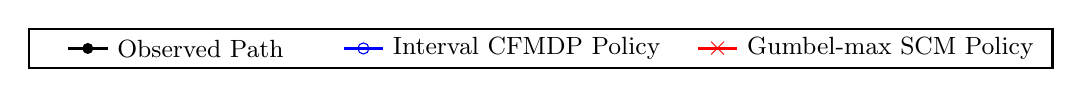
\begin{tikzpicture}[scale=1.0, every node/.style={scale=1.0}]
            \draw[thick, black] (-3, -0.25) rectangle (10, 0.25);
            %
            \draw[black, line width=1pt] (-2.5, 0.0) -- (-2,0.0);
            \fill[black] (-2.25,0.0) circle (2pt); %
            \node[right] at (-2,0.0) {\small Observed Path};
            
            %
            \draw[blue, line width=1pt] (1.0,0.0) -- (1.5,0.0);
            \node[draw=blue, circle, minimum size=4pt, inner sep=0pt] at (1.25,0.0) {}; %
            \node[right] at (1.5,0.0) {\small Interval CFMDP Policy};
            
            %
            \draw[red, line width=1pt] (5.5,0) -- (6,0);
            \node[red] at (5.75,0) {$\boldsymbol{\times}$}; %
            \node[right] at (6,0) {\small Gumbel-max SCM Policy};
        \end{tikzpicture}
    }\\
    %
    \subfigure[\footnotesize Lowest cumulative reward: Interval CFMDP ($312$), Gumbel-max SCM ($312$)]{%
        \resizebox{0.76\columnwidth}{!}{
             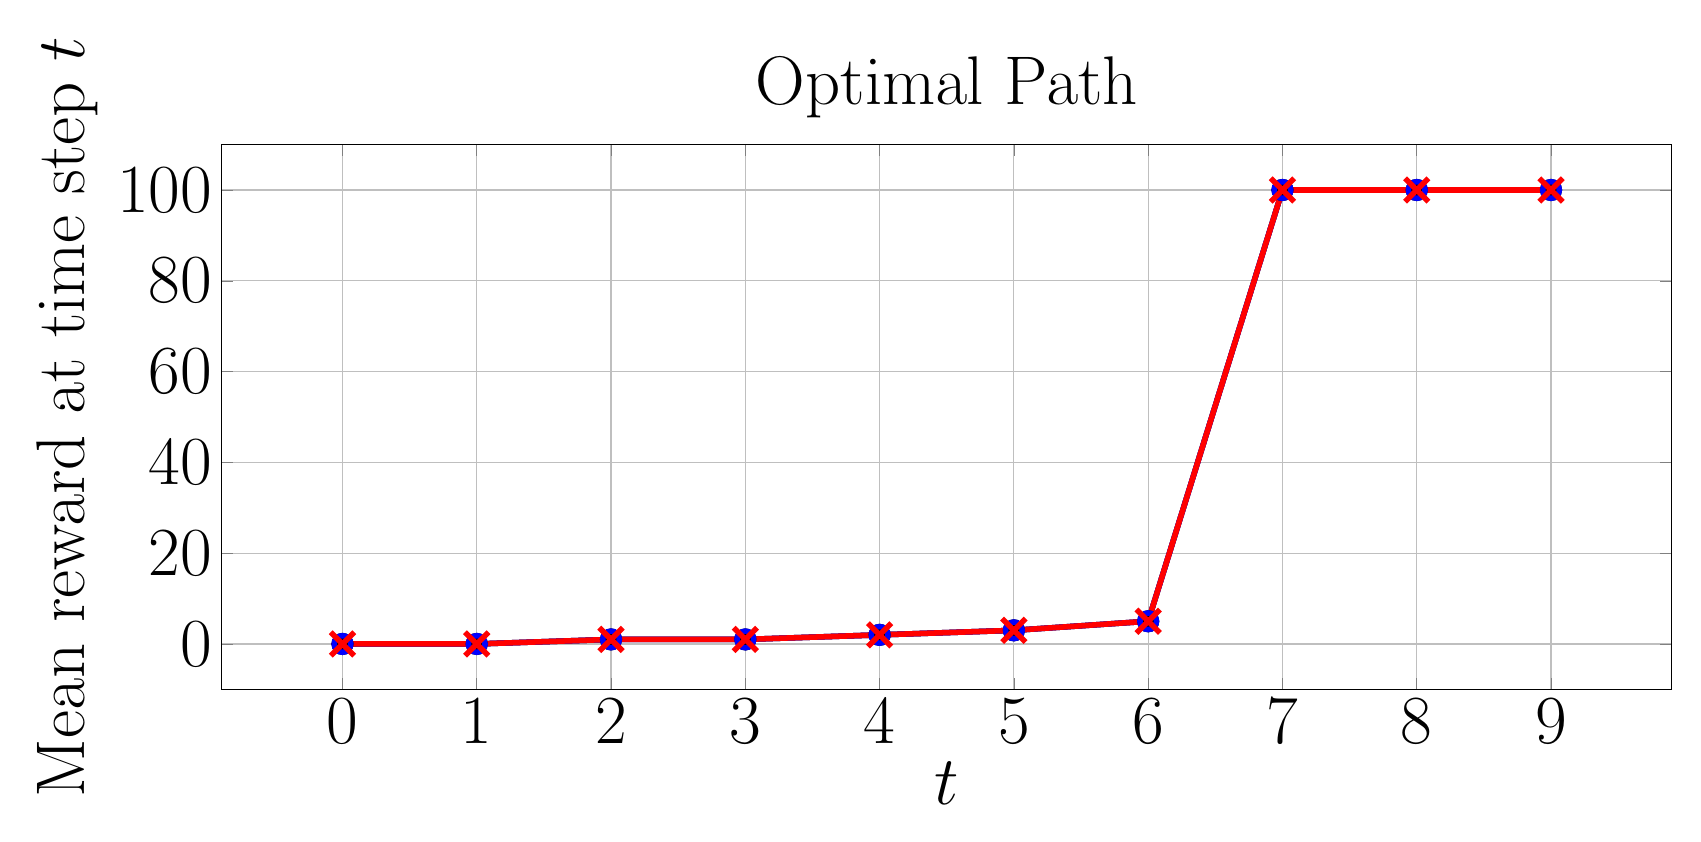
\begin{tikzpicture}
                \begin{axis}[
                    xlabel={$t$},
                    ylabel={Mean reward at time step $t$},
                    title={Optimal Path},
                    grid=both,
                    width=20cm, height=8.5cm,
                    every axis/.style={font=\Huge},
                    %
                ]
                \addplot[
                    color=black, %
                    mark=*, %
                    line width=2pt,
                    mark size=3pt,
                    error bars/.cd,
                    y dir=both, %
                    y explicit, %
                    error bar style={line width=1pt,solid},
                    error mark options={line width=1pt,mark size=4pt,rotate=90}
                ]
                coordinates {
                    (0, 0.0)  +- (0, 0.0)
                    (1, 0.0)  +- (0, 0.0) 
                    (2, 1.0)  +- (0, 0.0) 
                    (3, 1.0)  +- (0, 0.0)
                    (4, 2.0)  +- (0, 0.0)
                    (5, 3.0) +- (0, 0.0)
                    (6, 5.0) +- (0, 0.0)
                    (7, 100.0) +- (0, 0.0)
                    (8, 100.0) +- (0, 0.0)
                    (9, 100.0) +- (0, 0.0)
                };
                %
                \addplot[
                    color=blue, %
                    mark=o, %
                    line width=2pt,
                    mark size=3pt,
                    error bars/.cd,
                    y dir=both, %
                    y explicit, %
                    error bar style={line width=1pt,solid},
                    error mark options={line width=1pt,mark size=4pt,rotate=90}
                ]
                 coordinates {
                    (0, 0.0)  +- (0, 0.0)
                    (1, 0.0)  +- (0, 0.0) 
                    (2, 1.0)  +- (0, 0.0) 
                    (3, 1.0)  +- (0, 0.0)
                    (4, 2.0)  +- (0, 0.0)
                    (5, 3.0) +- (0, 0.0)
                    (6, 5.0) +- (0, 0.0)
                    (7, 100.0) +- (0, 0.0)
                    (8, 100.0) +- (0, 0.0)
                    (9, 100.0) +- (0, 0.0)
                };
                %
                \addplot[
                    color=red, %
                    mark=x, %
                    line width=2pt,
                    mark size=6pt,
                    error bars/.cd,
                    y dir=both, %
                    y explicit, %
                    error bar style={line width=1pt,solid},
                    error mark options={line width=1pt,mark size=4pt,rotate=90}
                ]
                coordinates {
                    (0, 0.0)  +- (0, 0.0)
                    (1, 0.0)  +- (0, 0.0) 
                    (2, 1.0)  +- (0, 0.0) 
                    (3, 1.0)  +- (0, 0.0)
                    (4, 2.0)  +- (0, 0.0)
                    (5, 3.0) +- (0, 0.0)
                    (6, 5.0) +- (0, 0.0)
                    (7, 100.0) +- (0, 0.0)
                    (8, 100.0) +- (0, 0.0)
                    (9, 100.0) +- (0, 0.0)
                };
                \end{axis}
            \end{tikzpicture}
         }
    }
    \hspace{1cm}
    \subfigure[\footnotesize Lowest cumulative reward: Interval CFMDP ($19$), Gumbel-max SCM ($-88$)]{%
         \resizebox{0.76\columnwidth}{!}{
            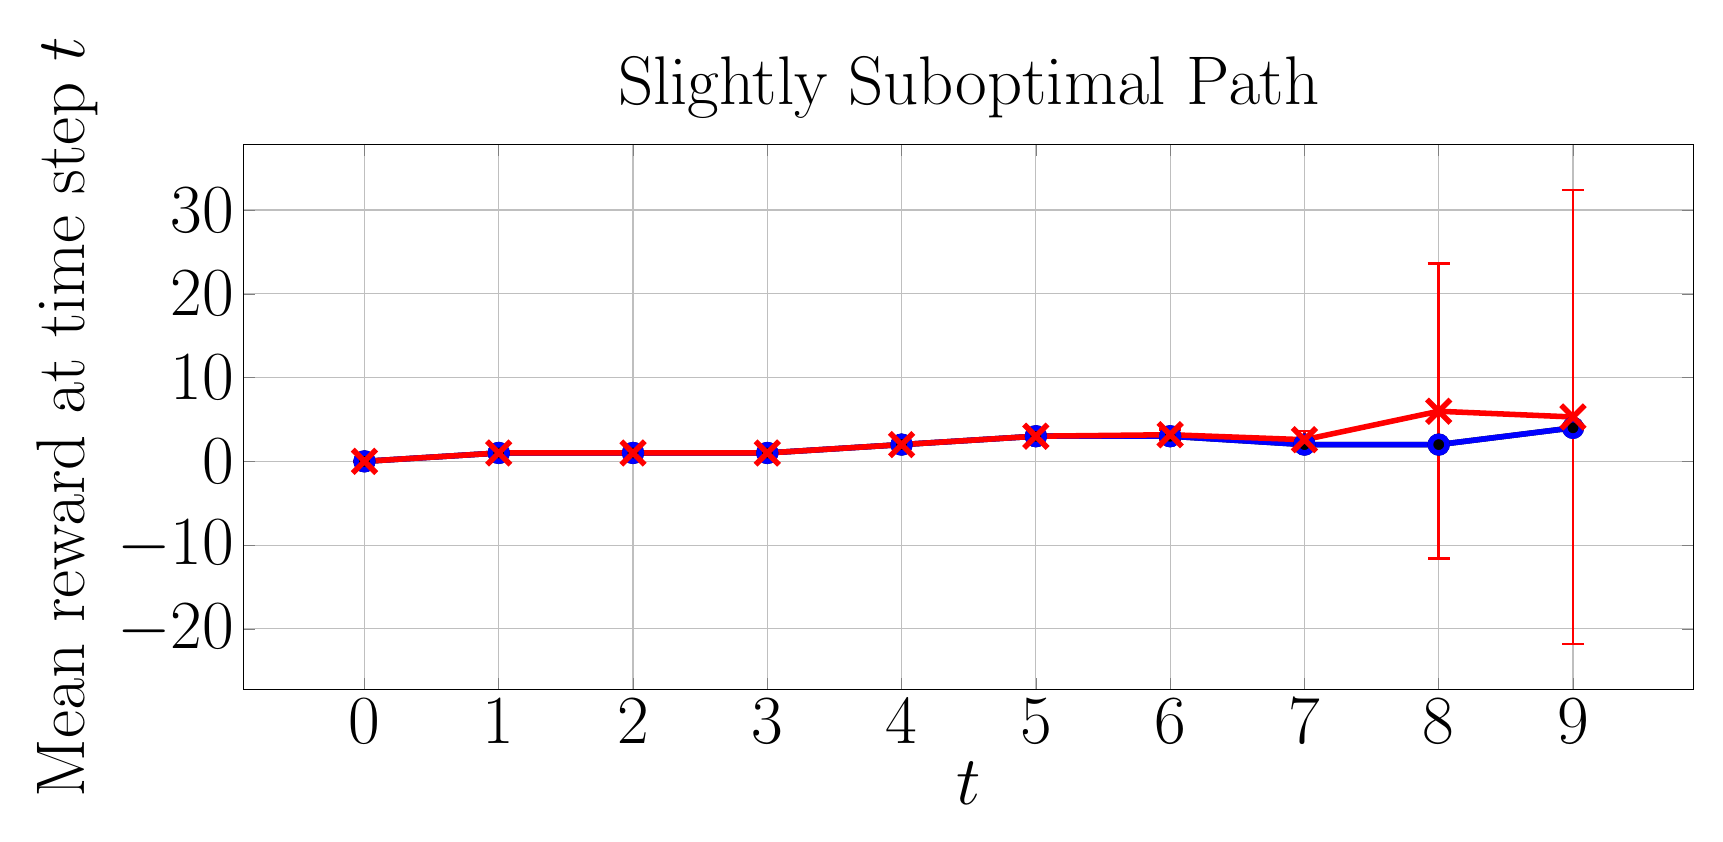
\begin{tikzpicture}
                \begin{axis}[
                    xlabel={$t$},
                    ylabel={Mean reward at time step $t$},
                    title={Slightly Suboptimal Path},
                    grid=both,
                    width=20cm, height=8.5cm,
                    every axis/.style={font=\Huge},
                    %
                ]
                \addplot[
                    color=black, %
                    mark=*, %
                    line width=2pt,
                    mark size=3pt,
                    error bars/.cd,
                    y dir=both, %
                    y explicit, %
                    error bar style={line width=1pt,solid},
                    error mark options={line width=1pt,mark size=4pt,rotate=90}
                ]
              coordinates {
                    (0, 0.0)  +- (0, 0.0)
                    (1, 1.0)  +- (0, 0.0) 
                    (2, 1.0)  +- (0, 0.0) 
                    (3, 1.0)  +- (0, 0.0)
                    (4, 2.0)  +- (0, 0.0)
                    (5, 3.0) +- (0, 0.0)
                    (6, 3.0) +- (0, 0.0)
                    (7, 2.0) +- (0, 0.0)
                    (8, 2.0) +- (0, 0.0)
                    (9, 4.0) +- (0, 0.0)
                };
                %
                \addplot[
                    color=blue, %
                    mark=o, %
                    line width=2pt,
                    mark size=3pt,
                    error bars/.cd,
                    y dir=both, %
                    y explicit, %
                    error bar style={line width=1pt,solid},
                    error mark options={line width=1pt,mark size=4pt,rotate=90}
                ]
              coordinates {
                    (0, 0.0)  +- (0, 0.0)
                    (1, 1.0)  +- (0, 0.0) 
                    (2, 1.0)  +- (0, 0.0) 
                    (3, 1.0)  +- (0, 0.0)
                    (4, 2.0)  +- (0, 0.0)
                    (5, 3.0) +- (0, 0.0)
                    (6, 3.0) +- (0, 0.0)
                    (7, 2.0) +- (0, 0.0)
                    (8, 2.0) +- (0, 0.0)
                    (9, 4.0) +- (0, 0.0)
                };
                %
                \addplot[
                    color=red, %
                    mark=x, %
                    line width=2pt,
                    mark size=6pt,
                    error bars/.cd,
                    y dir=both, %
                    y explicit, %
                    error bar style={line width=1pt,solid},
                    error mark options={line width=1pt,mark size=4pt,rotate=90}
                ]
                coordinates {
                    (0, 0.0)  +- (0, 0.0)
                    (1, 1.0)  +- (0, 0.0) 
                    (2, 1.0)  +- (0, 0.0) 
                    (3, 1.0)  +- (0, 0.0)
                    (4, 2.0)  += (0, 0.0)
                    (5, 3.0)  += (0, 0.0)
                    (6, 3.17847) += (0, 0.62606746) -= (0, 0.62606746)
                    (7, 2.5832885) += (0, 1.04598233) -= (0, 1.04598233)
                    (8, 5.978909) += (0, 17.60137623) -= (0, 17.60137623)
                    (9, 5.297059) += (0, 27.09227512) -= (0, 27.09227512)
                };
                \end{axis}
            \end{tikzpicture}
         }
    }\\[-1.5pt]
    \subfigure[\footnotesize Lowest cumulative reward: Interval CFMDP ($14$), Gumbel-max SCM ($-598$)]{%
         \resizebox{0.76\columnwidth}{!}{
             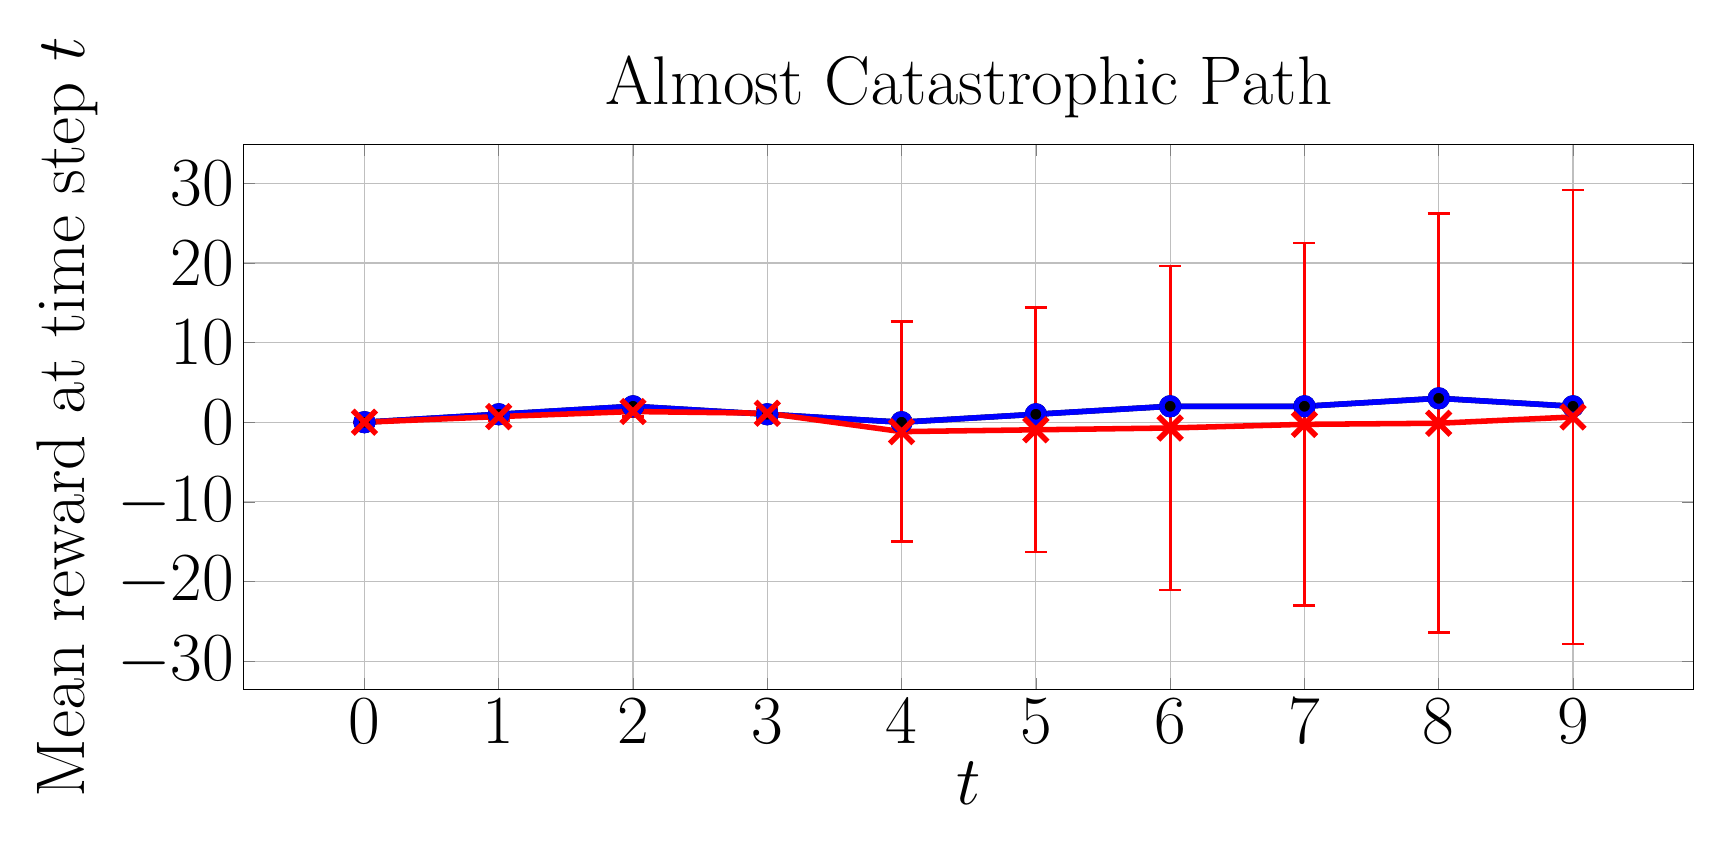
\begin{tikzpicture}
                \begin{axis}[
                    xlabel={$t$},
                    ylabel={Mean reward at time step $t$},
                    title={Almost Catastrophic Path},
                    grid=both,
                    width=20cm, height=8.5cm,
                    every axis/.style={font=\Huge},
                    %
                ]
                \addplot[
                    color=black, %
                    mark=*, %
                    line width=2pt,
                    mark size=3pt,
                    error bars/.cd,
                    y dir=both, %
                    y explicit, %
                    error bar style={line width=1pt,solid},
                    error mark options={line width=1pt,mark size=4pt,rotate=90}
                ]
                coordinates {
                    (0, 0.0)  +- (0, 0.0)
                    (1, 1.0)  +- (0, 0.0) 
                    (2, 2.0)  +- (0, 0.0) 
                    (3, 1.0)  +- (0, 0.0)
                    (4, 0.0)  +- (0, 0.0)
                    (5, 1.0) +- (0, 0.0)
                    (6, 2.0) +- (0, 0.0)
                    (7, 2.0) +- (0, 0.0)
                    (8, 3.0) +- (0, 0.0)
                    (9, 2.0) +- (0, 0.0)
                };
                %
                \addplot[
                    color=blue, %
                    mark=o, %
                    line width=2pt,
                    mark size=3pt,
                    error bars/.cd,
                    y dir=both, %
                    y explicit, %
                    error bar style={line width=1pt,solid},
                    error mark options={line width=1pt,mark size=4pt,rotate=90}
                ]
                coordinates {
                    (0, 0.0)  +- (0, 0.0)
                    (1, 1.0)  +- (0, 0.0) 
                    (2, 2.0)  +- (0, 0.0) 
                    (3, 1.0)  +- (0, 0.0)
                    (4, 0.0)  +- (0, 0.0)
                    (5, 1.0) +- (0, 0.0)
                    (6, 2.0) +- (0, 0.0)
                    (7, 2.0) +- (0, 0.0)
                    (8, 3.0) +- (0, 0.0)
                    (9, 2.0) +- (0, 0.0)
                };
                %
                \addplot[
                    color=red, %
                    mark=x, %
                    line width=2pt,
                    mark size=6pt,
                    error bars/.cd,
                    y dir=both, %
                    y explicit, %
                    error bar style={line width=1pt,solid},
                    error mark options={line width=1pt,mark size=4pt,rotate=90}
                ]
                coordinates {
                    (0, 0.0)  +- (0, 0.0)
                    (1, 0.7065655)  +- (0, 0.4553358) 
                    (2, 1.341673)  +- (0, 0.67091621) 
                    (3, 1.122926)  +- (0, 0.61281824)
                    (4, -1.1821935)  +- (0, 13.82444042)
                    (5, -0.952399)  +- (0, 15.35195457)
                    (6, -0.72672) +- (0, 20.33508414)
                    (7, -0.268983) +- (0, 22.77861454)
                    (8, -0.1310835) +- (0, 26.31013314)
                    (9, 0.65806) +- (0, 28.50670214)
                };
                %
            %
            %
            %
            %
            %
            %
            %
            %
            %
            %
            %
            %
            %
            %
            %
            %
            %
            %
                \end{axis}
            \end{tikzpicture}
         }
    }
    \hspace{1cm}
    \subfigure[\footnotesize Lowest cumulative reward: Interval CFMDP ($-698$), Gumbel-max SCM ($-698$)]{%
         \resizebox{0.76\columnwidth}{!}{
            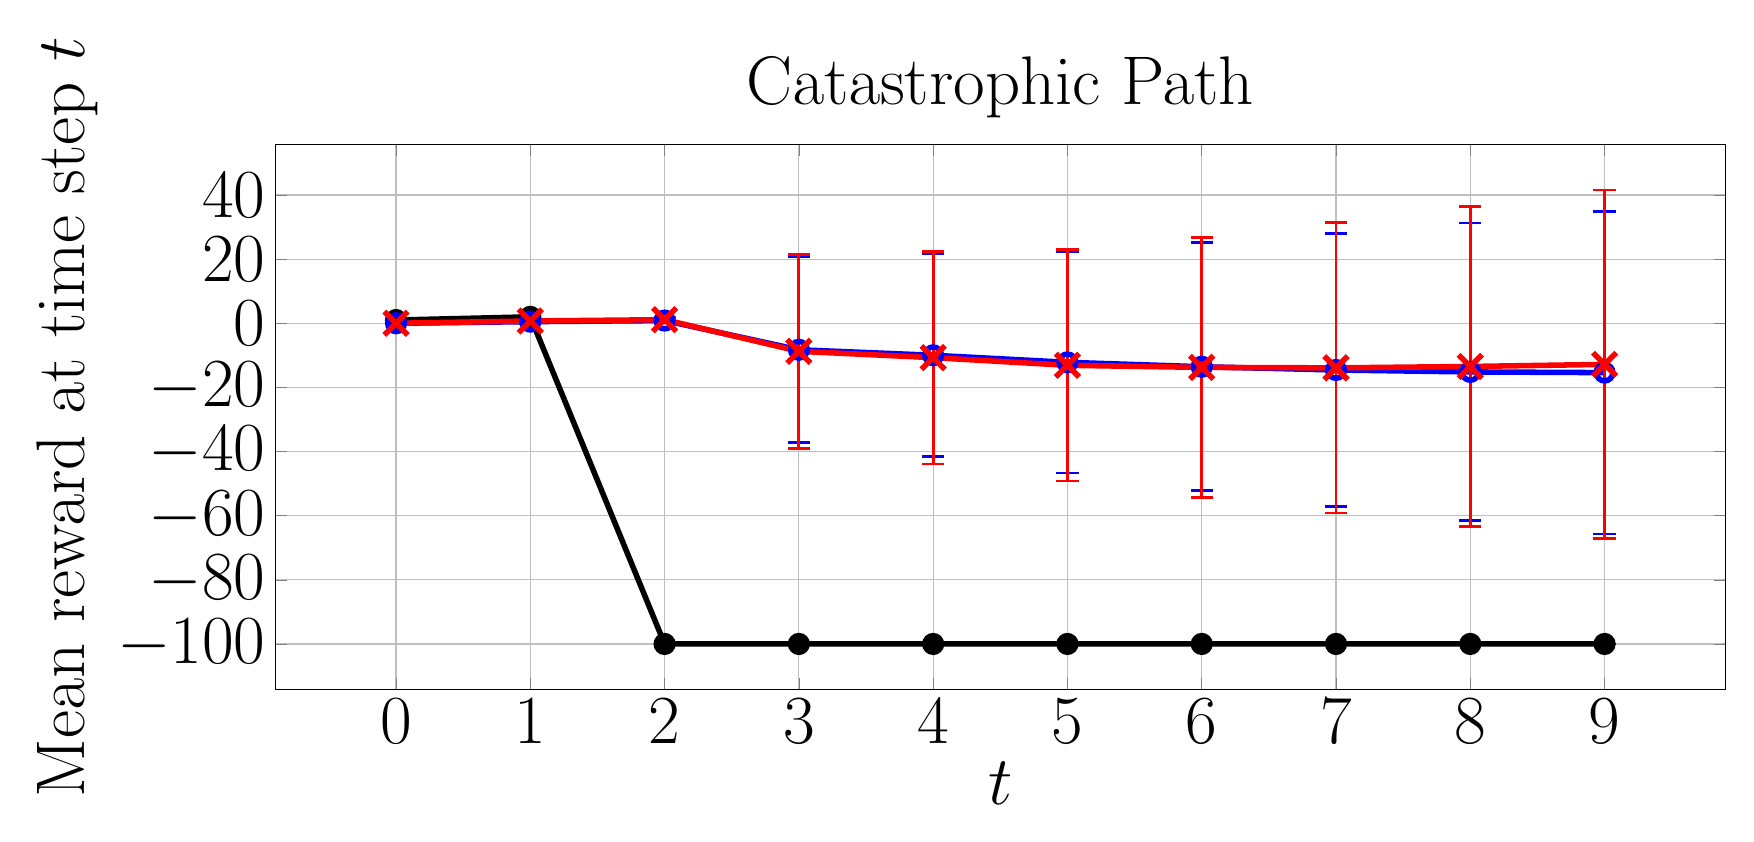
\begin{tikzpicture}
                \begin{axis}[
                    xlabel={$t$},
                    ylabel={Mean reward at time step $t$},
                    title={Catastrophic Path},
                    grid=both,
                    width=20cm, height=8.5cm,
                    every axis/.style={font=\Huge},
                    %
                ]
                \addplot[
                    color=black, %
                    mark=*, %
                    line width=2pt,
                    mark size=3pt,
                    error bars/.cd,
                    y dir=both, %
                    y explicit, %
                    error bar style={line width=1pt,solid},
                    error mark options={line width=1pt,mark size=4pt,rotate=90}
                ]
                coordinates {
                    (0, 1.0)  +- (0, 0.0)
                    (1, 2.0)  +- (0, 0.0) 
                    (2, -100.0)  +- (0, 0.0) 
                    (3, -100.0)  +- (0, 0.0)
                    (4, -100.0)  +- (0, 0.0)
                    (5, -100.0) +- (0, 0.0)
                    (6, -100.0) +- (0, 0.0)
                    (7, -100.0) +- (0, 0.0)
                    (8, -100.0) +- (0, 0.0)
                    (9, -100.0) +- (0, 0.0)
                };
                %
                \addplot[
                    color=blue, %
                    mark=o, %
                    line width=2pt,
                    mark size=3pt,
                    error bars/.cd,
                    y dir=both, %
                    y explicit, %
                    error bar style={line width=1pt,solid},
                    error mark options={line width=1pt,mark size=4pt,rotate=90}
                ]
                coordinates {
                    (0, 0.0)  +- (0, 0.0)
                    (1, 0.504814)  +- (0, 0.49997682) 
                    (2, 0.8439835)  +- (0, 0.76831917) 
                    (3, -8.2709165)  +- (0, 28.93656754)
                    (4, -9.981082)  +- (0, 31.66825363)
                    (5, -12.1776325) +- (0, 34.53463233)
                    (6, -13.556076) +- (0, 38.62845372)
                    (7, -14.574418) +- (0, 42.49603359)
                    (8, -15.1757075) +- (0, 46.41913968)
                    (9, -15.3900395) +- (0, 50.33563368)
                };
                %
                \addplot[
                    color=red, %
                    mark=x, %
                    line width=2pt,
                    mark size=6pt,
                    error bars/.cd,
                    y dir=both, %
                    y explicit, %
                    error bar style={line width=1pt,solid},
                    error mark options={line width=1pt,mark size=4pt,rotate=90}
                ]
                coordinates {
                    (0, 0.0)  +- (0, 0.0)
                    (1, 0.701873)  +- (0, 0.45743556) 
                    (2, 1.1227805)  +- (0, 0.73433129) 
                    (3, -8.7503255)  +- (0, 30.30257976)
                    (4, -10.722092)  +- (0, 33.17618589)
                    (5, -13.10721)  +- (0, 36.0648089)
                    (6, -13.7631645) +- (0, 40.56553451)
                    (7, -13.909043) +- (0, 45.23829402)
                    (8, -13.472517) +- (0, 49.96270296)
                    (9, -12.8278835) +- (0, 54.38618735)
                };
                %
            %
            %
            %
            %
            %
            %
            %
            %
            %
            %
            %
            %
            %
            %
            %
            %
            %
            %
                \end{axis}
            \end{tikzpicture}
         }
    }
    \caption{Average instant reward of CF paths induced by policies on GridWorld $p=0.4$.}
    \label{fig: reward p=0.4}
\end{figure*}

\subsection{Experimental Setup}
To compare policy performance, we measure the average rewards of counterfactual paths induced by our policy and the Gumbel-max policy by uniformly sampling $200$ counterfactual MDPs from the ICFMDP and generating $10,000$ counterfactual paths over each sampled CFMDP. \jl{Since the interval CFMDP depends on the observed path, we select $4$  paths of varying optimality to evaluate how the observed path impacts the performance of both policies: an optimal path, a slightly suboptimal path that could reach the optimal reward with a few changes, a catastrophic path that enters a catastrophic, terminal state with low reward, and an almost catastrophic path that was close to entering a catastrophic state.} When measuring the average probability bound widths and execution time needed to generate the ICFMDPs, we averaged over $20$ randomly generated observed paths
\footnote{Further training details are provided in Appendix \ref{app: training details}, and the code is provided at \href{https://github.com/ddv-lab/robust-cf-inference-in-MDPs}{https://github.com/ddv-lab/robust-cf-inference-in-MDPs}
%
%
.}.

\subsection{GridWorld}
\jl{The GridWorld MDP is a $4 \times 4$ grid where an agent must navigate from the top-left corner to the goal state in the bottom-right corner, avoiding a dangerous terminal state in the centre. At each time step, the agent can move up, down, left, or right, but there is a small probability (controlled by hyper-parameter $p$) of moving in an unintended direction. As the agent nears the goal, the reward for each state increases, culminating in a reward of $+100$ for reaching the goal. Entering the dangerous state results in a penalty of $-100$. We use two versions of GridWorld: a less stochastic version with $p=0.9$ (i.e., $90$\% chance of moving in the chosen direction) and a more stochastic version with $p=0.4$.}

\paragraph{GridWorld ($p=0.9$)}
When $p=0.9$, the counterfactual probability bounds are typically narrow (see Table \ref{tab:nonzero_probs} for average measurements). Consequently, as shown in Figure \ref{fig: reward p=0.9}, both policies are nearly identical and perform similarly well across the optimal, slightly suboptimal, and catastrophic paths.
%
However, for the almost catastrophic path, the interval CFMDP path is more conservative and follows the observed path more closely (as this is where the probability bounds are narrowest), which typically requires one additional step to reach the goal state than the Gumbel-max SCM policy.
%

\paragraph{GridWorld ($p=0.4$)}
\jl{When $p=0.4$, the GridWorld environment becomes more uncertain, increasing the risk of entering the dangerous state even if correct actions are chosen. Thus, as shown in Figure \ref{fig: reward p=0.4}, the interval CFMDP policy adopts a more conservative approach, avoiding deviation from the observed policy if it cannot guarantee higher counterfactual rewards (see the slightly suboptimal and almost catastrophic paths), whereas the Gumbel-max SCM is inconsistent: it can yield higher rewards, but also much lower rewards, reflected in the wide error bars.} For the catastrophic path, both policies must deviate from the observed path to achieve a higher reward and, in this case, perform similarly.
%
%
%
%
\subsection{Sepsis}
The Sepsis MDP \citep{oberst2019counterfactual} simulates trajectories of Sepsis patients. Each state consists of four vital signs (heart rate, blood pressure, oxygen concentration, and glucose levels), categorised as low, normal, or high.
and three treatments that can be toggled on/off at each time step (8 actions in total). Unlike \citet{oberst2019counterfactual}, we scale rewards based on the number of out-of-range vital signs, between $-1000$ (patient dies) and $1000$ (patient discharged). \jl{Like the GridWorld $p=0.4$ experiment, the Sepsis MDP is highly uncertain, as many states are equally likely to lead to optimal and poor outcomes. Thus, as shown in Figure \ref{fig: reward sepsis}, both policies follow the observed optimal and almost catastrophic paths to guarantee rewards are no worse than the observation.} However, improving the catastrophic path requires deviating from the observation. Here, the Gumbel-max SCM policy, on average, performs better than the interval CFMDP policy. But, since both policies have lower bounds clipped at $-1000$, neither policy reliably improves over the observation. In contrast, for the slightly suboptimal path, the interval CFMDP policy performs significantly better, shown by its higher lower bounds. 
Moreover, in these two cases, the worst-case counterfactual path generated by the interval CFMDP policy is better than that of the Gumbel-max SCM policy,
indicating its greater robustness.
%
\begin{figure*}
    \centering
     \resizebox{0.6\textwidth}{!}{
        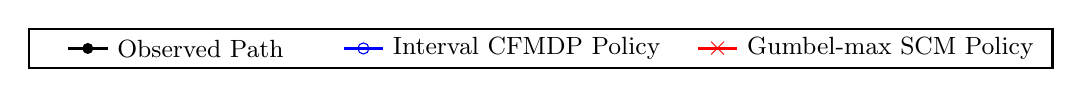
\begin{tikzpicture}[scale=1.0, every node/.style={scale=1.0}]
            \draw[thick, black] (-3, -0.25) rectangle (10, 0.25);
            %
            \draw[black, line width=1pt] (-2.5, 0.0) -- (-2,0.0);
            \fill[black] (-2.25,0.0) circle (2pt); %
            \node[right] at (-2,0.0) {\small Observed Path};
            
            %
            \draw[blue, line width=1pt] (1.0,0.0) -- (1.5,0.0);
            \node[draw=blue, circle, minimum size=4pt, inner sep=0pt] at (1.25,0.0) {}; %
            \node[right] at (1.5,0.0) {\small Interval CFMDP Policy};
            
            %
            \draw[red, line width=1pt] (5.5,0) -- (6,0);
            \node[red] at (5.75,0) {$\boldsymbol{\times}$}; %
            \node[right] at (6,0) {\small Gumbel-max SCM Policy};
        \end{tikzpicture}
    }\\
    \subfigure[\footnotesize Lowest cumulative reward: Interval CFMDP ($8000$), Gumbel-max SCM ($8000$)]{%
         \resizebox{0.76\columnwidth}{!}{
             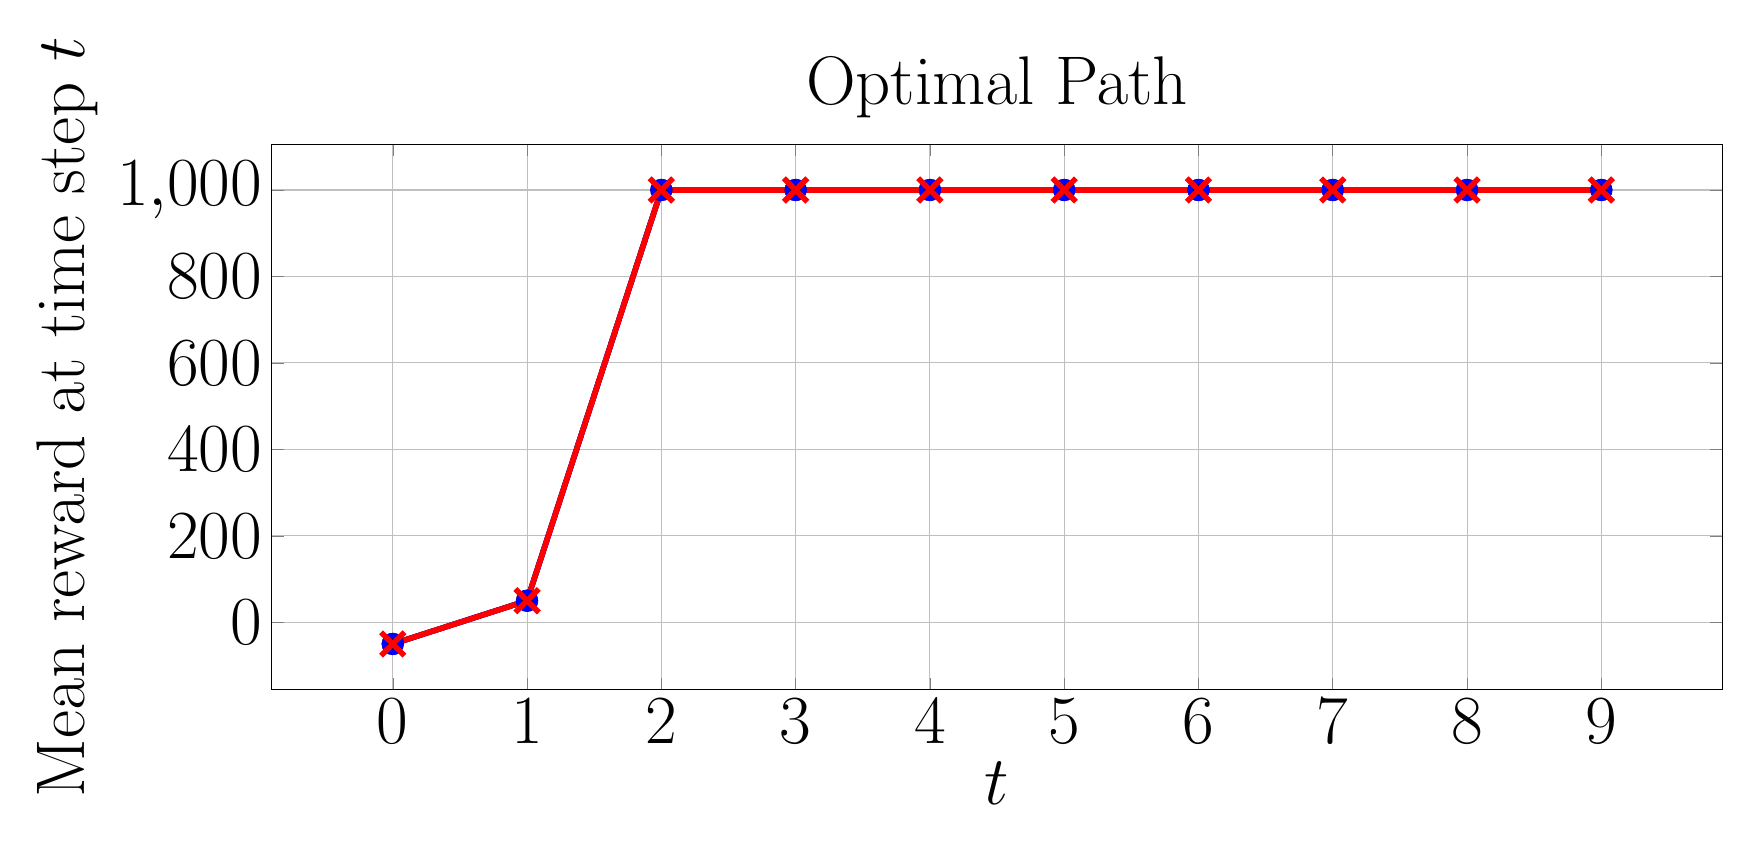
\begin{tikzpicture}
                \begin{axis}[
                    xlabel={$t$},
                    ylabel={Mean reward at time step $t$},
                    title={Optimal Path},
                    grid=both,
                    width=20cm, height=8.5cm,
                    every axis/.style={font=\Huge},
                    %
                ]
                \addplot[
                    color=black, %
                    mark=*, %
                    line width=2pt,
                    mark size=3pt,
                ]
                coordinates {
                    (0, -50.0)
                    (1, 50.0)
                    (2, 1000.0)
                    (3, 1000.0)
                    (4, 1000.0)
                    (5, 1000.0)
                    (6, 1000.0)
                    (7, 1000.0)
                    (8, 1000.0)
                    (9, 1000.0)
                };
                %
                \addplot[
                    color=blue, %
                    mark=o, %
                    line width=2pt,
                    mark size=3pt,
                    error bars/.cd,
                    y dir=both, %
                    y explicit, %
                    error bar style={line width=1pt,solid},
                    error mark options={line width=1pt,mark size=4pt,rotate=90}
                ]
                coordinates {
                    (0, -50.0)  +- (0, 0.0)
                    (1, 50.0)  +- (0, 0.0) 
                    (2, 1000.0)  +- (0, 0.0) 
                    (3, 1000.0)  +- (0, 0.0)
                    (4, 1000.0)  +- (0, 0.0)
                    (5, 1000.0) +- (0, 0.0)
                    (6, 1000.0) +- (0, 0.0)
                    (7, 1000.0) +- (0, 0.0)
                    (8, 1000.0) +- (0, 0.0)
                    (9, 1000.0) +- (0, 0.0)
                };
                %
                \addplot[
                    color=red, %
                    mark=x, %
                    line width=2pt,
                    mark size=6pt,
                    error bars/.cd,
                    y dir=both, %
                    y explicit, %
                    error bar style={line width=1pt,solid},
                    error mark options={line width=1pt,mark size=4pt,rotate=90}
                ]
                coordinates {
                    (0, -50.0)  +- (0, 0.0)
                    (1, 50.0)  +- (0, 0.0) 
                    (2, 1000.0)  +- (0, 0.0) 
                    (3, 1000.0)  +- (0, 0.0)
                    (4, 1000.0)  +- (0, 0.0)
                    (5, 1000.0) +- (0, 0.0)
                    (6, 1000.0) +- (0, 0.0)
                    (7, 1000.0) +- (0, 0.0)
                    (8, 1000.0) +- (0, 0.0)
                    (9, 1000.0) +- (0, 0.0)
                };
                %
                \end{axis}
            \end{tikzpicture}
         }
    }
    \hspace{1cm}
    \subfigure[\footnotesize Lowest cumulative reward: Interval CFMDP ($-5980$), Gumbel-max SCM ($-8000$)]{%
         \resizebox{0.76\columnwidth}{!}{
            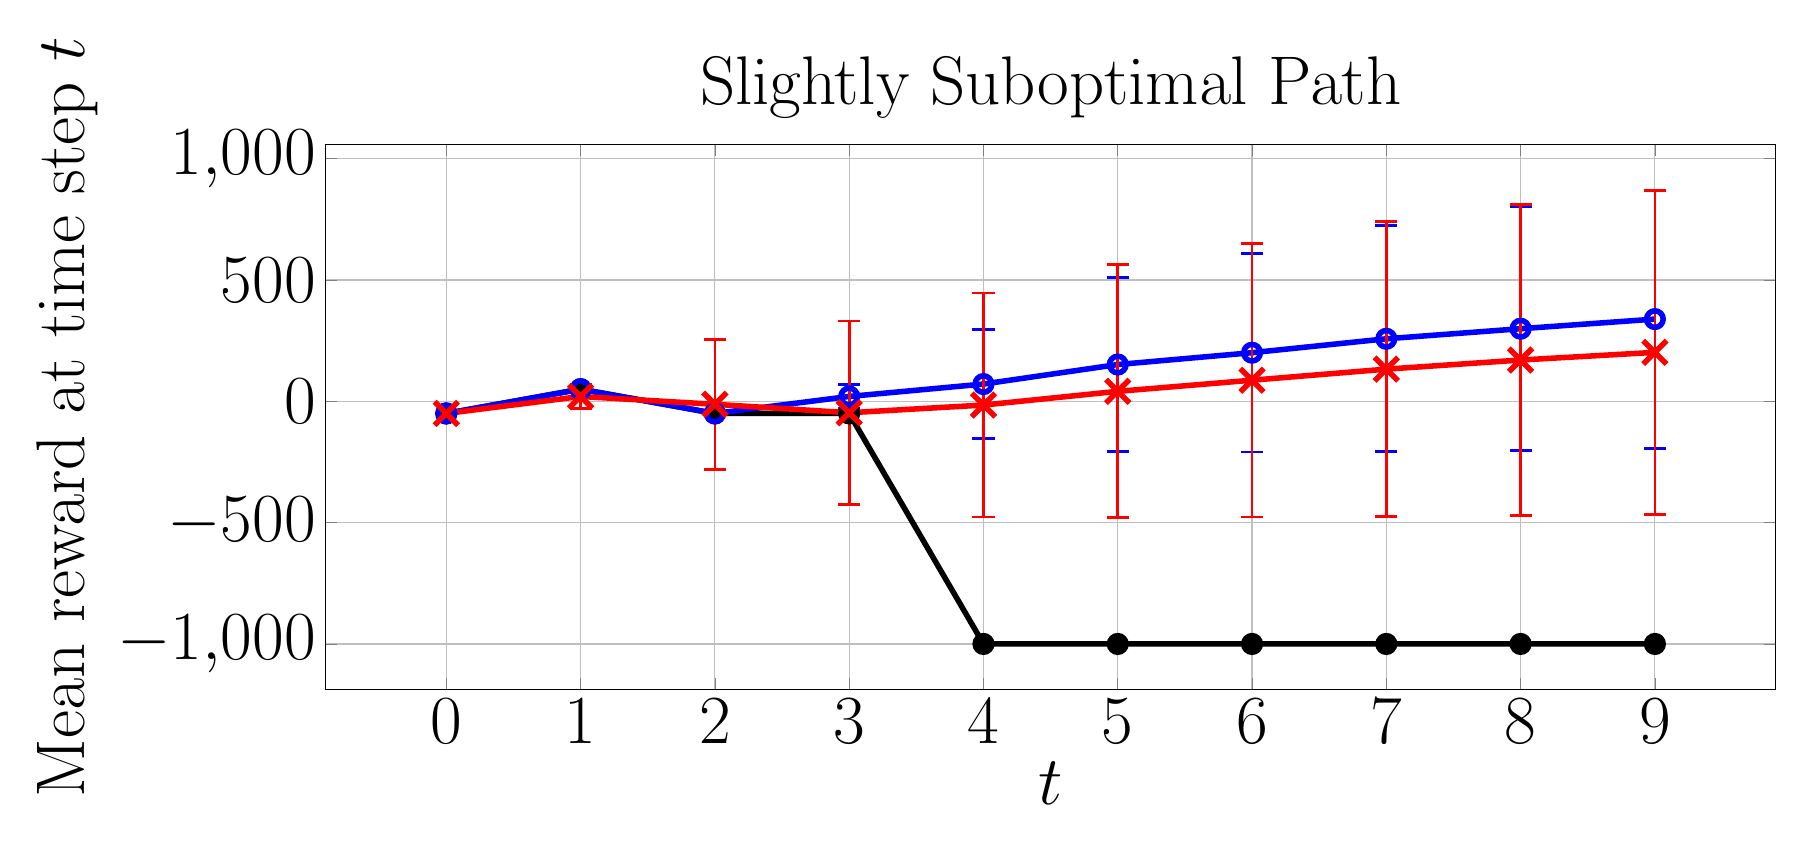
\begin{tikzpicture}
                \begin{axis}[
                    xlabel={$t$},
                    ylabel={Mean reward at time step $t$},
                    title={Slightly Suboptimal Path},
                    grid=both,
                    width=20cm, height=8.5cm,
                    every axis/.style={font=\Huge},
                    %
                ]
               \addplot[
                    color=black, %
                    mark=*, %
                    line width=2pt,
                    mark size=3pt,
                ]
                coordinates {
                    (0, -50.0)
                    (1, 50.0)
                    (2, -50.0)
                    (3, -50.0)
                    (4, -1000.0)
                    (5, -1000.0)
                    (6, -1000.0)
                    (7, -1000.0)
                    (8, -1000.0)
                    (9, -1000.0)
                };
                %
                \addplot[
                    color=blue, %
                    mark=o, %
                    line width=2pt,
                    mark size=3pt,
                    error bars/.cd,
                    y dir=both, %
                    y explicit, %
                    error bar style={line width=1pt,solid},
                    error mark options={line width=1pt,mark size=4pt,rotate=90}
                ]
                coordinates {
                    (0, -50.0)  +- (0, 0.0)
                    (1, 50.0)  +- (0, 0.0) 
                    (2, -50.0)  +- (0, 0.0) 
                    (3, 20.0631)  +- (0, 49.97539413)
                    (4, 71.206585)  +- (0, 226.02033693)
                    (5, 151.60797) +- (0, 359.23292559)
                    (6, 200.40593) +- (0, 408.86185176)
                    (7, 257.77948) +- (0, 466.10372804)
                    (8, 299.237465) +- (0, 501.82579506)
                    (9, 338.9129) +- (0, 532.06124996)
                };
                %
                \addplot[
                    color=red, %
                    mark=x, %
                    line width=2pt,
                    mark size=6pt,
                    error bars/.cd,
                    y dir=both, %
                    y explicit, %
                    error bar style={line width=1pt,solid},
                    error mark options={line width=1pt,mark size=4pt,rotate=90}
                ]
                coordinates {
                    (0, -50.0)  +- (0, 0.0)
                    (1, 20.00736)  +- (0, 49.99786741) 
                    (2, -12.282865)  +- (0, 267.598755) 
                    (3, -47.125995)  +- (0, 378.41755832)
                    (4, -15.381965)  +- (0, 461.77616558)
                    (5, 41.15459) +- (0, 521.53189262)
                    (6, 87.01595) +- (0, 564.22243126 )
                    (7, 132.62376) +- (0, 607.31338037)
                    (8, 170.168145) +- (0, 641.48013693)
                    (9, 201.813135) +- (0, 667.29441777)
                };
                %
                %
                %
                %
                %
                %
                %
                %
                %
                %
                %
                %
                %
                %
                %
                %
                %
                %
                %
                \end{axis}
            \end{tikzpicture}
         }
    }\\[-1.5pt]
    \subfigure[\footnotesize Lowest cumulative reward: Interval CFMDP ($100$), Gumbel-max SCM ($100$)]{%
         \resizebox{0.76\columnwidth}{!}{
             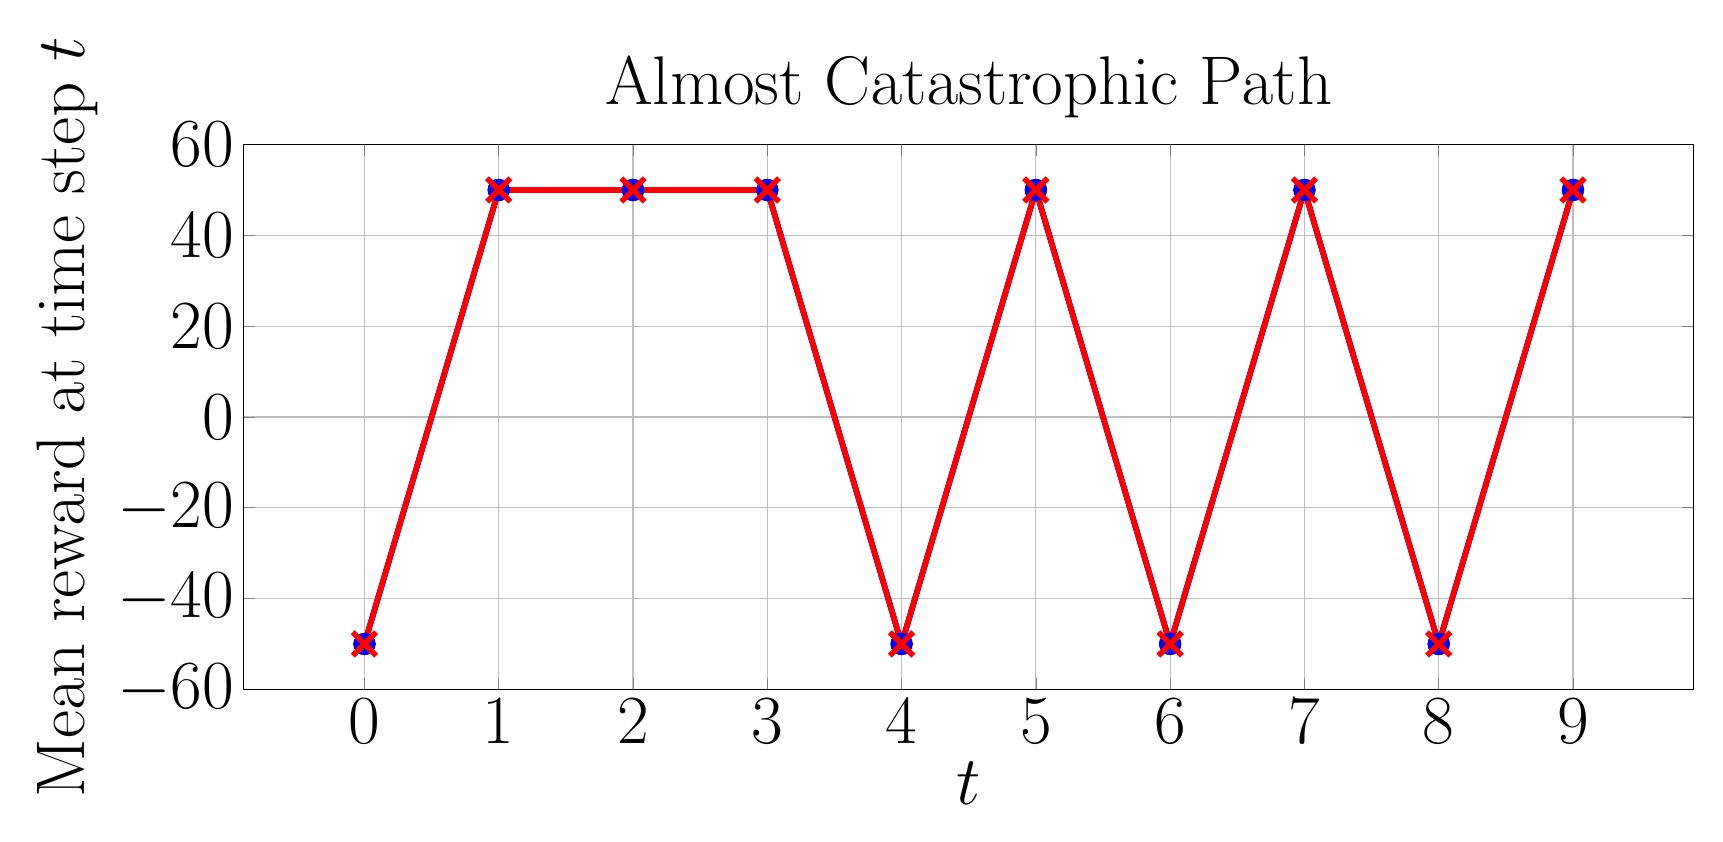
\begin{tikzpicture}
                \begin{axis}[
                    xlabel={$t$},
                    ylabel={Mean reward at time step $t$},
                    title={Almost Catastrophic Path},
                    grid=both,
                    every axis/.style={font=\Huge},
                    width=20cm, height=8.5cm,
                    %
                ]
               \addplot[
                    color=black, %
                    mark=*, %
                    line width=2pt,
                    mark size=3pt,
                ]
                coordinates {
                    (0, -50.0)
                    (1, 50.0)
                    (2, 50.0)
                    (3, 50.0)
                    (4, -50.0)
                    (5, 50.0)
                    (6, -50.0)
                    (7, 50.0)
                    (8, -50.0)
                    (9, 50.0)
                };
                %
                %
                \addplot[
                    color=blue, %
                    mark=o, %
                    line width=2pt,
                    mark size=3pt,
                    error bars/.cd,
                    y dir=both, %
                    y explicit, %
                    error bar style={line width=1pt,solid},
                    error mark options={line width=1pt,mark size=4pt,rotate=90}
                ]
                coordinates {
                    (0, -50.0)  +- (0, 0.0)
                    (1, 50.0)  +- (0, 0.0) 
                    (2, 50.0)  +- (0, 0.0) 
                    (3, 50.0)  +- (0, 0.0)
                    (4, -50.0)  +- (0, 0.0)
                    (5, 50.0) +- (0, 0.0)
                    (6, -50.0) +- (0, 0.0)
                    (7, 50.0) +- (0, 0.0)
                    (8, -50.0) +- (0, 0.0)
                    (9, 50.0) +- (0, 0.0)
                };
                %
                \addplot[
                    color=red, %
                    mark=x, %
                    line width=2pt,
                    mark size=6pt,
                    error bars/.cd,
                    y dir=both, %
                    y explicit, %
                    error bar style={line width=1pt,solid},
                    error mark options={line width=1pt,mark size=4pt,rotate=90}
                ]
                coordinates {
                    (0, -50.0)  +- (0, 0.0)
                    (1, 50.0)  +- (0, 0.0) 
                    (2, 50.0)  +- (0, 0.0) 
                    (3, 50.0)  +- (0, 0.0)
                    (4, -50.0)  +- (0, 0.0)
                    (5, 50.0) +- (0, 0.0)
                    (6, -50.0) +- (0, 0.0)
                    (7, 50.0) +- (0, 0.0)
                    (8, -50.0) +- (0, 0.0)
                    (9, 50.0) +- (0, 0.0)
                };
                %
                %
                %
                %
                %
                %
                %
                %
                %
                %
                %
                %
                %
                %
                %
                %
                %
                %
                %
                \end{axis}
            \end{tikzpicture}
         }
    }
    \hspace{1cm}
    \subfigure[\footnotesize Lowest cumulative reward: Interval CFMDP ($-7150$), Gumbel-max SCM ($-9050$)]{%
         \resizebox{0.76\columnwidth}{!}{
            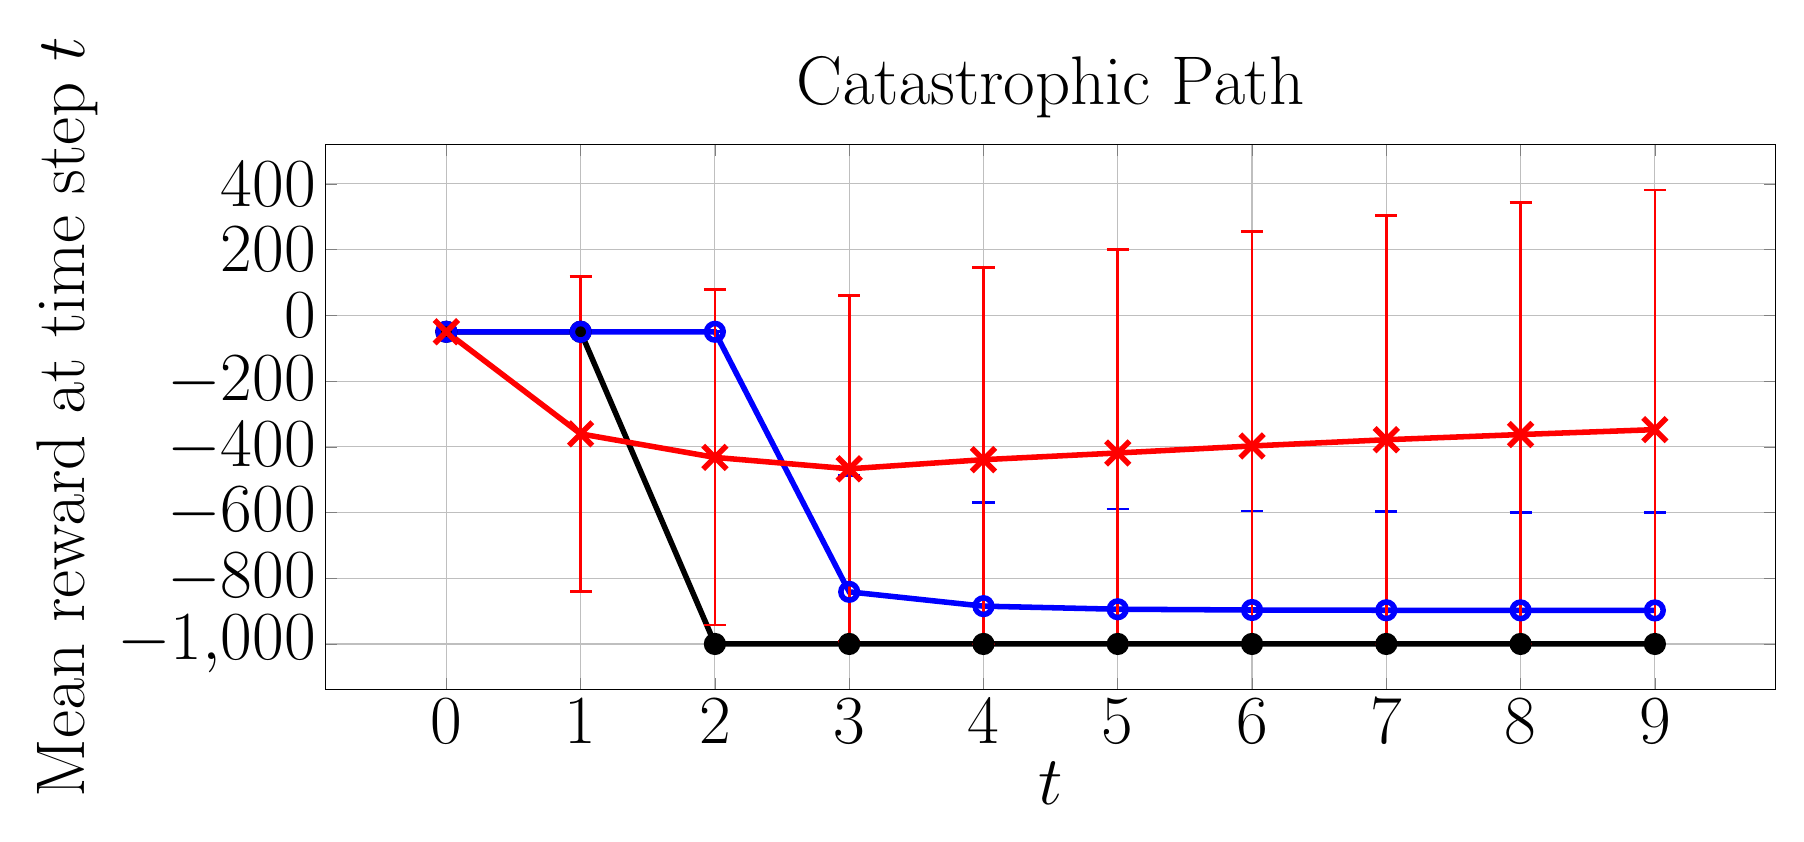
\begin{tikzpicture}
                \begin{axis}[
                    xlabel={$t$},
                    ylabel={Mean reward at time step $t$},
                    title={Catastrophic Path},
                    grid=both,
                    width=20cm, height=8.5cm,
                    every axis/.style={font=\Huge},
                    %
                ]
               \addplot[
                    color=black, %
                    mark=*, %
                    line width=2pt,
                    mark size=3pt,
                ]
                coordinates {
                    (0, -50.0)
                    (1, -50.0)
                    (2, -1000.0)
                    (3, -1000.0)
                    (4, -1000.0)
                    (5, -1000.0)
                    (6, -1000.0)
                    (7, -1000.0)
                    (8, -1000.0)
                    (9, -1000.0)
                };
                %
                %
                \addplot[
                    color=blue, %
                    mark=o, %
                    line width=2pt,
                    mark size=3pt,
                    error bars/.cd,
                    y dir=both, %
                    y explicit, %
                    error bar style={line width=1pt,solid},
                    error mark options={line width=1pt,mark size=4pt,rotate=90}
                ]
                coordinates {
                    (0, -50.0)  +- (0, 0.0)
                    (1, -50.0)  +- (0, 0.0) 
                    (2, -50.0)  +- (0, 0.0) 
                    (3, -841.440725)  += (0, 354.24605512) -= (0, 158.559275)
                    (4, -884.98225)  += (0, 315.37519669) -= (0, 115.01775)
                    (5, -894.330425) += (0, 304.88572805) -= (0, 105.669575)
                    (6, -896.696175) += (0, 301.19954514) -= (0, 103.303825)
                    (7, -897.4635) += (0, 299.61791279) -= (0, 102.5365)
                    (8, -897.77595) += (0, 298.80392585) -= (0, 102.22405)
                    (9, -897.942975) += (0, 298.32920557) -= (0, 102.057025)
                };
                %
                \addplot[
                    color=red, %
                    mark=x, %
                    line width=2pt,
                    mark size=6pt,
                    error bars/.cd,
                    y dir=both, %
                    y explicit, %
                    error bar style={line width=1pt,solid},
                    error mark options={line width=1pt,mark size=4pt,rotate=90}
                ]
            coordinates {
                    (0, -50.0)  +- (0, 0.0)
                    (1, -360.675265)  +- (0, 479.39812699) 
                    (2, -432.27629)  +- (0, 510.38620897) 
                    (3, -467.029545)  += (0, 526.36009628) -= (0, 526.36009628)
                    (4, -439.17429)  += (0, 583.96638919) -= (0, 560.82571)
                    (5, -418.82704) += (0, 618.43027478) -= (0, 581.17296)
                    (6, -397.464895) += (0, 652.67322574) -= (0, 602.535105)
                    (7, -378.49052) += (0, 682.85407033) -= (0, 621.50948)
                    (8, -362.654195) += (0, 707.01412023) -= (0, 637.345805)
                    (9, -347.737935) += (0, 729.29076479) -= (0, 652.262065)
                };
                %
                %
                %
                %
                %
                %
                %
                %
                %
                %
                %
                %
                %
                %
                %
                %
                %
                %
                %
                \end{axis}
            \end{tikzpicture}
         }
    }
    \caption{Average instant reward of CF paths induced by policies on Sepsis.}
    \label{fig: reward sepsis}
\end{figure*}

%
%
%
\subsection{Interval CFMDP Bounds}
%
%
Table \ref{tab:nonzero_probs} presents the mean counterfactual probability bound widths (excluding transitions where the upper bound is $0$) for each MDP, averaged over 20 observed paths. We compare the bounds under counterfactual stability (CS) and monotonicity (M) assumptions, CS alone, and no assumptions. This shows that the assumptions marginally reduce the bound widths, indicating the assumptions tighten the bounds without excluding too many causal models, as intended.
\renewcommand{\arraystretch}{1}

\begin{table}
\centering
\caption{Mean width of counterfactual probability bounds}
\resizebox{0.8\columnwidth}{!}{%
\begin{tabular}{|c|c|c|c|}
\hline
\multirow{2}{*}{\textbf{Environment}} & \multicolumn{3}{c|}{\textbf{Assumptions}} \\ \cline{2-4}
 & \textbf{CS + M} & \textbf{CS} & \textbf{None\tablefootnote{\jl{Equivalent to \citet{li2024probabilities}'s bounds (see Section \ref{sec: equivalence with Li}).}}} \\ \hline
\textbf{GridWorld} ($p=0.9$) & 0.0817 & 0.0977 & 0.100 \\ \hline
\textbf{GridWorld} ($p=0.4$) & 0.552  & 0.638  & 0.646 \\ \hline
\textbf{Sepsis} & 0.138 & 0.140 & 0.140 \\ \hline
\end{tabular}
}
\label{tab:nonzero_probs}
\end{table}


\subsection{Execution Times}
Table \ref{tab: times} compares the average time needed to generate the interval CFMDP vs.\ the Gumbel-max SCM CFMDP for 20 observations.
The GridWorld algorithms were run single-threaded, while the Sepsis experiments were run in parallel.
Generating the interval CFMDP is significantly faster as it uses exact analytical bounds, whereas the Gumbel-max CFMDP requires sampling from the Gumbel distribution to estimate counterfactual transition probabilities. \jl{Since constructing the counterfactual MDP models is the main bottleneck in both approaches, ours is more efficient overall and suitable for larger MDPs.}
\begin{table}
\centering
\caption{Mean execution time to generate CFMDPs}
\resizebox{0.99\columnwidth}{!}{%
\begin{tabular}{|c|c|c|}
\hline
\multirow{2}{*}{\textbf{Environment}} & \multicolumn{2}{c|}{\textbf{Mean Execution Time (s)}} \\ \cline{2-3} 
                                      & \textbf{Interval CFMDP} & \textbf{Gumbel-max CFMDP} \\ \hline
\textbf{GridWorld ($p=0.9$) }                  & 0.261                   & 56.1                      \\ \hline
\textbf{GridWorld ($p=0.4$)  }                 & 0.336                   & 54.5                      \\ \hline
\textbf{Sepsis}                                 & 688                     & 2940                      \\ \hline
\end{tabular}%
}
\label{tab: times}
\end{table}


\section{Discussion}
\RR{
Our study utilizes an intuitive flower-based visual design and evidence-based collaborative programming process analysis to provide instructors with a clear perspective for evaluating group and individual performance in collaborative programming. In this section, we discuss the lessons learned, the factors contributing to the research outcomes, and how these findings relate to existing works.

\subsection{Flower-Based Visual Design for Intuitive and Useful by Participants}
In large-scale learning analytics, intuitive visualization and interactive features prove to be valuable in assisting instructors with evaluations while reducing their workload~\cite{martinez2020data,fernandez2024data}.
Our study shows that the flower-based visual design effectively helps instructors summarize the performance of students and groups in collaborative programming.
Participants using \textit{CPVis} typically report starting by observing the flower visualization to gain an overview of the group's overall performance and the engagement levels of individual members during collaboration. Our design enables them to make quick assessment judgments and uncover valuable educational insights. 
For instance, students playing the Driver role often exhibit higher engagement levels.
\RA{Previous works use dynamic natural metaphors~\cite{tausch2014groupgarden,tausch2016comparison}, such as blooming flowers, falling leaves, and weather changes, to represent the quality and state of group discussions. However, these metaphors primarily convey overall trends or atmospheres rather than offering a precise and structured representation of multidimensional data, making it difficult for users to extract specific and accurate information efficiently. Moreover, the strong symbolic and emotional nature of their metaphors often leads to subjective interpretations.}
The effectiveness of our design lies in its ability to translate multiple dimensions of process-based learning analytics into visual elements such as colored petals and flower stamens, enabling instructors to quickly interpret multidimensional data and assess both group and individual performance during collaboration.
Furthermore, the flower-based visualization supports hierarchical analysis at both the group and individual levels, allowing instructors to efficiently analyze and compare the performance of multiple groups and students on a large scale.

\subsection{\textit{CPVis} Enhanced Instructors' Confidence in Evaluating Groups and Students}
The study demonstrates that \textit{CPVis} enhances participants' confidence in evaluation outcomes and improves the accuracy of their assessments. In Baseline System 1, participants report that accessing data requires significant time, and evaluating a specific group's performance often necessitates finding similar groups for a relatively fair comparison. 
Such a process demands additional time, causing participants to lose patience and avoid thoroughly examining all the details.
In baseline system 2, participants have to manually browse and process large amounts of student behavior and interaction data, which significantly increases cognitive load and reduces efficiency as they rely on memory to evaluate the performance of different groups.
In comparison, \textit{CPVis} offers significant convenience to participants \RA{by visualizing multidimensional learning analytics data}, allowing them to effortlessly access key information required for evaluations and compare similar groups. By providing both an overall view of multiple groups and detailed comparisons into individual groups, \textit{CPVis} substantially boosts participants' confidence in their evaluation outcomes, as demonstrated in the ratings. 
%This finding aligns with previous research results~\cite{sato2023groupnamics}.
\RA{Clear and intuitive visual analytics systems contribute to improved confidence and efficiency among participants. For instance, Groupnamics helps participants identify groups requiring intervention by visualizing each group's recent vocal activities and discussion statuses in a one-page view, thereby boosting their confidence in decision-making~\cite{sato2023groupnamics}.}
While it is ideal for \textit{CPVis} to support comparisons across an unlimited number of groups, practical limitations related to cognitive load and visual design make this challenging. Future efforts focus on optimizing the evaluation process through visual design, striking a balance between cognitive load and evaluation efficiency, thereby providing effective support for teaching.



\subsection{Theory-driven and LLM-powered Automation Evaluation for Quantifying Collaborative Learning}
Our study utilizes data collection, analysis, and visualization techniques to extract key insights from students' collaborative behaviors and outcomes, providing a deeper understanding of the learning process in collaborative programming. We focus on quantifying complex collaborative learning processes by leveraging LLMs and theoretical frameworks, introducing innovative methods to evaluate collaboration efficiency. 
While collaborative problem-solving is clearly defined in prior research~\cite{rosen2020towards}, achieving a quantitative balance between task performance and team effectiveness remains a significant challenge. To address this, we employ the coefficient of variation as a balancing metric and validate its efficacy using real-world datasets.
By integrating LLMs, \textit{CPVis} automates the annotation of collaborative programming performance, significantly reducing the workload associated with manually labeling large-scale classroom data and offering a novel perspective for automated learning analytics. 
Combining theory-driven metrics and LLM-powered automation provides instructors with robust, multidimensional evidence, enabling them to process and compare extensive student data systematically. 
This empowers instructors to effectively evaluate group and individual behaviors in collaborative programming, identify collaboration patterns, and support evidence-based decision-making. Previous research demonstrates that data-driven analysis helps educational decision-makers~\cite{hou2024codetailor}, such as instructors, uncover hidden learning patterns and deliver personalized guidance. Building on this foundation, \textit{CPVis} further enhances the potential for personalized feedback, enabling instructors to provide precise, data-driven guidance to students.


}


\section{Limitations and Future Work}

\RR{
In this section, we discuss the limitations of the current study and potential future work.
\subsection{Limitation}
Our study has three main limitations.
First, our current analysis is limited to data from a single real-world classroom's collaborative programming discussions, restricting the generalizability of our findings to other contexts. Similarly, our evaluation of \textit{CPVis} relies on a sampled dataset, limiting the study's scope. We hypothesize that participants working with smaller datasets and visualized learning analytics experience reduced cognitive load and find it easier to identify collaboration patterns due to fewer visual elements to process. However, in large-scale collaborative programming classrooms, instructors face the challenge of evaluating more groups and students, which may increase memory load and visual complexity.
Second, the data collected in our study are obtained from real classroom environments, maintaining ecological validity by capturing natural behaviors such as group silence or requests for instructor assistance. However, due to the limitations of non-intrusive equipment, our data lack details such as facial expressions and non-verbal cues. While participants report the comprehensiveness and richness of the learning analytics in the experiment, the absence of these data poses challenges for deeper analysis of emotional expressions and social engagement during collaborative programming. This limitation hinders the provision of a more holistic learning analysis for evaluation purposes.
Additionally, the recorded data are independent and exclude audio information, making it difficult to align screen interactions with dialogue streams. This limitation constrains the exploration of the relationship between collaborative behavior patterns and collaborative problem-solving processes.
Finally, in large-scale collaborative programming classrooms, generating analytics using LLMs requires significant computational time and cost. While feasible for institutions with robust computational resources, this remains a limitation for deploying such tools in real teaching scenarios. Furthermore, in real classrooms, noise from multiple group discussions introduces significant data noise, complicating the automation of learning analytics generation and limiting the accuracy of evaluations for groups and individual students.


\subsection{Future Work}
Without well-structured visualizations, simply presenting multiple data streams poses significant challenges for instructors attempting to interpret these large-scale datasets~\cite{fernandez2024data}.
In this study, we explore the integration and analysis of multimodal data. However, \textit{CPVis} has the potential to further enhance the visualization and perception of multimodal data, enabling instructors to evaluate group and student performance with greater accuracy and reduced cognitive load~\cite{martinez2020data}. 
Our target audience consists of instructors teaching large introductory collaborative programming courses, who require more efficient and intuitive visualizations to understand student performance during collaboration.  
While our use of static 2D visualizations, such as high-dimensional flower glyphs, has been highly regarded by participants for boosting confidence and helping instructors quickly identify key features, we believe there is room for improvement in organizing visualization formats to enhance information transmission efficiency and the users cognitive experience.
For instance, incorporating narrative visualizations further streamlines the process by allowing instructors to generate composite evaluations based on their weighting of different collaboration performance dimensions~\cite{gratzl2013lineup}. 
Narrative visualizations enable instructors to delve into data details, organize learning analytics results along logical paths such as timelines, causality, or categories, and highlight key information~\cite{chen2019designing}. 
This approach mitigates visual overload caused by excessive data, significantly reduces the time and cognitive effort required for evaluation, and ultimately supports instructors in making better decisions and assessments.

\textit{CPVis} requires instructors to spend additional time after class to evaluate collaborative performance. In our study, most participants indicate during follow-up interviews that the extra time spent on evaluating students' collaborative performance is highly valuable for producing comprehensive assessments. They note that providing immediate evaluations during the collaboration process is unrealistic, as final assessments typically need a holistic consideration of task completion and group dynamics after class. However, there is a significant demand for real-time analysis tools to deliver timely, personalized feedback to students and offer appropriate instructional scaffolding during the collaborative process~\cite{tang2024sphere}.
Instructors frequently find themselves overwhelmed by the immediate needs of some students~\cite{yang2023pair}, unintentionally neglecting others. To address this issue, future work could explore the integration of LLMs to enable real-time monitoring and analysis of students' behavioral data—such as code submissions, error logs, and engagement levels. LLMs could automatically detect learning bottlenecks or collaboration issues, providing instant feedback on common problems to students. This would effectively reduce instructors' workload, allowing them to focus on complex or critical issues, and simplify classroom management tasks.
For instance, LLMs could summarize patterns in students' code submissions and generate a ``hotspot report'' identifying recurring issues across the class. They could also provide real-time collaborative performance analytics for different groups, enabling instructors to quickly gain a comprehensive understanding of overall class dynamics. Additionally, LLMs could assist in role allocation within groups, suggest strategies to improve team interactions, and identify potential conflicts or disengagement within collaborative teams.
LLM-powered tools automate evaluations and enable personalized feedback, bridging post-class assessments with in-class scaffolding to enhance teaching and learning in collaborative programming.}
\section{Conclusion}
In this work, we propose a simple yet effective approach, called SMILE, for graph few-shot learning with fewer tasks. Specifically, we introduce a novel dual-level mixup strategy, including within-task and across-task mixup, for enriching the diversity of nodes within each task and the diversity of tasks. Also, we incorporate the degree-based prior information to learn expressive node embeddings. Theoretically, we prove that SMILE effectively enhances the model's generalization performance. Empirically, we conduct extensive experiments on multiple benchmarks and the results suggest that SMILE significantly outperforms other baselines, including both in-domain and cross-domain few-shot settings.

%%
%% The acknowledgments section is defined using the "acks" environment
%% (and NOT an unnumbered section). This ensures the proper
%% identification of the section in the article metadata, and the
%% consistent spelling of the heading.
\begin{acks}
Meng Xia is the corresponding author.
The work was supported by the National Natural Science Foundation of China, (62422607, 62372411, 62036009) and the Zhejiang Provincial Natural Science Foundation of China.

\end{acks}
%%
%% This is file `sample-sigconf-authordraft.tex',
%% generated with the docstrip utility.
%%
%% The original source files were:
%%
%% samples.dtx  (with options: `all,proceedings,bibtex,authordraft')
%% 
%% IMPORTANT NOTICE:
%% 
%% For the copyright see the source file.
%% 
%% Any modified versions of this file must be renamed
%% with new filenames distinct from sample-sigconf-authordraft.tex.
%% 
%% For distribution of the original source see the terms
%% for copying and modification in the file samples.dtx.
%% 
%% This generated file may be distributed as long as the
%% original source files, as listed above, are part of the
%% same distribution. (The sources need not necessarily be
%% in the same archive or directory.)
%%
%%
%% Commands for TeXCount
%TC:macro \cite [option:text,text]
%TC:macro \citep [option:text,text]
%TC:macro \citet [option:text,text]
%TC:envir table 0 1
%TC:envir table* 0 1
%TC:envir tabular [ignore] word
%TC:envir displaymath 0 word
%TC:envir math 0 word
%TC:envir comment 0 0
%%
%%
%% The first command in your LaTeX source must be the \documentclass
%% command.
%%
%% For submission and review of your manuscript please change the
%% command to \documentclass[manuscript, screen, review]{acmart}.
%%
%% When submitting camera ready or to TAPS, please change the command
%% to \documentclass[sigconf]{acmart} or whichever template is required
%% for your publication.
%%
%%
\documentclass[sigconf, nonacm]{acmart}
%\documentclass[sigconf]{acmart}
%\documentclass[sigconf,authordraft]{acmart}
%\documentclass[anonymous,manuscript,review]{acmart}

%%
%% \BibTeX command to typeset BibTeX logo in the docs
\AtBeginDocument{%
  \providecommand\BibTeX{{%
    Bib\TeX}}}

%% Rights management information.  This information is sent to you
%% when you complete the rights form.  These commands have SAMPLE
%% values in them; it is your responsibility as an author to replace
%% the commands and values with those provided to you when you
%% complete the rights form.
%\setcopyright{acmlicensed}
\copyrightyear{2025}
\acmYear{2025}
%\setcopyright{cc}
\setcctype{by}
\acmConference[CHI '25]{CHI Conference on Human Factors in Computing Systems}{April 26-May 1, 2025}{Yokohama, Japan}
\acmBooktitle{CHI Conference on Human Factors in Computing Systems (CHI '25), April 26-May 1, 2025, Yokohama, Japan}
\acmDOI{10.1145/3706598.3713353}
\acmISBN{979-8-4007-1394-1/25/04}


%%
%% Submission ID.
%% Use this when submitting an article to a sponsored event. You'll
%% receive a unique submission ID from the organizers
%% of the event, and this ID should be used as the parameter to this command.
%%\acmSubmissionID{123-A56-BU3}

%%
%% For managing citations, it is recommended to use bibliography
%% files in BibTeX format.
%%
%% You can then either use BibTeX with the ACM-Reference-Format style,
%% or BibLaTeX with the acmnumeric or acmauthoryear sytles, that include
%% support for advanced citation of software artefact from the
%% biblatex-software package, also separately available on CTAN.
%%
%% Look at the sample-*-biblatex.tex files for templates showcasing
%% the biblatex styles.
%%

%%
%% The majority of ACM publications use numbered citations and
%% references.  The command \citestyle{authoryear} switches to the
%% "author year" style.
%%
%% If you are preparing content for an event
%% sponsored by ACM SIGGRAPH, you must use the "author year" style of
%% citations and references.
%% Uncommenting
%% the next command will enable that style.
%%\citestyle{acmauthoryear}
\usepackage{booktabs}
\usepackage{graphicx}
\usepackage{listings}
\usepackage{xcolor} 
\usepackage{caption}
%\usepackage{paralist}
\usepackage{makecell}
\usepackage{url}
\usepackage{longtable}
\usepackage{color}
\usepackage{tikz}
%\usepackage[utf8]{enc}
\usepackage[T1]{fontenc}
\usepackage{lipsum}
\usepackage{stfloats}
\usepackage{tabu} 
\usepackage{tabularx}
\usepackage{multirow}
\usepackage{booktabs}
\usepackage{graphicx}
\usepackage{wrapfig}
\usepackage{hyperref}   
\usepackage{cleveref}
%\usepackage[most]{tcolorbox} 
\usepackage{xcolor}
\usepackage{float}
\usepackage{listings} 
%\usepackage{tcolorbox}




\definecolor{PurpleColor}{RGB}{0,0,0}
\newcommand{\RR}[1]{{\color{PurpleColor}#1}}

\definecolor{PinkColor}{RGB}{0, 0, 0}
\newcommand{\RA}[1]{{\color{PinkColor}#1}}


\definecolor{codegreen}{rgb}{0,0.6,0}
\definecolor{codegray}{rgb}{0.5,0.5,0.5}
\definecolor{codepurple}{rgb}{0.58,0,0.82}
\definecolor{backcolour}{rgb}{0.95,0.95,0.92}

\lstdefinestyle{mystyle}{
  backgroundcolor=\color{backcolour}, commentstyle=\color{codegreen},
  keywordstyle=\color{magenta},
  numberstyle=\tiny\color{codegray},
  stringstyle=\color{codepurple},
  basicstyle=\ttfamily\footnotesize,
  breakatwhitespace=false,         
  breaklines=true,                 
  captionpos=b,                    
  keepspaces=true,                 
  numbers=left,                    
  numbersep=5pt,                  
  showspaces=false,                
  showstringspaces=false,
  showtabs=false,                  
  tabsize=2
}
\lstset{style=mystyle}


%\definecolor{PurpleColor}{RGB}{0,0,0}

%%
%% end of the preamble, start of the body of the document source.
\begin{document}

%%
%% The "title" command has an optional parameter,
%% allowing the author to define a "short title" to be used in page headers.
\title{CPVis: Evidence-based Multimodal Learning Analytics for Evaluation in Collaborative Programming}

%%
%% The "author" command and its associated commands are used to define
%% the authors and their affiliations.
%% Of note is the shared affiliation of the first two authors, and the
%% "authornote" and "authornotemark" commands
%% used to denote shared contribution to the research.
\author{Gefei Zhang}
\affiliation{%
  \institution{Zhejiang University of Technology}
  \city{Hangzhou}
  \state{Zhejiang}
  \country{China}}
\email{gefei@zjut.edu.cn}
\orcid{1234-5678-9012}

\author{Shenming Ji}
\affiliation{%
  \institution{Xi'an Jiaotong-Liverpool University}
  \city{Suzhou}
  \state{Jiangsu}
  \country{China}}
\email{shenming.ji21@student.xjtlu.edu.cn}

\author{Yicao Li}
\affiliation{%
  \institution{Zhejiang University of Technology}
  \city{Hangzhou}
  \state{Zhejiang}
  \country{China}}
\email{yicaoli47@gmail.com}

\author{Jingwei Tang}
\affiliation{%
  \institution{Zhejiang University of Technology}
  \city{Hangzhou}
  \state{Zhejiang}
  \country{China}}
\email{jwtang@zjut.edu.cn}

\author{Jihong Ding}
\affiliation{%
 \institution{Hannan University}
 \city{Haikou}
 \state{Hainan}
 \country{China}}
\email{jhding@hainanu.edu.cn}

\author{Meng Xia}
\affiliation{%
  \institution{Texas A\&M University}
  \city{College Station}
  \state{Texas}
  \country{USA}}
\email{mengxia@tamu.edu}

\author{Guodao Sun}
\affiliation{%
  \institution{Zhejiang University of Technology}
  \city{Hangzhou}
  \state{Zhejiang}
  \country{China}}
\email{guodao@zjut.edu.cn}

\author{Ronghua Liang}
\affiliation{%
  \institution{Zhejiang University of Technology}
  \city{Hangzhou}
  \state{Zhejiang}
  \country{China}}
\email{rhliang@zjut.edu.cn}



%%
%% By default, the full list of authors will be used in the page
%% headers. Often, this list is too long, and will overlap
%% other information printed in the page headers. This command allows
%% the author to define a more concise list
%% of authors' names for this purpose.
\renewcommand{\shortauthors}{Zhang et al.}

%%
%% The abstract is a short summary of the work to be presented in the
%% article.
\begin{abstract}
As programming education becomes more widespread, many college students from non-computer science backgrounds begin learning programming. Collaborative programming emerges as an effective method for instructors to support novice students in developing coding and teamwork abilities. However, due to limited class time and attention, instructors face challenges in monitoring and evaluating the progress and performance of groups or individuals. To address this issue, we collect multimodal data from real-world settings and develop \textit{CPVis}, \RR{an interactive visual analytics system designed to assess student collaboration dynamically.} Specifically, \textit{CPVis} enables instructors to evaluate both group and individual performance efficiently. \textit{CPVis} employs a novel flower-based visual encoding to represent performance and provides time-based views to capture the evolution of collaborative behaviors. A within-subject experiment (N=22), \RR{comparing \textit{CPVis} with two baseline systems, reveals that users gain more insights, find the visualization more intuitive, and report increased confidence in their assessments of collaboration.}
\end{abstract}

%%
%% The code below is generated by the tool at http://dl.acm.org/ccs.cfm.
%% Please copy and paste the code instead of the example below.
%%

\begin{CCSXML}
<ccs2012>
   <concept>
       <concept_id>10010405.10010489.10010492</concept_id>
       <concept_desc>Applied computing~Collaborative learning</concept_desc>
       <concept_significance>500</concept_significance>
       </concept>
 </ccs2012>
\end{CCSXML}

\begin{CCSXML}
<ccs2012>
   <concept>
       <concept_id>10003120.10003145.10003151</concept_id>
       <concept_desc>Human-centered computing~Visualization systems and tools</concept_desc>
       <concept_significance>500</concept_significance>
       </concept>
 </ccs2012>
\end{CCSXML}

\ccsdesc[500]{Human-centered computing~Visualization systems and tools}

\ccsdesc[500]{Applied computing~Collaborative learning}


\begin{comment}



\end{comment}
%%
%% Keywords. The author(s) should pick words that accurately describe
%% the work being presented. Separate the keywords with commas.
\keywords{Group visualization, education visualization, collaborative programming}
%% A "teaser" image appears between the author and affiliation
%% information and the body of the document, and typically spans the
%% page.








% \received{20 February 2007}
% \received[revised]{12 March 2009}
% \received[accepted]{5 June 2009}

%%
%% This command processes the author and affiliation and title
%% information and builds the first part of the formatted document.
\maketitle
%\newtcbox{\inlinecode}{on line, colback=gray!10, colframe=gray!10, boxrule=0.1mm, 
%	rounded corners, fontupper=\bfseries, left=0.1mm, right=0.1mm, top=0.1mm, bottom=0.1mm}

\section{Introduction}
\label{sec:introduction}
The business processes of organizations are experiencing ever-increasing complexity due to the large amount of data, high number of users, and high-tech devices involved \cite{martin2021pmopportunitieschallenges, beerepoot2023biggestbpmproblems}. This complexity may cause business processes to deviate from normal control flow due to unforeseen and disruptive anomalies \cite{adams2023proceddsriftdetection}. These control-flow anomalies manifest as unknown, skipped, and wrongly-ordered activities in the traces of event logs monitored from the execution of business processes \cite{ko2023adsystematicreview}. For the sake of clarity, let us consider an illustrative example of such anomalies. Figure \ref{FP_ANOMALIES} shows a so-called event log footprint, which captures the control flow relations of four activities of a hypothetical event log. In particular, this footprint captures the control-flow relations between activities \texttt{a}, \texttt{b}, \texttt{c} and \texttt{d}. These are the causal ($\rightarrow$) relation, concurrent ($\parallel$) relation, and other ($\#$) relations such as exclusivity or non-local dependency \cite{aalst2022pmhandbook}. In addition, on the right are six traces, of which five exhibit skipped, wrongly-ordered and unknown control-flow anomalies. For example, $\langle$\texttt{a b d}$\rangle$ has a skipped activity, which is \texttt{c}. Because of this skipped activity, the control-flow relation \texttt{b}$\,\#\,$\texttt{d} is violated, since \texttt{d} directly follows \texttt{b} in the anomalous trace.
\begin{figure}[!t]
\centering
\includegraphics[width=0.9\columnwidth]{images/FP_ANOMALIES.png}
\caption{An example event log footprint with six traces, of which five exhibit control-flow anomalies.}
\label{FP_ANOMALIES}
\end{figure}

\subsection{Control-flow anomaly detection}
Control-flow anomaly detection techniques aim to characterize the normal control flow from event logs and verify whether these deviations occur in new event logs \cite{ko2023adsystematicreview}. To develop control-flow anomaly detection techniques, \revision{process mining} has seen widespread adoption owing to process discovery and \revision{conformance checking}. On the one hand, process discovery is a set of algorithms that encode control-flow relations as a set of model elements and constraints according to a given modeling formalism \cite{aalst2022pmhandbook}; hereafter, we refer to the Petri net, a widespread modeling formalism. On the other hand, \revision{conformance checking} is an explainable set of algorithms that allows linking any deviations with the reference Petri net and providing the fitness measure, namely a measure of how much the Petri net fits the new event log \cite{aalst2022pmhandbook}. Many control-flow anomaly detection techniques based on \revision{conformance checking} (hereafter, \revision{conformance checking}-based techniques) use the fitness measure to determine whether an event log is anomalous \cite{bezerra2009pmad, bezerra2013adlogspais, myers2018icsadpm, pecchia2020applicationfailuresanalysispm}. 

The scientific literature also includes many \revision{conformance checking}-independent techniques for control-flow anomaly detection that combine specific types of trace encodings with machine/deep learning \cite{ko2023adsystematicreview, tavares2023pmtraceencoding}. Whereas these techniques are very effective, their explainability is challenging due to both the type of trace encoding employed and the machine/deep learning model used \cite{rawal2022trustworthyaiadvances,li2023explainablead}. Hence, in the following, we focus on the shortcomings of \revision{conformance checking}-based techniques to investigate whether it is possible to support the development of competitive control-flow anomaly detection techniques while maintaining the explainable nature of \revision{conformance checking}.
\begin{figure}[!t]
\centering
\includegraphics[width=\columnwidth]{images/HIGH_LEVEL_VIEW.png}
\caption{A high-level view of the proposed framework for combining \revision{process mining}-based feature extraction with dimensionality reduction for control-flow anomaly detection.}
\label{HIGH_LEVEL_VIEW}
\end{figure}

\subsection{Shortcomings of \revision{conformance checking}-based techniques}
Unfortunately, the detection effectiveness of \revision{conformance checking}-based techniques is affected by noisy data and low-quality Petri nets, which may be due to human errors in the modeling process or representational bias of process discovery algorithms \cite{bezerra2013adlogspais, pecchia2020applicationfailuresanalysispm, aalst2016pm}. Specifically, on the one hand, noisy data may introduce infrequent and deceptive control-flow relations that may result in inconsistent fitness measures, whereas, on the other hand, checking event logs against a low-quality Petri net could lead to an unreliable distribution of fitness measures. Nonetheless, such Petri nets can still be used as references to obtain insightful information for \revision{process mining}-based feature extraction, supporting the development of competitive and explainable \revision{conformance checking}-based techniques for control-flow anomaly detection despite the problems above. For example, a few works outline that token-based \revision{conformance checking} can be used for \revision{process mining}-based feature extraction to build tabular data and develop effective \revision{conformance checking}-based techniques for control-flow anomaly detection \cite{singh2022lapmsh, debenedictis2023dtadiiot}. However, to the best of our knowledge, the scientific literature lacks a structured proposal for \revision{process mining}-based feature extraction using the state-of-the-art \revision{conformance checking} variant, namely alignment-based \revision{conformance checking}.

\subsection{Contributions}
We propose a novel \revision{process mining}-based feature extraction approach with alignment-based \revision{conformance checking}. This variant aligns the deviating control flow with a reference Petri net; the resulting alignment can be inspected to extract additional statistics such as the number of times a given activity caused mismatches \cite{aalst2022pmhandbook}. We integrate this approach into a flexible and explainable framework for developing techniques for control-flow anomaly detection. The framework combines \revision{process mining}-based feature extraction and dimensionality reduction to handle high-dimensional feature sets, achieve detection effectiveness, and support explainability. Notably, in addition to our proposed \revision{process mining}-based feature extraction approach, the framework allows employing other approaches, enabling a fair comparison of multiple \revision{conformance checking}-based and \revision{conformance checking}-independent techniques for control-flow anomaly detection. Figure \ref{HIGH_LEVEL_VIEW} shows a high-level view of the framework. Business processes are monitored, and event logs obtained from the database of information systems. Subsequently, \revision{process mining}-based feature extraction is applied to these event logs and tabular data input to dimensionality reduction to identify control-flow anomalies. We apply several \revision{conformance checking}-based and \revision{conformance checking}-independent framework techniques to publicly available datasets, simulated data of a case study from railways, and real-world data of a case study from healthcare. We show that the framework techniques implementing our approach outperform the baseline \revision{conformance checking}-based techniques while maintaining the explainable nature of \revision{conformance checking}.

In summary, the contributions of this paper are as follows.
\begin{itemize}
    \item{
        A novel \revision{process mining}-based feature extraction approach to support the development of competitive and explainable \revision{conformance checking}-based techniques for control-flow anomaly detection.
    }
    \item{
        A flexible and explainable framework for developing techniques for control-flow anomaly detection using \revision{process mining}-based feature extraction and dimensionality reduction.
    }
    \item{
        Application to synthetic and real-world datasets of several \revision{conformance checking}-based and \revision{conformance checking}-independent framework techniques, evaluating their detection effectiveness and explainability.
    }
\end{itemize}

The rest of the paper is organized as follows.
\begin{itemize}
    \item Section \ref{sec:related_work} reviews the existing techniques for control-flow anomaly detection, categorizing them into \revision{conformance checking}-based and \revision{conformance checking}-independent techniques.
    \item Section \ref{sec:abccfe} provides the preliminaries of \revision{process mining} to establish the notation used throughout the paper, and delves into the details of the proposed \revision{process mining}-based feature extraction approach with alignment-based \revision{conformance checking}.
    \item Section \ref{sec:framework} describes the framework for developing \revision{conformance checking}-based and \revision{conformance checking}-independent techniques for control-flow anomaly detection that combine \revision{process mining}-based feature extraction and dimensionality reduction.
    \item Section \ref{sec:evaluation} presents the experiments conducted with multiple framework and baseline techniques using data from publicly available datasets and case studies.
    \item Section \ref{sec:conclusions} draws the conclusions and presents future work.
\end{itemize}
\putsec{related}{Related Work}

\noindent \textbf{Efficient Radiance Field Rendering.}
%
The introduction of Neural Radiance Fields (NeRF)~\cite{mil:sri20} has
generated significant interest in efficient 3D scene representation and
rendering for radiance fields.
%
Over the past years, there has been a large amount of research aimed at
accelerating NeRFs through algorithmic or software
optimizations~\cite{mul:eva22,fri:yu22,che:fun23,sun:sun22}, and the
development of hardware
accelerators~\cite{lee:cho23,li:li23,son:wen23,mub:kan23,fen:liu24}.
%
The state-of-the-art method, 3D Gaussian splatting~\cite{ker:kop23}, has
further fueled interest in accelerating radiance field
rendering~\cite{rad:ste24,lee:lee24,nie:stu24,lee:rho24,ham:mel24} as it
employs rasterization primitives that can be rendered much faster than NeRFs.
%
However, previous research focused on software graphics rendering on
programmable cores or building dedicated hardware accelerators. In contrast,
\name{} investigates the potential of efficient radiance field rendering while
utilizing fixed-function units in graphics hardware.
%
To our knowledge, this is the first work that assesses the performance
implications of rendering Gaussian-based radiance fields on the hardware
graphics pipeline with software and hardware optimizations.

%%%%%%%%%%%%%%%%%%%%%%%%%%%%%%%%%%%%%%%%%%%%%%%%%%%%%%%%%%%%%%%%%%%%%%%%%%
\myparagraph{Enhancing Graphics Rendering Hardware.}
%
The performance advantage of executing graphics rendering on either
programmable shader cores or fixed-function units varies depending on the
rendering methods and hardware designs.
%
Previous studies have explored the performance implication of graphics hardware
design by developing simulation infrastructures for graphics
workloads~\cite{bar:gon06,gub:aam19,tin:sax23,arn:par13}.
%
Additionally, several studies have aimed to improve the performance of
special-purpose hardware such as ray tracing units in graphics
hardware~\cite{cho:now23,liu:cha21} and proposed hardware accelerators for
graphics applications~\cite{lu:hua17,ram:gri09}.
%
In contrast to these works, which primarily evaluate traditional graphics
workloads, our work focuses on improving the performance of volume rendering
workloads, such as Gaussian splatting, which require blending a huge number of
fragments per pixel.

%%%%%%%%%%%%%%%%%%%%%%%%%%%%%%%%%%%%%%%%%%%%%%%%%%%%%%%%%%%%%%%%%%%%%%%%%%
%
In the context of multi-sample anti-aliasing, prior work proposed reducing the
amount of redundant shading by merging fragments from adjacent triangles in a
mesh at the quad granularity~\cite{fat:bou10}.
%
While both our work and quad-fragment merging (QFM)~\cite{fat:bou10} aim to
reduce operations by merging quads, our proposed technique differs from QFM in
many aspects.
%
Our method aims to blend \emph{overlapping primitives} along the depth
direction and applies to quads from any primitive. In contrast, QFM merges quad
fragments from small (e.g., pixel-sized) triangles that \emph{share} an edge
(i.e., \emph{connected}, \emph{non-overlapping} triangles).
%
As such, QFM is not applicable to the scenes consisting of a number of
unconnected transparent triangles, such as those in 3D Gaussian splatting.
%
In addition, our method computes the \emph{exact} color for each pixel by
offloading blending operations from ROPs to shader units, whereas QFM
\emph{approximates} pixel colors by using the color from one triangle when
multiple triangles are merged into a single quad.


\section{Formative Study} 
\label{sec:formative}
We conducted a formative study to explore instructors' challenges in collaborative programming and their visualization needs, with the study protocol approved by our university's Institutional Review Board (IRB).
 
 \subsection{Participants}
We recruited ten participants (five females, age: \(30.6 \pm 6.6\)) with collaborative programming experience, divided into three groups: two educational technology experts (E1, E2) and eight instructors (T1–T8) with an average of 8.14 years of teaching programming. Participants, recruited via snowball sampling from the authors' network, received \$20 as compensation.
 

\subsection{Procedure}\
\RR{The formative study used semi-structured interviews conducted via Zoom, divided into two sections: (A) Questions and Answers and (B) Ratings.}
\textit{A: Questions and Answers.} 
Each participant was independently interviewed to explore the need for collaborative programming analysis. Topics included teaching experience with collaborative programming, class organization, challenges faced, assessment methods, and group and individual performance evaluations. Follow-up questions were asked for clarification or more profound insights. Each session lasted 40–60 minutes and was documented through written notes, audio, and video recordings.
\textit{B: Rating.} 
Participants then rated two aspects of the collaborative programming visual analytics system. They rated feature importance (Q1) on a 1–7 scale (7 being the highest) and ranked features by priority (Q2). 
\RR{More details are in appendix A.}

 
\subsection{Findings} 

\begin{figure*}[htbp]
	\centering
	\includegraphics[width=1\linewidth]{scheme1.pdf}
	\caption{Collaborative programming coding schemes, along with their definitions and examples.}
        \Description{Collaborative programming coding schemes, along with their definitions and examples.}
	\label{fig:scheme}
\end{figure*}



\subsubsection{Evaluation of Groups:}
In large classes, instructors struggled to monitor each group without the help of teaching assistants. They often relied on group presentations (E2, T1, T5), but it was inaccurate. Limited class time forced instructors to focus on solving issues rather than actively monitoring groups.


\textbf{Group Performance:}
Evaluating group work was based on the final code rather than the process, limiting the ability to provide feedback (T7). Some instructors used presentations or technical documentation to streamline assessments (T6). However, evaluating more than 20 groups was still challenging, and instructor assistance was often overlooked during evaluations.


\textbf{Collaboration Evaluation:}
Effective collaboration wasn't just about task completion speed and group dynamics. Some groups (T7) completed tasks quickly due to one member's efforts, not true collaboration. 
\RR{E1 proposed the collaborative problem-solving framework to distinguish task effectiveness from team effectiveness.} Instructors (T6) believed monitoring discussion time helped assess collaboration quality and task difficulty, but off-topic discussions made it hard to evaluate group discussions (E1, T3, T5).


\subsubsection{Evaluation of Students:}

In large classes, assessing individual contributions in group work was challenging. Instructors relied on peer evaluations (T2, T3, T4) and self-reported task distributions (E2), which were often subjective.

\textbf{Individual Performance:}
Instructors typically reviewed code to assess understanding, but measuring individual contributions in group work was hard. Leadership roles often reflected a deeper grasp of concepts (T1), but tracking individual engagement was difficult in large classes.


\textbf{Personalized Feedback:}
Providing personalized feedback was difficult, as group results often masked individual struggles. T3 and T4 noted that group collaboration fostered peer learning but could lead to less engagement from weaker students.
\textit{T8 added that offering personalized feedback in large classes was time-consuming and burdensome.}

 
 
 
\subsection{Design requirement}
\label{dr}
Based on the interview findings, we identified six design requirements (R1–R6) across three levels, summarized as follows:

Support \textbf{\textit{inter-group-level}} to provide a macro perspective, enabling instructors to observe the overall situation of all groups comprehensively and fully understand class-wide dynamics.

\textbf{R1: Displaying the Overall Performance of all Groups.} 
Instructors face challenges in supervising multiple groups simultaneously and shifting focus efficiently. Participants stressed the need for an overview of group performance, allowing instructors to grasp class dynamics and selectively review specific groups.


\RR{\textbf{R2: Comparing Similar and Different Groups.} 
Instructors often compare students' performance to assess their relative standing within the class~\cite{marsh1997making}. Such comparisons enable a more accurate evaluation of group performance and help identify groups excelling or encountering challenges.}


Supporting \textbf{\textit{intra-group-level}} visual exploration to offer a meso perspective, enabling instructors to observe specific groups' performance and gain a comprehensive understanding of group dynamics during the collaborative programming process.


\textbf{ R3: Understand the Dynamics of Programming Problem Solving.}
Analyzing a group's evolving communication patterns and computational thinking during programming tasks provides instructors with deeper insights into students' progress and intermediate learning objectives—details missed in final submissions alone.


\textbf{ R4: Identify Teacher Scaffolding in Collaboration.}
Instructors play a vital role in guiding groups during collaborative programming. Understanding the scaffolding provided and students' responses can help refine instructional strategies, improving the overall effectiveness of collaborative programming.


Supporting \textbf{\textit{individual-student-level}} visual exploration to provide a micro perspective allows instructors to observe each student's performance within a specific group and better understand their role and collaboration.

\textbf{R5: Track Changes in Student Engagement Over Time.} 
Limited classroom time makes it challenging for instructors to monitor individual student engagement in programming tasks.
Tracking and visualizing engagement trends is essential for assessing performance and refining instructional practices.

\textbf{R6: Access Detailed Raw Data.} 
Instructors require access to raw data, such as collaboration videos, conversations, and background information. These details are crucial for validating analysis results and supporting personalized feedback and assessments.


% TODO
% more detailed introduction of dataset creation
% the rumour label in such datasets
\section{Data} \label{sec:data}
We use three rumour datasets in this work, namely: PHEME~\citep{pheme2015,kochkina-etal-2018-one}, Twitter15, and Twitter16~\citep{ma-etal-2017-detect}:

% TJB: how can the number of threads be greater than the number of tweets? these numbers don't make sense
% RX: fixed, the numbers were incorrect
\paragraph{PHEME}~\citet{pheme2015} contains 6,425 tweet posts of rumours and non-rumours related to 9 events. To avoid using specific a priori keywords to search for tweet posts, PHEME used the Twitter (now X) steaming API to identify newsworthy events from breaking news and then selected from candidate rumours that met rumour criteria, finally they collected associated conversations and annotate them. They engaged journalists to annotate the threads. The data were collected between 2014 and 2015. The 9 events are split into two groups, the first being breaking news that contains rumours, including Ferguson unrest, Ottawa shooting, Sydney siege, Charlie Hebdo shooting, and Germanwings plane crash. The rest are specific rumours, namely Prince to play in Toronto, Gurlitt collection, Putin missing, and Michael Essien contracting Ebola.
% TJB: say something about the time period when this data was collected
% RX: added

\paragraph{Twitter 15}~\citet{twitter15} was constructed by collecting rumour and non-rumour posts from the tracking websites snopes.com and emergent.info. They then used the Twitter API to gather corresponding posts, resulting in 94 true and 446 false posts. This dataset further includes 1,490 root posts and their follow posts, comprising 1,116 rumours and 374 non-rumours.
% TJB: the "tweet" vs. "comment" terminology is potentially confusing and needs to be clarified
% RX: unified, used root and follow posts to refer to root posts and the comment posts, posts are used to describe tweets in general.

\paragraph{Twitter 16}
Similarly to Twitter 15, \citet{twitter16} collected rumours and non-rumours from snopes.com, resulting in 778 reported events, 64\% of which are rumours. For each event, keywords were extracted from the final part of the Snopes URL and refined manually---adding, deleting, or replacing words iteratively---until the composed queries yielded precise Twitter search results. The final dataset includes 1,490 root tweet posts and their follow posts, comprising 613 rumours and 205 non-rumours.

\begin{table*}[!t]
    \centering
    \small
    \begin{tabular}{p{0.05\linewidth}p{0.9\linewidth}}
    \toprule
    Task & Prompt \\
    \midrule
    V-oc & Categorize the text into an ordinal class that best characterizes the writer's mental state, considering various degrees of positive and negative sentiment intensity. 3: very positive mental state can be inferred. 2: moderately positive mental state can be inferred. 1: slightly positive mental state can be inferred. 0: neutral or mixed mental state can be inferred. -1: slightly negative mental state can be inferred. -2: moderately negative mental state can be inferred. -3: very negative mental state can be inferred.\\
    \midrule
    E-c & Categorize the text's emotional tone as either `neutral or no emotion' or identify the presence of one or more of the given emotions (anger, anticipation, disgust, fear, joy, love, optimism, pessimism, sadness, surprise, trust).\\
    \midrule
    E-i & Assign a numerical value between 0 (least E) and 1 (most E) to represent the intensity of emotion E expressed in the text.\\
    \bottomrule
    \end{tabular}
    \caption{Prompts used for EmoLLM to detect emotion information in tweets. V-oc = Valence Ordinal Classification, E-c = Emotion Classification, and E-i = Emotion Intensity Regression.}
    \label{tab:emollm_ins}
\end{table*}


  
%%% Local Variables:
%%% mode: latex
%%% TeX-master: "../main_anonymous"
%%% End:




\section{System Design} 
\label{sec:vis}

In this session, we introduce \textit{CPVis} (Fig.~\ref{fig:teaser}), a web-based visual analytics system to assist instructors in evaluating collaborative programming.
\subsection{System Overview}
\textit{CPVis} is a comprehensive system supporting multi-level, progressive analysis, from group-level interactions to individual student performance. Instructors can select specific groups for focused analysis, such as comparative evaluations (R2). Additionally, \textit{CPVis} offers a drill-down feature, enabling an overview of student collaboration and detailed insights into individual performance.
\textit{CPVis} includes four main components:
\textbf{Initial Selection}, instructors can select groups using the lasso tool or search function in the ``Group Overview'' view (Fig.\ref{fig:teaser}-A1). The system displays an overview of the selected groups (Fig.\ref{fig:teaser}-A2), compares similar and different groups (Fig.\ref{fig:teaser}-A3), and synchronizes updates across views (Fig.\ref{fig:teaser}-B).
\textbf{Drill-Down Analysis}, instructors can examine the group's code (Fig.\ref{fig:teaser}-B1) and analyze problem-solving approaches in the Content View. The interaction pattern panel (Fig.\ref{fig:student}-B2b) reveals behavior patterns, while the timeline panel (Fig.\ref{fig:teaser}-B3a) shows activity sequences. The student overview panel (Fig.\ref{fig:student}-B2a) compares individual performance across the class, and the timeline panel (Fig.~\ref{fig:teaser}-B3) highlights engagement and role changes.
\textbf{Multi-Level Interaction}, the system's layered visualization allows instructors to explore and analyze both group and individual behavior, enabling precise assessment of the collaboration process. It also supports side-by-side group comparisons.
\textbf{Detailed Review}, the detail view (Fig.~\ref{fig:teaser}-C) provides original discussion videos and transcripts, enabling in-depth analysis of student conversations and problem-solving processes.
\begin{figure}
	\centering
	\includegraphics[width=1\linewidth]{design.pdf}
	\caption{The iterative design of student glyphs: 1 represents cognitive engagement, and 2 represents behavioral engagement.}
        \Description{The iterative design of student glyphs: 1 represents cognitive engagement, and 2 represents behavioral engagement.}
	\label{fig:designl}
\end{figure}
\subsection{Visual Design}
\begin{figure*}
	\centering
	\includegraphics[width=1\linewidth]{encoding.pdf}
	\caption{The flower metaphor in \textit{CPVis}, along with its visual encoding, color coding, and some samples.}
        \Description{The flower metaphor in \textit{CPVis}, along with its visual encoding, color coding, and some samples.}
	\label{fig:encoding1}
\end{figure*}

We iterated continuously during the glyph design process to optimize the visual representation. Initially, we used a star-shaped design (e.g., radar charts), as shown in Fig.~\ref{fig:designl}. While radar charts effectively displayed behavioral and cognitive engagement, dividing the chart into sections for individual tasks introduced an unnecessary dimension (shape size) that was meaningless and prone to misinterpretation. 
We then shifted to a circular design, encoding behavioral engagement as the radius of a sector and cognitive engagement as the color of the outer ring. However, this design had a significant flaw: color mapping was less intuitive than size mapping, and using color saturation as a visual channel lacked precision. Additionally, both designs struggled to combine individual students into group glyphs intuitively.
\RR{Inspired by previous research~\cite{tausch2014groupgarden,tausch2016comparison,xiong1999peoplegarden}, we introduced a visual design inspired by the flower metaphor, where students are represented as flowers (Fig.~\ref{fig:encoding1}).
The size of the petals represented behavioral engagement, while the size of the stamen indicated cognitive engagement. Three colors were used to represent three different roles, and the varying colors of the leaves symbolized different levels of teacher scaffolding. The number of butterflies reflected the level of collaborative problem-solving ability. As a result, the overall group glyph naturally took the form of a bouquet (R4).}
This approach resolved the issue of merging individual students into group glyphs while enhancing the design's readability and intuitiveness (R1). 
\RR{The final design struck a balance between aesthetics and functionality, effectively conveying the performance of individual students and groups, allowing users to quickly compare similar or different groups (R2).}


\subsection{Filter View}
The Filter View (Fig.~\ref{fig:teaser}-A) serves as the starting point for analysis, featuring an interactive projection panel (Fig.~\ref{fig:teaser}-A1) and a similarity panel (Fig.~\ref{fig:teaser}-A3) to help users filter and explore groups of interest. 
The projection panel displays the distribution of groups in a 2D space to reveal clustering patterns and outliers. We apply the t-SNE algorithm to maximize separation between dissimilar groups, creating clearer clusters. 
To avoid visual clutter caused by group glyphs in dimensionality-reduced views, we follow the approach of Tac-Miner~\cite{wang2021tac}, representing groups as points or rectangles based on whether they received teacher scaffolding, with color coding reflecting prior performance. 
\RR{Additionally, the outer arc represents the duration of the discussion.}
Users can select groups using the lasso tool (Fig.~\ref{fig:teaser}-A1b) or search for specific groups (Fig.~\ref{fig:teaser}-A1a). The similarity panel (Fig.~\ref{fig:teaser}-A2) shows the most similar and dissimilar groups based on Euclidean distance.  
 

 
\subsection{Content View}
Once the search group is selected, users can perform a detailed analysis through the content view (Fig.~\ref{fig:teaser}-B). This view comprises four panels, allowing for a layered exploration of group and individual student performance. 

\subsubsection{Codes Panel}
In the upper left corner of the content view, a control button (Fig.~\ref{fig:teaser}-B1) allows users to toggle between the Codes panel and the Student Projection/Group Pattern panels. Below, users can compare the code quality between the selected group (left) and a comparison group (right). 
For instance, Figure~\ref{fig:teaser}-B1 shows Group 10's answer to Question 5 (left) and Group 18's answer (right). Hint boxes provide two types of feedback: red tips indicating code deficiencies (Fig.~\ref{fig:teaser}-B1a) and pink tips showing that a method was learned from pre-class materials, signaling comprehension, and application. 
Below the code, the ChatGPT-4o score and its rationale are provided, enabling quick, in-depth code evaluation and highlighting areas where groups faced challenges. 


 
\subsubsection{Students Projection (Fig.~\ref{fig:student}-B2a)}

We project students from different groups using t-SNE for clustering, highlighting students with similar performance. 
The three flowers representing the search group are connected with dashed lines to clarify group member distribution and similarity, helping users assess group homogeneity or heterogeneity. 
Only the comparing group's flowers are highlighted to minimize visual clutter. 
\RR{Users can zoom in/out to explore specific students and view detailed background information (e.g., major, grades) by hovering over individual points (Fig.~\ref{fig:student}-B2c).}

\subsubsection{Group Pattern Panel (Fig.~\ref{fig:student}-B2b \& d)}
We use Epistemic Network Analysis (ENA)~\cite{zhao2023analysing} to analyze the dynamic connections between cognitive elements and the collaborative problem-solving behaviors of groups (R3). 
In the Group Pattern Panel, each node represents a behavior in the collaborative problem-solving process, with colors following the coding scheme in Section~\ref{fig:scheme}. Node size indicates behavior frequency, and the intensity of the color reflects the frequency of interactions between behaviors. More significantly, darker nodes represent more frequent behaviors and interactions. 
Users can click on different question buttons to examine dynamic changes in behavior across specific questions or select multiple questions to observe how behaviors evolve during transitions between tasks. Hovering over nodes reveals detailed information about each behavior.
\RR{When comparing two groups, the system displays side-by-side behavior networks.} 
The Group Pattern Panel displays the search group's behavior patterns and compares them to those of the comparison group during the collaborative problem-solving process (Fig.~\ref{fig:student}-B1b).


\subsubsection{Timeline Panel}
\label{barchart}
Users can toggle between the search and comparing groups using the control button in the upper left corner of the Timeline Panel (R5). This panel displays group and individual student performance over time using a filterable bar chart and line chart (Fig.~\ref{fig:teaser}-B3).
In the bar chart, each bar represents a timestamp, with colors indicating different collaborative problem-solving behaviors. The bar height reflects uncertainty, as calculated by ChatGPT-4o. Dashed lines separate different questions for visual clarity. Hovering over a bar reveals the behavior category, predicted certainty, and reasoning behind the label (Fig.~\ref{fig:teaser}-B3e). Clicking on a bar takes users to the relevant conversation content (Fig.~\ref{fig:teaser}-C2a).
The filtering function (Fig.~\ref{fig:teaser}-B3c) allows users to zoom in on specific periods, magnifying the bars for more detailed analysis. 
\RR{The progress bar consolidates behaviors, minimizing visual clutter and highlighting key shifts in temporal behavior in the overview, while also allowing for detailed tracking of group dynamics (Fig.~\ref{fig:group18}-c).}

Three line charts track the behaviors and cognitive engagement of three students in the group (Fig.~\ref{fig:teaser}-B3b). Engagement is calculated at the midpoint and end of each question, and Savitzky–Golay filtering smooths the curves to highlight dynamic changes and trends across questions.
Below the charts, role types are mapped using equally sized rectangles at each timestamp. Users can zoom in on the timeline with the progress bar for detailed analysis. 






\subsection{Detail View}
In the Timeline Panel, users can link to specific conversation content to review group discussions (Fig.~\ref{fig:teaser}-C1) and individual student conversations for each question (Fig.~\ref{fig:teaser}-C2). The playback feature allows users to revisit the original video of collaborative programming sessions, providing a more immersive classroom experience. This feature validates analysis results, offers detailed references, and supports the final step of our analysis workflow (R6).

\begin{figure*}
 	\centering
 	\includegraphics[width=1\linewidth]{Student_panel.pdf}
 	\vspace{-1em}
 	\caption{The panel displayed in the Content View after selecting ``Student Projection \& Group Pattern'' is shown \RR{(A screenshot of the Group 10 \& 18 view)}. On the left (B2a), the projection of all students highlights the searched and compared groups, showing connections between students within the searched group. Hovering over a flower reveals the student's background information (B2c). On the right (B2b), group patterns for two groups across different questions are shown, with clickable question buttons to explore changes in dynamic learning behavior.}
        \Description{The panel displayed in the Content View after selecting ``Student Projection \& Group Pattern'' is shown \RR{(A screenshot of the Group 10 \& 18 view)}. On the left (B2a), the projection of all students highlights the searched and compared groups, showing connections between students within the searched group. Hovering over a flower reveals the student's background information (B2c). On the right (B2b), group patterns for two groups across different questions are shown, with clickable question buttons to explore changes in dynamic learning behavior.}
 	\label{fig:student} \end{figure*}


% \section{Case Study}\label{sec:appendix_casestudy}

We present cases across multiple coding datasets, comparing compressed and original code examples. For instance, as demonstrated in Figures 8, 9, and 10, \ourtool prioritizes discarding \textbf{Invocation} tokens first, followed by \textbf{Symbol} tokens.
\begin{figure}[!h]
\begin{tcolorbox}
\begin{lstlisting}[language=Java,frame=single,framerule=0pt]
### FOCAL_METHOD 
getProduction(java.lang.String) { 
 return productionsByName.get(name); }  
### UNIT_TEST  
testJustifications() { 
 runTest("testJustifications", 2); org.jsoar.kernel.Production j = agent.getProductions() .getProduction("justification-1"); "<AssertPlaceHolder>"; 
}    
\end{lstlisting}
\end{tcolorbox}
\caption{Original Code Examples of Assertion Generation (63 tokens)}
\label{fig:code-example}
\end{figure}

\begin{figure}[!h]
\begin{tcolorbox}
\begin{lstlisting}[language=Java,frame=single,framerule=0pt]
### FOCAL_METHOD 
getProduction(java.lang.String) { 
 return productionsByName; }  
### UNIT_TEST  
testJustifications() { 
 ; 
 org.jsoar.kernel.Production j = agent.getProductions() .getProduction("justification-1"); "<AssertPlaceHolder>"; 
}    
\end{lstlisting}
\end{tcolorbox}
\caption{Compressed Code Examples of Assertion Generation (55 tokens, $\tau_{code}$: 0.1)}
\label{fig:code-example}
\end{figure}

\begin{figure}[!h]
\begin{tcolorbox}
\begin{lstlisting}[language=Java,frame=single,framerule=0pt]
### FOCAL_METHOD 
getProduction(java.lang.String)  
 return productionsByName;     
### UNIT_TEST  
testJustifications()  
 ; 
 org.jsoar.kernel.Production j = agent;
  "<AssertPlaceHolder>"; 
\end{lstlisting}
\end{tcolorbox}
\caption{Compressed Code Examples of Assertion Generation (39 tokens, $\tau_{code}$: 0.4)}
\label{fig:code-example}
\end{figure}


\begin{figure}[!h]
\begin{tcolorbox}
\begin{lstlisting}[language=Java,frame=single,framerule=0pt]
### BUGGY_CODE 
public static TYPE_1 init(java.lang.String name, java.util.Date date) {
   TYPE_1 VAR_1 = new TYPE_1();
   VAR_1.METHOD_1(name);
   java.util.Calendar VAR_2 = java.util.Calendar.getInstance();
   VAR_2.METHOD_2(date);
   VAR_1.METHOD_3(VAR_2);
   return VAR_1;
}
### FIXED_CODE   
public static TYPE_1 init(java.lang.String name, java.util.Date date) {
   TYPE_1 VAR_1 = new TYPE_1();
   VAR_1.METHOD_1(name);
   java.util.Calendar VAR_2 = null;
   if (date != null) {
       VAR_2 = java.util.Calendar.getInstance();
       VAR_2.METHOD_2(date);
   } 
   VAR_1.METHOD_3(VAR_2);
   return VAR_1;
}
\end{lstlisting}
\end{tcolorbox}
\caption{Original Code Examples of Bugs2Fix (195 tokens)}
\label{fig:code-example}
\end{figure}

\begin{figure}[!h]
\begin{tcolorbox}
\begin{lstlisting}[language=Java,frame=single,framerule=0pt]
### BUGGY_CODE 
public static TYPE_1 init(java.lang.String name, java.util.Date date) {
    = new TYPE_1();
   ;
   java.util.Calendar = java.util.Calendar;
   .METHOD_2(date);
   .METHOD_3(VAR_2);
   return ;
}
### FIXED_CODE   
public static TYPE_1 init(java.lang.String name, java.util.Date date) {
    = new TYPE_1();
   ;
   java.util.Calendar = null;
   if (date != null) {
        = java.util.Calendar;
       .METHOD_2(date);
   } 
   .METHOD_3(VAR_2);
   return ;
}
\end{lstlisting}
\end{tcolorbox}
\caption{Compressed Code Examples of Bugs2Fix (136 tokens, $\tau_{code}$: 0.3)}
\label{fig:code-example}
\end{figure}

\begin{figure}[!h]
\begin{tcolorbox}
\begin{lstlisting}[language=Java,frame=single,framerule=0pt]
### METHOD_HEADER 
protected final void fastPathEmit ( U value , boolean delayError , Disposable dispose )
### WHOLE_METHOD  
protected final void fastPathEmit(U value, boolean delayError, Disposable dispose) {
   final Observer<? super V> s = actual;
   final SimplePlainQueue<U> q = queue;
   if (wip.get() == 0 && wip.compareAndSet(0, 1)) {
       accept(s, value);
       if (leave(-1) == 0) {
           return;
       }
   } else {
       q.offer(value);
       if (!enter()) {
           return;
       }
   }
   QueueDrainHelper.drainLoop(q, s, delayError, dispose, this);
}
\end{lstlisting}
\end{tcolorbox}
\caption{Original Code Examples  of \taskthree (157 tokens, $\tau_{code}$: 0.3)}
\label{fig:code-example}
\end{figure}


\begin{figure}[!h]
\begin{tcolorbox}
Original Code Examples (121 tokens, $\tau_{code}$: 0.3)
\begin{lstlisting}[language=Java,frame=single,framerule=0pt]
### METHOD_HEADER 
protected final void fastPathEmit ( U value , boolean delayError , Disposable dispose )
### WHOLE_METHOD  
   final Observer<? super V> = 
   final SimplePlainQueue<U> = 
   if (wip.get() == 0 && wip.compareAndSet(0, 1)) 
       ;
       if (leave(-1) == 0) 
           return;    
    else 
       .offer(value);
       if (!enter()) 
           return;
   .drainLoop(q, s, delayError, dispose, this);
\end{lstlisting}
\end{tcolorbox}
\caption{Compressed Code Examples  of \taskthree (121 tokens, $\tau_{code}$: 0.3)}
\end{figure}



\definecolor{darkgreen}{rgb}{0.0, 0.5, 0.0}
\definecolor{violet}{rgb}{0.56, 0.0, 1.0}
\section{Evaluation}
We apply our methodology to derive counterfactual policies for various MDPs, addressing three main research questions: (1) how does our policy's performance compare to the Gumbel-max SCM approach; (2) how do the counterfactual stability and monotonicity assumptions impact the probability bounds; and (3) how fast is our approach compared with the Gumbel-max SCM method?

\begin{figure*}
    \centering
    %
    \resizebox{0.6\textwidth}{!}{
        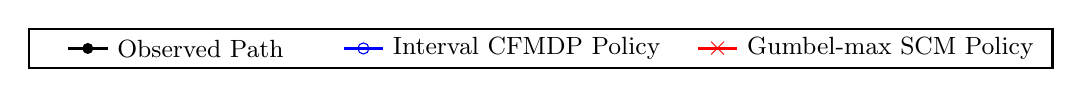
\begin{tikzpicture}[scale=1.0, every node/.style={scale=1.0}]
            \draw[thick, black] (-3, -0.25) rectangle (10, 0.25);
            %
            \draw[black, line width=1pt] (-2.5, 0.0) -- (-2,0.0);
            \fill[black] (-2.25,0.0) circle (2pt); %
            \node[right] at (-2,0.0) {\small Observed Path};
            
            %
            \draw[blue, line width=1pt] (1.0,0.0) -- (1.5,0.0);
            \node[draw=blue, circle, minimum size=4pt, inner sep=0pt] at (1.25,0.0) {}; %
            \node[right] at (1.5,0.0) {\small Interval CFMDP Policy};
            
            %
            \draw[red, line width=1pt] (5.5,0) -- (6,0);
            \node[red] at (5.75,0) {$\boldsymbol{\times}$}; %
            \node[right] at (6,0) {\small Gumbel-max SCM Policy};
        \end{tikzpicture}
    }\\
    %
    \subfigure[\footnotesize Lowest cumulative reward: Interval CFMDP ($312$), Gumbel-max SCM ($312$)]{%
        \resizebox{0.76\columnwidth}{!}{
             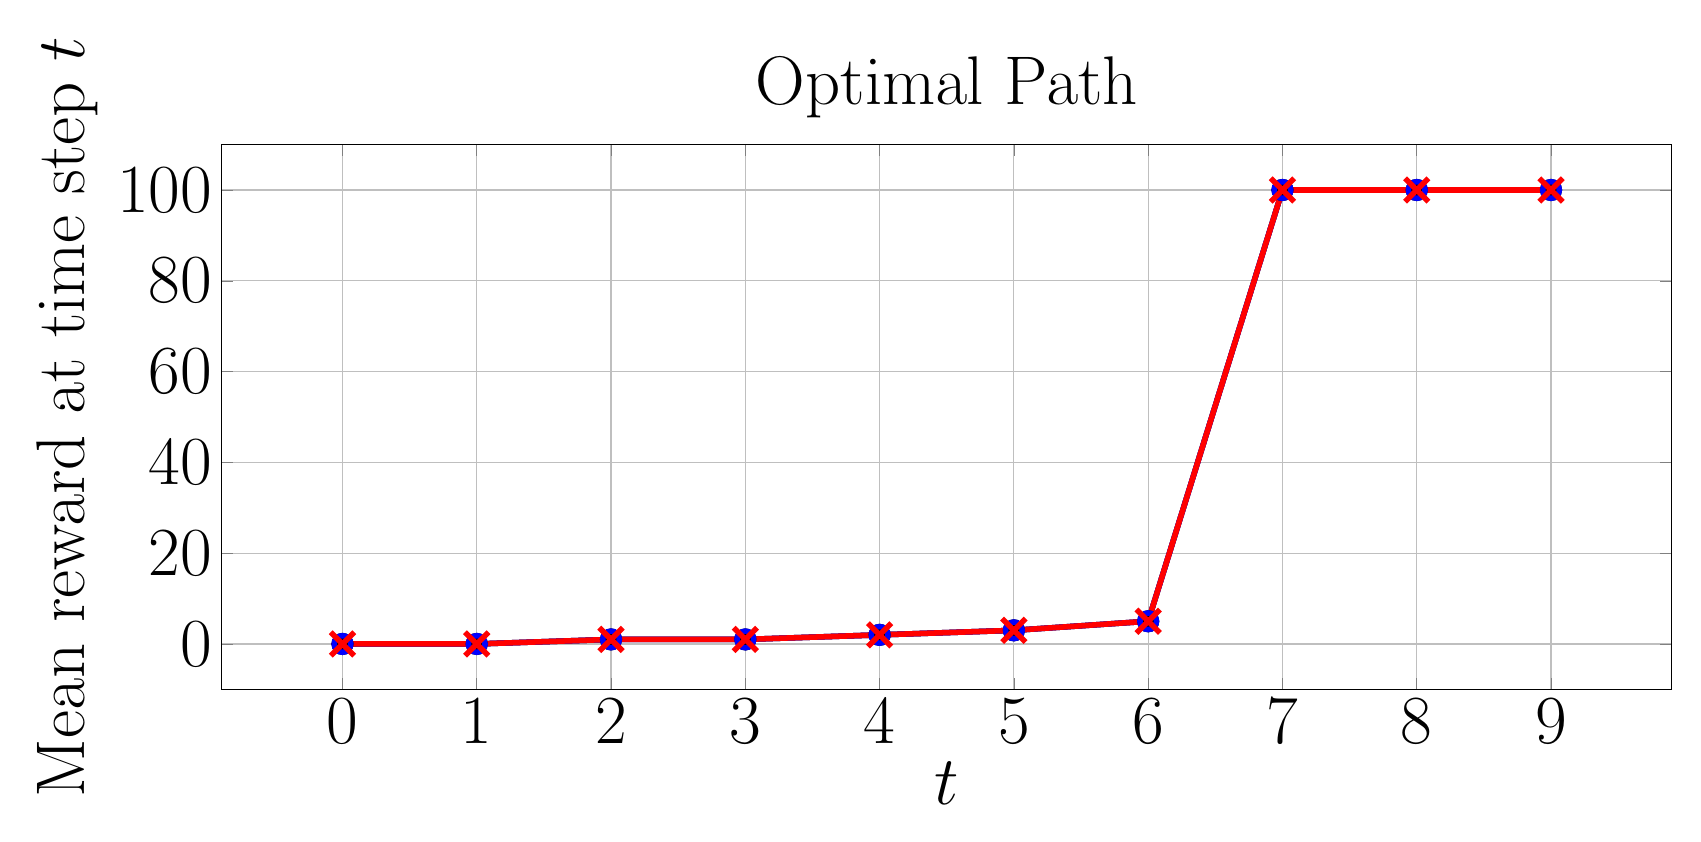
\begin{tikzpicture}
                \begin{axis}[
                    xlabel={$t$},
                    ylabel={Mean reward at time step $t$},
                    title={Optimal Path},
                    grid=both,
                    width=20cm, height=8.5cm,
                    every axis/.style={font=\Huge},
                    %
                ]
                \addplot[
                    color=black, %
                    mark=*, %
                    line width=2pt,
                    mark size=3pt,
                    error bars/.cd,
                    y dir=both, %
                    y explicit, %
                    error bar style={line width=1pt,solid},
                    error mark options={line width=1pt,mark size=4pt,rotate=90}
                ]
                coordinates {
                    (0, 0.0)  +- (0, 0.0)
                    (1, 0.0)  +- (0, 0.0) 
                    (2, 1.0)  +- (0, 0.0) 
                    (3, 1.0)  +- (0, 0.0)
                    (4, 2.0)  +- (0, 0.0)
                    (5, 3.0) +- (0, 0.0)
                    (6, 5.0) +- (0, 0.0)
                    (7, 100.0) +- (0, 0.0)
                    (8, 100.0) +- (0, 0.0)
                    (9, 100.0) +- (0, 0.0)
                };
                %
                \addplot[
                    color=blue, %
                    mark=o, %
                    line width=2pt,
                    mark size=3pt,
                    error bars/.cd,
                    y dir=both, %
                    y explicit, %
                    error bar style={line width=1pt,solid},
                    error mark options={line width=1pt,mark size=4pt,rotate=90}
                ]
                 coordinates {
                    (0, 0.0)  +- (0, 0.0)
                    (1, 0.0)  +- (0, 0.0) 
                    (2, 1.0)  +- (0, 0.0) 
                    (3, 1.0)  +- (0, 0.0)
                    (4, 2.0)  +- (0, 0.0)
                    (5, 3.0) +- (0, 0.0)
                    (6, 5.0) +- (0, 0.0)
                    (7, 100.0) +- (0, 0.0)
                    (8, 100.0) +- (0, 0.0)
                    (9, 100.0) +- (0, 0.0)
                };
                %
                \addplot[
                    color=red, %
                    mark=x, %
                    line width=2pt,
                    mark size=6pt,
                    error bars/.cd,
                    y dir=both, %
                    y explicit, %
                    error bar style={line width=1pt,solid},
                    error mark options={line width=1pt,mark size=4pt,rotate=90}
                ]
                coordinates {
                    (0, 0.0)  +- (0, 0.0)
                    (1, 0.0)  +- (0, 0.0) 
                    (2, 1.0)  +- (0, 0.0) 
                    (3, 1.0)  +- (0, 0.0)
                    (4, 2.0)  +- (0, 0.0)
                    (5, 3.0) +- (0, 0.0)
                    (6, 5.0) +- (0, 0.0)
                    (7, 100.0) +- (0, 0.0)
                    (8, 100.0) +- (0, 0.0)
                    (9, 100.0) +- (0, 0.0)
                };
                \end{axis}
            \end{tikzpicture}
         }
    }
    \hspace{1cm}
    \subfigure[\footnotesize Lowest cumulative reward: Interval CFMDP ($19$), Gumbel-max SCM ($-88$)]{%
         \resizebox{0.76\columnwidth}{!}{
            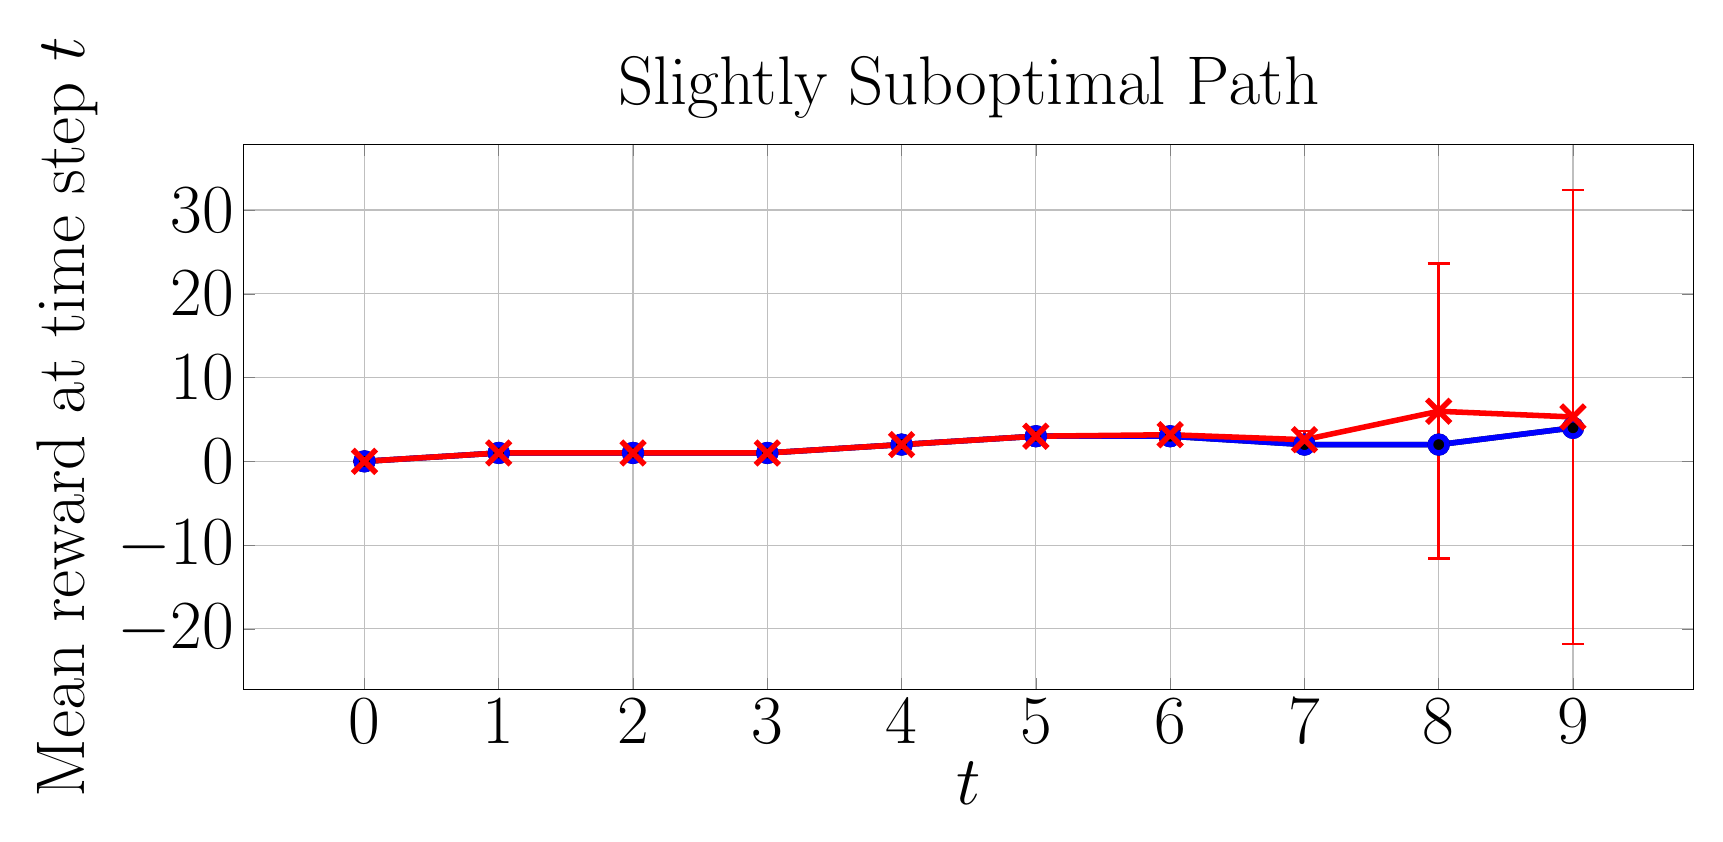
\begin{tikzpicture}
                \begin{axis}[
                    xlabel={$t$},
                    ylabel={Mean reward at time step $t$},
                    title={Slightly Suboptimal Path},
                    grid=both,
                    width=20cm, height=8.5cm,
                    every axis/.style={font=\Huge},
                    %
                ]
                \addplot[
                    color=black, %
                    mark=*, %
                    line width=2pt,
                    mark size=3pt,
                    error bars/.cd,
                    y dir=both, %
                    y explicit, %
                    error bar style={line width=1pt,solid},
                    error mark options={line width=1pt,mark size=4pt,rotate=90}
                ]
              coordinates {
                    (0, 0.0)  +- (0, 0.0)
                    (1, 1.0)  +- (0, 0.0) 
                    (2, 1.0)  +- (0, 0.0) 
                    (3, 1.0)  +- (0, 0.0)
                    (4, 2.0)  +- (0, 0.0)
                    (5, 3.0) +- (0, 0.0)
                    (6, 3.0) +- (0, 0.0)
                    (7, 2.0) +- (0, 0.0)
                    (8, 2.0) +- (0, 0.0)
                    (9, 4.0) +- (0, 0.0)
                };
                %
                \addplot[
                    color=blue, %
                    mark=o, %
                    line width=2pt,
                    mark size=3pt,
                    error bars/.cd,
                    y dir=both, %
                    y explicit, %
                    error bar style={line width=1pt,solid},
                    error mark options={line width=1pt,mark size=4pt,rotate=90}
                ]
              coordinates {
                    (0, 0.0)  +- (0, 0.0)
                    (1, 1.0)  +- (0, 0.0) 
                    (2, 1.0)  +- (0, 0.0) 
                    (3, 1.0)  +- (0, 0.0)
                    (4, 2.0)  +- (0, 0.0)
                    (5, 3.0) +- (0, 0.0)
                    (6, 3.0) +- (0, 0.0)
                    (7, 2.0) +- (0, 0.0)
                    (8, 2.0) +- (0, 0.0)
                    (9, 4.0) +- (0, 0.0)
                };
                %
                \addplot[
                    color=red, %
                    mark=x, %
                    line width=2pt,
                    mark size=6pt,
                    error bars/.cd,
                    y dir=both, %
                    y explicit, %
                    error bar style={line width=1pt,solid},
                    error mark options={line width=1pt,mark size=4pt,rotate=90}
                ]
                coordinates {
                    (0, 0.0)  +- (0, 0.0)
                    (1, 1.0)  +- (0, 0.0) 
                    (2, 1.0)  +- (0, 0.0) 
                    (3, 1.0)  +- (0, 0.0)
                    (4, 2.0)  += (0, 0.0)
                    (5, 3.0)  += (0, 0.0)
                    (6, 3.17847) += (0, 0.62606746) -= (0, 0.62606746)
                    (7, 2.5832885) += (0, 1.04598233) -= (0, 1.04598233)
                    (8, 5.978909) += (0, 17.60137623) -= (0, 17.60137623)
                    (9, 5.297059) += (0, 27.09227512) -= (0, 27.09227512)
                };
                \end{axis}
            \end{tikzpicture}
         }
    }\\[-1.5pt]
    \subfigure[\footnotesize Lowest cumulative reward: Interval CFMDP ($14$), Gumbel-max SCM ($-598$)]{%
         \resizebox{0.76\columnwidth}{!}{
             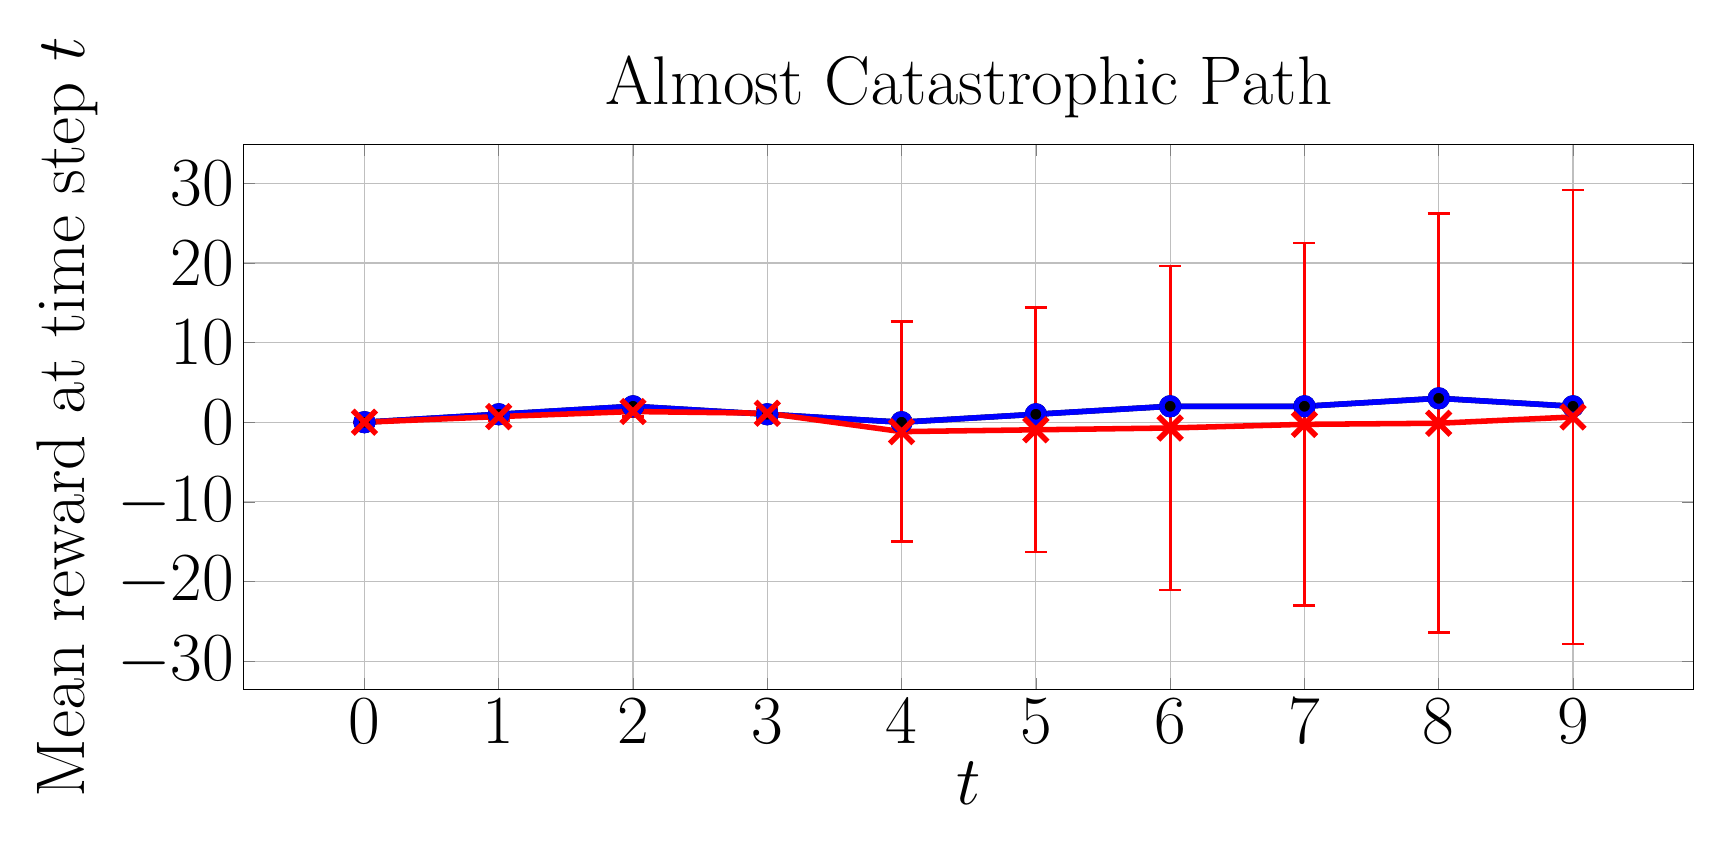
\begin{tikzpicture}
                \begin{axis}[
                    xlabel={$t$},
                    ylabel={Mean reward at time step $t$},
                    title={Almost Catastrophic Path},
                    grid=both,
                    width=20cm, height=8.5cm,
                    every axis/.style={font=\Huge},
                    %
                ]
                \addplot[
                    color=black, %
                    mark=*, %
                    line width=2pt,
                    mark size=3pt,
                    error bars/.cd,
                    y dir=both, %
                    y explicit, %
                    error bar style={line width=1pt,solid},
                    error mark options={line width=1pt,mark size=4pt,rotate=90}
                ]
                coordinates {
                    (0, 0.0)  +- (0, 0.0)
                    (1, 1.0)  +- (0, 0.0) 
                    (2, 2.0)  +- (0, 0.0) 
                    (3, 1.0)  +- (0, 0.0)
                    (4, 0.0)  +- (0, 0.0)
                    (5, 1.0) +- (0, 0.0)
                    (6, 2.0) +- (0, 0.0)
                    (7, 2.0) +- (0, 0.0)
                    (8, 3.0) +- (0, 0.0)
                    (9, 2.0) +- (0, 0.0)
                };
                %
                \addplot[
                    color=blue, %
                    mark=o, %
                    line width=2pt,
                    mark size=3pt,
                    error bars/.cd,
                    y dir=both, %
                    y explicit, %
                    error bar style={line width=1pt,solid},
                    error mark options={line width=1pt,mark size=4pt,rotate=90}
                ]
                coordinates {
                    (0, 0.0)  +- (0, 0.0)
                    (1, 1.0)  +- (0, 0.0) 
                    (2, 2.0)  +- (0, 0.0) 
                    (3, 1.0)  +- (0, 0.0)
                    (4, 0.0)  +- (0, 0.0)
                    (5, 1.0) +- (0, 0.0)
                    (6, 2.0) +- (0, 0.0)
                    (7, 2.0) +- (0, 0.0)
                    (8, 3.0) +- (0, 0.0)
                    (9, 2.0) +- (0, 0.0)
                };
                %
                \addplot[
                    color=red, %
                    mark=x, %
                    line width=2pt,
                    mark size=6pt,
                    error bars/.cd,
                    y dir=both, %
                    y explicit, %
                    error bar style={line width=1pt,solid},
                    error mark options={line width=1pt,mark size=4pt,rotate=90}
                ]
                coordinates {
                    (0, 0.0)  +- (0, 0.0)
                    (1, 0.7065655)  +- (0, 0.4553358) 
                    (2, 1.341673)  +- (0, 0.67091621) 
                    (3, 1.122926)  +- (0, 0.61281824)
                    (4, -1.1821935)  +- (0, 13.82444042)
                    (5, -0.952399)  +- (0, 15.35195457)
                    (6, -0.72672) +- (0, 20.33508414)
                    (7, -0.268983) +- (0, 22.77861454)
                    (8, -0.1310835) +- (0, 26.31013314)
                    (9, 0.65806) +- (0, 28.50670214)
                };
                %
            %
            %
            %
            %
            %
            %
            %
            %
            %
            %
            %
            %
            %
            %
            %
            %
            %
            %
                \end{axis}
            \end{tikzpicture}
         }
    }
    \hspace{1cm}
    \subfigure[\footnotesize Lowest cumulative reward: Interval CFMDP ($-698$), Gumbel-max SCM ($-698$)]{%
         \resizebox{0.76\columnwidth}{!}{
            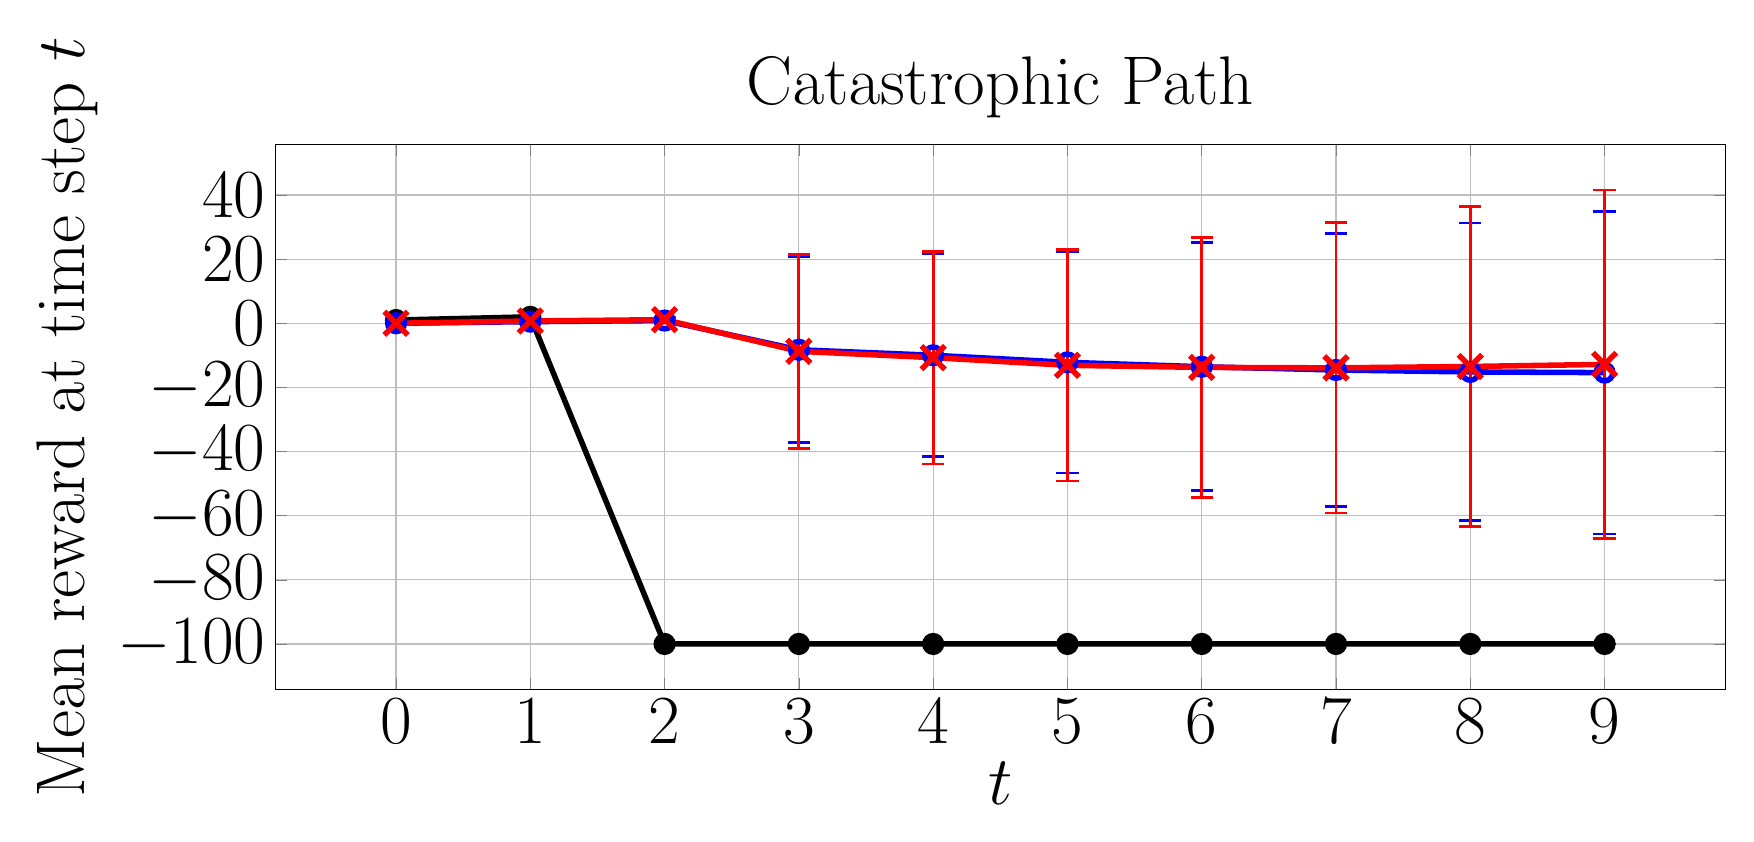
\begin{tikzpicture}
                \begin{axis}[
                    xlabel={$t$},
                    ylabel={Mean reward at time step $t$},
                    title={Catastrophic Path},
                    grid=both,
                    width=20cm, height=8.5cm,
                    every axis/.style={font=\Huge},
                    %
                ]
                \addplot[
                    color=black, %
                    mark=*, %
                    line width=2pt,
                    mark size=3pt,
                    error bars/.cd,
                    y dir=both, %
                    y explicit, %
                    error bar style={line width=1pt,solid},
                    error mark options={line width=1pt,mark size=4pt,rotate=90}
                ]
                coordinates {
                    (0, 1.0)  +- (0, 0.0)
                    (1, 2.0)  +- (0, 0.0) 
                    (2, -100.0)  +- (0, 0.0) 
                    (3, -100.0)  +- (0, 0.0)
                    (4, -100.0)  +- (0, 0.0)
                    (5, -100.0) +- (0, 0.0)
                    (6, -100.0) +- (0, 0.0)
                    (7, -100.0) +- (0, 0.0)
                    (8, -100.0) +- (0, 0.0)
                    (9, -100.0) +- (0, 0.0)
                };
                %
                \addplot[
                    color=blue, %
                    mark=o, %
                    line width=2pt,
                    mark size=3pt,
                    error bars/.cd,
                    y dir=both, %
                    y explicit, %
                    error bar style={line width=1pt,solid},
                    error mark options={line width=1pt,mark size=4pt,rotate=90}
                ]
                coordinates {
                    (0, 0.0)  +- (0, 0.0)
                    (1, 0.504814)  +- (0, 0.49997682) 
                    (2, 0.8439835)  +- (0, 0.76831917) 
                    (3, -8.2709165)  +- (0, 28.93656754)
                    (4, -9.981082)  +- (0, 31.66825363)
                    (5, -12.1776325) +- (0, 34.53463233)
                    (6, -13.556076) +- (0, 38.62845372)
                    (7, -14.574418) +- (0, 42.49603359)
                    (8, -15.1757075) +- (0, 46.41913968)
                    (9, -15.3900395) +- (0, 50.33563368)
                };
                %
                \addplot[
                    color=red, %
                    mark=x, %
                    line width=2pt,
                    mark size=6pt,
                    error bars/.cd,
                    y dir=both, %
                    y explicit, %
                    error bar style={line width=1pt,solid},
                    error mark options={line width=1pt,mark size=4pt,rotate=90}
                ]
                coordinates {
                    (0, 0.0)  +- (0, 0.0)
                    (1, 0.701873)  +- (0, 0.45743556) 
                    (2, 1.1227805)  +- (0, 0.73433129) 
                    (3, -8.7503255)  +- (0, 30.30257976)
                    (4, -10.722092)  +- (0, 33.17618589)
                    (5, -13.10721)  +- (0, 36.0648089)
                    (6, -13.7631645) +- (0, 40.56553451)
                    (7, -13.909043) +- (0, 45.23829402)
                    (8, -13.472517) +- (0, 49.96270296)
                    (9, -12.8278835) +- (0, 54.38618735)
                };
                %
            %
            %
            %
            %
            %
            %
            %
            %
            %
            %
            %
            %
            %
            %
            %
            %
            %
            %
                \end{axis}
            \end{tikzpicture}
         }
    }
    \caption{Average instant reward of CF paths induced by policies on GridWorld $p=0.4$.}
    \label{fig: reward p=0.4}
\end{figure*}

\subsection{Experimental Setup}
To compare policy performance, we measure the average rewards of counterfactual paths induced by our policy and the Gumbel-max policy by uniformly sampling $200$ counterfactual MDPs from the ICFMDP and generating $10,000$ counterfactual paths over each sampled CFMDP. \jl{Since the interval CFMDP depends on the observed path, we select $4$  paths of varying optimality to evaluate how the observed path impacts the performance of both policies: an optimal path, a slightly suboptimal path that could reach the optimal reward with a few changes, a catastrophic path that enters a catastrophic, terminal state with low reward, and an almost catastrophic path that was close to entering a catastrophic state.} When measuring the average probability bound widths and execution time needed to generate the ICFMDPs, we averaged over $20$ randomly generated observed paths
\footnote{Further training details are provided in Appendix \ref{app: training details}, and the code is provided at \href{https://github.com/ddv-lab/robust-cf-inference-in-MDPs}{https://github.com/ddv-lab/robust-cf-inference-in-MDPs}
%
%
.}.

\subsection{GridWorld}
\jl{The GridWorld MDP is a $4 \times 4$ grid where an agent must navigate from the top-left corner to the goal state in the bottom-right corner, avoiding a dangerous terminal state in the centre. At each time step, the agent can move up, down, left, or right, but there is a small probability (controlled by hyper-parameter $p$) of moving in an unintended direction. As the agent nears the goal, the reward for each state increases, culminating in a reward of $+100$ for reaching the goal. Entering the dangerous state results in a penalty of $-100$. We use two versions of GridWorld: a less stochastic version with $p=0.9$ (i.e., $90$\% chance of moving in the chosen direction) and a more stochastic version with $p=0.4$.}

\paragraph{GridWorld ($p=0.9$)}
When $p=0.9$, the counterfactual probability bounds are typically narrow (see Table \ref{tab:nonzero_probs} for average measurements). Consequently, as shown in Figure \ref{fig: reward p=0.9}, both policies are nearly identical and perform similarly well across the optimal, slightly suboptimal, and catastrophic paths.
%
However, for the almost catastrophic path, the interval CFMDP path is more conservative and follows the observed path more closely (as this is where the probability bounds are narrowest), which typically requires one additional step to reach the goal state than the Gumbel-max SCM policy.
%

\paragraph{GridWorld ($p=0.4$)}
\jl{When $p=0.4$, the GridWorld environment becomes more uncertain, increasing the risk of entering the dangerous state even if correct actions are chosen. Thus, as shown in Figure \ref{fig: reward p=0.4}, the interval CFMDP policy adopts a more conservative approach, avoiding deviation from the observed policy if it cannot guarantee higher counterfactual rewards (see the slightly suboptimal and almost catastrophic paths), whereas the Gumbel-max SCM is inconsistent: it can yield higher rewards, but also much lower rewards, reflected in the wide error bars.} For the catastrophic path, both policies must deviate from the observed path to achieve a higher reward and, in this case, perform similarly.
%
%
%
%
\subsection{Sepsis}
The Sepsis MDP \citep{oberst2019counterfactual} simulates trajectories of Sepsis patients. Each state consists of four vital signs (heart rate, blood pressure, oxygen concentration, and glucose levels), categorised as low, normal, or high.
and three treatments that can be toggled on/off at each time step (8 actions in total). Unlike \citet{oberst2019counterfactual}, we scale rewards based on the number of out-of-range vital signs, between $-1000$ (patient dies) and $1000$ (patient discharged). \jl{Like the GridWorld $p=0.4$ experiment, the Sepsis MDP is highly uncertain, as many states are equally likely to lead to optimal and poor outcomes. Thus, as shown in Figure \ref{fig: reward sepsis}, both policies follow the observed optimal and almost catastrophic paths to guarantee rewards are no worse than the observation.} However, improving the catastrophic path requires deviating from the observation. Here, the Gumbel-max SCM policy, on average, performs better than the interval CFMDP policy. But, since both policies have lower bounds clipped at $-1000$, neither policy reliably improves over the observation. In contrast, for the slightly suboptimal path, the interval CFMDP policy performs significantly better, shown by its higher lower bounds. 
Moreover, in these two cases, the worst-case counterfactual path generated by the interval CFMDP policy is better than that of the Gumbel-max SCM policy,
indicating its greater robustness.
%
\begin{figure*}
    \centering
     \resizebox{0.6\textwidth}{!}{
        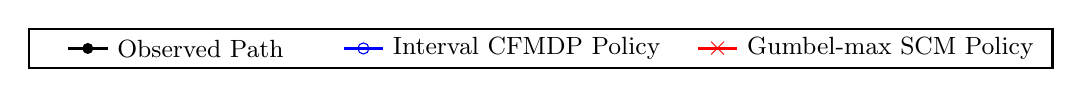
\begin{tikzpicture}[scale=1.0, every node/.style={scale=1.0}]
            \draw[thick, black] (-3, -0.25) rectangle (10, 0.25);
            %
            \draw[black, line width=1pt] (-2.5, 0.0) -- (-2,0.0);
            \fill[black] (-2.25,0.0) circle (2pt); %
            \node[right] at (-2,0.0) {\small Observed Path};
            
            %
            \draw[blue, line width=1pt] (1.0,0.0) -- (1.5,0.0);
            \node[draw=blue, circle, minimum size=4pt, inner sep=0pt] at (1.25,0.0) {}; %
            \node[right] at (1.5,0.0) {\small Interval CFMDP Policy};
            
            %
            \draw[red, line width=1pt] (5.5,0) -- (6,0);
            \node[red] at (5.75,0) {$\boldsymbol{\times}$}; %
            \node[right] at (6,0) {\small Gumbel-max SCM Policy};
        \end{tikzpicture}
    }\\
    \subfigure[\footnotesize Lowest cumulative reward: Interval CFMDP ($8000$), Gumbel-max SCM ($8000$)]{%
         \resizebox{0.76\columnwidth}{!}{
             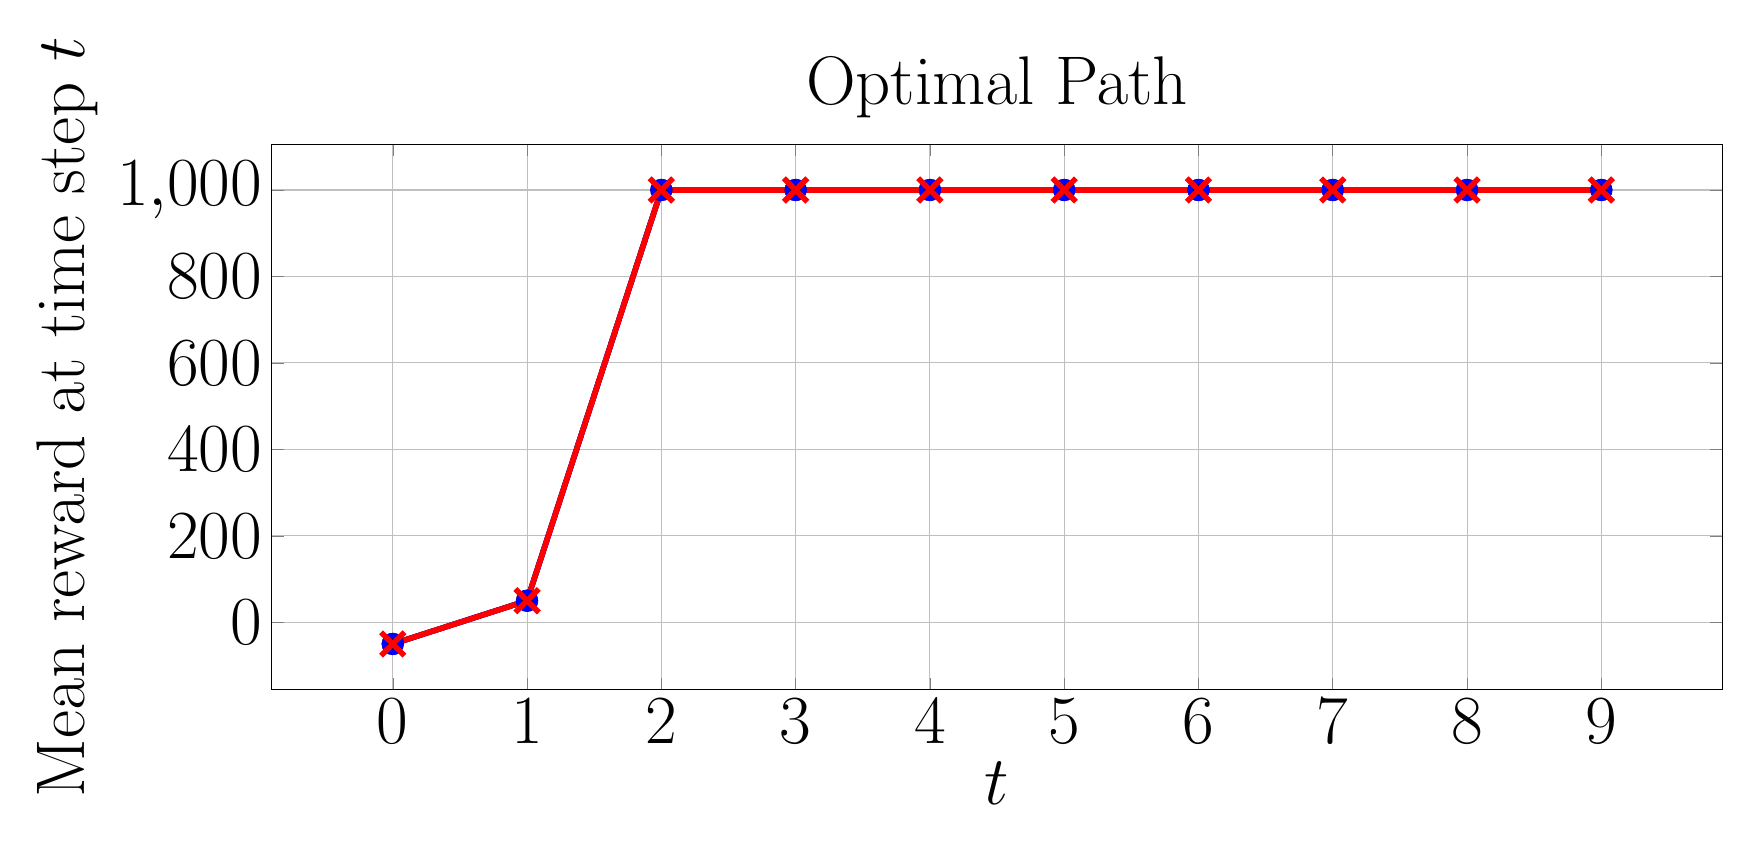
\begin{tikzpicture}
                \begin{axis}[
                    xlabel={$t$},
                    ylabel={Mean reward at time step $t$},
                    title={Optimal Path},
                    grid=both,
                    width=20cm, height=8.5cm,
                    every axis/.style={font=\Huge},
                    %
                ]
                \addplot[
                    color=black, %
                    mark=*, %
                    line width=2pt,
                    mark size=3pt,
                ]
                coordinates {
                    (0, -50.0)
                    (1, 50.0)
                    (2, 1000.0)
                    (3, 1000.0)
                    (4, 1000.0)
                    (5, 1000.0)
                    (6, 1000.0)
                    (7, 1000.0)
                    (8, 1000.0)
                    (9, 1000.0)
                };
                %
                \addplot[
                    color=blue, %
                    mark=o, %
                    line width=2pt,
                    mark size=3pt,
                    error bars/.cd,
                    y dir=both, %
                    y explicit, %
                    error bar style={line width=1pt,solid},
                    error mark options={line width=1pt,mark size=4pt,rotate=90}
                ]
                coordinates {
                    (0, -50.0)  +- (0, 0.0)
                    (1, 50.0)  +- (0, 0.0) 
                    (2, 1000.0)  +- (0, 0.0) 
                    (3, 1000.0)  +- (0, 0.0)
                    (4, 1000.0)  +- (0, 0.0)
                    (5, 1000.0) +- (0, 0.0)
                    (6, 1000.0) +- (0, 0.0)
                    (7, 1000.0) +- (0, 0.0)
                    (8, 1000.0) +- (0, 0.0)
                    (9, 1000.0) +- (0, 0.0)
                };
                %
                \addplot[
                    color=red, %
                    mark=x, %
                    line width=2pt,
                    mark size=6pt,
                    error bars/.cd,
                    y dir=both, %
                    y explicit, %
                    error bar style={line width=1pt,solid},
                    error mark options={line width=1pt,mark size=4pt,rotate=90}
                ]
                coordinates {
                    (0, -50.0)  +- (0, 0.0)
                    (1, 50.0)  +- (0, 0.0) 
                    (2, 1000.0)  +- (0, 0.0) 
                    (3, 1000.0)  +- (0, 0.0)
                    (4, 1000.0)  +- (0, 0.0)
                    (5, 1000.0) +- (0, 0.0)
                    (6, 1000.0) +- (0, 0.0)
                    (7, 1000.0) +- (0, 0.0)
                    (8, 1000.0) +- (0, 0.0)
                    (9, 1000.0) +- (0, 0.0)
                };
                %
                \end{axis}
            \end{tikzpicture}
         }
    }
    \hspace{1cm}
    \subfigure[\footnotesize Lowest cumulative reward: Interval CFMDP ($-5980$), Gumbel-max SCM ($-8000$)]{%
         \resizebox{0.76\columnwidth}{!}{
            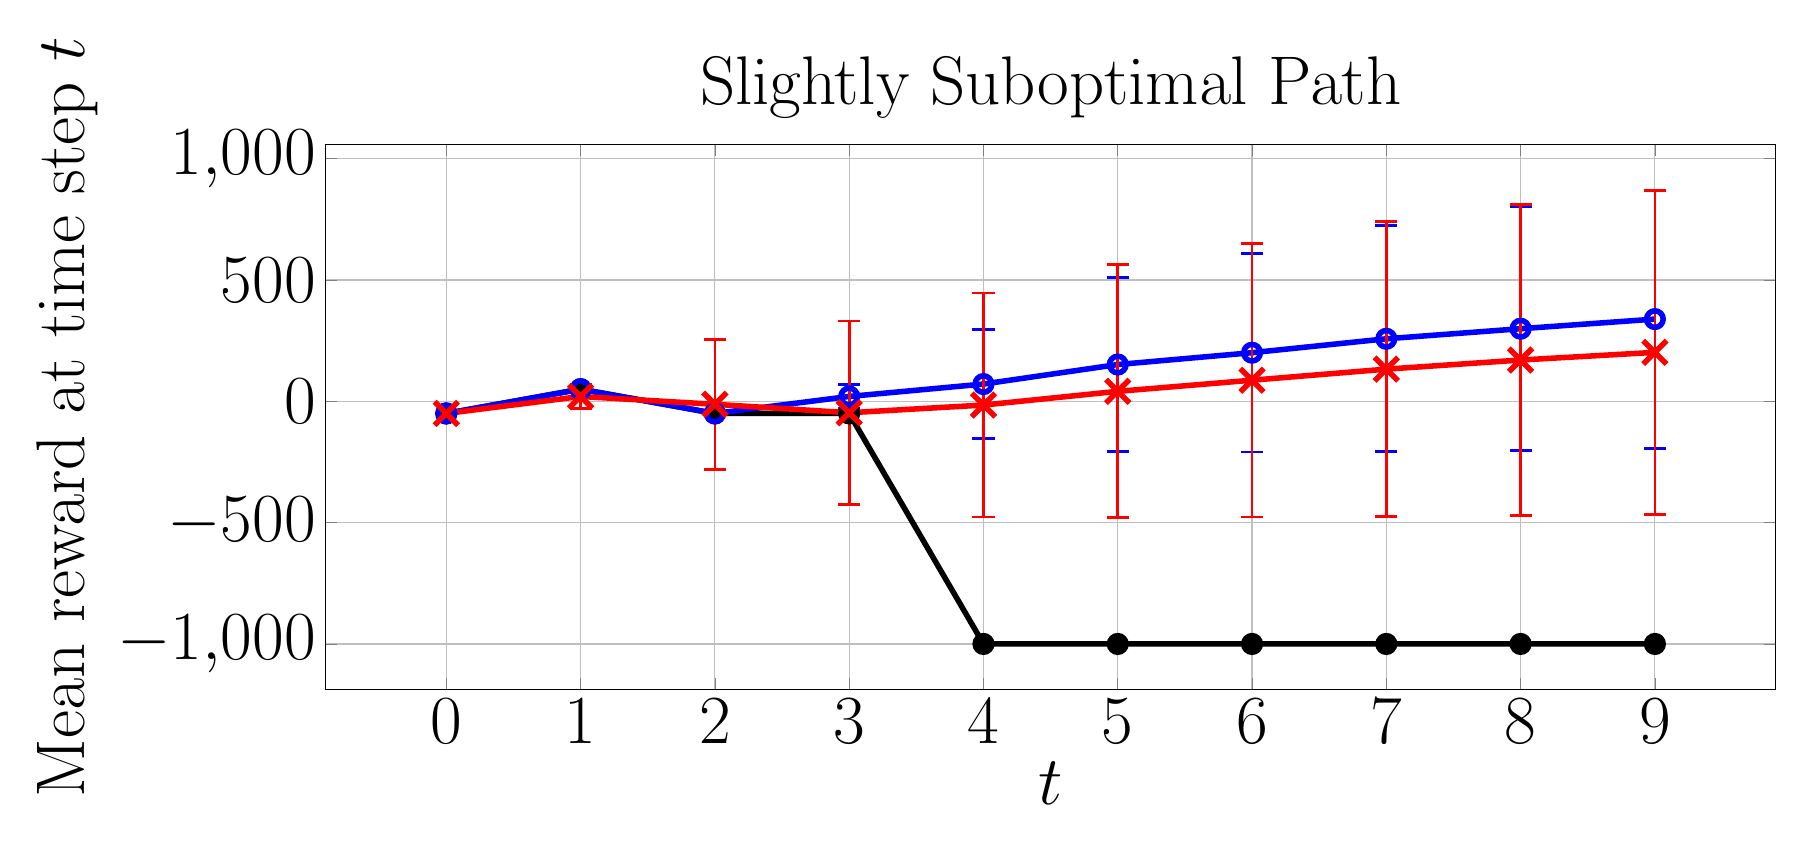
\begin{tikzpicture}
                \begin{axis}[
                    xlabel={$t$},
                    ylabel={Mean reward at time step $t$},
                    title={Slightly Suboptimal Path},
                    grid=both,
                    width=20cm, height=8.5cm,
                    every axis/.style={font=\Huge},
                    %
                ]
               \addplot[
                    color=black, %
                    mark=*, %
                    line width=2pt,
                    mark size=3pt,
                ]
                coordinates {
                    (0, -50.0)
                    (1, 50.0)
                    (2, -50.0)
                    (3, -50.0)
                    (4, -1000.0)
                    (5, -1000.0)
                    (6, -1000.0)
                    (7, -1000.0)
                    (8, -1000.0)
                    (9, -1000.0)
                };
                %
                \addplot[
                    color=blue, %
                    mark=o, %
                    line width=2pt,
                    mark size=3pt,
                    error bars/.cd,
                    y dir=both, %
                    y explicit, %
                    error bar style={line width=1pt,solid},
                    error mark options={line width=1pt,mark size=4pt,rotate=90}
                ]
                coordinates {
                    (0, -50.0)  +- (0, 0.0)
                    (1, 50.0)  +- (0, 0.0) 
                    (2, -50.0)  +- (0, 0.0) 
                    (3, 20.0631)  +- (0, 49.97539413)
                    (4, 71.206585)  +- (0, 226.02033693)
                    (5, 151.60797) +- (0, 359.23292559)
                    (6, 200.40593) +- (0, 408.86185176)
                    (7, 257.77948) +- (0, 466.10372804)
                    (8, 299.237465) +- (0, 501.82579506)
                    (9, 338.9129) +- (0, 532.06124996)
                };
                %
                \addplot[
                    color=red, %
                    mark=x, %
                    line width=2pt,
                    mark size=6pt,
                    error bars/.cd,
                    y dir=both, %
                    y explicit, %
                    error bar style={line width=1pt,solid},
                    error mark options={line width=1pt,mark size=4pt,rotate=90}
                ]
                coordinates {
                    (0, -50.0)  +- (0, 0.0)
                    (1, 20.00736)  +- (0, 49.99786741) 
                    (2, -12.282865)  +- (0, 267.598755) 
                    (3, -47.125995)  +- (0, 378.41755832)
                    (4, -15.381965)  +- (0, 461.77616558)
                    (5, 41.15459) +- (0, 521.53189262)
                    (6, 87.01595) +- (0, 564.22243126 )
                    (7, 132.62376) +- (0, 607.31338037)
                    (8, 170.168145) +- (0, 641.48013693)
                    (9, 201.813135) +- (0, 667.29441777)
                };
                %
                %
                %
                %
                %
                %
                %
                %
                %
                %
                %
                %
                %
                %
                %
                %
                %
                %
                %
                \end{axis}
            \end{tikzpicture}
         }
    }\\[-1.5pt]
    \subfigure[\footnotesize Lowest cumulative reward: Interval CFMDP ($100$), Gumbel-max SCM ($100$)]{%
         \resizebox{0.76\columnwidth}{!}{
             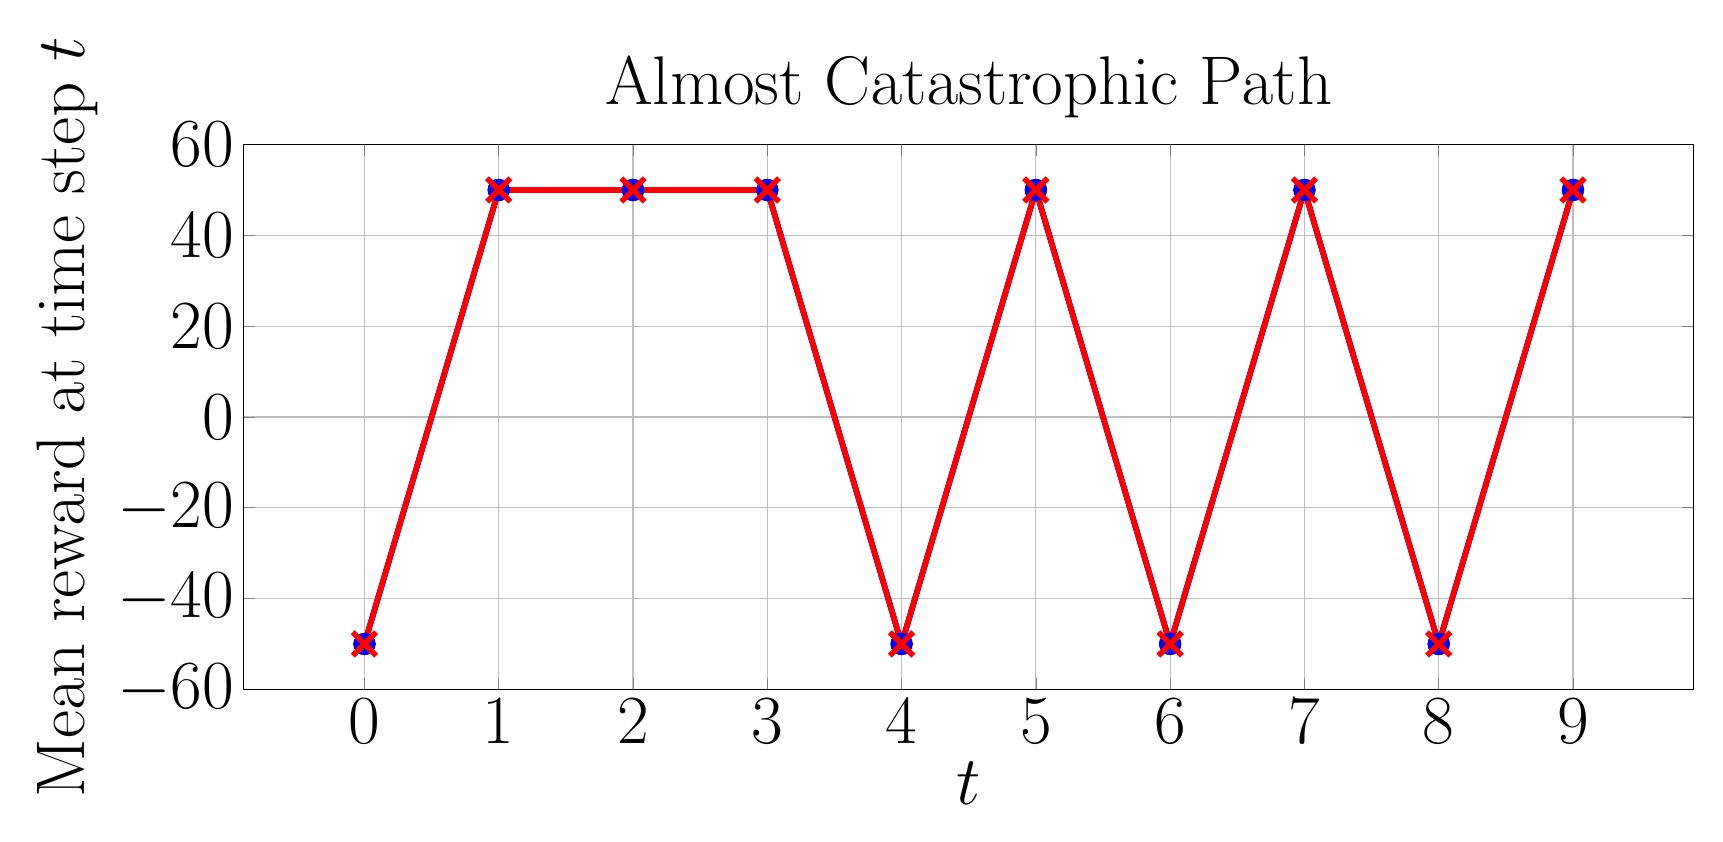
\begin{tikzpicture}
                \begin{axis}[
                    xlabel={$t$},
                    ylabel={Mean reward at time step $t$},
                    title={Almost Catastrophic Path},
                    grid=both,
                    every axis/.style={font=\Huge},
                    width=20cm, height=8.5cm,
                    %
                ]
               \addplot[
                    color=black, %
                    mark=*, %
                    line width=2pt,
                    mark size=3pt,
                ]
                coordinates {
                    (0, -50.0)
                    (1, 50.0)
                    (2, 50.0)
                    (3, 50.0)
                    (4, -50.0)
                    (5, 50.0)
                    (6, -50.0)
                    (7, 50.0)
                    (8, -50.0)
                    (9, 50.0)
                };
                %
                %
                \addplot[
                    color=blue, %
                    mark=o, %
                    line width=2pt,
                    mark size=3pt,
                    error bars/.cd,
                    y dir=both, %
                    y explicit, %
                    error bar style={line width=1pt,solid},
                    error mark options={line width=1pt,mark size=4pt,rotate=90}
                ]
                coordinates {
                    (0, -50.0)  +- (0, 0.0)
                    (1, 50.0)  +- (0, 0.0) 
                    (2, 50.0)  +- (0, 0.0) 
                    (3, 50.0)  +- (0, 0.0)
                    (4, -50.0)  +- (0, 0.0)
                    (5, 50.0) +- (0, 0.0)
                    (6, -50.0) +- (0, 0.0)
                    (7, 50.0) +- (0, 0.0)
                    (8, -50.0) +- (0, 0.0)
                    (9, 50.0) +- (0, 0.0)
                };
                %
                \addplot[
                    color=red, %
                    mark=x, %
                    line width=2pt,
                    mark size=6pt,
                    error bars/.cd,
                    y dir=both, %
                    y explicit, %
                    error bar style={line width=1pt,solid},
                    error mark options={line width=1pt,mark size=4pt,rotate=90}
                ]
                coordinates {
                    (0, -50.0)  +- (0, 0.0)
                    (1, 50.0)  +- (0, 0.0) 
                    (2, 50.0)  +- (0, 0.0) 
                    (3, 50.0)  +- (0, 0.0)
                    (4, -50.0)  +- (0, 0.0)
                    (5, 50.0) +- (0, 0.0)
                    (6, -50.0) +- (0, 0.0)
                    (7, 50.0) +- (0, 0.0)
                    (8, -50.0) +- (0, 0.0)
                    (9, 50.0) +- (0, 0.0)
                };
                %
                %
                %
                %
                %
                %
                %
                %
                %
                %
                %
                %
                %
                %
                %
                %
                %
                %
                %
                \end{axis}
            \end{tikzpicture}
         }
    }
    \hspace{1cm}
    \subfigure[\footnotesize Lowest cumulative reward: Interval CFMDP ($-7150$), Gumbel-max SCM ($-9050$)]{%
         \resizebox{0.76\columnwidth}{!}{
            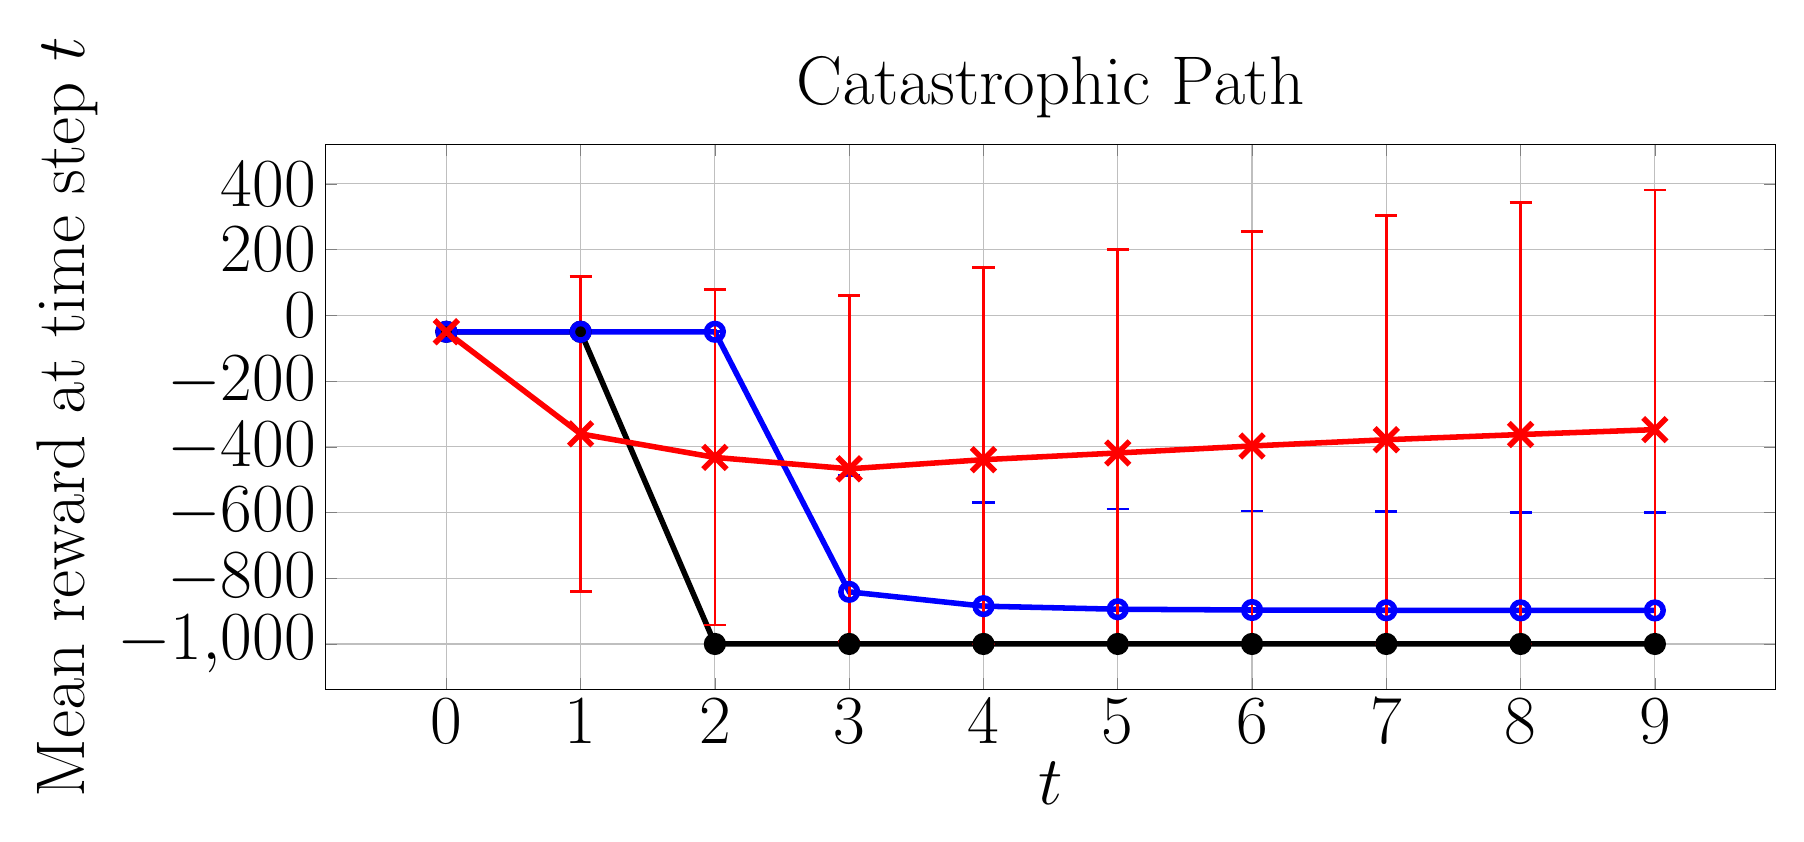
\begin{tikzpicture}
                \begin{axis}[
                    xlabel={$t$},
                    ylabel={Mean reward at time step $t$},
                    title={Catastrophic Path},
                    grid=both,
                    width=20cm, height=8.5cm,
                    every axis/.style={font=\Huge},
                    %
                ]
               \addplot[
                    color=black, %
                    mark=*, %
                    line width=2pt,
                    mark size=3pt,
                ]
                coordinates {
                    (0, -50.0)
                    (1, -50.0)
                    (2, -1000.0)
                    (3, -1000.0)
                    (4, -1000.0)
                    (5, -1000.0)
                    (6, -1000.0)
                    (7, -1000.0)
                    (8, -1000.0)
                    (9, -1000.0)
                };
                %
                %
                \addplot[
                    color=blue, %
                    mark=o, %
                    line width=2pt,
                    mark size=3pt,
                    error bars/.cd,
                    y dir=both, %
                    y explicit, %
                    error bar style={line width=1pt,solid},
                    error mark options={line width=1pt,mark size=4pt,rotate=90}
                ]
                coordinates {
                    (0, -50.0)  +- (0, 0.0)
                    (1, -50.0)  +- (0, 0.0) 
                    (2, -50.0)  +- (0, 0.0) 
                    (3, -841.440725)  += (0, 354.24605512) -= (0, 158.559275)
                    (4, -884.98225)  += (0, 315.37519669) -= (0, 115.01775)
                    (5, -894.330425) += (0, 304.88572805) -= (0, 105.669575)
                    (6, -896.696175) += (0, 301.19954514) -= (0, 103.303825)
                    (7, -897.4635) += (0, 299.61791279) -= (0, 102.5365)
                    (8, -897.77595) += (0, 298.80392585) -= (0, 102.22405)
                    (9, -897.942975) += (0, 298.32920557) -= (0, 102.057025)
                };
                %
                \addplot[
                    color=red, %
                    mark=x, %
                    line width=2pt,
                    mark size=6pt,
                    error bars/.cd,
                    y dir=both, %
                    y explicit, %
                    error bar style={line width=1pt,solid},
                    error mark options={line width=1pt,mark size=4pt,rotate=90}
                ]
            coordinates {
                    (0, -50.0)  +- (0, 0.0)
                    (1, -360.675265)  +- (0, 479.39812699) 
                    (2, -432.27629)  +- (0, 510.38620897) 
                    (3, -467.029545)  += (0, 526.36009628) -= (0, 526.36009628)
                    (4, -439.17429)  += (0, 583.96638919) -= (0, 560.82571)
                    (5, -418.82704) += (0, 618.43027478) -= (0, 581.17296)
                    (6, -397.464895) += (0, 652.67322574) -= (0, 602.535105)
                    (7, -378.49052) += (0, 682.85407033) -= (0, 621.50948)
                    (8, -362.654195) += (0, 707.01412023) -= (0, 637.345805)
                    (9, -347.737935) += (0, 729.29076479) -= (0, 652.262065)
                };
                %
                %
                %
                %
                %
                %
                %
                %
                %
                %
                %
                %
                %
                %
                %
                %
                %
                %
                %
                \end{axis}
            \end{tikzpicture}
         }
    }
    \caption{Average instant reward of CF paths induced by policies on Sepsis.}
    \label{fig: reward sepsis}
\end{figure*}

%
%
%
\subsection{Interval CFMDP Bounds}
%
%
Table \ref{tab:nonzero_probs} presents the mean counterfactual probability bound widths (excluding transitions where the upper bound is $0$) for each MDP, averaged over 20 observed paths. We compare the bounds under counterfactual stability (CS) and monotonicity (M) assumptions, CS alone, and no assumptions. This shows that the assumptions marginally reduce the bound widths, indicating the assumptions tighten the bounds without excluding too many causal models, as intended.
\renewcommand{\arraystretch}{1}

\begin{table}
\centering
\caption{Mean width of counterfactual probability bounds}
\resizebox{0.8\columnwidth}{!}{%
\begin{tabular}{|c|c|c|c|}
\hline
\multirow{2}{*}{\textbf{Environment}} & \multicolumn{3}{c|}{\textbf{Assumptions}} \\ \cline{2-4}
 & \textbf{CS + M} & \textbf{CS} & \textbf{None\tablefootnote{\jl{Equivalent to \citet{li2024probabilities}'s bounds (see Section \ref{sec: equivalence with Li}).}}} \\ \hline
\textbf{GridWorld} ($p=0.9$) & 0.0817 & 0.0977 & 0.100 \\ \hline
\textbf{GridWorld} ($p=0.4$) & 0.552  & 0.638  & 0.646 \\ \hline
\textbf{Sepsis} & 0.138 & 0.140 & 0.140 \\ \hline
\end{tabular}
}
\label{tab:nonzero_probs}
\end{table}


\subsection{Execution Times}
Table \ref{tab: times} compares the average time needed to generate the interval CFMDP vs.\ the Gumbel-max SCM CFMDP for 20 observations.
The GridWorld algorithms were run single-threaded, while the Sepsis experiments were run in parallel.
Generating the interval CFMDP is significantly faster as it uses exact analytical bounds, whereas the Gumbel-max CFMDP requires sampling from the Gumbel distribution to estimate counterfactual transition probabilities. \jl{Since constructing the counterfactual MDP models is the main bottleneck in both approaches, ours is more efficient overall and suitable for larger MDPs.}
\begin{table}
\centering
\caption{Mean execution time to generate CFMDPs}
\resizebox{0.99\columnwidth}{!}{%
\begin{tabular}{|c|c|c|}
\hline
\multirow{2}{*}{\textbf{Environment}} & \multicolumn{2}{c|}{\textbf{Mean Execution Time (s)}} \\ \cline{2-3} 
                                      & \textbf{Interval CFMDP} & \textbf{Gumbel-max CFMDP} \\ \hline
\textbf{GridWorld ($p=0.9$) }                  & 0.261                   & 56.1                      \\ \hline
\textbf{GridWorld ($p=0.4$)  }                 & 0.336                   & 54.5                      \\ \hline
\textbf{Sepsis}                                 & 688                     & 2940                      \\ \hline
\end{tabular}%
}
\label{tab: times}
\end{table}


\section{Discussion}
\RR{
Our study utilizes an intuitive flower-based visual design and evidence-based collaborative programming process analysis to provide instructors with a clear perspective for evaluating group and individual performance in collaborative programming. In this section, we discuss the lessons learned, the factors contributing to the research outcomes, and how these findings relate to existing works.

\subsection{Flower-Based Visual Design for Intuitive and Useful by Participants}
In large-scale learning analytics, intuitive visualization and interactive features prove to be valuable in assisting instructors with evaluations while reducing their workload~\cite{martinez2020data,fernandez2024data}.
Our study shows that the flower-based visual design effectively helps instructors summarize the performance of students and groups in collaborative programming.
Participants using \textit{CPVis} typically report starting by observing the flower visualization to gain an overview of the group's overall performance and the engagement levels of individual members during collaboration. Our design enables them to make quick assessment judgments and uncover valuable educational insights. 
For instance, students playing the Driver role often exhibit higher engagement levels.
\RA{Previous works use dynamic natural metaphors~\cite{tausch2014groupgarden,tausch2016comparison}, such as blooming flowers, falling leaves, and weather changes, to represent the quality and state of group discussions. However, these metaphors primarily convey overall trends or atmospheres rather than offering a precise and structured representation of multidimensional data, making it difficult for users to extract specific and accurate information efficiently. Moreover, the strong symbolic and emotional nature of their metaphors often leads to subjective interpretations.}
The effectiveness of our design lies in its ability to translate multiple dimensions of process-based learning analytics into visual elements such as colored petals and flower stamens, enabling instructors to quickly interpret multidimensional data and assess both group and individual performance during collaboration.
Furthermore, the flower-based visualization supports hierarchical analysis at both the group and individual levels, allowing instructors to efficiently analyze and compare the performance of multiple groups and students on a large scale.

\subsection{\textit{CPVis} Enhanced Instructors' Confidence in Evaluating Groups and Students}
The study demonstrates that \textit{CPVis} enhances participants' confidence in evaluation outcomes and improves the accuracy of their assessments. In Baseline System 1, participants report that accessing data requires significant time, and evaluating a specific group's performance often necessitates finding similar groups for a relatively fair comparison. 
Such a process demands additional time, causing participants to lose patience and avoid thoroughly examining all the details.
In baseline system 2, participants have to manually browse and process large amounts of student behavior and interaction data, which significantly increases cognitive load and reduces efficiency as they rely on memory to evaluate the performance of different groups.
In comparison, \textit{CPVis} offers significant convenience to participants \RA{by visualizing multidimensional learning analytics data}, allowing them to effortlessly access key information required for evaluations and compare similar groups. By providing both an overall view of multiple groups and detailed comparisons into individual groups, \textit{CPVis} substantially boosts participants' confidence in their evaluation outcomes, as demonstrated in the ratings. 
%This finding aligns with previous research results~\cite{sato2023groupnamics}.
\RA{Clear and intuitive visual analytics systems contribute to improved confidence and efficiency among participants. For instance, Groupnamics helps participants identify groups requiring intervention by visualizing each group's recent vocal activities and discussion statuses in a one-page view, thereby boosting their confidence in decision-making~\cite{sato2023groupnamics}.}
While it is ideal for \textit{CPVis} to support comparisons across an unlimited number of groups, practical limitations related to cognitive load and visual design make this challenging. Future efforts focus on optimizing the evaluation process through visual design, striking a balance between cognitive load and evaluation efficiency, thereby providing effective support for teaching.



\subsection{Theory-driven and LLM-powered Automation Evaluation for Quantifying Collaborative Learning}
Our study utilizes data collection, analysis, and visualization techniques to extract key insights from students' collaborative behaviors and outcomes, providing a deeper understanding of the learning process in collaborative programming. We focus on quantifying complex collaborative learning processes by leveraging LLMs and theoretical frameworks, introducing innovative methods to evaluate collaboration efficiency. 
While collaborative problem-solving is clearly defined in prior research~\cite{rosen2020towards}, achieving a quantitative balance between task performance and team effectiveness remains a significant challenge. To address this, we employ the coefficient of variation as a balancing metric and validate its efficacy using real-world datasets.
By integrating LLMs, \textit{CPVis} automates the annotation of collaborative programming performance, significantly reducing the workload associated with manually labeling large-scale classroom data and offering a novel perspective for automated learning analytics. 
Combining theory-driven metrics and LLM-powered automation provides instructors with robust, multidimensional evidence, enabling them to process and compare extensive student data systematically. 
This empowers instructors to effectively evaluate group and individual behaviors in collaborative programming, identify collaboration patterns, and support evidence-based decision-making. Previous research demonstrates that data-driven analysis helps educational decision-makers~\cite{hou2024codetailor}, such as instructors, uncover hidden learning patterns and deliver personalized guidance. Building on this foundation, \textit{CPVis} further enhances the potential for personalized feedback, enabling instructors to provide precise, data-driven guidance to students.


}


\section{Limitations and Future Work}

\RR{
In this section, we discuss the limitations of the current study and potential future work.
\subsection{Limitation}
Our study has three main limitations.
First, our current analysis is limited to data from a single real-world classroom's collaborative programming discussions, restricting the generalizability of our findings to other contexts. Similarly, our evaluation of \textit{CPVis} relies on a sampled dataset, limiting the study's scope. We hypothesize that participants working with smaller datasets and visualized learning analytics experience reduced cognitive load and find it easier to identify collaboration patterns due to fewer visual elements to process. However, in large-scale collaborative programming classrooms, instructors face the challenge of evaluating more groups and students, which may increase memory load and visual complexity.
Second, the data collected in our study are obtained from real classroom environments, maintaining ecological validity by capturing natural behaviors such as group silence or requests for instructor assistance. However, due to the limitations of non-intrusive equipment, our data lack details such as facial expressions and non-verbal cues. While participants report the comprehensiveness and richness of the learning analytics in the experiment, the absence of these data poses challenges for deeper analysis of emotional expressions and social engagement during collaborative programming. This limitation hinders the provision of a more holistic learning analysis for evaluation purposes.
Additionally, the recorded data are independent and exclude audio information, making it difficult to align screen interactions with dialogue streams. This limitation constrains the exploration of the relationship between collaborative behavior patterns and collaborative problem-solving processes.
Finally, in large-scale collaborative programming classrooms, generating analytics using LLMs requires significant computational time and cost. While feasible for institutions with robust computational resources, this remains a limitation for deploying such tools in real teaching scenarios. Furthermore, in real classrooms, noise from multiple group discussions introduces significant data noise, complicating the automation of learning analytics generation and limiting the accuracy of evaluations for groups and individual students.


\subsection{Future Work}
Without well-structured visualizations, simply presenting multiple data streams poses significant challenges for instructors attempting to interpret these large-scale datasets~\cite{fernandez2024data}.
In this study, we explore the integration and analysis of multimodal data. However, \textit{CPVis} has the potential to further enhance the visualization and perception of multimodal data, enabling instructors to evaluate group and student performance with greater accuracy and reduced cognitive load~\cite{martinez2020data}. 
Our target audience consists of instructors teaching large introductory collaborative programming courses, who require more efficient and intuitive visualizations to understand student performance during collaboration.  
While our use of static 2D visualizations, such as high-dimensional flower glyphs, has been highly regarded by participants for boosting confidence and helping instructors quickly identify key features, we believe there is room for improvement in organizing visualization formats to enhance information transmission efficiency and the users cognitive experience.
For instance, incorporating narrative visualizations further streamlines the process by allowing instructors to generate composite evaluations based on their weighting of different collaboration performance dimensions~\cite{gratzl2013lineup}. 
Narrative visualizations enable instructors to delve into data details, organize learning analytics results along logical paths such as timelines, causality, or categories, and highlight key information~\cite{chen2019designing}. 
This approach mitigates visual overload caused by excessive data, significantly reduces the time and cognitive effort required for evaluation, and ultimately supports instructors in making better decisions and assessments.

\textit{CPVis} requires instructors to spend additional time after class to evaluate collaborative performance. In our study, most participants indicate during follow-up interviews that the extra time spent on evaluating students' collaborative performance is highly valuable for producing comprehensive assessments. They note that providing immediate evaluations during the collaboration process is unrealistic, as final assessments typically need a holistic consideration of task completion and group dynamics after class. However, there is a significant demand for real-time analysis tools to deliver timely, personalized feedback to students and offer appropriate instructional scaffolding during the collaborative process~\cite{tang2024sphere}.
Instructors frequently find themselves overwhelmed by the immediate needs of some students~\cite{yang2023pair}, unintentionally neglecting others. To address this issue, future work could explore the integration of LLMs to enable real-time monitoring and analysis of students' behavioral data—such as code submissions, error logs, and engagement levels. LLMs could automatically detect learning bottlenecks or collaboration issues, providing instant feedback on common problems to students. This would effectively reduce instructors' workload, allowing them to focus on complex or critical issues, and simplify classroom management tasks.
For instance, LLMs could summarize patterns in students' code submissions and generate a ``hotspot report'' identifying recurring issues across the class. They could also provide real-time collaborative performance analytics for different groups, enabling instructors to quickly gain a comprehensive understanding of overall class dynamics. Additionally, LLMs could assist in role allocation within groups, suggest strategies to improve team interactions, and identify potential conflicts or disengagement within collaborative teams.
LLM-powered tools automate evaluations and enable personalized feedback, bridging post-class assessments with in-class scaffolding to enhance teaching and learning in collaborative programming.}
\section{Conclusion}
In this work, we propose a simple yet effective approach, called SMILE, for graph few-shot learning with fewer tasks. Specifically, we introduce a novel dual-level mixup strategy, including within-task and across-task mixup, for enriching the diversity of nodes within each task and the diversity of tasks. Also, we incorporate the degree-based prior information to learn expressive node embeddings. Theoretically, we prove that SMILE effectively enhances the model's generalization performance. Empirically, we conduct extensive experiments on multiple benchmarks and the results suggest that SMILE significantly outperforms other baselines, including both in-domain and cross-domain few-shot settings.

%%
%% The acknowledgments section is defined using the "acks" environment
%% (and NOT an unnumbered section). This ensures the proper
%% identification of the section in the article metadata, and the
%% consistent spelling of the heading.
\begin{acks}
Meng Xia is the corresponding author.
The work was supported by the National Natural Science Foundation of China, (62422607, 62372411, 62036009) and the Zhejiang Provincial Natural Science Foundation of China.

\end{acks}
%%
%% This is file `sample-sigconf-authordraft.tex',
%% generated with the docstrip utility.
%%
%% The original source files were:
%%
%% samples.dtx  (with options: `all,proceedings,bibtex,authordraft')
%% 
%% IMPORTANT NOTICE:
%% 
%% For the copyright see the source file.
%% 
%% Any modified versions of this file must be renamed
%% with new filenames distinct from sample-sigconf-authordraft.tex.
%% 
%% For distribution of the original source see the terms
%% for copying and modification in the file samples.dtx.
%% 
%% This generated file may be distributed as long as the
%% original source files, as listed above, are part of the
%% same distribution. (The sources need not necessarily be
%% in the same archive or directory.)
%%
%%
%% Commands for TeXCount
%TC:macro \cite [option:text,text]
%TC:macro \citep [option:text,text]
%TC:macro \citet [option:text,text]
%TC:envir table 0 1
%TC:envir table* 0 1
%TC:envir tabular [ignore] word
%TC:envir displaymath 0 word
%TC:envir math 0 word
%TC:envir comment 0 0
%%
%%
%% The first command in your LaTeX source must be the \documentclass
%% command.
%%
%% For submission and review of your manuscript please change the
%% command to \documentclass[manuscript, screen, review]{acmart}.
%%
%% When submitting camera ready or to TAPS, please change the command
%% to \documentclass[sigconf]{acmart} or whichever template is required
%% for your publication.
%%
%%
\documentclass[sigconf, nonacm]{acmart}
%\documentclass[sigconf]{acmart}
%\documentclass[sigconf,authordraft]{acmart}
%\documentclass[anonymous,manuscript,review]{acmart}

%%
%% \BibTeX command to typeset BibTeX logo in the docs
\AtBeginDocument{%
  \providecommand\BibTeX{{%
    Bib\TeX}}}

%% Rights management information.  This information is sent to you
%% when you complete the rights form.  These commands have SAMPLE
%% values in them; it is your responsibility as an author to replace
%% the commands and values with those provided to you when you
%% complete the rights form.
%\setcopyright{acmlicensed}
\copyrightyear{2025}
\acmYear{2025}
%\setcopyright{cc}
\setcctype{by}
\acmConference[CHI '25]{CHI Conference on Human Factors in Computing Systems}{April 26-May 1, 2025}{Yokohama, Japan}
\acmBooktitle{CHI Conference on Human Factors in Computing Systems (CHI '25), April 26-May 1, 2025, Yokohama, Japan}
\acmDOI{10.1145/3706598.3713353}
\acmISBN{979-8-4007-1394-1/25/04}


%%
%% Submission ID.
%% Use this when submitting an article to a sponsored event. You'll
%% receive a unique submission ID from the organizers
%% of the event, and this ID should be used as the parameter to this command.
%%\acmSubmissionID{123-A56-BU3}

%%
%% For managing citations, it is recommended to use bibliography
%% files in BibTeX format.
%%
%% You can then either use BibTeX with the ACM-Reference-Format style,
%% or BibLaTeX with the acmnumeric or acmauthoryear sytles, that include
%% support for advanced citation of software artefact from the
%% biblatex-software package, also separately available on CTAN.
%%
%% Look at the sample-*-biblatex.tex files for templates showcasing
%% the biblatex styles.
%%

%%
%% The majority of ACM publications use numbered citations and
%% references.  The command \citestyle{authoryear} switches to the
%% "author year" style.
%%
%% If you are preparing content for an event
%% sponsored by ACM SIGGRAPH, you must use the "author year" style of
%% citations and references.
%% Uncommenting
%% the next command will enable that style.
%%\citestyle{acmauthoryear}
\usepackage{booktabs}
\usepackage{graphicx}
\usepackage{listings}
\usepackage{xcolor} 
\usepackage{caption}
%\usepackage{paralist}
\usepackage{makecell}
\usepackage{url}
\usepackage{longtable}
\usepackage{color}
\usepackage{tikz}
%\usepackage[utf8]{enc}
\usepackage[T1]{fontenc}
\usepackage{lipsum}
\usepackage{stfloats}
\usepackage{tabu} 
\usepackage{tabularx}
\usepackage{multirow}
\usepackage{booktabs}
\usepackage{graphicx}
\usepackage{wrapfig}
\usepackage{hyperref}   
\usepackage{cleveref}
%\usepackage[most]{tcolorbox} 
\usepackage{xcolor}
\usepackage{float}
\usepackage{listings} 
%\usepackage{tcolorbox}




\definecolor{PurpleColor}{RGB}{0,0,0}
\newcommand{\RR}[1]{{\color{PurpleColor}#1}}

\definecolor{PinkColor}{RGB}{0, 0, 0}
\newcommand{\RA}[1]{{\color{PinkColor}#1}}


\definecolor{codegreen}{rgb}{0,0.6,0}
\definecolor{codegray}{rgb}{0.5,0.5,0.5}
\definecolor{codepurple}{rgb}{0.58,0,0.82}
\definecolor{backcolour}{rgb}{0.95,0.95,0.92}

\lstdefinestyle{mystyle}{
  backgroundcolor=\color{backcolour}, commentstyle=\color{codegreen},
  keywordstyle=\color{magenta},
  numberstyle=\tiny\color{codegray},
  stringstyle=\color{codepurple},
  basicstyle=\ttfamily\footnotesize,
  breakatwhitespace=false,         
  breaklines=true,                 
  captionpos=b,                    
  keepspaces=true,                 
  numbers=left,                    
  numbersep=5pt,                  
  showspaces=false,                
  showstringspaces=false,
  showtabs=false,                  
  tabsize=2
}
\lstset{style=mystyle}


%\definecolor{PurpleColor}{RGB}{0,0,0}

%%
%% end of the preamble, start of the body of the document source.
\begin{document}

%%
%% The "title" command has an optional parameter,
%% allowing the author to define a "short title" to be used in page headers.
\title{CPVis: Evidence-based Multimodal Learning Analytics for Evaluation in Collaborative Programming}

%%
%% The "author" command and its associated commands are used to define
%% the authors and their affiliations.
%% Of note is the shared affiliation of the first two authors, and the
%% "authornote" and "authornotemark" commands
%% used to denote shared contribution to the research.
\author{Gefei Zhang}
\affiliation{%
  \institution{Zhejiang University of Technology}
  \city{Hangzhou}
  \state{Zhejiang}
  \country{China}}
\email{gefei@zjut.edu.cn}
\orcid{1234-5678-9012}

\author{Shenming Ji}
\affiliation{%
  \institution{Xi'an Jiaotong-Liverpool University}
  \city{Suzhou}
  \state{Jiangsu}
  \country{China}}
\email{shenming.ji21@student.xjtlu.edu.cn}

\author{Yicao Li}
\affiliation{%
  \institution{Zhejiang University of Technology}
  \city{Hangzhou}
  \state{Zhejiang}
  \country{China}}
\email{yicaoli47@gmail.com}

\author{Jingwei Tang}
\affiliation{%
  \institution{Zhejiang University of Technology}
  \city{Hangzhou}
  \state{Zhejiang}
  \country{China}}
\email{jwtang@zjut.edu.cn}

\author{Jihong Ding}
\affiliation{%
 \institution{Hannan University}
 \city{Haikou}
 \state{Hainan}
 \country{China}}
\email{jhding@hainanu.edu.cn}

\author{Meng Xia}
\affiliation{%
  \institution{Texas A\&M University}
  \city{College Station}
  \state{Texas}
  \country{USA}}
\email{mengxia@tamu.edu}

\author{Guodao Sun}
\affiliation{%
  \institution{Zhejiang University of Technology}
  \city{Hangzhou}
  \state{Zhejiang}
  \country{China}}
\email{guodao@zjut.edu.cn}

\author{Ronghua Liang}
\affiliation{%
  \institution{Zhejiang University of Technology}
  \city{Hangzhou}
  \state{Zhejiang}
  \country{China}}
\email{rhliang@zjut.edu.cn}



%%
%% By default, the full list of authors will be used in the page
%% headers. Often, this list is too long, and will overlap
%% other information printed in the page headers. This command allows
%% the author to define a more concise list
%% of authors' names for this purpose.
\renewcommand{\shortauthors}{Zhang et al.}

%%
%% The abstract is a short summary of the work to be presented in the
%% article.
\begin{abstract}
As programming education becomes more widespread, many college students from non-computer science backgrounds begin learning programming. Collaborative programming emerges as an effective method for instructors to support novice students in developing coding and teamwork abilities. However, due to limited class time and attention, instructors face challenges in monitoring and evaluating the progress and performance of groups or individuals. To address this issue, we collect multimodal data from real-world settings and develop \textit{CPVis}, \RR{an interactive visual analytics system designed to assess student collaboration dynamically.} Specifically, \textit{CPVis} enables instructors to evaluate both group and individual performance efficiently. \textit{CPVis} employs a novel flower-based visual encoding to represent performance and provides time-based views to capture the evolution of collaborative behaviors. A within-subject experiment (N=22), \RR{comparing \textit{CPVis} with two baseline systems, reveals that users gain more insights, find the visualization more intuitive, and report increased confidence in their assessments of collaboration.}
\end{abstract}

%%
%% The code below is generated by the tool at http://dl.acm.org/ccs.cfm.
%% Please copy and paste the code instead of the example below.
%%

\begin{CCSXML}
<ccs2012>
   <concept>
       <concept_id>10010405.10010489.10010492</concept_id>
       <concept_desc>Applied computing~Collaborative learning</concept_desc>
       <concept_significance>500</concept_significance>
       </concept>
 </ccs2012>
\end{CCSXML}

\begin{CCSXML}
<ccs2012>
   <concept>
       <concept_id>10003120.10003145.10003151</concept_id>
       <concept_desc>Human-centered computing~Visualization systems and tools</concept_desc>
       <concept_significance>500</concept_significance>
       </concept>
 </ccs2012>
\end{CCSXML}

\ccsdesc[500]{Human-centered computing~Visualization systems and tools}

\ccsdesc[500]{Applied computing~Collaborative learning}


\begin{comment}



\end{comment}
%%
%% Keywords. The author(s) should pick words that accurately describe
%% the work being presented. Separate the keywords with commas.
\keywords{Group visualization, education visualization, collaborative programming}
%% A "teaser" image appears between the author and affiliation
%% information and the body of the document, and typically spans the
%% page.








% \received{20 February 2007}
% \received[revised]{12 March 2009}
% \received[accepted]{5 June 2009}

%%
%% This command processes the author and affiliation and title
%% information and builds the first part of the formatted document.
\maketitle
%\newtcbox{\inlinecode}{on line, colback=gray!10, colframe=gray!10, boxrule=0.1mm, 
%	rounded corners, fontupper=\bfseries, left=0.1mm, right=0.1mm, top=0.1mm, bottom=0.1mm}

\section{Introduction}
\label{sec:introduction}
The business processes of organizations are experiencing ever-increasing complexity due to the large amount of data, high number of users, and high-tech devices involved \cite{martin2021pmopportunitieschallenges, beerepoot2023biggestbpmproblems}. This complexity may cause business processes to deviate from normal control flow due to unforeseen and disruptive anomalies \cite{adams2023proceddsriftdetection}. These control-flow anomalies manifest as unknown, skipped, and wrongly-ordered activities in the traces of event logs monitored from the execution of business processes \cite{ko2023adsystematicreview}. For the sake of clarity, let us consider an illustrative example of such anomalies. Figure \ref{FP_ANOMALIES} shows a so-called event log footprint, which captures the control flow relations of four activities of a hypothetical event log. In particular, this footprint captures the control-flow relations between activities \texttt{a}, \texttt{b}, \texttt{c} and \texttt{d}. These are the causal ($\rightarrow$) relation, concurrent ($\parallel$) relation, and other ($\#$) relations such as exclusivity or non-local dependency \cite{aalst2022pmhandbook}. In addition, on the right are six traces, of which five exhibit skipped, wrongly-ordered and unknown control-flow anomalies. For example, $\langle$\texttt{a b d}$\rangle$ has a skipped activity, which is \texttt{c}. Because of this skipped activity, the control-flow relation \texttt{b}$\,\#\,$\texttt{d} is violated, since \texttt{d} directly follows \texttt{b} in the anomalous trace.
\begin{figure}[!t]
\centering
\includegraphics[width=0.9\columnwidth]{images/FP_ANOMALIES.png}
\caption{An example event log footprint with six traces, of which five exhibit control-flow anomalies.}
\label{FP_ANOMALIES}
\end{figure}

\subsection{Control-flow anomaly detection}
Control-flow anomaly detection techniques aim to characterize the normal control flow from event logs and verify whether these deviations occur in new event logs \cite{ko2023adsystematicreview}. To develop control-flow anomaly detection techniques, \revision{process mining} has seen widespread adoption owing to process discovery and \revision{conformance checking}. On the one hand, process discovery is a set of algorithms that encode control-flow relations as a set of model elements and constraints according to a given modeling formalism \cite{aalst2022pmhandbook}; hereafter, we refer to the Petri net, a widespread modeling formalism. On the other hand, \revision{conformance checking} is an explainable set of algorithms that allows linking any deviations with the reference Petri net and providing the fitness measure, namely a measure of how much the Petri net fits the new event log \cite{aalst2022pmhandbook}. Many control-flow anomaly detection techniques based on \revision{conformance checking} (hereafter, \revision{conformance checking}-based techniques) use the fitness measure to determine whether an event log is anomalous \cite{bezerra2009pmad, bezerra2013adlogspais, myers2018icsadpm, pecchia2020applicationfailuresanalysispm}. 

The scientific literature also includes many \revision{conformance checking}-independent techniques for control-flow anomaly detection that combine specific types of trace encodings with machine/deep learning \cite{ko2023adsystematicreview, tavares2023pmtraceencoding}. Whereas these techniques are very effective, their explainability is challenging due to both the type of trace encoding employed and the machine/deep learning model used \cite{rawal2022trustworthyaiadvances,li2023explainablead}. Hence, in the following, we focus on the shortcomings of \revision{conformance checking}-based techniques to investigate whether it is possible to support the development of competitive control-flow anomaly detection techniques while maintaining the explainable nature of \revision{conformance checking}.
\begin{figure}[!t]
\centering
\includegraphics[width=\columnwidth]{images/HIGH_LEVEL_VIEW.png}
\caption{A high-level view of the proposed framework for combining \revision{process mining}-based feature extraction with dimensionality reduction for control-flow anomaly detection.}
\label{HIGH_LEVEL_VIEW}
\end{figure}

\subsection{Shortcomings of \revision{conformance checking}-based techniques}
Unfortunately, the detection effectiveness of \revision{conformance checking}-based techniques is affected by noisy data and low-quality Petri nets, which may be due to human errors in the modeling process or representational bias of process discovery algorithms \cite{bezerra2013adlogspais, pecchia2020applicationfailuresanalysispm, aalst2016pm}. Specifically, on the one hand, noisy data may introduce infrequent and deceptive control-flow relations that may result in inconsistent fitness measures, whereas, on the other hand, checking event logs against a low-quality Petri net could lead to an unreliable distribution of fitness measures. Nonetheless, such Petri nets can still be used as references to obtain insightful information for \revision{process mining}-based feature extraction, supporting the development of competitive and explainable \revision{conformance checking}-based techniques for control-flow anomaly detection despite the problems above. For example, a few works outline that token-based \revision{conformance checking} can be used for \revision{process mining}-based feature extraction to build tabular data and develop effective \revision{conformance checking}-based techniques for control-flow anomaly detection \cite{singh2022lapmsh, debenedictis2023dtadiiot}. However, to the best of our knowledge, the scientific literature lacks a structured proposal for \revision{process mining}-based feature extraction using the state-of-the-art \revision{conformance checking} variant, namely alignment-based \revision{conformance checking}.

\subsection{Contributions}
We propose a novel \revision{process mining}-based feature extraction approach with alignment-based \revision{conformance checking}. This variant aligns the deviating control flow with a reference Petri net; the resulting alignment can be inspected to extract additional statistics such as the number of times a given activity caused mismatches \cite{aalst2022pmhandbook}. We integrate this approach into a flexible and explainable framework for developing techniques for control-flow anomaly detection. The framework combines \revision{process mining}-based feature extraction and dimensionality reduction to handle high-dimensional feature sets, achieve detection effectiveness, and support explainability. Notably, in addition to our proposed \revision{process mining}-based feature extraction approach, the framework allows employing other approaches, enabling a fair comparison of multiple \revision{conformance checking}-based and \revision{conformance checking}-independent techniques for control-flow anomaly detection. Figure \ref{HIGH_LEVEL_VIEW} shows a high-level view of the framework. Business processes are monitored, and event logs obtained from the database of information systems. Subsequently, \revision{process mining}-based feature extraction is applied to these event logs and tabular data input to dimensionality reduction to identify control-flow anomalies. We apply several \revision{conformance checking}-based and \revision{conformance checking}-independent framework techniques to publicly available datasets, simulated data of a case study from railways, and real-world data of a case study from healthcare. We show that the framework techniques implementing our approach outperform the baseline \revision{conformance checking}-based techniques while maintaining the explainable nature of \revision{conformance checking}.

In summary, the contributions of this paper are as follows.
\begin{itemize}
    \item{
        A novel \revision{process mining}-based feature extraction approach to support the development of competitive and explainable \revision{conformance checking}-based techniques for control-flow anomaly detection.
    }
    \item{
        A flexible and explainable framework for developing techniques for control-flow anomaly detection using \revision{process mining}-based feature extraction and dimensionality reduction.
    }
    \item{
        Application to synthetic and real-world datasets of several \revision{conformance checking}-based and \revision{conformance checking}-independent framework techniques, evaluating their detection effectiveness and explainability.
    }
\end{itemize}

The rest of the paper is organized as follows.
\begin{itemize}
    \item Section \ref{sec:related_work} reviews the existing techniques for control-flow anomaly detection, categorizing them into \revision{conformance checking}-based and \revision{conformance checking}-independent techniques.
    \item Section \ref{sec:abccfe} provides the preliminaries of \revision{process mining} to establish the notation used throughout the paper, and delves into the details of the proposed \revision{process mining}-based feature extraction approach with alignment-based \revision{conformance checking}.
    \item Section \ref{sec:framework} describes the framework for developing \revision{conformance checking}-based and \revision{conformance checking}-independent techniques for control-flow anomaly detection that combine \revision{process mining}-based feature extraction and dimensionality reduction.
    \item Section \ref{sec:evaluation} presents the experiments conducted with multiple framework and baseline techniques using data from publicly available datasets and case studies.
    \item Section \ref{sec:conclusions} draws the conclusions and presents future work.
\end{itemize}
\putsec{related}{Related Work}

\noindent \textbf{Efficient Radiance Field Rendering.}
%
The introduction of Neural Radiance Fields (NeRF)~\cite{mil:sri20} has
generated significant interest in efficient 3D scene representation and
rendering for radiance fields.
%
Over the past years, there has been a large amount of research aimed at
accelerating NeRFs through algorithmic or software
optimizations~\cite{mul:eva22,fri:yu22,che:fun23,sun:sun22}, and the
development of hardware
accelerators~\cite{lee:cho23,li:li23,son:wen23,mub:kan23,fen:liu24}.
%
The state-of-the-art method, 3D Gaussian splatting~\cite{ker:kop23}, has
further fueled interest in accelerating radiance field
rendering~\cite{rad:ste24,lee:lee24,nie:stu24,lee:rho24,ham:mel24} as it
employs rasterization primitives that can be rendered much faster than NeRFs.
%
However, previous research focused on software graphics rendering on
programmable cores or building dedicated hardware accelerators. In contrast,
\name{} investigates the potential of efficient radiance field rendering while
utilizing fixed-function units in graphics hardware.
%
To our knowledge, this is the first work that assesses the performance
implications of rendering Gaussian-based radiance fields on the hardware
graphics pipeline with software and hardware optimizations.

%%%%%%%%%%%%%%%%%%%%%%%%%%%%%%%%%%%%%%%%%%%%%%%%%%%%%%%%%%%%%%%%%%%%%%%%%%
\myparagraph{Enhancing Graphics Rendering Hardware.}
%
The performance advantage of executing graphics rendering on either
programmable shader cores or fixed-function units varies depending on the
rendering methods and hardware designs.
%
Previous studies have explored the performance implication of graphics hardware
design by developing simulation infrastructures for graphics
workloads~\cite{bar:gon06,gub:aam19,tin:sax23,arn:par13}.
%
Additionally, several studies have aimed to improve the performance of
special-purpose hardware such as ray tracing units in graphics
hardware~\cite{cho:now23,liu:cha21} and proposed hardware accelerators for
graphics applications~\cite{lu:hua17,ram:gri09}.
%
In contrast to these works, which primarily evaluate traditional graphics
workloads, our work focuses on improving the performance of volume rendering
workloads, such as Gaussian splatting, which require blending a huge number of
fragments per pixel.

%%%%%%%%%%%%%%%%%%%%%%%%%%%%%%%%%%%%%%%%%%%%%%%%%%%%%%%%%%%%%%%%%%%%%%%%%%
%
In the context of multi-sample anti-aliasing, prior work proposed reducing the
amount of redundant shading by merging fragments from adjacent triangles in a
mesh at the quad granularity~\cite{fat:bou10}.
%
While both our work and quad-fragment merging (QFM)~\cite{fat:bou10} aim to
reduce operations by merging quads, our proposed technique differs from QFM in
many aspects.
%
Our method aims to blend \emph{overlapping primitives} along the depth
direction and applies to quads from any primitive. In contrast, QFM merges quad
fragments from small (e.g., pixel-sized) triangles that \emph{share} an edge
(i.e., \emph{connected}, \emph{non-overlapping} triangles).
%
As such, QFM is not applicable to the scenes consisting of a number of
unconnected transparent triangles, such as those in 3D Gaussian splatting.
%
In addition, our method computes the \emph{exact} color for each pixel by
offloading blending operations from ROPs to shader units, whereas QFM
\emph{approximates} pixel colors by using the color from one triangle when
multiple triangles are merged into a single quad.


\section{Formative Study} 
\label{sec:formative}
We conducted a formative study to explore instructors' challenges in collaborative programming and their visualization needs, with the study protocol approved by our university's Institutional Review Board (IRB).
 
 \subsection{Participants}
We recruited ten participants (five females, age: \(30.6 \pm 6.6\)) with collaborative programming experience, divided into three groups: two educational technology experts (E1, E2) and eight instructors (T1–T8) with an average of 8.14 years of teaching programming. Participants, recruited via snowball sampling from the authors' network, received \$20 as compensation.
 

\subsection{Procedure}\
\RR{The formative study used semi-structured interviews conducted via Zoom, divided into two sections: (A) Questions and Answers and (B) Ratings.}
\textit{A: Questions and Answers.} 
Each participant was independently interviewed to explore the need for collaborative programming analysis. Topics included teaching experience with collaborative programming, class organization, challenges faced, assessment methods, and group and individual performance evaluations. Follow-up questions were asked for clarification or more profound insights. Each session lasted 40–60 minutes and was documented through written notes, audio, and video recordings.
\textit{B: Rating.} 
Participants then rated two aspects of the collaborative programming visual analytics system. They rated feature importance (Q1) on a 1–7 scale (7 being the highest) and ranked features by priority (Q2). 
\RR{More details are in appendix A.}

 
\subsection{Findings} 

\begin{figure*}[htbp]
	\centering
	\includegraphics[width=1\linewidth]{scheme1.pdf}
	\caption{Collaborative programming coding schemes, along with their definitions and examples.}
        \Description{Collaborative programming coding schemes, along with their definitions and examples.}
	\label{fig:scheme}
\end{figure*}



\subsubsection{Evaluation of Groups:}
In large classes, instructors struggled to monitor each group without the help of teaching assistants. They often relied on group presentations (E2, T1, T5), but it was inaccurate. Limited class time forced instructors to focus on solving issues rather than actively monitoring groups.


\textbf{Group Performance:}
Evaluating group work was based on the final code rather than the process, limiting the ability to provide feedback (T7). Some instructors used presentations or technical documentation to streamline assessments (T6). However, evaluating more than 20 groups was still challenging, and instructor assistance was often overlooked during evaluations.


\textbf{Collaboration Evaluation:}
Effective collaboration wasn't just about task completion speed and group dynamics. Some groups (T7) completed tasks quickly due to one member's efforts, not true collaboration. 
\RR{E1 proposed the collaborative problem-solving framework to distinguish task effectiveness from team effectiveness.} Instructors (T6) believed monitoring discussion time helped assess collaboration quality and task difficulty, but off-topic discussions made it hard to evaluate group discussions (E1, T3, T5).


\subsubsection{Evaluation of Students:}

In large classes, assessing individual contributions in group work was challenging. Instructors relied on peer evaluations (T2, T3, T4) and self-reported task distributions (E2), which were often subjective.

\textbf{Individual Performance:}
Instructors typically reviewed code to assess understanding, but measuring individual contributions in group work was hard. Leadership roles often reflected a deeper grasp of concepts (T1), but tracking individual engagement was difficult in large classes.


\textbf{Personalized Feedback:}
Providing personalized feedback was difficult, as group results often masked individual struggles. T3 and T4 noted that group collaboration fostered peer learning but could lead to less engagement from weaker students.
\textit{T8 added that offering personalized feedback in large classes was time-consuming and burdensome.}

 
 
 
\subsection{Design requirement}
\label{dr}
Based on the interview findings, we identified six design requirements (R1–R6) across three levels, summarized as follows:

Support \textbf{\textit{inter-group-level}} to provide a macro perspective, enabling instructors to observe the overall situation of all groups comprehensively and fully understand class-wide dynamics.

\textbf{R1: Displaying the Overall Performance of all Groups.} 
Instructors face challenges in supervising multiple groups simultaneously and shifting focus efficiently. Participants stressed the need for an overview of group performance, allowing instructors to grasp class dynamics and selectively review specific groups.


\RR{\textbf{R2: Comparing Similar and Different Groups.} 
Instructors often compare students' performance to assess their relative standing within the class~\cite{marsh1997making}. Such comparisons enable a more accurate evaluation of group performance and help identify groups excelling or encountering challenges.}


Supporting \textbf{\textit{intra-group-level}} visual exploration to offer a meso perspective, enabling instructors to observe specific groups' performance and gain a comprehensive understanding of group dynamics during the collaborative programming process.


\textbf{ R3: Understand the Dynamics of Programming Problem Solving.}
Analyzing a group's evolving communication patterns and computational thinking during programming tasks provides instructors with deeper insights into students' progress and intermediate learning objectives—details missed in final submissions alone.


\textbf{ R4: Identify Teacher Scaffolding in Collaboration.}
Instructors play a vital role in guiding groups during collaborative programming. Understanding the scaffolding provided and students' responses can help refine instructional strategies, improving the overall effectiveness of collaborative programming.


Supporting \textbf{\textit{individual-student-level}} visual exploration to provide a micro perspective allows instructors to observe each student's performance within a specific group and better understand their role and collaboration.

\textbf{R5: Track Changes in Student Engagement Over Time.} 
Limited classroom time makes it challenging for instructors to monitor individual student engagement in programming tasks.
Tracking and visualizing engagement trends is essential for assessing performance and refining instructional practices.

\textbf{R6: Access Detailed Raw Data.} 
Instructors require access to raw data, such as collaboration videos, conversations, and background information. These details are crucial for validating analysis results and supporting personalized feedback and assessments.


% TODO
% more detailed introduction of dataset creation
% the rumour label in such datasets
\section{Data} \label{sec:data}
We use three rumour datasets in this work, namely: PHEME~\citep{pheme2015,kochkina-etal-2018-one}, Twitter15, and Twitter16~\citep{ma-etal-2017-detect}:

% TJB: how can the number of threads be greater than the number of tweets? these numbers don't make sense
% RX: fixed, the numbers were incorrect
\paragraph{PHEME}~\citet{pheme2015} contains 6,425 tweet posts of rumours and non-rumours related to 9 events. To avoid using specific a priori keywords to search for tweet posts, PHEME used the Twitter (now X) steaming API to identify newsworthy events from breaking news and then selected from candidate rumours that met rumour criteria, finally they collected associated conversations and annotate them. They engaged journalists to annotate the threads. The data were collected between 2014 and 2015. The 9 events are split into two groups, the first being breaking news that contains rumours, including Ferguson unrest, Ottawa shooting, Sydney siege, Charlie Hebdo shooting, and Germanwings plane crash. The rest are specific rumours, namely Prince to play in Toronto, Gurlitt collection, Putin missing, and Michael Essien contracting Ebola.
% TJB: say something about the time period when this data was collected
% RX: added

\paragraph{Twitter 15}~\citet{twitter15} was constructed by collecting rumour and non-rumour posts from the tracking websites snopes.com and emergent.info. They then used the Twitter API to gather corresponding posts, resulting in 94 true and 446 false posts. This dataset further includes 1,490 root posts and their follow posts, comprising 1,116 rumours and 374 non-rumours.
% TJB: the "tweet" vs. "comment" terminology is potentially confusing and needs to be clarified
% RX: unified, used root and follow posts to refer to root posts and the comment posts, posts are used to describe tweets in general.

\paragraph{Twitter 16}
Similarly to Twitter 15, \citet{twitter16} collected rumours and non-rumours from snopes.com, resulting in 778 reported events, 64\% of which are rumours. For each event, keywords were extracted from the final part of the Snopes URL and refined manually---adding, deleting, or replacing words iteratively---until the composed queries yielded precise Twitter search results. The final dataset includes 1,490 root tweet posts and their follow posts, comprising 613 rumours and 205 non-rumours.

\begin{table*}[!t]
    \centering
    \small
    \begin{tabular}{p{0.05\linewidth}p{0.9\linewidth}}
    \toprule
    Task & Prompt \\
    \midrule
    V-oc & Categorize the text into an ordinal class that best characterizes the writer's mental state, considering various degrees of positive and negative sentiment intensity. 3: very positive mental state can be inferred. 2: moderately positive mental state can be inferred. 1: slightly positive mental state can be inferred. 0: neutral or mixed mental state can be inferred. -1: slightly negative mental state can be inferred. -2: moderately negative mental state can be inferred. -3: very negative mental state can be inferred.\\
    \midrule
    E-c & Categorize the text's emotional tone as either `neutral or no emotion' or identify the presence of one or more of the given emotions (anger, anticipation, disgust, fear, joy, love, optimism, pessimism, sadness, surprise, trust).\\
    \midrule
    E-i & Assign a numerical value between 0 (least E) and 1 (most E) to represent the intensity of emotion E expressed in the text.\\
    \bottomrule
    \end{tabular}
    \caption{Prompts used for EmoLLM to detect emotion information in tweets. V-oc = Valence Ordinal Classification, E-c = Emotion Classification, and E-i = Emotion Intensity Regression.}
    \label{tab:emollm_ins}
\end{table*}


  
%%% Local Variables:
%%% mode: latex
%%% TeX-master: "../main_anonymous"
%%% End:




\section{System Design} 
\label{sec:vis}

In this session, we introduce \textit{CPVis} (Fig.~\ref{fig:teaser}), a web-based visual analytics system to assist instructors in evaluating collaborative programming.
\subsection{System Overview}
\textit{CPVis} is a comprehensive system supporting multi-level, progressive analysis, from group-level interactions to individual student performance. Instructors can select specific groups for focused analysis, such as comparative evaluations (R2). Additionally, \textit{CPVis} offers a drill-down feature, enabling an overview of student collaboration and detailed insights into individual performance.
\textit{CPVis} includes four main components:
\textbf{Initial Selection}, instructors can select groups using the lasso tool or search function in the ``Group Overview'' view (Fig.\ref{fig:teaser}-A1). The system displays an overview of the selected groups (Fig.\ref{fig:teaser}-A2), compares similar and different groups (Fig.\ref{fig:teaser}-A3), and synchronizes updates across views (Fig.\ref{fig:teaser}-B).
\textbf{Drill-Down Analysis}, instructors can examine the group's code (Fig.\ref{fig:teaser}-B1) and analyze problem-solving approaches in the Content View. The interaction pattern panel (Fig.\ref{fig:student}-B2b) reveals behavior patterns, while the timeline panel (Fig.\ref{fig:teaser}-B3a) shows activity sequences. The student overview panel (Fig.\ref{fig:student}-B2a) compares individual performance across the class, and the timeline panel (Fig.~\ref{fig:teaser}-B3) highlights engagement and role changes.
\textbf{Multi-Level Interaction}, the system's layered visualization allows instructors to explore and analyze both group and individual behavior, enabling precise assessment of the collaboration process. It also supports side-by-side group comparisons.
\textbf{Detailed Review}, the detail view (Fig.~\ref{fig:teaser}-C) provides original discussion videos and transcripts, enabling in-depth analysis of student conversations and problem-solving processes.
\begin{figure}
	\centering
	\includegraphics[width=1\linewidth]{design.pdf}
	\caption{The iterative design of student glyphs: 1 represents cognitive engagement, and 2 represents behavioral engagement.}
        \Description{The iterative design of student glyphs: 1 represents cognitive engagement, and 2 represents behavioral engagement.}
	\label{fig:designl}
\end{figure}
\subsection{Visual Design}
\begin{figure*}
	\centering
	\includegraphics[width=1\linewidth]{encoding.pdf}
	\caption{The flower metaphor in \textit{CPVis}, along with its visual encoding, color coding, and some samples.}
        \Description{The flower metaphor in \textit{CPVis}, along with its visual encoding, color coding, and some samples.}
	\label{fig:encoding1}
\end{figure*}

We iterated continuously during the glyph design process to optimize the visual representation. Initially, we used a star-shaped design (e.g., radar charts), as shown in Fig.~\ref{fig:designl}. While radar charts effectively displayed behavioral and cognitive engagement, dividing the chart into sections for individual tasks introduced an unnecessary dimension (shape size) that was meaningless and prone to misinterpretation. 
We then shifted to a circular design, encoding behavioral engagement as the radius of a sector and cognitive engagement as the color of the outer ring. However, this design had a significant flaw: color mapping was less intuitive than size mapping, and using color saturation as a visual channel lacked precision. Additionally, both designs struggled to combine individual students into group glyphs intuitively.
\RR{Inspired by previous research~\cite{tausch2014groupgarden,tausch2016comparison,xiong1999peoplegarden}, we introduced a visual design inspired by the flower metaphor, where students are represented as flowers (Fig.~\ref{fig:encoding1}).
The size of the petals represented behavioral engagement, while the size of the stamen indicated cognitive engagement. Three colors were used to represent three different roles, and the varying colors of the leaves symbolized different levels of teacher scaffolding. The number of butterflies reflected the level of collaborative problem-solving ability. As a result, the overall group glyph naturally took the form of a bouquet (R4).}
This approach resolved the issue of merging individual students into group glyphs while enhancing the design's readability and intuitiveness (R1). 
\RR{The final design struck a balance between aesthetics and functionality, effectively conveying the performance of individual students and groups, allowing users to quickly compare similar or different groups (R2).}


\subsection{Filter View}
The Filter View (Fig.~\ref{fig:teaser}-A) serves as the starting point for analysis, featuring an interactive projection panel (Fig.~\ref{fig:teaser}-A1) and a similarity panel (Fig.~\ref{fig:teaser}-A3) to help users filter and explore groups of interest. 
The projection panel displays the distribution of groups in a 2D space to reveal clustering patterns and outliers. We apply the t-SNE algorithm to maximize separation between dissimilar groups, creating clearer clusters. 
To avoid visual clutter caused by group glyphs in dimensionality-reduced views, we follow the approach of Tac-Miner~\cite{wang2021tac}, representing groups as points or rectangles based on whether they received teacher scaffolding, with color coding reflecting prior performance. 
\RR{Additionally, the outer arc represents the duration of the discussion.}
Users can select groups using the lasso tool (Fig.~\ref{fig:teaser}-A1b) or search for specific groups (Fig.~\ref{fig:teaser}-A1a). The similarity panel (Fig.~\ref{fig:teaser}-A2) shows the most similar and dissimilar groups based on Euclidean distance.  
 

 
\subsection{Content View}
Once the search group is selected, users can perform a detailed analysis through the content view (Fig.~\ref{fig:teaser}-B). This view comprises four panels, allowing for a layered exploration of group and individual student performance. 

\subsubsection{Codes Panel}
In the upper left corner of the content view, a control button (Fig.~\ref{fig:teaser}-B1) allows users to toggle between the Codes panel and the Student Projection/Group Pattern panels. Below, users can compare the code quality between the selected group (left) and a comparison group (right). 
For instance, Figure~\ref{fig:teaser}-B1 shows Group 10's answer to Question 5 (left) and Group 18's answer (right). Hint boxes provide two types of feedback: red tips indicating code deficiencies (Fig.~\ref{fig:teaser}-B1a) and pink tips showing that a method was learned from pre-class materials, signaling comprehension, and application. 
Below the code, the ChatGPT-4o score and its rationale are provided, enabling quick, in-depth code evaluation and highlighting areas where groups faced challenges. 


 
\subsubsection{Students Projection (Fig.~\ref{fig:student}-B2a)}

We project students from different groups using t-SNE for clustering, highlighting students with similar performance. 
The three flowers representing the search group are connected with dashed lines to clarify group member distribution and similarity, helping users assess group homogeneity or heterogeneity. 
Only the comparing group's flowers are highlighted to minimize visual clutter. 
\RR{Users can zoom in/out to explore specific students and view detailed background information (e.g., major, grades) by hovering over individual points (Fig.~\ref{fig:student}-B2c).}

\subsubsection{Group Pattern Panel (Fig.~\ref{fig:student}-B2b \& d)}
We use Epistemic Network Analysis (ENA)~\cite{zhao2023analysing} to analyze the dynamic connections between cognitive elements and the collaborative problem-solving behaviors of groups (R3). 
In the Group Pattern Panel, each node represents a behavior in the collaborative problem-solving process, with colors following the coding scheme in Section~\ref{fig:scheme}. Node size indicates behavior frequency, and the intensity of the color reflects the frequency of interactions between behaviors. More significantly, darker nodes represent more frequent behaviors and interactions. 
Users can click on different question buttons to examine dynamic changes in behavior across specific questions or select multiple questions to observe how behaviors evolve during transitions between tasks. Hovering over nodes reveals detailed information about each behavior.
\RR{When comparing two groups, the system displays side-by-side behavior networks.} 
The Group Pattern Panel displays the search group's behavior patterns and compares them to those of the comparison group during the collaborative problem-solving process (Fig.~\ref{fig:student}-B1b).


\subsubsection{Timeline Panel}
\label{barchart}
Users can toggle between the search and comparing groups using the control button in the upper left corner of the Timeline Panel (R5). This panel displays group and individual student performance over time using a filterable bar chart and line chart (Fig.~\ref{fig:teaser}-B3).
In the bar chart, each bar represents a timestamp, with colors indicating different collaborative problem-solving behaviors. The bar height reflects uncertainty, as calculated by ChatGPT-4o. Dashed lines separate different questions for visual clarity. Hovering over a bar reveals the behavior category, predicted certainty, and reasoning behind the label (Fig.~\ref{fig:teaser}-B3e). Clicking on a bar takes users to the relevant conversation content (Fig.~\ref{fig:teaser}-C2a).
The filtering function (Fig.~\ref{fig:teaser}-B3c) allows users to zoom in on specific periods, magnifying the bars for more detailed analysis. 
\RR{The progress bar consolidates behaviors, minimizing visual clutter and highlighting key shifts in temporal behavior in the overview, while also allowing for detailed tracking of group dynamics (Fig.~\ref{fig:group18}-c).}

Three line charts track the behaviors and cognitive engagement of three students in the group (Fig.~\ref{fig:teaser}-B3b). Engagement is calculated at the midpoint and end of each question, and Savitzky–Golay filtering smooths the curves to highlight dynamic changes and trends across questions.
Below the charts, role types are mapped using equally sized rectangles at each timestamp. Users can zoom in on the timeline with the progress bar for detailed analysis. 






\subsection{Detail View}
In the Timeline Panel, users can link to specific conversation content to review group discussions (Fig.~\ref{fig:teaser}-C1) and individual student conversations for each question (Fig.~\ref{fig:teaser}-C2). The playback feature allows users to revisit the original video of collaborative programming sessions, providing a more immersive classroom experience. This feature validates analysis results, offers detailed references, and supports the final step of our analysis workflow (R6).

\begin{figure*}
 	\centering
 	\includegraphics[width=1\linewidth]{Student_panel.pdf}
 	\vspace{-1em}
 	\caption{The panel displayed in the Content View after selecting ``Student Projection \& Group Pattern'' is shown \RR{(A screenshot of the Group 10 \& 18 view)}. On the left (B2a), the projection of all students highlights the searched and compared groups, showing connections between students within the searched group. Hovering over a flower reveals the student's background information (B2c). On the right (B2b), group patterns for two groups across different questions are shown, with clickable question buttons to explore changes in dynamic learning behavior.}
        \Description{The panel displayed in the Content View after selecting ``Student Projection \& Group Pattern'' is shown \RR{(A screenshot of the Group 10 \& 18 view)}. On the left (B2a), the projection of all students highlights the searched and compared groups, showing connections between students within the searched group. Hovering over a flower reveals the student's background information (B2c). On the right (B2b), group patterns for two groups across different questions are shown, with clickable question buttons to explore changes in dynamic learning behavior.}
 	\label{fig:student} \end{figure*}


% \section{Case Study}\label{sec:appendix_casestudy}

We present cases across multiple coding datasets, comparing compressed and original code examples. For instance, as demonstrated in Figures 8, 9, and 10, \ourtool prioritizes discarding \textbf{Invocation} tokens first, followed by \textbf{Symbol} tokens.
\begin{figure}[!h]
\begin{tcolorbox}
\begin{lstlisting}[language=Java,frame=single,framerule=0pt]
### FOCAL_METHOD 
getProduction(java.lang.String) { 
 return productionsByName.get(name); }  
### UNIT_TEST  
testJustifications() { 
 runTest("testJustifications", 2); org.jsoar.kernel.Production j = agent.getProductions() .getProduction("justification-1"); "<AssertPlaceHolder>"; 
}    
\end{lstlisting}
\end{tcolorbox}
\caption{Original Code Examples of Assertion Generation (63 tokens)}
\label{fig:code-example}
\end{figure}

\begin{figure}[!h]
\begin{tcolorbox}
\begin{lstlisting}[language=Java,frame=single,framerule=0pt]
### FOCAL_METHOD 
getProduction(java.lang.String) { 
 return productionsByName; }  
### UNIT_TEST  
testJustifications() { 
 ; 
 org.jsoar.kernel.Production j = agent.getProductions() .getProduction("justification-1"); "<AssertPlaceHolder>"; 
}    
\end{lstlisting}
\end{tcolorbox}
\caption{Compressed Code Examples of Assertion Generation (55 tokens, $\tau_{code}$: 0.1)}
\label{fig:code-example}
\end{figure}

\begin{figure}[!h]
\begin{tcolorbox}
\begin{lstlisting}[language=Java,frame=single,framerule=0pt]
### FOCAL_METHOD 
getProduction(java.lang.String)  
 return productionsByName;     
### UNIT_TEST  
testJustifications()  
 ; 
 org.jsoar.kernel.Production j = agent;
  "<AssertPlaceHolder>"; 
\end{lstlisting}
\end{tcolorbox}
\caption{Compressed Code Examples of Assertion Generation (39 tokens, $\tau_{code}$: 0.4)}
\label{fig:code-example}
\end{figure}


\begin{figure}[!h]
\begin{tcolorbox}
\begin{lstlisting}[language=Java,frame=single,framerule=0pt]
### BUGGY_CODE 
public static TYPE_1 init(java.lang.String name, java.util.Date date) {
   TYPE_1 VAR_1 = new TYPE_1();
   VAR_1.METHOD_1(name);
   java.util.Calendar VAR_2 = java.util.Calendar.getInstance();
   VAR_2.METHOD_2(date);
   VAR_1.METHOD_3(VAR_2);
   return VAR_1;
}
### FIXED_CODE   
public static TYPE_1 init(java.lang.String name, java.util.Date date) {
   TYPE_1 VAR_1 = new TYPE_1();
   VAR_1.METHOD_1(name);
   java.util.Calendar VAR_2 = null;
   if (date != null) {
       VAR_2 = java.util.Calendar.getInstance();
       VAR_2.METHOD_2(date);
   } 
   VAR_1.METHOD_3(VAR_2);
   return VAR_1;
}
\end{lstlisting}
\end{tcolorbox}
\caption{Original Code Examples of Bugs2Fix (195 tokens)}
\label{fig:code-example}
\end{figure}

\begin{figure}[!h]
\begin{tcolorbox}
\begin{lstlisting}[language=Java,frame=single,framerule=0pt]
### BUGGY_CODE 
public static TYPE_1 init(java.lang.String name, java.util.Date date) {
    = new TYPE_1();
   ;
   java.util.Calendar = java.util.Calendar;
   .METHOD_2(date);
   .METHOD_3(VAR_2);
   return ;
}
### FIXED_CODE   
public static TYPE_1 init(java.lang.String name, java.util.Date date) {
    = new TYPE_1();
   ;
   java.util.Calendar = null;
   if (date != null) {
        = java.util.Calendar;
       .METHOD_2(date);
   } 
   .METHOD_3(VAR_2);
   return ;
}
\end{lstlisting}
\end{tcolorbox}
\caption{Compressed Code Examples of Bugs2Fix (136 tokens, $\tau_{code}$: 0.3)}
\label{fig:code-example}
\end{figure}

\begin{figure}[!h]
\begin{tcolorbox}
\begin{lstlisting}[language=Java,frame=single,framerule=0pt]
### METHOD_HEADER 
protected final void fastPathEmit ( U value , boolean delayError , Disposable dispose )
### WHOLE_METHOD  
protected final void fastPathEmit(U value, boolean delayError, Disposable dispose) {
   final Observer<? super V> s = actual;
   final SimplePlainQueue<U> q = queue;
   if (wip.get() == 0 && wip.compareAndSet(0, 1)) {
       accept(s, value);
       if (leave(-1) == 0) {
           return;
       }
   } else {
       q.offer(value);
       if (!enter()) {
           return;
       }
   }
   QueueDrainHelper.drainLoop(q, s, delayError, dispose, this);
}
\end{lstlisting}
\end{tcolorbox}
\caption{Original Code Examples  of \taskthree (157 tokens, $\tau_{code}$: 0.3)}
\label{fig:code-example}
\end{figure}


\begin{figure}[!h]
\begin{tcolorbox}
Original Code Examples (121 tokens, $\tau_{code}$: 0.3)
\begin{lstlisting}[language=Java,frame=single,framerule=0pt]
### METHOD_HEADER 
protected final void fastPathEmit ( U value , boolean delayError , Disposable dispose )
### WHOLE_METHOD  
   final Observer<? super V> = 
   final SimplePlainQueue<U> = 
   if (wip.get() == 0 && wip.compareAndSet(0, 1)) 
       ;
       if (leave(-1) == 0) 
           return;    
    else 
       .offer(value);
       if (!enter()) 
           return;
   .drainLoop(q, s, delayError, dispose, this);
\end{lstlisting}
\end{tcolorbox}
\caption{Compressed Code Examples  of \taskthree (121 tokens, $\tau_{code}$: 0.3)}
\end{figure}



\definecolor{darkgreen}{rgb}{0.0, 0.5, 0.0}
\definecolor{violet}{rgb}{0.56, 0.0, 1.0}
\section{Evaluation}
We apply our methodology to derive counterfactual policies for various MDPs, addressing three main research questions: (1) how does our policy's performance compare to the Gumbel-max SCM approach; (2) how do the counterfactual stability and monotonicity assumptions impact the probability bounds; and (3) how fast is our approach compared with the Gumbel-max SCM method?

\input{gridworld_experiments_avg_p=4}

\subsection{Experimental Setup}
To compare policy performance, we measure the average rewards of counterfactual paths induced by our policy and the Gumbel-max policy by uniformly sampling $200$ counterfactual MDPs from the ICFMDP and generating $10,000$ counterfactual paths over each sampled CFMDP. \jl{Since the interval CFMDP depends on the observed path, we select $4$  paths of varying optimality to evaluate how the observed path impacts the performance of both policies: an optimal path, a slightly suboptimal path that could reach the optimal reward with a few changes, a catastrophic path that enters a catastrophic, terminal state with low reward, and an almost catastrophic path that was close to entering a catastrophic state.} When measuring the average probability bound widths and execution time needed to generate the ICFMDPs, we averaged over $20$ randomly generated observed paths
\footnote{Further training details are provided in Appendix \ref{app: training details}, and the code is provided at \href{https://github.com/ddv-lab/robust-cf-inference-in-MDPs}{https://github.com/ddv-lab/robust-cf-inference-in-MDPs}
%
%
.}.

\subsection{GridWorld}
\jl{The GridWorld MDP is a $4 \times 4$ grid where an agent must navigate from the top-left corner to the goal state in the bottom-right corner, avoiding a dangerous terminal state in the centre. At each time step, the agent can move up, down, left, or right, but there is a small probability (controlled by hyper-parameter $p$) of moving in an unintended direction. As the agent nears the goal, the reward for each state increases, culminating in a reward of $+100$ for reaching the goal. Entering the dangerous state results in a penalty of $-100$. We use two versions of GridWorld: a less stochastic version with $p=0.9$ (i.e., $90$\% chance of moving in the chosen direction) and a more stochastic version with $p=0.4$.}

\paragraph{GridWorld ($p=0.9$)}
When $p=0.9$, the counterfactual probability bounds are typically narrow (see Table \ref{tab:nonzero_probs} for average measurements). Consequently, as shown in Figure \ref{fig: reward p=0.9}, both policies are nearly identical and perform similarly well across the optimal, slightly suboptimal, and catastrophic paths.
%
However, for the almost catastrophic path, the interval CFMDP path is more conservative and follows the observed path more closely (as this is where the probability bounds are narrowest), which typically requires one additional step to reach the goal state than the Gumbel-max SCM policy.
%

\paragraph{GridWorld ($p=0.4$)}
\jl{When $p=0.4$, the GridWorld environment becomes more uncertain, increasing the risk of entering the dangerous state even if correct actions are chosen. Thus, as shown in Figure \ref{fig: reward p=0.4}, the interval CFMDP policy adopts a more conservative approach, avoiding deviation from the observed policy if it cannot guarantee higher counterfactual rewards (see the slightly suboptimal and almost catastrophic paths), whereas the Gumbel-max SCM is inconsistent: it can yield higher rewards, but also much lower rewards, reflected in the wide error bars.} For the catastrophic path, both policies must deviate from the observed path to achieve a higher reward and, in this case, perform similarly.
%
%
%
%
\subsection{Sepsis}
The Sepsis MDP \citep{oberst2019counterfactual} simulates trajectories of Sepsis patients. Each state consists of four vital signs (heart rate, blood pressure, oxygen concentration, and glucose levels), categorised as low, normal, or high.
and three treatments that can be toggled on/off at each time step (8 actions in total). Unlike \citet{oberst2019counterfactual}, we scale rewards based on the number of out-of-range vital signs, between $-1000$ (patient dies) and $1000$ (patient discharged). \jl{Like the GridWorld $p=0.4$ experiment, the Sepsis MDP is highly uncertain, as many states are equally likely to lead to optimal and poor outcomes. Thus, as shown in Figure \ref{fig: reward sepsis}, both policies follow the observed optimal and almost catastrophic paths to guarantee rewards are no worse than the observation.} However, improving the catastrophic path requires deviating from the observation. Here, the Gumbel-max SCM policy, on average, performs better than the interval CFMDP policy. But, since both policies have lower bounds clipped at $-1000$, neither policy reliably improves over the observation. In contrast, for the slightly suboptimal path, the interval CFMDP policy performs significantly better, shown by its higher lower bounds. 
Moreover, in these two cases, the worst-case counterfactual path generated by the interval CFMDP policy is better than that of the Gumbel-max SCM policy,
indicating its greater robustness.
%
\input{sepsis_experiments_avg}

%
%
%
\subsection{Interval CFMDP Bounds}
%
%
Table \ref{tab:nonzero_probs} presents the mean counterfactual probability bound widths (excluding transitions where the upper bound is $0$) for each MDP, averaged over 20 observed paths. We compare the bounds under counterfactual stability (CS) and monotonicity (M) assumptions, CS alone, and no assumptions. This shows that the assumptions marginally reduce the bound widths, indicating the assumptions tighten the bounds without excluding too many causal models, as intended.
\input{volumes-table}
\subsection{Execution Times}
Table \ref{tab: times} compares the average time needed to generate the interval CFMDP vs.\ the Gumbel-max SCM CFMDP for 20 observations.
The GridWorld algorithms were run single-threaded, while the Sepsis experiments were run in parallel.
Generating the interval CFMDP is significantly faster as it uses exact analytical bounds, whereas the Gumbel-max CFMDP requires sampling from the Gumbel distribution to estimate counterfactual transition probabilities. \jl{Since constructing the counterfactual MDP models is the main bottleneck in both approaches, ours is more efficient overall and suitable for larger MDPs.}
\begin{table}
\centering
\caption{Mean execution time to generate CFMDPs}
\resizebox{0.99\columnwidth}{!}{%
\begin{tabular}{|c|c|c|}
\hline
\multirow{2}{*}{\textbf{Environment}} & \multicolumn{2}{c|}{\textbf{Mean Execution Time (s)}} \\ \cline{2-3} 
                                      & \textbf{Interval CFMDP} & \textbf{Gumbel-max CFMDP} \\ \hline
\textbf{GridWorld ($p=0.9$) }                  & 0.261                   & 56.1                      \\ \hline
\textbf{GridWorld ($p=0.4$)  }                 & 0.336                   & 54.5                      \\ \hline
\textbf{Sepsis}                                 & 688                     & 2940                      \\ \hline
\end{tabular}%
}
\label{tab: times}
\end{table}


\section{Discussion}
\RR{
Our study utilizes an intuitive flower-based visual design and evidence-based collaborative programming process analysis to provide instructors with a clear perspective for evaluating group and individual performance in collaborative programming. In this section, we discuss the lessons learned, the factors contributing to the research outcomes, and how these findings relate to existing works.

\subsection{Flower-Based Visual Design for Intuitive and Useful by Participants}
In large-scale learning analytics, intuitive visualization and interactive features prove to be valuable in assisting instructors with evaluations while reducing their workload~\cite{martinez2020data,fernandez2024data}.
Our study shows that the flower-based visual design effectively helps instructors summarize the performance of students and groups in collaborative programming.
Participants using \textit{CPVis} typically report starting by observing the flower visualization to gain an overview of the group's overall performance and the engagement levels of individual members during collaboration. Our design enables them to make quick assessment judgments and uncover valuable educational insights. 
For instance, students playing the Driver role often exhibit higher engagement levels.
\RA{Previous works use dynamic natural metaphors~\cite{tausch2014groupgarden,tausch2016comparison}, such as blooming flowers, falling leaves, and weather changes, to represent the quality and state of group discussions. However, these metaphors primarily convey overall trends or atmospheres rather than offering a precise and structured representation of multidimensional data, making it difficult for users to extract specific and accurate information efficiently. Moreover, the strong symbolic and emotional nature of their metaphors often leads to subjective interpretations.}
The effectiveness of our design lies in its ability to translate multiple dimensions of process-based learning analytics into visual elements such as colored petals and flower stamens, enabling instructors to quickly interpret multidimensional data and assess both group and individual performance during collaboration.
Furthermore, the flower-based visualization supports hierarchical analysis at both the group and individual levels, allowing instructors to efficiently analyze and compare the performance of multiple groups and students on a large scale.

\subsection{\textit{CPVis} Enhanced Instructors' Confidence in Evaluating Groups and Students}
The study demonstrates that \textit{CPVis} enhances participants' confidence in evaluation outcomes and improves the accuracy of their assessments. In Baseline System 1, participants report that accessing data requires significant time, and evaluating a specific group's performance often necessitates finding similar groups for a relatively fair comparison. 
Such a process demands additional time, causing participants to lose patience and avoid thoroughly examining all the details.
In baseline system 2, participants have to manually browse and process large amounts of student behavior and interaction data, which significantly increases cognitive load and reduces efficiency as they rely on memory to evaluate the performance of different groups.
In comparison, \textit{CPVis} offers significant convenience to participants \RA{by visualizing multidimensional learning analytics data}, allowing them to effortlessly access key information required for evaluations and compare similar groups. By providing both an overall view of multiple groups and detailed comparisons into individual groups, \textit{CPVis} substantially boosts participants' confidence in their evaluation outcomes, as demonstrated in the ratings. 
%This finding aligns with previous research results~\cite{sato2023groupnamics}.
\RA{Clear and intuitive visual analytics systems contribute to improved confidence and efficiency among participants. For instance, Groupnamics helps participants identify groups requiring intervention by visualizing each group's recent vocal activities and discussion statuses in a one-page view, thereby boosting their confidence in decision-making~\cite{sato2023groupnamics}.}
While it is ideal for \textit{CPVis} to support comparisons across an unlimited number of groups, practical limitations related to cognitive load and visual design make this challenging. Future efforts focus on optimizing the evaluation process through visual design, striking a balance between cognitive load and evaluation efficiency, thereby providing effective support for teaching.



\subsection{Theory-driven and LLM-powered Automation Evaluation for Quantifying Collaborative Learning}
Our study utilizes data collection, analysis, and visualization techniques to extract key insights from students' collaborative behaviors and outcomes, providing a deeper understanding of the learning process in collaborative programming. We focus on quantifying complex collaborative learning processes by leveraging LLMs and theoretical frameworks, introducing innovative methods to evaluate collaboration efficiency. 
While collaborative problem-solving is clearly defined in prior research~\cite{rosen2020towards}, achieving a quantitative balance between task performance and team effectiveness remains a significant challenge. To address this, we employ the coefficient of variation as a balancing metric and validate its efficacy using real-world datasets.
By integrating LLMs, \textit{CPVis} automates the annotation of collaborative programming performance, significantly reducing the workload associated with manually labeling large-scale classroom data and offering a novel perspective for automated learning analytics. 
Combining theory-driven metrics and LLM-powered automation provides instructors with robust, multidimensional evidence, enabling them to process and compare extensive student data systematically. 
This empowers instructors to effectively evaluate group and individual behaviors in collaborative programming, identify collaboration patterns, and support evidence-based decision-making. Previous research demonstrates that data-driven analysis helps educational decision-makers~\cite{hou2024codetailor}, such as instructors, uncover hidden learning patterns and deliver personalized guidance. Building on this foundation, \textit{CPVis} further enhances the potential for personalized feedback, enabling instructors to provide precise, data-driven guidance to students.


}


\section{Limitations and Future Work}

\RR{
In this section, we discuss the limitations of the current study and potential future work.
\subsection{Limitation}
Our study has three main limitations.
First, our current analysis is limited to data from a single real-world classroom's collaborative programming discussions, restricting the generalizability of our findings to other contexts. Similarly, our evaluation of \textit{CPVis} relies on a sampled dataset, limiting the study's scope. We hypothesize that participants working with smaller datasets and visualized learning analytics experience reduced cognitive load and find it easier to identify collaboration patterns due to fewer visual elements to process. However, in large-scale collaborative programming classrooms, instructors face the challenge of evaluating more groups and students, which may increase memory load and visual complexity.
Second, the data collected in our study are obtained from real classroom environments, maintaining ecological validity by capturing natural behaviors such as group silence or requests for instructor assistance. However, due to the limitations of non-intrusive equipment, our data lack details such as facial expressions and non-verbal cues. While participants report the comprehensiveness and richness of the learning analytics in the experiment, the absence of these data poses challenges for deeper analysis of emotional expressions and social engagement during collaborative programming. This limitation hinders the provision of a more holistic learning analysis for evaluation purposes.
Additionally, the recorded data are independent and exclude audio information, making it difficult to align screen interactions with dialogue streams. This limitation constrains the exploration of the relationship between collaborative behavior patterns and collaborative problem-solving processes.
Finally, in large-scale collaborative programming classrooms, generating analytics using LLMs requires significant computational time and cost. While feasible for institutions with robust computational resources, this remains a limitation for deploying such tools in real teaching scenarios. Furthermore, in real classrooms, noise from multiple group discussions introduces significant data noise, complicating the automation of learning analytics generation and limiting the accuracy of evaluations for groups and individual students.


\subsection{Future Work}
Without well-structured visualizations, simply presenting multiple data streams poses significant challenges for instructors attempting to interpret these large-scale datasets~\cite{fernandez2024data}.
In this study, we explore the integration and analysis of multimodal data. However, \textit{CPVis} has the potential to further enhance the visualization and perception of multimodal data, enabling instructors to evaluate group and student performance with greater accuracy and reduced cognitive load~\cite{martinez2020data}. 
Our target audience consists of instructors teaching large introductory collaborative programming courses, who require more efficient and intuitive visualizations to understand student performance during collaboration.  
While our use of static 2D visualizations, such as high-dimensional flower glyphs, has been highly regarded by participants for boosting confidence and helping instructors quickly identify key features, we believe there is room for improvement in organizing visualization formats to enhance information transmission efficiency and the users cognitive experience.
For instance, incorporating narrative visualizations further streamlines the process by allowing instructors to generate composite evaluations based on their weighting of different collaboration performance dimensions~\cite{gratzl2013lineup}. 
Narrative visualizations enable instructors to delve into data details, organize learning analytics results along logical paths such as timelines, causality, or categories, and highlight key information~\cite{chen2019designing}. 
This approach mitigates visual overload caused by excessive data, significantly reduces the time and cognitive effort required for evaluation, and ultimately supports instructors in making better decisions and assessments.

\textit{CPVis} requires instructors to spend additional time after class to evaluate collaborative performance. In our study, most participants indicate during follow-up interviews that the extra time spent on evaluating students' collaborative performance is highly valuable for producing comprehensive assessments. They note that providing immediate evaluations during the collaboration process is unrealistic, as final assessments typically need a holistic consideration of task completion and group dynamics after class. However, there is a significant demand for real-time analysis tools to deliver timely, personalized feedback to students and offer appropriate instructional scaffolding during the collaborative process~\cite{tang2024sphere}.
Instructors frequently find themselves overwhelmed by the immediate needs of some students~\cite{yang2023pair}, unintentionally neglecting others. To address this issue, future work could explore the integration of LLMs to enable real-time monitoring and analysis of students' behavioral data—such as code submissions, error logs, and engagement levels. LLMs could automatically detect learning bottlenecks or collaboration issues, providing instant feedback on common problems to students. This would effectively reduce instructors' workload, allowing them to focus on complex or critical issues, and simplify classroom management tasks.
For instance, LLMs could summarize patterns in students' code submissions and generate a ``hotspot report'' identifying recurring issues across the class. They could also provide real-time collaborative performance analytics for different groups, enabling instructors to quickly gain a comprehensive understanding of overall class dynamics. Additionally, LLMs could assist in role allocation within groups, suggest strategies to improve team interactions, and identify potential conflicts or disengagement within collaborative teams.
LLM-powered tools automate evaluations and enable personalized feedback, bridging post-class assessments with in-class scaffolding to enhance teaching and learning in collaborative programming.}
\section{Conclusion}
In this work, we propose a simple yet effective approach, called SMILE, for graph few-shot learning with fewer tasks. Specifically, we introduce a novel dual-level mixup strategy, including within-task and across-task mixup, for enriching the diversity of nodes within each task and the diversity of tasks. Also, we incorporate the degree-based prior information to learn expressive node embeddings. Theoretically, we prove that SMILE effectively enhances the model's generalization performance. Empirically, we conduct extensive experiments on multiple benchmarks and the results suggest that SMILE significantly outperforms other baselines, including both in-domain and cross-domain few-shot settings.

%%
%% The acknowledgments section is defined using the "acks" environment
%% (and NOT an unnumbered section). This ensures the proper
%% identification of the section in the article metadata, and the
%% consistent spelling of the heading.
\begin{acks}
Meng Xia is the corresponding author.
The work was supported by the National Natural Science Foundation of China, (62422607, 62372411, 62036009) and the Zhejiang Provincial Natural Science Foundation of China.

\end{acks}
%%
%% This is file `sample-sigconf-authordraft.tex',
%% generated with the docstrip utility.
%%
%% The original source files were:
%%
%% samples.dtx  (with options: `all,proceedings,bibtex,authordraft')
%% 
%% IMPORTANT NOTICE:
%% 
%% For the copyright see the source file.
%% 
%% Any modified versions of this file must be renamed
%% with new filenames distinct from sample-sigconf-authordraft.tex.
%% 
%% For distribution of the original source see the terms
%% for copying and modification in the file samples.dtx.
%% 
%% This generated file may be distributed as long as the
%% original source files, as listed above, are part of the
%% same distribution. (The sources need not necessarily be
%% in the same archive or directory.)
%%
%%
%% Commands for TeXCount
%TC:macro \cite [option:text,text]
%TC:macro \citep [option:text,text]
%TC:macro \citet [option:text,text]
%TC:envir table 0 1
%TC:envir table* 0 1
%TC:envir tabular [ignore] word
%TC:envir displaymath 0 word
%TC:envir math 0 word
%TC:envir comment 0 0
%%
%%
%% The first command in your LaTeX source must be the \documentclass
%% command.
%%
%% For submission and review of your manuscript please change the
%% command to \documentclass[manuscript, screen, review]{acmart}.
%%
%% When submitting camera ready or to TAPS, please change the command
%% to \documentclass[sigconf]{acmart} or whichever template is required
%% for your publication.
%%
%%
\documentclass[sigconf, nonacm]{acmart}
%\documentclass[sigconf]{acmart}
%\documentclass[sigconf,authordraft]{acmart}
%\documentclass[anonymous,manuscript,review]{acmart}

%%
%% \BibTeX command to typeset BibTeX logo in the docs
\AtBeginDocument{%
  \providecommand\BibTeX{{%
    Bib\TeX}}}

%% Rights management information.  This information is sent to you
%% when you complete the rights form.  These commands have SAMPLE
%% values in them; it is your responsibility as an author to replace
%% the commands and values with those provided to you when you
%% complete the rights form.
%\setcopyright{acmlicensed}
\copyrightyear{2025}
\acmYear{2025}
%\setcopyright{cc}
\setcctype{by}
\acmConference[CHI '25]{CHI Conference on Human Factors in Computing Systems}{April 26-May 1, 2025}{Yokohama, Japan}
\acmBooktitle{CHI Conference on Human Factors in Computing Systems (CHI '25), April 26-May 1, 2025, Yokohama, Japan}
\acmDOI{10.1145/3706598.3713353}
\acmISBN{979-8-4007-1394-1/25/04}


%%
%% Submission ID.
%% Use this when submitting an article to a sponsored event. You'll
%% receive a unique submission ID from the organizers
%% of the event, and this ID should be used as the parameter to this command.
%%\acmSubmissionID{123-A56-BU3}

%%
%% For managing citations, it is recommended to use bibliography
%% files in BibTeX format.
%%
%% You can then either use BibTeX with the ACM-Reference-Format style,
%% or BibLaTeX with the acmnumeric or acmauthoryear sytles, that include
%% support for advanced citation of software artefact from the
%% biblatex-software package, also separately available on CTAN.
%%
%% Look at the sample-*-biblatex.tex files for templates showcasing
%% the biblatex styles.
%%

%%
%% The majority of ACM publications use numbered citations and
%% references.  The command \citestyle{authoryear} switches to the
%% "author year" style.
%%
%% If you are preparing content for an event
%% sponsored by ACM SIGGRAPH, you must use the "author year" style of
%% citations and references.
%% Uncommenting
%% the next command will enable that style.
%%\citestyle{acmauthoryear}
\usepackage{booktabs}
\usepackage{graphicx}
\usepackage{listings}
\usepackage{xcolor} 
\usepackage{caption}
%\usepackage{paralist}
\usepackage{makecell}
\usepackage{url}
\usepackage{longtable}
\usepackage{color}
\usepackage{tikz}
%\usepackage[utf8]{enc}
\usepackage[T1]{fontenc}
\usepackage{lipsum}
\usepackage{stfloats}
\usepackage{tabu} 
\usepackage{tabularx}
\usepackage{multirow}
\usepackage{booktabs}
\usepackage{graphicx}
\usepackage{wrapfig}
\usepackage{hyperref}   
\usepackage{cleveref}
%\usepackage[most]{tcolorbox} 
\usepackage{xcolor}
\usepackage{float}
\usepackage{listings} 
%\usepackage{tcolorbox}




\definecolor{PurpleColor}{RGB}{0,0,0}
\newcommand{\RR}[1]{{\color{PurpleColor}#1}}

\definecolor{PinkColor}{RGB}{0, 0, 0}
\newcommand{\RA}[1]{{\color{PinkColor}#1}}


\definecolor{codegreen}{rgb}{0,0.6,0}
\definecolor{codegray}{rgb}{0.5,0.5,0.5}
\definecolor{codepurple}{rgb}{0.58,0,0.82}
\definecolor{backcolour}{rgb}{0.95,0.95,0.92}

\lstdefinestyle{mystyle}{
  backgroundcolor=\color{backcolour}, commentstyle=\color{codegreen},
  keywordstyle=\color{magenta},
  numberstyle=\tiny\color{codegray},
  stringstyle=\color{codepurple},
  basicstyle=\ttfamily\footnotesize,
  breakatwhitespace=false,         
  breaklines=true,                 
  captionpos=b,                    
  keepspaces=true,                 
  numbers=left,                    
  numbersep=5pt,                  
  showspaces=false,                
  showstringspaces=false,
  showtabs=false,                  
  tabsize=2
}
\lstset{style=mystyle}


%\definecolor{PurpleColor}{RGB}{0,0,0}

%%
%% end of the preamble, start of the body of the document source.
\begin{document}

%%
%% The "title" command has an optional parameter,
%% allowing the author to define a "short title" to be used in page headers.
\title{CPVis: Evidence-based Multimodal Learning Analytics for Evaluation in Collaborative Programming}

%%
%% The "author" command and its associated commands are used to define
%% the authors and their affiliations.
%% Of note is the shared affiliation of the first two authors, and the
%% "authornote" and "authornotemark" commands
%% used to denote shared contribution to the research.
\author{Gefei Zhang}
\affiliation{%
  \institution{Zhejiang University of Technology}
  \city{Hangzhou}
  \state{Zhejiang}
  \country{China}}
\email{gefei@zjut.edu.cn}
\orcid{1234-5678-9012}

\author{Shenming Ji}
\affiliation{%
  \institution{Xi'an Jiaotong-Liverpool University}
  \city{Suzhou}
  \state{Jiangsu}
  \country{China}}
\email{shenming.ji21@student.xjtlu.edu.cn}

\author{Yicao Li}
\affiliation{%
  \institution{Zhejiang University of Technology}
  \city{Hangzhou}
  \state{Zhejiang}
  \country{China}}
\email{yicaoli47@gmail.com}

\author{Jingwei Tang}
\affiliation{%
  \institution{Zhejiang University of Technology}
  \city{Hangzhou}
  \state{Zhejiang}
  \country{China}}
\email{jwtang@zjut.edu.cn}

\author{Jihong Ding}
\affiliation{%
 \institution{Hannan University}
 \city{Haikou}
 \state{Hainan}
 \country{China}}
\email{jhding@hainanu.edu.cn}

\author{Meng Xia}
\affiliation{%
  \institution{Texas A\&M University}
  \city{College Station}
  \state{Texas}
  \country{USA}}
\email{mengxia@tamu.edu}

\author{Guodao Sun}
\affiliation{%
  \institution{Zhejiang University of Technology}
  \city{Hangzhou}
  \state{Zhejiang}
  \country{China}}
\email{guodao@zjut.edu.cn}

\author{Ronghua Liang}
\affiliation{%
  \institution{Zhejiang University of Technology}
  \city{Hangzhou}
  \state{Zhejiang}
  \country{China}}
\email{rhliang@zjut.edu.cn}



%%
%% By default, the full list of authors will be used in the page
%% headers. Often, this list is too long, and will overlap
%% other information printed in the page headers. This command allows
%% the author to define a more concise list
%% of authors' names for this purpose.
\renewcommand{\shortauthors}{Zhang et al.}

%%
%% The abstract is a short summary of the work to be presented in the
%% article.
\begin{abstract}
As programming education becomes more widespread, many college students from non-computer science backgrounds begin learning programming. Collaborative programming emerges as an effective method for instructors to support novice students in developing coding and teamwork abilities. However, due to limited class time and attention, instructors face challenges in monitoring and evaluating the progress and performance of groups or individuals. To address this issue, we collect multimodal data from real-world settings and develop \textit{CPVis}, \RR{an interactive visual analytics system designed to assess student collaboration dynamically.} Specifically, \textit{CPVis} enables instructors to evaluate both group and individual performance efficiently. \textit{CPVis} employs a novel flower-based visual encoding to represent performance and provides time-based views to capture the evolution of collaborative behaviors. A within-subject experiment (N=22), \RR{comparing \textit{CPVis} with two baseline systems, reveals that users gain more insights, find the visualization more intuitive, and report increased confidence in their assessments of collaboration.}
\end{abstract}

%%
%% The code below is generated by the tool at http://dl.acm.org/ccs.cfm.
%% Please copy and paste the code instead of the example below.
%%

\begin{CCSXML}
<ccs2012>
   <concept>
       <concept_id>10010405.10010489.10010492</concept_id>
       <concept_desc>Applied computing~Collaborative learning</concept_desc>
       <concept_significance>500</concept_significance>
       </concept>
 </ccs2012>
\end{CCSXML}

\begin{CCSXML}
<ccs2012>
   <concept>
       <concept_id>10003120.10003145.10003151</concept_id>
       <concept_desc>Human-centered computing~Visualization systems and tools</concept_desc>
       <concept_significance>500</concept_significance>
       </concept>
 </ccs2012>
\end{CCSXML}

\ccsdesc[500]{Human-centered computing~Visualization systems and tools}

\ccsdesc[500]{Applied computing~Collaborative learning}


\begin{comment}



\end{comment}
%%
%% Keywords. The author(s) should pick words that accurately describe
%% the work being presented. Separate the keywords with commas.
\keywords{Group visualization, education visualization, collaborative programming}
%% A "teaser" image appears between the author and affiliation
%% information and the body of the document, and typically spans the
%% page.








% \received{20 February 2007}
% \received[revised]{12 March 2009}
% \received[accepted]{5 June 2009}

%%
%% This command processes the author and affiliation and title
%% information and builds the first part of the formatted document.
\maketitle
%\newtcbox{\inlinecode}{on line, colback=gray!10, colframe=gray!10, boxrule=0.1mm, 
%	rounded corners, fontupper=\bfseries, left=0.1mm, right=0.1mm, top=0.1mm, bottom=0.1mm}

\input{introduction}
\input{related}
\input{formative}
\input{data}
\input{vis}
% \input{texfiles/case}
\input{evaluation}
\input{dis}
\input{conclusion}

%%
%% The acknowledgments section is defined using the "acks" environment
%% (and NOT an unnumbered section). This ensures the proper
%% identification of the section in the article metadata, and the
%% consistent spelling of the heading.
\begin{acks}
Meng Xia is the corresponding author.
The work was supported by the National Natural Science Foundation of China, (62422607, 62372411, 62036009) and the Zhejiang Provincial Natural Science Foundation of China.

\end{acks}
\input{cpvis.bbl}
%%
%% The next two lines define the bibliography style to be used, and
%% the bibliography file.
%\bibliographystyle{ACM-Reference-Format}
%\bibliography{cpvisref}


%%
%% If your work has an appendix, this is the place to put it.
\appendix
\RR{
\newpage
\section{DETAILS OF FORMATIVE STUDY}
\subsection{Background Information of Participants}
The table~\ref{tab:info} presents information about the participants in our formative study.
}


%Lorem ipsum dolor sit amet, consectetur adipiscing elit. Morbi

\RR{
\subsection{Findings of the Semi-structured Interviews}

\begin{table*}[hb]
\renewcommand{\arraystretch}{1.5}
\centering
\begin{tabular}{m{1.5cm} m{1cm} m{1cm} m{1.5cm} m{3.5cm} m{2.5cm} m{3.5cm}}
\hline
Participants & Gender & Age & Teaching experience & Students taught & Whether the class is large-scale & Whether the students know each other before \\ \hline
E1 & Female & 45 & 15 & University Non-Computer Science Majors & Yes & No \\
E2 & Female & 30 & 5 & University Non-Computer Science Majors & Yes & No \\
TA1 & Male & 24 & 1 & University Non-Computer Science Majors & Yes & No \\
TA2 & Female & 24 & 1 & University Non-Computer Science Majors & Yes & No \\
T1 & Male & 31 & 3 & University Non-Computer Science Majors & Yes & No \\
T2 & Male & 29 & 5 & University Computer Science Majors & Yes & Yes \\
T3 & Male & 36 & 8 & University Computer Science Majors & No & Yes \\
T4 & Female & 26 & 3 & Vocational High School Non-Computer Majors & Yes & Yes \\
T5 & Female & 26 & 3 & Elementary School Students & No & Yes \\
T6 & Male & 35 & 7 & University Non-Computer Science Majors & Yes & No \\ \hline
\end{tabular}
\caption{The detailed background statistical information of the participants in the Formative Study.}
\label{tab:info}
\end{table*}

\textbf{\textit{Motivations:}}
Participants unanimously agreed that collaborative programming is an important teaching strategy for programming education. However, different teachers had varying focuses and practices regarding collaborative programming. 
Teachers specializing in computer science tended to have students complete tasks independently in foundational programming courses (e.g., Python, Java) while implementing collaborative programming for more complex projects. 
For example, \textit{T3 stated, ``I consider collaborative learning only when the programming project requires different students' creative input, innovation, exploration, and discovery of new content, or when the workload is too large for one person to complete.''}
In contrast, teachers of non-computer science courses held different views. 
E2 pointed out that for beginners who are new to programming languages, even a fundamental programming problem can be daunting.
Collaborative programming can significantly alleviate this issue and improve students' efficiency. 
Group members can work together to complete a programming task, which motivates students, allows them to learn from each other, and reduces the teaching burden (T4).
Additionally, in collaborative programming classes, teachers focus on students' cognitive skills (e.g., knowledge acquisition) and non-cognitive skills (e.g., computational thinking, problem-solving abilities). Most participants believed that these two aspects do not conflict and are part of the overall teaching goals. 
\textit{T5 stated that her course design primarily focuses on developing non-cognitive skills, particularly enhancing students' abilities during the collaboration process. }
T4 believed that cognitive skills can be supplemented with extra time or individual tutoring, but problem-solving and collaboration skills are challenging to develop outside of class. 
Furthermore, E1, T4, and T3 mentioned that quantifying the improvement of students' non-cognitive skills is very challenging.
On one hand, teachers and assistants are busy answering students' questions, making it challenging to observe students' performance. 
On the other hand, non-cognitive skills are not as quickly assessed through tests as knowledge-based content.

Despite the unanimous recognition of the importance of collaborative programming, participants shared several challenges they faced in practice, summarized as follows:

\textit{\textbf{Group Formation:}}
For group size, most participants preferred group sizes of 2-3 students, noting that larger groups (up to 5 members) could decrease the quality of collaboration and make it difficult for students to find their roles. T4 favored pair programming but often had to form groups of three due to large class sizes. T1 and T3 typically recommended groups of 4-5 students, given the complexity and workload of their programming projects, which smaller groups might struggle to complete.
For the group formation method, participants had various approaches to forming groups. T2, T3, T4, and T5, whose students come from fixed classes, generally allowed students to create their own groups. In contrast, T6, T1, E1, and E2 taught general education courses open to all students across the university. These students came from different majors and did not know each other, making self-selection difficult. E2 conducted preliminary assessments of students and formed balanced groups based on their prior knowledge. However, determining how to create groups remains a significant challenge, as different criteria can lead to varying outcomes. Arbitrarily formed groups might result in imbalanced teams, where students' abilities are insufficient to complete the tasks.

\textit{\textbf{Evaluating the Learning Objectives:}}
Evaluating whether the teacher has achieved the learning objectives is an essential criterion for assessing the quality of collaborative programming courses. All participants stated that they generally meet the learning objectives and sometimes even exceed expectations. T4 mentioned that at the start of the collaborative course, she assigned a group leader to each group to take on a leadership role. While she initially spent a significant amount of time guiding the group leaders and facilitating student collaboration, by the second half of the semester, the group leaders were typically able to function as ``little teachers,'' helping group members complete tasks. This allowed the teacher to free up time and energy for other responsibilities.



%Etiam commodo feugiat nisl pulvinar pellentesque. Etiam auctor sodales
\subsection{Results of Rating and Ranking in Formative Study}
Table~\ref{table:feature} presents the metrics participants rated and ranked for the collaborative programming visual analytics system, as discussed in Section 3.2.}
\begin{table}[htbp]
\renewcommand{\arraystretch}{1.5}
\begin{tabular}{p{8cm}}
\hline
\textbf{Features}  \\ \hline
F1: Change in student engagement  \\
F2: Change in student behavior \\
F3: Analysis of student emotional state \\
F4: Student background statistics \\
F5: Analysis of student programming habits \\
F6: Change in role distribution \\
F7: Role assignment suggestions within the group \\
F8: Group performance overview \\
F9: Comparison of group performances \\
F10: Analysis of similarity in group performance  \\
F11: Generation of personalized suggestions \\
F12: View of raw data \\
F13: Programming task evaluation \\
F14: Visualization of problem-solving path \\
F15: Real-time feedback feature \\
F16: Students performance overview \\ \hline
\end{tabular}
\caption{Features of Collaborative Programming Visualization Systems Extracted from Semi-structured Interviews.}
\label{table:feature}
\end{table}
\RR{The raw rating data is displayed in Table~\ref{table:rating}.
The results show that participants rated most of the features mentioned highly, except for F3, F4, F5, F7, and F15.}
\begin{table*}[htbp]
\renewcommand{\arraystretch}{1.5}
\centering
\small
\begin{tabular}{l c c c c c c c c c c c c}
\hline
\textbf{Feature} & \textbf{T6} & \textbf{T5} & \textbf{E1} & \textbf{E2} & \textbf{TA1} & \textbf{TA2} & \textbf{T1} & \textbf{T2} & \textbf{T3} & \textbf{T4} & \textbf{Mean} & \textbf{SD} \\ \hline
F1 & 5 & 6 & 5 & 6 & 7 & 6 & 7 & 5 & 6 & 7 & 6 & 0.82 \\
F2 & 7 & 6 & 5 & 5 & 4 & 7 & 6 & 6 & 6 & 6 & 5.8 & 0.92 \\
F3 & 3 & 4 & 3 & 4 & 4 & 5 & 6 & 4 & 3 & 4 & 4 & 0.94 \\
F4 & 2 & 4 & 2 & 2 & 2 & 3 & 3 & 4 & 6 & 5 & 3.3 & 1.42 \\
F5 & 4 & 3 & 6 & 5 & 4 & 3 & 4 & 4 & 3 & 5 & 4.1 & 0.99 \\
F6 & 4 & 6 & 7 & 3 & 7 & 5 & 4 & 6 & 6 & 7 & 5.5 & 1.43 \\
F7 & 2 & 4 & 3 & 4 & 2 & 4 & 4 & 3 & 4 & 3 & 3.3 & 0.82 \\
F8 & 7 & 6 & 7 & 7 & 7 & 7 & 7 & 7 & 7 & 7 & 6.9 & 0.32 \\
F9 & 6 & 6 & 5 & 7 & 5 & 4 & 7 & 6 & 5 & 7 & 5.8 & 1.03 \\
F10 & 7 & 6 & 5 & 6 & 5 & 5 & 5 & 5 & 6 & 7 & 5.7 & 0.82 \\
F11 & 7 & 6 & 5 & 5 & 5 & 5 & 6 & 7 & 7 & 7 & 6 & 0.94 \\
F12 & 3 & 5 & 5 & 5 & 5 & 5 & 6 & 7 & 4 & 3 & 4.8 & 1.23 \\
F13 & 7 & 6 & 7 & 7 & 7 & 7 & 7 & 7 & 6 & 6 & 6.7 & 0.48 \\
F14 & 6 & 7 & 6 & 6 & 6 & 5 & 4 & 5 & 6 & 6 & 5.7 & 0.82 \\
F15 & 2 & 3 & 4 & 3 & 2 & 5 & 6 & 7 & 7 & 4 & 4.3 & 1.89 \\
F16 & 7 & 7 & 6 & 6 & 5 & 7 & 7 & 5 & 6 & 6 & 6.2 & 0.79 \\ \hline
\end{tabular}
\caption{Mean and SD Results of the Ratings for F1-F16 by Ten Participants.}
\label{table:rating}
\end{table*}
\RR{The raw ranking data is displayed in Table~\ref{table:rank}.
Each feature's average ranking is listed (Fig.~\ref{fig:rank}), with lower numbers indicating that the evaluators more highly value the feature. For example, the average ranking of ``Students Performance Overview'' is 4.8, making it one of the most valued features. On the other hand, ``Role assignment suggestions within the group'' has an average ranking of 13.4, which is ranked lower by the evaluators.}



\begin{table*}[htbp]

\renewcommand{\arraystretch}{1.5}
\centering
\small
\begin{tabular}{l c c c c c c c c c c c c}
\hline
\textbf{Feature} & \textbf{T6} & \textbf{T5} & \textbf{E1} & \textbf{E2} & \textbf{TA1} & \textbf{TA2} & \textbf{T1} & \textbf{T2} & \textbf{T3} & \textbf{T4} & \textbf{Mean} & \textbf{SD} \\ \hline
F1 & 7 & 1 & 7 & 9 & 12 & 2 & 1 & 11 & 1 & 4 & 5.5 & 4.28 \\
F2 & 6 & 3 & 6 & 10 & 11 & 3 & 3 & 10 & 3 & 5 & 6 & 3.23 \\
F3 & 12 & 8 & 16 & 14 & 16 & 12 & 13 & 9 & 4 & 13 & 11.7 & 3.74 \\
F4 & 16 & 15 & 15 & 13 & 14 & 13 & 12 & 6 & 6 & 14 & 12.4 & 3.57 \\
F5 & 14 & 13 & 14 & 15 & 15 & 15 & 14 & 12 & 2 & 15 & 12.9 & 3.96 \\
F6 & 7 & 2 & 5 & 8 & 10 & 4 & 11 & 8 & 7 & 6 & 6.8 & 2.70 \\
F7 & 15 & 14 & 13 & 16 & 13 & 14 & 15 & 13 & 5 & 16 & 13.4 & 3.17 \\
F8 & 8 & 6 & 4 & 1 & 3 & 11 & 8 & 7 & 8 & 2 & 5.8 & 3.19 \\
F9 & 5 & 5 & 12 & 7 & 9 & 6 & 9 & 14 & 16 & 7 & 9 & 3.83 \\
F10 & 10 & 4 & 3 & 3 & 4 & 5 & 10 & 5 & 10 & 8 & 6.2 & 2.97 \\
F11 & 9 & 7 & 2 & 4 & 5 & 7 & 7 & 4 & 9 & 9 & 6.3 & 2.45 \\
F12 & 11 & 10 & 11 & 11 & 6 & 10 & 16 & 15 & 15 & 10 & 11.5 & 3.03 \\
F13 & 3 & 9 & 1 & 5 & 1 & 8 & 6 & 16 & 11 & 3 & 6.3 & 4.79 \\
F14 & 4 & 11 & 8 & 6 & 7 & 9 & 5 & 3 & 14 & 11 & 7.8 & 3.49 \\
F15 & 13 & 16 & 10 & 12 & 8 & 16 & 2 & 1 & 12 & 12 & 10.2 & 5.18 \\
F16 & 2 & 12 & 9 & 2 & 2 & 1 & 4 & 2 & 13 & 1 & 4.8 & 4.69 \\
\hline
\end{tabular}
\caption{Mean and SD Results of the Rankings for F1-F16 by Ten Participants.}
\label{table:rank}
\end{table*}

\RR{\textbf{Spearman Correlation Matrix:}
To assess the consistency between rankings, we used Spearman's Rank Correlation to calculate the correlation of rankings between each participant., The Spearman correlation matrix shows the consistency of the rankings between participants (Fig.~\ref{fig:myplot}). The correlation coefficient ranges from -1 to 1:
- A value closer to 1 indicates that the two evaluators' rankings are more consistent.
- A value closer to -1 suggests that the rankings are more inconsistent.
- A value near 0 implies no significant correlation between the two evaluators' rankings. For example, the correlation between participant 0 and participant 9 is 0.809, indicating
relatively consistent rankings. In contrast, the correlation between evaluator seven and evaluator 8 is - 0.150, suggesting their rankings differ considerably.}
\begin{figure}[htbp]
	\centering
	\includegraphics[width=0.8\linewidth]{rank.png}
	\caption{Ranking Results of F1-F16.}
        \Description{Ranking Results of F1-F16.}
	\label{fig:rank}
\end{figure}


\begin{figure}[htbp]
    \centering
    \includegraphics[width=0.8\linewidth]{myplot.png}
    \caption{Spearman's Rank Correlation Results Between Participants.}
    \Description{Spearman's Rank Correlation Results Between Participants.}
    \label{fig:myplot}
\end{figure}

\RR{\textbf{Friedman Test Results:}
We conducted a Friedman test to assess whether there are significant differences in rankings among different participants. The Friedman test compares the ranking data of multiple related samples to determine whether there are significant differences in rankings under different conditions. The test statistic is 60.796, and the p-value is 1.84e-07. This very small p-value (< 0.05) indicates that:

- There are significant differences in the rankings of different features. The evaluators' ratings are not random or similar but show clear preferences for specific features over others.

In conclusion, after comprehensively analyzing the results for each feature, our system focuses on implementing features \textbf{F1, F2, F6, F8-14, and F16}.
}
\newpage
\RR{
\section{PROMPTS}
Below are the prompts used to label data.
\subsection{Python Code Evaluation}
\textbf{Prompt:}

I would like you to play the role of a teacher who teaches a Python programming class, and you will be provided a question statement and a Python code, which is the student's answer to the question. 
Regarding the Python code, you need to accomplish two tasks. 
Here are the scoring criteria. Please mark each point according to the scoring criteria and explain the reason. Meanwhile, you should give your final score.
If the score of each aspect is not 5, please point out the demerits of the code. Also, note that you don't need to give the advised code. }


\begin{lstlisting}
criteria = {
    "Problem-solving Approach (5%)": {
        "Excellent (5)": "Shows an effective problem-solving approach, effectively addressing key challenges in the task",
        "Good (4)": "Shows a good problem-solving approach, with clear attempts to address challenges in the task",
        "Fair (3)": "Shows some effort in problem-solving, but lacks clarity or effectiveness in addressing challenges in the task",
        "Poor (2)": "Shows limited problem-solving efforts, with unclear or ineffective attempts to address challenges in the task",
        "Bad (1)": "Demonstrates no effective problem-solving approach, unable to address the task"
    },
    "Code Integrity (35%)": {
        "Excellent (5)": "The code is well-structured, organized, readable, and it effectively implements the desired functionality",
        "Good (4)": "The code structure and organization are sufficient, and it implements the function, though readability could be enhanced",
        "Fair (3)": "The code implements 80% of the function but lacks consistency or clarity",
        "Poor (2)": "The code implements 60% of the function but lacks consistency or clarity",
        "Bad (1)": "The code failed to implement 40% of the function and lacks consistency or clarity"
    },
    "Code Accuracy (35%)": {
        "Excellent (5)": "Code exhibits an excellent level of accuracy, producing correct results under various conditions and inputs",
        "Good (4)": "Code exhibits good accuracy, producing correct results under most conditions and inputs",
        "Fair (3)": "Code accuracy is acceptable, but there may be some occasional errors or inconsistencies in the results",
        "Poor (2)": "Code accuracy is poor, with frequent errors or inconsistencies in the results",
        "Bad (1)": "Code accuracy is severely lacking, with a high frequency of errors or inconsistencies in the results"
    },
    "Algorithm Innovation (25%)": {
        "Excellent (5)": "Shows innovative and creative approaches, showcasing originality and ingenuity in algorithm design and implementation",
        "Good (4)": "Shows basic innovation in algorithm design and implementation, but lacks originality or significant creativity",
        "Fair (3)": "Demonstrates limited innovation in algorithm design and implementation, with little originality or creativity demonstrated",
        "Poor (2)": "Shows little innovation in algorithm design and implementation, with no originality or creativity demonstrated",
        "Bad (1)": "Shows no innovation in algorithm design and implementation; only capable of imitating from simple examples"
    }
}
\end{lstlisting} 



\RR{
\textbf{Task:} Task 1, you need to extract the key ideas of the code. Give me a paragraph outlining the thought process of this code. Task 2, Grade the code according to the scoring criteria, and don't round the final score.

\textbf{Input Example:}
}
\begin{lstlisting} 
Question: Existing list a=[49, 38 , 65 , 97 , 76 , 13 , 27 , 55 , 4]
Requirement: Try to write a program in Python that sorts the data elements in a from smallest to largest and prints out the new sorted list a.
Answer:
a=[49,38,65,97,76,13,27,55,4]
a.sort()
print(a)       
\end{lstlisting} 
\RR{
\textbf{Output Example:}}
\begin{lstlisting}
{
    "Key ideas": "The provided code aims to sort a given list of integers in ascending order. The process follows these key steps:\n\t1. Define a list named `a` containing a series of integers.\n\t2. Call the `sort()` method on the list `a`, which sorts the list in place in ascending order.\n\t3. Print the sorted list to display the numbers from smallest to largest.\nThis approach efficiently utilizes Python's built-in sorting capabilities and achieves the task as specified in the question.",
    "Score": "4.55 / 5",
    "Details": [
        {
            "Problem-solving Approach (5%)": {
                "Score": "Excellent (5)",
                "Explanation": "The code presents a clear and effective approach to sorting the list using Python's built-in functionality, which is suitable for the problem at hand."
            },
            "Demerits": null
        },
        {
            "Code Integrity (35%)": {
                "Score": "Excellent (5)",
                "Explanation": "The code is well-structured, organized, and highly readable. It makes effective use of the `sort()` method while maintaining clarity. There are no unnecessary complexities in the implementation."
            },
            "Demerits": null
        },
        {
            "Code Accuracy (35%)": {
                "Score": "Excellent (5)",
                "Explanation": "The code accurately sorts the list `a` and produces the correct output without any errors. The use of the `sort()` method guarantees that the order will be correct."
            },
            "Demerits": null
        },
        {
            "Algorithm Innovation (25%)": {
                "Score": "Fair (3)",
                "Explanation": "While the implementation is effective and clear, it does not demonstrate any innovative or creative algorithmic approach since it relies on the built-in `sort()` method without any modifications or enhancements."
            },
            "Demerits": "There is a lack of originality in the sorting technique, as it could have showcased a custom sorting algorithm, which would demonstrate deeper understanding and application of algorithms."
        }
    ]
}
\end{lstlisting} 
\RR{\subsection{Collaborative Behavioral Analysis}
\textbf{Prompt:}}
\RR{
You are a teacher teaching programming class and will be provided some conversation files belonging to one group but in different questions period, including question number, timestamp for each speaker and corresponding conversation recorded in the context of a collaborative programming course. It will be your job to find students' communication behaviors for all sentences they said and record them in a JSON format file, besides, show the prediction percentage of your response after each behavior by using the scaffold.
Notice again, you should show all the sentences in the JSON file. If you can't classify some of them into category, indicate them into one category with the most similar meaning and point out the percentage. 
Specifically, each question is encircled by a ``{ },'' and you need to show details information in it.
%The out format of your each response should be like, each one should strictly follow the format:


\textbf{Output Format:}}
\begin{lstlisting}
{
    "Question": "Question Number",
    "Conversations": [
        {
            "Speaker": "",
            "Timestamp": "",
            "Content": "",
            "Behavior Category": "",
            "Prediction Percentage": "",
            "Explanation": ""
        },
        {
            "Speaker": "",
            "Timestamp": "",
            "Content": "",
            "Behavior Category": "",
            "Prediction Percentage": "",
            "Explanation": ""
        }
    ]
}
\end{lstlisting}

\RR{
\textbf{Input Example:}}
\begin{lstlisting}
{
    "role": "user",
    "content": """
        Question1
        1.00 2.90 0303 This one is better done
        2.90 13.90 0302 This one compares This first question is so good that it doesn't need doesn't need to be discussed too much, what else could be wrong with it? There's really no problem with it.
        13.90 14.90 0303 Don't don't laugh eh?
        21.00 24.30 0303 Good, the first question is not too difficult, successfully completed
        34.30 40.40 0302 Whatever, just mess around with the name, just send this when the time comes.
        40.40 43.40 0302 Good success, perfect, success.
         """
}
\end{lstlisting}


\RR{
\textbf{Output Example:}}
\begin{lstlisting}
{
    "Question": "Question1",
    "Conversations": [
        {
            "Speaker": "0303",
            "Timestamp": "1.00-2.90",
            "Content": "This is better done",
            "Behavior Category": "Project understanding",
            "Prediction Percentage": "100%",
            "Explanation": "Member expresses that the task is easy, indicating understanding of the project."
        },
        {
            "Speaker": "0302",
            "Timestamp": "2.90-13.90",
            "Content": "This comparison of this first question is so good that it doesn't need to be without too much discussion, what could possibly be wrong with it? There really is no problem with it.",
            "Behavior Category": "Project understanding",
            "Prediction Percentage": "90%",
            "Explanation": "Member emphasizes that the first task is simple and questions if there are any concerns, showing clarity in project understanding."
        },
        {
            "Speaker": "0303",
            "Timestamp": "13.90-14.90",
            "Content": "Don't laugh.",
            "Behavior Category": "Unrelated chat",
            "Prediction Percentage": "60%",
            "Explanation": "This is unrelated humor, not pertinent to the task, indicating a digression from the activity."
        },
        {
            "Speaker": "0303",
            "Timestamp": "21.00-24.30",
            "Content": "Okay, the first question was not too difficult and went well",
            "Behavior Category": "Acknowledgement",
            "Prediction Percentage": "100%",
            "Explanation": "The member acknowledges successful completion of the first task."
        },
        {
            "Speaker": "0302",
            "Timestamp": "34.30-40.40",
            "Content": "Whatever, just make up a name, and when the time comes, just send this.",
            "Behavior Category": "Unrelated chat",
            "Prediction Percentage": "50%",
            "Explanation": "Casual discussion about naming, which strays from focused collaboration."
        },
        {
            "Speaker": "0302",
            "Timestamp": "40.40-43.40",
            "Content": "So successful, perfect, successful.",
            "Behavior Category": "Acknowledgement",
            "Prediction Percentage": "80%",
            "Explanation": "Member acknowledges success with positive feedback."
        }
    ]
}
\end{lstlisting}
\RR{
\subsection{Student Role Analysis}
\textbf{Prompt:}}

\RR{
You are a teacher teaching programming class and will be provided some conversation files belonging to one group but in different questions period, including question number, timestamp for each speaker and corresponding conversation recorded in the context of a collaborative programming course. Your jobYour job will be to find students' planning solutions behaviors related to the question for all sentences they said. 
Here is some example: ``This question could go like this...'', ``Combine A and B'', ``Notice the function.'', etc. Specifically, you should indicate each speaker's sentences of planning solutions corresponding timestamp. Besides, there are some misunderstanding sentences that are not planning solutions: ``I'm just messing around with names.'', ``That's good. That's good.'' etc. You need to find valuable comments that contribute or drive the problem-solving process. Notice that you only need to indicate the sentences about planning solutions or providing insights.
Let me explain ``Navigator'', ``Driver'' and ``Monitor''. Each group only have three members, ``Navigator'' is the speaker who's sentence is about planning solutions, ``Driver'' is the member who responsible for coding, this role is non-changeable. I will tell you who are the ``Driver'' in each file's first line. Besides, ``Monitor'' is the role who is neither 
``Navigator'' nor ``Driver''. If the role of ``Driver'' is also planning solutions, then the role of ``Driver'' should be changed to ``Navigator'', and ``Driver'' is None for this sentence. Significantly, if a sentence is not about planning solutions, you also need to list/indicate it. The Navigator should be None, but fill out the speakers of ``Monitors'' and ``Drivers''.

\textbf{Output Format:}}
\begin{lstlisting}
{
    "Question": "QuestionX",
    "Conversations": [
        {
            "Timestamp": "XXX",
            "Content": "XXX",
            "Navigator": "XXX",
            "Other_Roles": [
                {
                    "Monitors": ["XXX"],
                    "Driver": ["XXX"]
                }
            ]
        },
        {
            "Timestamp": "XXX",
            "Content": "XXX",
            "Navigator": "XXX",
            "Other_Roles": [
                {
                    "Monitors": ["XXX"],
                    "Driver": ["XXX"]
                }
            ]
        }
    ]
}
\end{lstlisting}

\RR{
\textbf{Input Example:}}
\begin{lstlisting}
"""
    Question2 Driver: 0302
    46.70 49.40 0303 Question two, question two, continue with question two.
    58.10 60.90 0302 What is the title of the second question?
    60.90 62.20 0303, and the question is.
    75.20 77.90 0301, also in descending order.
    78.90 80.80 0302 That's okay; that should be the template for the first question.
    80.80 81.80 0301 AB merge and then
    81.80 87.30 0303 Right, right, the second question would also work, yes
    91.30 98.50 0302 Right, this one should be noted that this ijk he this exclamation point should be an introduction to the.
"""
\end{lstlisting}

\RR{
\textbf{Output Example:}}
\begin{lstlisting}
{
    "Question": "Question2",
    "Conversations": [
        {
            "Timestamp": "46.70-49.40",
            "Content": "Question two. Question two. Go on to question two.",
            "Navigator": "0303",
            "Other_Roles": [
                {
                    "Monitors": ["0301"],
                    "Drivers": ["0302"]
                }
            ]
        },
        {
            "Timestamp": "58.10-60.90",
            "Content": "What is the title of the second question?",
            "Navigator": "0302",
            "Other_Roles": [
                {
                    "Monitors": ["0301", "0303"],
                    "Drivers": ["None"]
                }
            ]
        },
        {
            "Timestamp": "60.90-62.20",
            "Content": "The question is.",
            "Navigator": "0303",
            "Other_Roles": [
                {
                    "Monitors": ["0301"],
                    "Drivers": ["0302"]
                }
            ]
        },
        {
            "Timestamp": "75.20-77.90",
            "Content": "It's also sorted from childhood to adulthood.",
            "Navigator": "0301",
            "Other_Roles": [
                {
                    "Monitors": ["0303"],
                    "Drivers": ["0302"]
                }
            ]
        },
        {
            "Timestamp": "78.90-80.80",
            "Content": "That's okay. That would be the template for the first question.",
            "Navigator": "0302",
            "Other_Roles": [
                {
                    "Monitors": ["0301", "0303"],
                    "Drivers": ["None"]
                }
            ]
        },
        {
            "Timestamp": "80.80-81.80",
            "Content": "AB is merged and then",
            "Navigator": "0301",
            "Other_Roles": [
                {
                    "Monitors": ["0303"],
                    "Drivers": ["0302"]
                }
            ]
        },
        {
            "Timestamp": "81.80-87.30",
            "Content": "Yeah, yeah, the second question would work, too. Yeah.",
            "Navigator": "0303",
            "Other_Roles": [
                {
                    "Monitors": ["0301"],
                    "Drivers": ["0302"]
                }
            ]
        },
        {
            "Timestamp": "91.30-98.50",
            "Content": "Yes, this one should be noted that this ijk he this exclamation point is supposed to be an introduction.",
            "Navigator": "0302",
            "Other_Roles": [
                {
                    "Monitors": ["0301", "0303"],
                    "Drivers": ["None"]
                }
            ]
        }
    ]
}
\end{lstlisting}

\RR{
\subsection{Teacher Scaffold Analysis}

\textbf{Prompt:}

You are a teacher teaching programming class and you will be provided a conversation file including timestamp for each speaker and corresponding content recorded in the context of a collaborative programming course. It will be your job to find instructors' assitance category based on the following scaffold.
Analyze the different levels of scaffolding used by instructors during group learning based on the following categories:
Low-control cognitive scaffolding (CS-L): The instructor raises open-ended questions that elicit group thinking without providing new information. This method encourages critical thinking but leaves the group to figure out the details.      
Medium-control cognitive scaffolding (CS-M): The instructor provides hints or clues to help groups solve cognitive problems. This method supports problem-solving but maintains some cognitive challenge.       
High-control cognitive scaffolding (CS-H): The instructor directly provides answers or demonstrates tasks (such as programming) using tools like computers. This method offers direct guidance but may limit students' independent problem-solving.      
Metacognitive scaffolding (MS): The instructor monitors and regulates the group's learning goals and collaborative processes, helping to manage group dynamics and learning strategies.

\textbf{Input Example:}}
\begin{lstlisting}
"""
    131.0 133.0 0000 What's the problem? Oh, I see. 
    134.0 135.0 0000 3 Hmm, yes, exactly. 
    139.0 142.0 0000 Hmm, I, I, where is that program? 
    143.0 196.0 0000 Then here, you need to indent first, right? Wherever you don't finish, you must add a colon, okay? Hmm, like in the if statement, you're correct about that. I, I, it should be I != K, right? Hmm, and and means "and", K should not be equal to J, right? And another one, I should also not be equal to K, right? Isn't it true that I, J, and K should all be different from each other? So if this condition is met, what happens next? Then you calculate something, calculate an S. The S would be equal to I * 100 + J * 10 + K, right? Is that correct? But don't forget to print it out, so print what? print this S, and that's it.
"""
\end{lstlisting}
\RR{
\textbf{Output Example:}}

\begin{lstlisting}
{
    "Speaker": "0000",
    "Timestamp": "131.0-133.0",
    "Content": "What is the question? Oh, oh, yes.",
    "Behavior Category": "Metacognitive scaffolding",
    "Prediction Percentage": "80%",
    "Explanation": "Requests clarification about the third question.",
},
{
    "Speaker": "0000",
    "Timestamp": "134.0-135.0",
    "Content": "Three digits, yes, yes.",
    "Behavior Category": "Metacognitive scaffolding",
    "Prediction Percentage": "90%",
    "Explanation": "Acknowledges the provided information.",
},
{
    "Speaker": "0000",
    "Timestamp": "139.0-142.0",
    "Content": "Hmm, where is your program? Oh.",
    "Behavior Category": "Metacognitive scaffolding",
    "Prediction Percentage": "90%",
    "Explanation": "Teacher responds by asking about the student's program location.",
},
{
    "Speaker": "0000",
    "Timestamp": "143.0-196.0",
    "Content": "Then you start with if here, make sure to indent, and always use a colon after each if. Yes, if i is not equal to k, right? And also k is not equal to j. I also can't be equal to k, right? So, if i, j, and k are not equal to each other, then what? You calculate something, calculate an s, which equals i times 100, plus j times 10, plus k. Right? But you have to remember to print it out. Print s, and that's it.",
    "Behavior Category": "High-control cognitive scaffolding",
    "Prediction Percentage": "100%",
    "Explanation": "Teacher provides detailed explanation and coding instructions.",
}
         
\end{lstlisting}

\end{document}
\endinput
%%
%% End of file `sample-sigconf-authordraft.tex'.

%%
%% The next two lines define the bibliography style to be used, and
%% the bibliography file.
%\bibliographystyle{ACM-Reference-Format}
%\bibliography{cpvisref}


%%
%% If your work has an appendix, this is the place to put it.
\appendix
\RR{
\newpage
\section{DETAILS OF FORMATIVE STUDY}
\subsection{Background Information of Participants}
The table~\ref{tab:info} presents information about the participants in our formative study.
}


%Lorem ipsum dolor sit amet, consectetur adipiscing elit. Morbi

\RR{
\subsection{Findings of the Semi-structured Interviews}

\begin{table*}[hb]
\renewcommand{\arraystretch}{1.5}
\centering
\begin{tabular}{m{1.5cm} m{1cm} m{1cm} m{1.5cm} m{3.5cm} m{2.5cm} m{3.5cm}}
\hline
Participants & Gender & Age & Teaching experience & Students taught & Whether the class is large-scale & Whether the students know each other before \\ \hline
E1 & Female & 45 & 15 & University Non-Computer Science Majors & Yes & No \\
E2 & Female & 30 & 5 & University Non-Computer Science Majors & Yes & No \\
TA1 & Male & 24 & 1 & University Non-Computer Science Majors & Yes & No \\
TA2 & Female & 24 & 1 & University Non-Computer Science Majors & Yes & No \\
T1 & Male & 31 & 3 & University Non-Computer Science Majors & Yes & No \\
T2 & Male & 29 & 5 & University Computer Science Majors & Yes & Yes \\
T3 & Male & 36 & 8 & University Computer Science Majors & No & Yes \\
T4 & Female & 26 & 3 & Vocational High School Non-Computer Majors & Yes & Yes \\
T5 & Female & 26 & 3 & Elementary School Students & No & Yes \\
T6 & Male & 35 & 7 & University Non-Computer Science Majors & Yes & No \\ \hline
\end{tabular}
\caption{The detailed background statistical information of the participants in the Formative Study.}
\label{tab:info}
\end{table*}

\textbf{\textit{Motivations:}}
Participants unanimously agreed that collaborative programming is an important teaching strategy for programming education. However, different teachers had varying focuses and practices regarding collaborative programming. 
Teachers specializing in computer science tended to have students complete tasks independently in foundational programming courses (e.g., Python, Java) while implementing collaborative programming for more complex projects. 
For example, \textit{T3 stated, ``I consider collaborative learning only when the programming project requires different students' creative input, innovation, exploration, and discovery of new content, or when the workload is too large for one person to complete.''}
In contrast, teachers of non-computer science courses held different views. 
E2 pointed out that for beginners who are new to programming languages, even a fundamental programming problem can be daunting.
Collaborative programming can significantly alleviate this issue and improve students' efficiency. 
Group members can work together to complete a programming task, which motivates students, allows them to learn from each other, and reduces the teaching burden (T4).
Additionally, in collaborative programming classes, teachers focus on students' cognitive skills (e.g., knowledge acquisition) and non-cognitive skills (e.g., computational thinking, problem-solving abilities). Most participants believed that these two aspects do not conflict and are part of the overall teaching goals. 
\textit{T5 stated that her course design primarily focuses on developing non-cognitive skills, particularly enhancing students' abilities during the collaboration process. }
T4 believed that cognitive skills can be supplemented with extra time or individual tutoring, but problem-solving and collaboration skills are challenging to develop outside of class. 
Furthermore, E1, T4, and T3 mentioned that quantifying the improvement of students' non-cognitive skills is very challenging.
On one hand, teachers and assistants are busy answering students' questions, making it challenging to observe students' performance. 
On the other hand, non-cognitive skills are not as quickly assessed through tests as knowledge-based content.

Despite the unanimous recognition of the importance of collaborative programming, participants shared several challenges they faced in practice, summarized as follows:

\textit{\textbf{Group Formation:}}
For group size, most participants preferred group sizes of 2-3 students, noting that larger groups (up to 5 members) could decrease the quality of collaboration and make it difficult for students to find their roles. T4 favored pair programming but often had to form groups of three due to large class sizes. T1 and T3 typically recommended groups of 4-5 students, given the complexity and workload of their programming projects, which smaller groups might struggle to complete.
For the group formation method, participants had various approaches to forming groups. T2, T3, T4, and T5, whose students come from fixed classes, generally allowed students to create their own groups. In contrast, T6, T1, E1, and E2 taught general education courses open to all students across the university. These students came from different majors and did not know each other, making self-selection difficult. E2 conducted preliminary assessments of students and formed balanced groups based on their prior knowledge. However, determining how to create groups remains a significant challenge, as different criteria can lead to varying outcomes. Arbitrarily formed groups might result in imbalanced teams, where students' abilities are insufficient to complete the tasks.

\textit{\textbf{Evaluating the Learning Objectives:}}
Evaluating whether the teacher has achieved the learning objectives is an essential criterion for assessing the quality of collaborative programming courses. All participants stated that they generally meet the learning objectives and sometimes even exceed expectations. T4 mentioned that at the start of the collaborative course, she assigned a group leader to each group to take on a leadership role. While she initially spent a significant amount of time guiding the group leaders and facilitating student collaboration, by the second half of the semester, the group leaders were typically able to function as ``little teachers,'' helping group members complete tasks. This allowed the teacher to free up time and energy for other responsibilities.



%Etiam commodo feugiat nisl pulvinar pellentesque. Etiam auctor sodales
\subsection{Results of Rating and Ranking in Formative Study}
Table~\ref{table:feature} presents the metrics participants rated and ranked for the collaborative programming visual analytics system, as discussed in Section 3.2.}
\begin{table}[htbp]
\renewcommand{\arraystretch}{1.5}
\begin{tabular}{p{8cm}}
\hline
\textbf{Features}  \\ \hline
F1: Change in student engagement  \\
F2: Change in student behavior \\
F3: Analysis of student emotional state \\
F4: Student background statistics \\
F5: Analysis of student programming habits \\
F6: Change in role distribution \\
F7: Role assignment suggestions within the group \\
F8: Group performance overview \\
F9: Comparison of group performances \\
F10: Analysis of similarity in group performance  \\
F11: Generation of personalized suggestions \\
F12: View of raw data \\
F13: Programming task evaluation \\
F14: Visualization of problem-solving path \\
F15: Real-time feedback feature \\
F16: Students performance overview \\ \hline
\end{tabular}
\caption{Features of Collaborative Programming Visualization Systems Extracted from Semi-structured Interviews.}
\label{table:feature}
\end{table}
\RR{The raw rating data is displayed in Table~\ref{table:rating}.
The results show that participants rated most of the features mentioned highly, except for F3, F4, F5, F7, and F15.}
\begin{table*}[htbp]
\renewcommand{\arraystretch}{1.5}
\centering
\small
\begin{tabular}{l c c c c c c c c c c c c}
\hline
\textbf{Feature} & \textbf{T6} & \textbf{T5} & \textbf{E1} & \textbf{E2} & \textbf{TA1} & \textbf{TA2} & \textbf{T1} & \textbf{T2} & \textbf{T3} & \textbf{T4} & \textbf{Mean} & \textbf{SD} \\ \hline
F1 & 5 & 6 & 5 & 6 & 7 & 6 & 7 & 5 & 6 & 7 & 6 & 0.82 \\
F2 & 7 & 6 & 5 & 5 & 4 & 7 & 6 & 6 & 6 & 6 & 5.8 & 0.92 \\
F3 & 3 & 4 & 3 & 4 & 4 & 5 & 6 & 4 & 3 & 4 & 4 & 0.94 \\
F4 & 2 & 4 & 2 & 2 & 2 & 3 & 3 & 4 & 6 & 5 & 3.3 & 1.42 \\
F5 & 4 & 3 & 6 & 5 & 4 & 3 & 4 & 4 & 3 & 5 & 4.1 & 0.99 \\
F6 & 4 & 6 & 7 & 3 & 7 & 5 & 4 & 6 & 6 & 7 & 5.5 & 1.43 \\
F7 & 2 & 4 & 3 & 4 & 2 & 4 & 4 & 3 & 4 & 3 & 3.3 & 0.82 \\
F8 & 7 & 6 & 7 & 7 & 7 & 7 & 7 & 7 & 7 & 7 & 6.9 & 0.32 \\
F9 & 6 & 6 & 5 & 7 & 5 & 4 & 7 & 6 & 5 & 7 & 5.8 & 1.03 \\
F10 & 7 & 6 & 5 & 6 & 5 & 5 & 5 & 5 & 6 & 7 & 5.7 & 0.82 \\
F11 & 7 & 6 & 5 & 5 & 5 & 5 & 6 & 7 & 7 & 7 & 6 & 0.94 \\
F12 & 3 & 5 & 5 & 5 & 5 & 5 & 6 & 7 & 4 & 3 & 4.8 & 1.23 \\
F13 & 7 & 6 & 7 & 7 & 7 & 7 & 7 & 7 & 6 & 6 & 6.7 & 0.48 \\
F14 & 6 & 7 & 6 & 6 & 6 & 5 & 4 & 5 & 6 & 6 & 5.7 & 0.82 \\
F15 & 2 & 3 & 4 & 3 & 2 & 5 & 6 & 7 & 7 & 4 & 4.3 & 1.89 \\
F16 & 7 & 7 & 6 & 6 & 5 & 7 & 7 & 5 & 6 & 6 & 6.2 & 0.79 \\ \hline
\end{tabular}
\caption{Mean and SD Results of the Ratings for F1-F16 by Ten Participants.}
\label{table:rating}
\end{table*}
\RR{The raw ranking data is displayed in Table~\ref{table:rank}.
Each feature's average ranking is listed (Fig.~\ref{fig:rank}), with lower numbers indicating that the evaluators more highly value the feature. For example, the average ranking of ``Students Performance Overview'' is 4.8, making it one of the most valued features. On the other hand, ``Role assignment suggestions within the group'' has an average ranking of 13.4, which is ranked lower by the evaluators.}



\begin{table*}[htbp]

\renewcommand{\arraystretch}{1.5}
\centering
\small
\begin{tabular}{l c c c c c c c c c c c c}
\hline
\textbf{Feature} & \textbf{T6} & \textbf{T5} & \textbf{E1} & \textbf{E2} & \textbf{TA1} & \textbf{TA2} & \textbf{T1} & \textbf{T2} & \textbf{T3} & \textbf{T4} & \textbf{Mean} & \textbf{SD} \\ \hline
F1 & 7 & 1 & 7 & 9 & 12 & 2 & 1 & 11 & 1 & 4 & 5.5 & 4.28 \\
F2 & 6 & 3 & 6 & 10 & 11 & 3 & 3 & 10 & 3 & 5 & 6 & 3.23 \\
F3 & 12 & 8 & 16 & 14 & 16 & 12 & 13 & 9 & 4 & 13 & 11.7 & 3.74 \\
F4 & 16 & 15 & 15 & 13 & 14 & 13 & 12 & 6 & 6 & 14 & 12.4 & 3.57 \\
F5 & 14 & 13 & 14 & 15 & 15 & 15 & 14 & 12 & 2 & 15 & 12.9 & 3.96 \\
F6 & 7 & 2 & 5 & 8 & 10 & 4 & 11 & 8 & 7 & 6 & 6.8 & 2.70 \\
F7 & 15 & 14 & 13 & 16 & 13 & 14 & 15 & 13 & 5 & 16 & 13.4 & 3.17 \\
F8 & 8 & 6 & 4 & 1 & 3 & 11 & 8 & 7 & 8 & 2 & 5.8 & 3.19 \\
F9 & 5 & 5 & 12 & 7 & 9 & 6 & 9 & 14 & 16 & 7 & 9 & 3.83 \\
F10 & 10 & 4 & 3 & 3 & 4 & 5 & 10 & 5 & 10 & 8 & 6.2 & 2.97 \\
F11 & 9 & 7 & 2 & 4 & 5 & 7 & 7 & 4 & 9 & 9 & 6.3 & 2.45 \\
F12 & 11 & 10 & 11 & 11 & 6 & 10 & 16 & 15 & 15 & 10 & 11.5 & 3.03 \\
F13 & 3 & 9 & 1 & 5 & 1 & 8 & 6 & 16 & 11 & 3 & 6.3 & 4.79 \\
F14 & 4 & 11 & 8 & 6 & 7 & 9 & 5 & 3 & 14 & 11 & 7.8 & 3.49 \\
F15 & 13 & 16 & 10 & 12 & 8 & 16 & 2 & 1 & 12 & 12 & 10.2 & 5.18 \\
F16 & 2 & 12 & 9 & 2 & 2 & 1 & 4 & 2 & 13 & 1 & 4.8 & 4.69 \\
\hline
\end{tabular}
\caption{Mean and SD Results of the Rankings for F1-F16 by Ten Participants.}
\label{table:rank}
\end{table*}

\RR{\textbf{Spearman Correlation Matrix:}
To assess the consistency between rankings, we used Spearman's Rank Correlation to calculate the correlation of rankings between each participant., The Spearman correlation matrix shows the consistency of the rankings between participants (Fig.~\ref{fig:myplot}). The correlation coefficient ranges from -1 to 1:
- A value closer to 1 indicates that the two evaluators' rankings are more consistent.
- A value closer to -1 suggests that the rankings are more inconsistent.
- A value near 0 implies no significant correlation between the two evaluators' rankings. For example, the correlation between participant 0 and participant 9 is 0.809, indicating
relatively consistent rankings. In contrast, the correlation between evaluator seven and evaluator 8 is - 0.150, suggesting their rankings differ considerably.}
\begin{figure}[htbp]
	\centering
	\includegraphics[width=0.8\linewidth]{rank.png}
	\caption{Ranking Results of F1-F16.}
        \Description{Ranking Results of F1-F16.}
	\label{fig:rank}
\end{figure}


\begin{figure}[htbp]
    \centering
    \includegraphics[width=0.8\linewidth]{myplot.png}
    \caption{Spearman's Rank Correlation Results Between Participants.}
    \Description{Spearman's Rank Correlation Results Between Participants.}
    \label{fig:myplot}
\end{figure}

\RR{\textbf{Friedman Test Results:}
We conducted a Friedman test to assess whether there are significant differences in rankings among different participants. The Friedman test compares the ranking data of multiple related samples to determine whether there are significant differences in rankings under different conditions. The test statistic is 60.796, and the p-value is 1.84e-07. This very small p-value (< 0.05) indicates that:

- There are significant differences in the rankings of different features. The evaluators' ratings are not random or similar but show clear preferences for specific features over others.

In conclusion, after comprehensively analyzing the results for each feature, our system focuses on implementing features \textbf{F1, F2, F6, F8-14, and F16}.
}
\newpage
\RR{
\section{PROMPTS}
Below are the prompts used to label data.
\subsection{Python Code Evaluation}
\textbf{Prompt:}

I would like you to play the role of a teacher who teaches a Python programming class, and you will be provided a question statement and a Python code, which is the student's answer to the question. 
Regarding the Python code, you need to accomplish two tasks. 
Here are the scoring criteria. Please mark each point according to the scoring criteria and explain the reason. Meanwhile, you should give your final score.
If the score of each aspect is not 5, please point out the demerits of the code. Also, note that you don't need to give the advised code. }


\begin{lstlisting}
criteria = {
    "Problem-solving Approach (5%)": {
        "Excellent (5)": "Shows an effective problem-solving approach, effectively addressing key challenges in the task",
        "Good (4)": "Shows a good problem-solving approach, with clear attempts to address challenges in the task",
        "Fair (3)": "Shows some effort in problem-solving, but lacks clarity or effectiveness in addressing challenges in the task",
        "Poor (2)": "Shows limited problem-solving efforts, with unclear or ineffective attempts to address challenges in the task",
        "Bad (1)": "Demonstrates no effective problem-solving approach, unable to address the task"
    },
    "Code Integrity (35%)": {
        "Excellent (5)": "The code is well-structured, organized, readable, and it effectively implements the desired functionality",
        "Good (4)": "The code structure and organization are sufficient, and it implements the function, though readability could be enhanced",
        "Fair (3)": "The code implements 80% of the function but lacks consistency or clarity",
        "Poor (2)": "The code implements 60% of the function but lacks consistency or clarity",
        "Bad (1)": "The code failed to implement 40% of the function and lacks consistency or clarity"
    },
    "Code Accuracy (35%)": {
        "Excellent (5)": "Code exhibits an excellent level of accuracy, producing correct results under various conditions and inputs",
        "Good (4)": "Code exhibits good accuracy, producing correct results under most conditions and inputs",
        "Fair (3)": "Code accuracy is acceptable, but there may be some occasional errors or inconsistencies in the results",
        "Poor (2)": "Code accuracy is poor, with frequent errors or inconsistencies in the results",
        "Bad (1)": "Code accuracy is severely lacking, with a high frequency of errors or inconsistencies in the results"
    },
    "Algorithm Innovation (25%)": {
        "Excellent (5)": "Shows innovative and creative approaches, showcasing originality and ingenuity in algorithm design and implementation",
        "Good (4)": "Shows basic innovation in algorithm design and implementation, but lacks originality or significant creativity",
        "Fair (3)": "Demonstrates limited innovation in algorithm design and implementation, with little originality or creativity demonstrated",
        "Poor (2)": "Shows little innovation in algorithm design and implementation, with no originality or creativity demonstrated",
        "Bad (1)": "Shows no innovation in algorithm design and implementation; only capable of imitating from simple examples"
    }
}
\end{lstlisting} 



\RR{
\textbf{Task:} Task 1, you need to extract the key ideas of the code. Give me a paragraph outlining the thought process of this code. Task 2, Grade the code according to the scoring criteria, and don't round the final score.

\textbf{Input Example:}
}
\begin{lstlisting} 
Question: Existing list a=[49, 38 , 65 , 97 , 76 , 13 , 27 , 55 , 4]
Requirement: Try to write a program in Python that sorts the data elements in a from smallest to largest and prints out the new sorted list a.
Answer:
a=[49,38,65,97,76,13,27,55,4]
a.sort()
print(a)       
\end{lstlisting} 
\RR{
\textbf{Output Example:}}
\begin{lstlisting}
{
    "Key ideas": "The provided code aims to sort a given list of integers in ascending order. The process follows these key steps:\n\t1. Define a list named `a` containing a series of integers.\n\t2. Call the `sort()` method on the list `a`, which sorts the list in place in ascending order.\n\t3. Print the sorted list to display the numbers from smallest to largest.\nThis approach efficiently utilizes Python's built-in sorting capabilities and achieves the task as specified in the question.",
    "Score": "4.55 / 5",
    "Details": [
        {
            "Problem-solving Approach (5%)": {
                "Score": "Excellent (5)",
                "Explanation": "The code presents a clear and effective approach to sorting the list using Python's built-in functionality, which is suitable for the problem at hand."
            },
            "Demerits": null
        },
        {
            "Code Integrity (35%)": {
                "Score": "Excellent (5)",
                "Explanation": "The code is well-structured, organized, and highly readable. It makes effective use of the `sort()` method while maintaining clarity. There are no unnecessary complexities in the implementation."
            },
            "Demerits": null
        },
        {
            "Code Accuracy (35%)": {
                "Score": "Excellent (5)",
                "Explanation": "The code accurately sorts the list `a` and produces the correct output without any errors. The use of the `sort()` method guarantees that the order will be correct."
            },
            "Demerits": null
        },
        {
            "Algorithm Innovation (25%)": {
                "Score": "Fair (3)",
                "Explanation": "While the implementation is effective and clear, it does not demonstrate any innovative or creative algorithmic approach since it relies on the built-in `sort()` method without any modifications or enhancements."
            },
            "Demerits": "There is a lack of originality in the sorting technique, as it could have showcased a custom sorting algorithm, which would demonstrate deeper understanding and application of algorithms."
        }
    ]
}
\end{lstlisting} 
\RR{\subsection{Collaborative Behavioral Analysis}
\textbf{Prompt:}}
\RR{
You are a teacher teaching programming class and will be provided some conversation files belonging to one group but in different questions period, including question number, timestamp for each speaker and corresponding conversation recorded in the context of a collaborative programming course. It will be your job to find students' communication behaviors for all sentences they said and record them in a JSON format file, besides, show the prediction percentage of your response after each behavior by using the scaffold.
Notice again, you should show all the sentences in the JSON file. If you can't classify some of them into category, indicate them into one category with the most similar meaning and point out the percentage. 
Specifically, each question is encircled by a ``{ },'' and you need to show details information in it.
%The out format of your each response should be like, each one should strictly follow the format:


\textbf{Output Format:}}
\begin{lstlisting}
{
    "Question": "Question Number",
    "Conversations": [
        {
            "Speaker": "",
            "Timestamp": "",
            "Content": "",
            "Behavior Category": "",
            "Prediction Percentage": "",
            "Explanation": ""
        },
        {
            "Speaker": "",
            "Timestamp": "",
            "Content": "",
            "Behavior Category": "",
            "Prediction Percentage": "",
            "Explanation": ""
        }
    ]
}
\end{lstlisting}

\RR{
\textbf{Input Example:}}
\begin{lstlisting}
{
    "role": "user",
    "content": """
        Question1
        1.00 2.90 0303 This one is better done
        2.90 13.90 0302 This one compares This first question is so good that it doesn't need doesn't need to be discussed too much, what else could be wrong with it? There's really no problem with it.
        13.90 14.90 0303 Don't don't laugh eh?
        21.00 24.30 0303 Good, the first question is not too difficult, successfully completed
        34.30 40.40 0302 Whatever, just mess around with the name, just send this when the time comes.
        40.40 43.40 0302 Good success, perfect, success.
         """
}
\end{lstlisting}


\RR{
\textbf{Output Example:}}
\begin{lstlisting}
{
    "Question": "Question1",
    "Conversations": [
        {
            "Speaker": "0303",
            "Timestamp": "1.00-2.90",
            "Content": "This is better done",
            "Behavior Category": "Project understanding",
            "Prediction Percentage": "100%",
            "Explanation": "Member expresses that the task is easy, indicating understanding of the project."
        },
        {
            "Speaker": "0302",
            "Timestamp": "2.90-13.90",
            "Content": "This comparison of this first question is so good that it doesn't need to be without too much discussion, what could possibly be wrong with it? There really is no problem with it.",
            "Behavior Category": "Project understanding",
            "Prediction Percentage": "90%",
            "Explanation": "Member emphasizes that the first task is simple and questions if there are any concerns, showing clarity in project understanding."
        },
        {
            "Speaker": "0303",
            "Timestamp": "13.90-14.90",
            "Content": "Don't laugh.",
            "Behavior Category": "Unrelated chat",
            "Prediction Percentage": "60%",
            "Explanation": "This is unrelated humor, not pertinent to the task, indicating a digression from the activity."
        },
        {
            "Speaker": "0303",
            "Timestamp": "21.00-24.30",
            "Content": "Okay, the first question was not too difficult and went well",
            "Behavior Category": "Acknowledgement",
            "Prediction Percentage": "100%",
            "Explanation": "The member acknowledges successful completion of the first task."
        },
        {
            "Speaker": "0302",
            "Timestamp": "34.30-40.40",
            "Content": "Whatever, just make up a name, and when the time comes, just send this.",
            "Behavior Category": "Unrelated chat",
            "Prediction Percentage": "50%",
            "Explanation": "Casual discussion about naming, which strays from focused collaboration."
        },
        {
            "Speaker": "0302",
            "Timestamp": "40.40-43.40",
            "Content": "So successful, perfect, successful.",
            "Behavior Category": "Acknowledgement",
            "Prediction Percentage": "80%",
            "Explanation": "Member acknowledges success with positive feedback."
        }
    ]
}
\end{lstlisting}
\RR{
\subsection{Student Role Analysis}
\textbf{Prompt:}}

\RR{
You are a teacher teaching programming class and will be provided some conversation files belonging to one group but in different questions period, including question number, timestamp for each speaker and corresponding conversation recorded in the context of a collaborative programming course. Your jobYour job will be to find students' planning solutions behaviors related to the question for all sentences they said. 
Here is some example: ``This question could go like this...'', ``Combine A and B'', ``Notice the function.'', etc. Specifically, you should indicate each speaker's sentences of planning solutions corresponding timestamp. Besides, there are some misunderstanding sentences that are not planning solutions: ``I'm just messing around with names.'', ``That's good. That's good.'' etc. You need to find valuable comments that contribute or drive the problem-solving process. Notice that you only need to indicate the sentences about planning solutions or providing insights.
Let me explain ``Navigator'', ``Driver'' and ``Monitor''. Each group only have three members, ``Navigator'' is the speaker who's sentence is about planning solutions, ``Driver'' is the member who responsible for coding, this role is non-changeable. I will tell you who are the ``Driver'' in each file's first line. Besides, ``Monitor'' is the role who is neither 
``Navigator'' nor ``Driver''. If the role of ``Driver'' is also planning solutions, then the role of ``Driver'' should be changed to ``Navigator'', and ``Driver'' is None for this sentence. Significantly, if a sentence is not about planning solutions, you also need to list/indicate it. The Navigator should be None, but fill out the speakers of ``Monitors'' and ``Drivers''.

\textbf{Output Format:}}
\begin{lstlisting}
{
    "Question": "QuestionX",
    "Conversations": [
        {
            "Timestamp": "XXX",
            "Content": "XXX",
            "Navigator": "XXX",
            "Other_Roles": [
                {
                    "Monitors": ["XXX"],
                    "Driver": ["XXX"]
                }
            ]
        },
        {
            "Timestamp": "XXX",
            "Content": "XXX",
            "Navigator": "XXX",
            "Other_Roles": [
                {
                    "Monitors": ["XXX"],
                    "Driver": ["XXX"]
                }
            ]
        }
    ]
}
\end{lstlisting}

\RR{
\textbf{Input Example:}}
\begin{lstlisting}
"""
    Question2 Driver: 0302
    46.70 49.40 0303 Question two, question two, continue with question two.
    58.10 60.90 0302 What is the title of the second question?
    60.90 62.20 0303, and the question is.
    75.20 77.90 0301, also in descending order.
    78.90 80.80 0302 That's okay; that should be the template for the first question.
    80.80 81.80 0301 AB merge and then
    81.80 87.30 0303 Right, right, the second question would also work, yes
    91.30 98.50 0302 Right, this one should be noted that this ijk he this exclamation point should be an introduction to the.
"""
\end{lstlisting}

\RR{
\textbf{Output Example:}}
\begin{lstlisting}
{
    "Question": "Question2",
    "Conversations": [
        {
            "Timestamp": "46.70-49.40",
            "Content": "Question two. Question two. Go on to question two.",
            "Navigator": "0303",
            "Other_Roles": [
                {
                    "Monitors": ["0301"],
                    "Drivers": ["0302"]
                }
            ]
        },
        {
            "Timestamp": "58.10-60.90",
            "Content": "What is the title of the second question?",
            "Navigator": "0302",
            "Other_Roles": [
                {
                    "Monitors": ["0301", "0303"],
                    "Drivers": ["None"]
                }
            ]
        },
        {
            "Timestamp": "60.90-62.20",
            "Content": "The question is.",
            "Navigator": "0303",
            "Other_Roles": [
                {
                    "Monitors": ["0301"],
                    "Drivers": ["0302"]
                }
            ]
        },
        {
            "Timestamp": "75.20-77.90",
            "Content": "It's also sorted from childhood to adulthood.",
            "Navigator": "0301",
            "Other_Roles": [
                {
                    "Monitors": ["0303"],
                    "Drivers": ["0302"]
                }
            ]
        },
        {
            "Timestamp": "78.90-80.80",
            "Content": "That's okay. That would be the template for the first question.",
            "Navigator": "0302",
            "Other_Roles": [
                {
                    "Monitors": ["0301", "0303"],
                    "Drivers": ["None"]
                }
            ]
        },
        {
            "Timestamp": "80.80-81.80",
            "Content": "AB is merged and then",
            "Navigator": "0301",
            "Other_Roles": [
                {
                    "Monitors": ["0303"],
                    "Drivers": ["0302"]
                }
            ]
        },
        {
            "Timestamp": "81.80-87.30",
            "Content": "Yeah, yeah, the second question would work, too. Yeah.",
            "Navigator": "0303",
            "Other_Roles": [
                {
                    "Monitors": ["0301"],
                    "Drivers": ["0302"]
                }
            ]
        },
        {
            "Timestamp": "91.30-98.50",
            "Content": "Yes, this one should be noted that this ijk he this exclamation point is supposed to be an introduction.",
            "Navigator": "0302",
            "Other_Roles": [
                {
                    "Monitors": ["0301", "0303"],
                    "Drivers": ["None"]
                }
            ]
        }
    ]
}
\end{lstlisting}

\RR{
\subsection{Teacher Scaffold Analysis}

\textbf{Prompt:}

You are a teacher teaching programming class and you will be provided a conversation file including timestamp for each speaker and corresponding content recorded in the context of a collaborative programming course. It will be your job to find instructors' assitance category based on the following scaffold.
Analyze the different levels of scaffolding used by instructors during group learning based on the following categories:
Low-control cognitive scaffolding (CS-L): The instructor raises open-ended questions that elicit group thinking without providing new information. This method encourages critical thinking but leaves the group to figure out the details.      
Medium-control cognitive scaffolding (CS-M): The instructor provides hints or clues to help groups solve cognitive problems. This method supports problem-solving but maintains some cognitive challenge.       
High-control cognitive scaffolding (CS-H): The instructor directly provides answers or demonstrates tasks (such as programming) using tools like computers. This method offers direct guidance but may limit students' independent problem-solving.      
Metacognitive scaffolding (MS): The instructor monitors and regulates the group's learning goals and collaborative processes, helping to manage group dynamics and learning strategies.

\textbf{Input Example:}}
\begin{lstlisting}
"""
    131.0 133.0 0000 What's the problem? Oh, I see. 
    134.0 135.0 0000 3 Hmm, yes, exactly. 
    139.0 142.0 0000 Hmm, I, I, where is that program? 
    143.0 196.0 0000 Then here, you need to indent first, right? Wherever you don't finish, you must add a colon, okay? Hmm, like in the if statement, you're correct about that. I, I, it should be I != K, right? Hmm, and and means "and", K should not be equal to J, right? And another one, I should also not be equal to K, right? Isn't it true that I, J, and K should all be different from each other? So if this condition is met, what happens next? Then you calculate something, calculate an S. The S would be equal to I * 100 + J * 10 + K, right? Is that correct? But don't forget to print it out, so print what? print this S, and that's it.
"""
\end{lstlisting}
\RR{
\textbf{Output Example:}}

\begin{lstlisting}
{
    "Speaker": "0000",
    "Timestamp": "131.0-133.0",
    "Content": "What is the question? Oh, oh, yes.",
    "Behavior Category": "Metacognitive scaffolding",
    "Prediction Percentage": "80%",
    "Explanation": "Requests clarification about the third question.",
},
{
    "Speaker": "0000",
    "Timestamp": "134.0-135.0",
    "Content": "Three digits, yes, yes.",
    "Behavior Category": "Metacognitive scaffolding",
    "Prediction Percentage": "90%",
    "Explanation": "Acknowledges the provided information.",
},
{
    "Speaker": "0000",
    "Timestamp": "139.0-142.0",
    "Content": "Hmm, where is your program? Oh.",
    "Behavior Category": "Metacognitive scaffolding",
    "Prediction Percentage": "90%",
    "Explanation": "Teacher responds by asking about the student's program location.",
},
{
    "Speaker": "0000",
    "Timestamp": "143.0-196.0",
    "Content": "Then you start with if here, make sure to indent, and always use a colon after each if. Yes, if i is not equal to k, right? And also k is not equal to j. I also can't be equal to k, right? So, if i, j, and k are not equal to each other, then what? You calculate something, calculate an s, which equals i times 100, plus j times 10, plus k. Right? But you have to remember to print it out. Print s, and that's it.",
    "Behavior Category": "High-control cognitive scaffolding",
    "Prediction Percentage": "100%",
    "Explanation": "Teacher provides detailed explanation and coding instructions.",
}
         
\end{lstlisting}

\end{document}
\endinput
%%
%% End of file `sample-sigconf-authordraft.tex'.

%%
%% The next two lines define the bibliography style to be used, and
%% the bibliography file.
%\bibliographystyle{ACM-Reference-Format}
%\bibliography{cpvisref}


%%
%% If your work has an appendix, this is the place to put it.
\appendix
\RR{
\newpage
\section{DETAILS OF FORMATIVE STUDY}
\subsection{Background Information of Participants}
The table~\ref{tab:info} presents information about the participants in our formative study.
}


%Lorem ipsum dolor sit amet, consectetur adipiscing elit. Morbi

\RR{
\subsection{Findings of the Semi-structured Interviews}

\begin{table*}[hb]
\renewcommand{\arraystretch}{1.5}
\centering
\begin{tabular}{m{1.5cm} m{1cm} m{1cm} m{1.5cm} m{3.5cm} m{2.5cm} m{3.5cm}}
\hline
Participants & Gender & Age & Teaching experience & Students taught & Whether the class is large-scale & Whether the students know each other before \\ \hline
E1 & Female & 45 & 15 & University Non-Computer Science Majors & Yes & No \\
E2 & Female & 30 & 5 & University Non-Computer Science Majors & Yes & No \\
TA1 & Male & 24 & 1 & University Non-Computer Science Majors & Yes & No \\
TA2 & Female & 24 & 1 & University Non-Computer Science Majors & Yes & No \\
T1 & Male & 31 & 3 & University Non-Computer Science Majors & Yes & No \\
T2 & Male & 29 & 5 & University Computer Science Majors & Yes & Yes \\
T3 & Male & 36 & 8 & University Computer Science Majors & No & Yes \\
T4 & Female & 26 & 3 & Vocational High School Non-Computer Majors & Yes & Yes \\
T5 & Female & 26 & 3 & Elementary School Students & No & Yes \\
T6 & Male & 35 & 7 & University Non-Computer Science Majors & Yes & No \\ \hline
\end{tabular}
\caption{The detailed background statistical information of the participants in the Formative Study.}
\label{tab:info}
\end{table*}

\textbf{\textit{Motivations:}}
Participants unanimously agreed that collaborative programming is an important teaching strategy for programming education. However, different teachers had varying focuses and practices regarding collaborative programming. 
Teachers specializing in computer science tended to have students complete tasks independently in foundational programming courses (e.g., Python, Java) while implementing collaborative programming for more complex projects. 
For example, \textit{T3 stated, ``I consider collaborative learning only when the programming project requires different students' creative input, innovation, exploration, and discovery of new content, or when the workload is too large for one person to complete.''}
In contrast, teachers of non-computer science courses held different views. 
E2 pointed out that for beginners who are new to programming languages, even a fundamental programming problem can be daunting.
Collaborative programming can significantly alleviate this issue and improve students' efficiency. 
Group members can work together to complete a programming task, which motivates students, allows them to learn from each other, and reduces the teaching burden (T4).
Additionally, in collaborative programming classes, teachers focus on students' cognitive skills (e.g., knowledge acquisition) and non-cognitive skills (e.g., computational thinking, problem-solving abilities). Most participants believed that these two aspects do not conflict and are part of the overall teaching goals. 
\textit{T5 stated that her course design primarily focuses on developing non-cognitive skills, particularly enhancing students' abilities during the collaboration process. }
T4 believed that cognitive skills can be supplemented with extra time or individual tutoring, but problem-solving and collaboration skills are challenging to develop outside of class. 
Furthermore, E1, T4, and T3 mentioned that quantifying the improvement of students' non-cognitive skills is very challenging.
On one hand, teachers and assistants are busy answering students' questions, making it challenging to observe students' performance. 
On the other hand, non-cognitive skills are not as quickly assessed through tests as knowledge-based content.

Despite the unanimous recognition of the importance of collaborative programming, participants shared several challenges they faced in practice, summarized as follows:

\textit{\textbf{Group Formation:}}
For group size, most participants preferred group sizes of 2-3 students, noting that larger groups (up to 5 members) could decrease the quality of collaboration and make it difficult for students to find their roles. T4 favored pair programming but often had to form groups of three due to large class sizes. T1 and T3 typically recommended groups of 4-5 students, given the complexity and workload of their programming projects, which smaller groups might struggle to complete.
For the group formation method, participants had various approaches to forming groups. T2, T3, T4, and T5, whose students come from fixed classes, generally allowed students to create their own groups. In contrast, T6, T1, E1, and E2 taught general education courses open to all students across the university. These students came from different majors and did not know each other, making self-selection difficult. E2 conducted preliminary assessments of students and formed balanced groups based on their prior knowledge. However, determining how to create groups remains a significant challenge, as different criteria can lead to varying outcomes. Arbitrarily formed groups might result in imbalanced teams, where students' abilities are insufficient to complete the tasks.

\textit{\textbf{Evaluating the Learning Objectives:}}
Evaluating whether the teacher has achieved the learning objectives is an essential criterion for assessing the quality of collaborative programming courses. All participants stated that they generally meet the learning objectives and sometimes even exceed expectations. T4 mentioned that at the start of the collaborative course, she assigned a group leader to each group to take on a leadership role. While she initially spent a significant amount of time guiding the group leaders and facilitating student collaboration, by the second half of the semester, the group leaders were typically able to function as ``little teachers,'' helping group members complete tasks. This allowed the teacher to free up time and energy for other responsibilities.



%Etiam commodo feugiat nisl pulvinar pellentesque. Etiam auctor sodales
\subsection{Results of Rating and Ranking in Formative Study}
Table~\ref{table:feature} presents the metrics participants rated and ranked for the collaborative programming visual analytics system, as discussed in Section 3.2.}
\begin{table}[htbp]
\renewcommand{\arraystretch}{1.5}
\begin{tabular}{p{8cm}}
\hline
\textbf{Features}  \\ \hline
F1: Change in student engagement  \\
F2: Change in student behavior \\
F3: Analysis of student emotional state \\
F4: Student background statistics \\
F5: Analysis of student programming habits \\
F6: Change in role distribution \\
F7: Role assignment suggestions within the group \\
F8: Group performance overview \\
F9: Comparison of group performances \\
F10: Analysis of similarity in group performance  \\
F11: Generation of personalized suggestions \\
F12: View of raw data \\
F13: Programming task evaluation \\
F14: Visualization of problem-solving path \\
F15: Real-time feedback feature \\
F16: Students performance overview \\ \hline
\end{tabular}
\caption{Features of Collaborative Programming Visualization Systems Extracted from Semi-structured Interviews.}
\label{table:feature}
\end{table}
\RR{The raw rating data is displayed in Table~\ref{table:rating}.
The results show that participants rated most of the features mentioned highly, except for F3, F4, F5, F7, and F15.}
\begin{table*}[htbp]
\renewcommand{\arraystretch}{1.5}
\centering
\small
\begin{tabular}{l c c c c c c c c c c c c}
\hline
\textbf{Feature} & \textbf{T6} & \textbf{T5} & \textbf{E1} & \textbf{E2} & \textbf{TA1} & \textbf{TA2} & \textbf{T1} & \textbf{T2} & \textbf{T3} & \textbf{T4} & \textbf{Mean} & \textbf{SD} \\ \hline
F1 & 5 & 6 & 5 & 6 & 7 & 6 & 7 & 5 & 6 & 7 & 6 & 0.82 \\
F2 & 7 & 6 & 5 & 5 & 4 & 7 & 6 & 6 & 6 & 6 & 5.8 & 0.92 \\
F3 & 3 & 4 & 3 & 4 & 4 & 5 & 6 & 4 & 3 & 4 & 4 & 0.94 \\
F4 & 2 & 4 & 2 & 2 & 2 & 3 & 3 & 4 & 6 & 5 & 3.3 & 1.42 \\
F5 & 4 & 3 & 6 & 5 & 4 & 3 & 4 & 4 & 3 & 5 & 4.1 & 0.99 \\
F6 & 4 & 6 & 7 & 3 & 7 & 5 & 4 & 6 & 6 & 7 & 5.5 & 1.43 \\
F7 & 2 & 4 & 3 & 4 & 2 & 4 & 4 & 3 & 4 & 3 & 3.3 & 0.82 \\
F8 & 7 & 6 & 7 & 7 & 7 & 7 & 7 & 7 & 7 & 7 & 6.9 & 0.32 \\
F9 & 6 & 6 & 5 & 7 & 5 & 4 & 7 & 6 & 5 & 7 & 5.8 & 1.03 \\
F10 & 7 & 6 & 5 & 6 & 5 & 5 & 5 & 5 & 6 & 7 & 5.7 & 0.82 \\
F11 & 7 & 6 & 5 & 5 & 5 & 5 & 6 & 7 & 7 & 7 & 6 & 0.94 \\
F12 & 3 & 5 & 5 & 5 & 5 & 5 & 6 & 7 & 4 & 3 & 4.8 & 1.23 \\
F13 & 7 & 6 & 7 & 7 & 7 & 7 & 7 & 7 & 6 & 6 & 6.7 & 0.48 \\
F14 & 6 & 7 & 6 & 6 & 6 & 5 & 4 & 5 & 6 & 6 & 5.7 & 0.82 \\
F15 & 2 & 3 & 4 & 3 & 2 & 5 & 6 & 7 & 7 & 4 & 4.3 & 1.89 \\
F16 & 7 & 7 & 6 & 6 & 5 & 7 & 7 & 5 & 6 & 6 & 6.2 & 0.79 \\ \hline
\end{tabular}
\caption{Mean and SD Results of the Ratings for F1-F16 by Ten Participants.}
\label{table:rating}
\end{table*}
\RR{The raw ranking data is displayed in Table~\ref{table:rank}.
Each feature's average ranking is listed (Fig.~\ref{fig:rank}), with lower numbers indicating that the evaluators more highly value the feature. For example, the average ranking of ``Students Performance Overview'' is 4.8, making it one of the most valued features. On the other hand, ``Role assignment suggestions within the group'' has an average ranking of 13.4, which is ranked lower by the evaluators.}



\begin{table*}[htbp]

\renewcommand{\arraystretch}{1.5}
\centering
\small
\begin{tabular}{l c c c c c c c c c c c c}
\hline
\textbf{Feature} & \textbf{T6} & \textbf{T5} & \textbf{E1} & \textbf{E2} & \textbf{TA1} & \textbf{TA2} & \textbf{T1} & \textbf{T2} & \textbf{T3} & \textbf{T4} & \textbf{Mean} & \textbf{SD} \\ \hline
F1 & 7 & 1 & 7 & 9 & 12 & 2 & 1 & 11 & 1 & 4 & 5.5 & 4.28 \\
F2 & 6 & 3 & 6 & 10 & 11 & 3 & 3 & 10 & 3 & 5 & 6 & 3.23 \\
F3 & 12 & 8 & 16 & 14 & 16 & 12 & 13 & 9 & 4 & 13 & 11.7 & 3.74 \\
F4 & 16 & 15 & 15 & 13 & 14 & 13 & 12 & 6 & 6 & 14 & 12.4 & 3.57 \\
F5 & 14 & 13 & 14 & 15 & 15 & 15 & 14 & 12 & 2 & 15 & 12.9 & 3.96 \\
F6 & 7 & 2 & 5 & 8 & 10 & 4 & 11 & 8 & 7 & 6 & 6.8 & 2.70 \\
F7 & 15 & 14 & 13 & 16 & 13 & 14 & 15 & 13 & 5 & 16 & 13.4 & 3.17 \\
F8 & 8 & 6 & 4 & 1 & 3 & 11 & 8 & 7 & 8 & 2 & 5.8 & 3.19 \\
F9 & 5 & 5 & 12 & 7 & 9 & 6 & 9 & 14 & 16 & 7 & 9 & 3.83 \\
F10 & 10 & 4 & 3 & 3 & 4 & 5 & 10 & 5 & 10 & 8 & 6.2 & 2.97 \\
F11 & 9 & 7 & 2 & 4 & 5 & 7 & 7 & 4 & 9 & 9 & 6.3 & 2.45 \\
F12 & 11 & 10 & 11 & 11 & 6 & 10 & 16 & 15 & 15 & 10 & 11.5 & 3.03 \\
F13 & 3 & 9 & 1 & 5 & 1 & 8 & 6 & 16 & 11 & 3 & 6.3 & 4.79 \\
F14 & 4 & 11 & 8 & 6 & 7 & 9 & 5 & 3 & 14 & 11 & 7.8 & 3.49 \\
F15 & 13 & 16 & 10 & 12 & 8 & 16 & 2 & 1 & 12 & 12 & 10.2 & 5.18 \\
F16 & 2 & 12 & 9 & 2 & 2 & 1 & 4 & 2 & 13 & 1 & 4.8 & 4.69 \\
\hline
\end{tabular}
\caption{Mean and SD Results of the Rankings for F1-F16 by Ten Participants.}
\label{table:rank}
\end{table*}

\RR{\textbf{Spearman Correlation Matrix:}
To assess the consistency between rankings, we used Spearman's Rank Correlation to calculate the correlation of rankings between each participant., The Spearman correlation matrix shows the consistency of the rankings between participants (Fig.~\ref{fig:myplot}). The correlation coefficient ranges from -1 to 1:
- A value closer to 1 indicates that the two evaluators' rankings are more consistent.
- A value closer to -1 suggests that the rankings are more inconsistent.
- A value near 0 implies no significant correlation between the two evaluators' rankings. For example, the correlation between participant 0 and participant 9 is 0.809, indicating
relatively consistent rankings. In contrast, the correlation between evaluator seven and evaluator 8 is - 0.150, suggesting their rankings differ considerably.}
\begin{figure}[htbp]
	\centering
	\includegraphics[width=0.8\linewidth]{rank.png}
	\caption{Ranking Results of F1-F16.}
        \Description{Ranking Results of F1-F16.}
	\label{fig:rank}
\end{figure}


\begin{figure}[htbp]
    \centering
    \includegraphics[width=0.8\linewidth]{myplot.png}
    \caption{Spearman's Rank Correlation Results Between Participants.}
    \Description{Spearman's Rank Correlation Results Between Participants.}
    \label{fig:myplot}
\end{figure}

\RR{\textbf{Friedman Test Results:}
We conducted a Friedman test to assess whether there are significant differences in rankings among different participants. The Friedman test compares the ranking data of multiple related samples to determine whether there are significant differences in rankings under different conditions. The test statistic is 60.796, and the p-value is 1.84e-07. This very small p-value (< 0.05) indicates that:

- There are significant differences in the rankings of different features. The evaluators' ratings are not random or similar but show clear preferences for specific features over others.

In conclusion, after comprehensively analyzing the results for each feature, our system focuses on implementing features \textbf{F1, F2, F6, F8-14, and F16}.
}
\newpage
\RR{
\section{PROMPTS}
Below are the prompts used to label data.
\subsection{Python Code Evaluation}
\textbf{Prompt:}

I would like you to play the role of a teacher who teaches a Python programming class, and you will be provided a question statement and a Python code, which is the student's answer to the question. 
Regarding the Python code, you need to accomplish two tasks. 
Here are the scoring criteria. Please mark each point according to the scoring criteria and explain the reason. Meanwhile, you should give your final score.
If the score of each aspect is not 5, please point out the demerits of the code. Also, note that you don't need to give the advised code. }


\begin{lstlisting}
criteria = {
    "Problem-solving Approach (5%)": {
        "Excellent (5)": "Shows an effective problem-solving approach, effectively addressing key challenges in the task",
        "Good (4)": "Shows a good problem-solving approach, with clear attempts to address challenges in the task",
        "Fair (3)": "Shows some effort in problem-solving, but lacks clarity or effectiveness in addressing challenges in the task",
        "Poor (2)": "Shows limited problem-solving efforts, with unclear or ineffective attempts to address challenges in the task",
        "Bad (1)": "Demonstrates no effective problem-solving approach, unable to address the task"
    },
    "Code Integrity (35%)": {
        "Excellent (5)": "The code is well-structured, organized, readable, and it effectively implements the desired functionality",
        "Good (4)": "The code structure and organization are sufficient, and it implements the function, though readability could be enhanced",
        "Fair (3)": "The code implements 80% of the function but lacks consistency or clarity",
        "Poor (2)": "The code implements 60% of the function but lacks consistency or clarity",
        "Bad (1)": "The code failed to implement 40% of the function and lacks consistency or clarity"
    },
    "Code Accuracy (35%)": {
        "Excellent (5)": "Code exhibits an excellent level of accuracy, producing correct results under various conditions and inputs",
        "Good (4)": "Code exhibits good accuracy, producing correct results under most conditions and inputs",
        "Fair (3)": "Code accuracy is acceptable, but there may be some occasional errors or inconsistencies in the results",
        "Poor (2)": "Code accuracy is poor, with frequent errors or inconsistencies in the results",
        "Bad (1)": "Code accuracy is severely lacking, with a high frequency of errors or inconsistencies in the results"
    },
    "Algorithm Innovation (25%)": {
        "Excellent (5)": "Shows innovative and creative approaches, showcasing originality and ingenuity in algorithm design and implementation",
        "Good (4)": "Shows basic innovation in algorithm design and implementation, but lacks originality or significant creativity",
        "Fair (3)": "Demonstrates limited innovation in algorithm design and implementation, with little originality or creativity demonstrated",
        "Poor (2)": "Shows little innovation in algorithm design and implementation, with no originality or creativity demonstrated",
        "Bad (1)": "Shows no innovation in algorithm design and implementation; only capable of imitating from simple examples"
    }
}
\end{lstlisting} 



\RR{
\textbf{Task:} Task 1, you need to extract the key ideas of the code. Give me a paragraph outlining the thought process of this code. Task 2, Grade the code according to the scoring criteria, and don't round the final score.

\textbf{Input Example:}
}
\begin{lstlisting} 
Question: Existing list a=[49, 38 , 65 , 97 , 76 , 13 , 27 , 55 , 4]
Requirement: Try to write a program in Python that sorts the data elements in a from smallest to largest and prints out the new sorted list a.
Answer:
a=[49,38,65,97,76,13,27,55,4]
a.sort()
print(a)       
\end{lstlisting} 
\RR{
\textbf{Output Example:}}
\begin{lstlisting}
{
    "Key ideas": "The provided code aims to sort a given list of integers in ascending order. The process follows these key steps:\n\t1. Define a list named `a` containing a series of integers.\n\t2. Call the `sort()` method on the list `a`, which sorts the list in place in ascending order.\n\t3. Print the sorted list to display the numbers from smallest to largest.\nThis approach efficiently utilizes Python's built-in sorting capabilities and achieves the task as specified in the question.",
    "Score": "4.55 / 5",
    "Details": [
        {
            "Problem-solving Approach (5%)": {
                "Score": "Excellent (5)",
                "Explanation": "The code presents a clear and effective approach to sorting the list using Python's built-in functionality, which is suitable for the problem at hand."
            },
            "Demerits": null
        },
        {
            "Code Integrity (35%)": {
                "Score": "Excellent (5)",
                "Explanation": "The code is well-structured, organized, and highly readable. It makes effective use of the `sort()` method while maintaining clarity. There are no unnecessary complexities in the implementation."
            },
            "Demerits": null
        },
        {
            "Code Accuracy (35%)": {
                "Score": "Excellent (5)",
                "Explanation": "The code accurately sorts the list `a` and produces the correct output without any errors. The use of the `sort()` method guarantees that the order will be correct."
            },
            "Demerits": null
        },
        {
            "Algorithm Innovation (25%)": {
                "Score": "Fair (3)",
                "Explanation": "While the implementation is effective and clear, it does not demonstrate any innovative or creative algorithmic approach since it relies on the built-in `sort()` method without any modifications or enhancements."
            },
            "Demerits": "There is a lack of originality in the sorting technique, as it could have showcased a custom sorting algorithm, which would demonstrate deeper understanding and application of algorithms."
        }
    ]
}
\end{lstlisting} 
\RR{\subsection{Collaborative Behavioral Analysis}
\textbf{Prompt:}}
\RR{
You are a teacher teaching programming class and will be provided some conversation files belonging to one group but in different questions period, including question number, timestamp for each speaker and corresponding conversation recorded in the context of a collaborative programming course. It will be your job to find students' communication behaviors for all sentences they said and record them in a JSON format file, besides, show the prediction percentage of your response after each behavior by using the scaffold.
Notice again, you should show all the sentences in the JSON file. If you can't classify some of them into category, indicate them into one category with the most similar meaning and point out the percentage. 
Specifically, each question is encircled by a ``{ },'' and you need to show details information in it.
%The out format of your each response should be like, each one should strictly follow the format:


\textbf{Output Format:}}
\begin{lstlisting}
{
    "Question": "Question Number",
    "Conversations": [
        {
            "Speaker": "",
            "Timestamp": "",
            "Content": "",
            "Behavior Category": "",
            "Prediction Percentage": "",
            "Explanation": ""
        },
        {
            "Speaker": "",
            "Timestamp": "",
            "Content": "",
            "Behavior Category": "",
            "Prediction Percentage": "",
            "Explanation": ""
        }
    ]
}
\end{lstlisting}

\RR{
\textbf{Input Example:}}
\begin{lstlisting}
{
    "role": "user",
    "content": """
        Question1
        1.00 2.90 0303 This one is better done
        2.90 13.90 0302 This one compares This first question is so good that it doesn't need doesn't need to be discussed too much, what else could be wrong with it? There's really no problem with it.
        13.90 14.90 0303 Don't don't laugh eh?
        21.00 24.30 0303 Good, the first question is not too difficult, successfully completed
        34.30 40.40 0302 Whatever, just mess around with the name, just send this when the time comes.
        40.40 43.40 0302 Good success, perfect, success.
         """
}
\end{lstlisting}


\RR{
\textbf{Output Example:}}
\begin{lstlisting}
{
    "Question": "Question1",
    "Conversations": [
        {
            "Speaker": "0303",
            "Timestamp": "1.00-2.90",
            "Content": "This is better done",
            "Behavior Category": "Project understanding",
            "Prediction Percentage": "100%",
            "Explanation": "Member expresses that the task is easy, indicating understanding of the project."
        },
        {
            "Speaker": "0302",
            "Timestamp": "2.90-13.90",
            "Content": "This comparison of this first question is so good that it doesn't need to be without too much discussion, what could possibly be wrong with it? There really is no problem with it.",
            "Behavior Category": "Project understanding",
            "Prediction Percentage": "90%",
            "Explanation": "Member emphasizes that the first task is simple and questions if there are any concerns, showing clarity in project understanding."
        },
        {
            "Speaker": "0303",
            "Timestamp": "13.90-14.90",
            "Content": "Don't laugh.",
            "Behavior Category": "Unrelated chat",
            "Prediction Percentage": "60%",
            "Explanation": "This is unrelated humor, not pertinent to the task, indicating a digression from the activity."
        },
        {
            "Speaker": "0303",
            "Timestamp": "21.00-24.30",
            "Content": "Okay, the first question was not too difficult and went well",
            "Behavior Category": "Acknowledgement",
            "Prediction Percentage": "100%",
            "Explanation": "The member acknowledges successful completion of the first task."
        },
        {
            "Speaker": "0302",
            "Timestamp": "34.30-40.40",
            "Content": "Whatever, just make up a name, and when the time comes, just send this.",
            "Behavior Category": "Unrelated chat",
            "Prediction Percentage": "50%",
            "Explanation": "Casual discussion about naming, which strays from focused collaboration."
        },
        {
            "Speaker": "0302",
            "Timestamp": "40.40-43.40",
            "Content": "So successful, perfect, successful.",
            "Behavior Category": "Acknowledgement",
            "Prediction Percentage": "80%",
            "Explanation": "Member acknowledges success with positive feedback."
        }
    ]
}
\end{lstlisting}
\RR{
\subsection{Student Role Analysis}
\textbf{Prompt:}}

\RR{
You are a teacher teaching programming class and will be provided some conversation files belonging to one group but in different questions period, including question number, timestamp for each speaker and corresponding conversation recorded in the context of a collaborative programming course. Your jobYour job will be to find students' planning solutions behaviors related to the question for all sentences they said. 
Here is some example: ``This question could go like this...'', ``Combine A and B'', ``Notice the function.'', etc. Specifically, you should indicate each speaker's sentences of planning solutions corresponding timestamp. Besides, there are some misunderstanding sentences that are not planning solutions: ``I'm just messing around with names.'', ``That's good. That's good.'' etc. You need to find valuable comments that contribute or drive the problem-solving process. Notice that you only need to indicate the sentences about planning solutions or providing insights.
Let me explain ``Navigator'', ``Driver'' and ``Monitor''. Each group only have three members, ``Navigator'' is the speaker who's sentence is about planning solutions, ``Driver'' is the member who responsible for coding, this role is non-changeable. I will tell you who are the ``Driver'' in each file's first line. Besides, ``Monitor'' is the role who is neither 
``Navigator'' nor ``Driver''. If the role of ``Driver'' is also planning solutions, then the role of ``Driver'' should be changed to ``Navigator'', and ``Driver'' is None for this sentence. Significantly, if a sentence is not about planning solutions, you also need to list/indicate it. The Navigator should be None, but fill out the speakers of ``Monitors'' and ``Drivers''.

\textbf{Output Format:}}
\begin{lstlisting}
{
    "Question": "QuestionX",
    "Conversations": [
        {
            "Timestamp": "XXX",
            "Content": "XXX",
            "Navigator": "XXX",
            "Other_Roles": [
                {
                    "Monitors": ["XXX"],
                    "Driver": ["XXX"]
                }
            ]
        },
        {
            "Timestamp": "XXX",
            "Content": "XXX",
            "Navigator": "XXX",
            "Other_Roles": [
                {
                    "Monitors": ["XXX"],
                    "Driver": ["XXX"]
                }
            ]
        }
    ]
}
\end{lstlisting}

\RR{
\textbf{Input Example:}}
\begin{lstlisting}
"""
    Question2 Driver: 0302
    46.70 49.40 0303 Question two, question two, continue with question two.
    58.10 60.90 0302 What is the title of the second question?
    60.90 62.20 0303, and the question is.
    75.20 77.90 0301, also in descending order.
    78.90 80.80 0302 That's okay; that should be the template for the first question.
    80.80 81.80 0301 AB merge and then
    81.80 87.30 0303 Right, right, the second question would also work, yes
    91.30 98.50 0302 Right, this one should be noted that this ijk he this exclamation point should be an introduction to the.
"""
\end{lstlisting}

\RR{
\textbf{Output Example:}}
\begin{lstlisting}
{
    "Question": "Question2",
    "Conversations": [
        {
            "Timestamp": "46.70-49.40",
            "Content": "Question two. Question two. Go on to question two.",
            "Navigator": "0303",
            "Other_Roles": [
                {
                    "Monitors": ["0301"],
                    "Drivers": ["0302"]
                }
            ]
        },
        {
            "Timestamp": "58.10-60.90",
            "Content": "What is the title of the second question?",
            "Navigator": "0302",
            "Other_Roles": [
                {
                    "Monitors": ["0301", "0303"],
                    "Drivers": ["None"]
                }
            ]
        },
        {
            "Timestamp": "60.90-62.20",
            "Content": "The question is.",
            "Navigator": "0303",
            "Other_Roles": [
                {
                    "Monitors": ["0301"],
                    "Drivers": ["0302"]
                }
            ]
        },
        {
            "Timestamp": "75.20-77.90",
            "Content": "It's also sorted from childhood to adulthood.",
            "Navigator": "0301",
            "Other_Roles": [
                {
                    "Monitors": ["0303"],
                    "Drivers": ["0302"]
                }
            ]
        },
        {
            "Timestamp": "78.90-80.80",
            "Content": "That's okay. That would be the template for the first question.",
            "Navigator": "0302",
            "Other_Roles": [
                {
                    "Monitors": ["0301", "0303"],
                    "Drivers": ["None"]
                }
            ]
        },
        {
            "Timestamp": "80.80-81.80",
            "Content": "AB is merged and then",
            "Navigator": "0301",
            "Other_Roles": [
                {
                    "Monitors": ["0303"],
                    "Drivers": ["0302"]
                }
            ]
        },
        {
            "Timestamp": "81.80-87.30",
            "Content": "Yeah, yeah, the second question would work, too. Yeah.",
            "Navigator": "0303",
            "Other_Roles": [
                {
                    "Monitors": ["0301"],
                    "Drivers": ["0302"]
                }
            ]
        },
        {
            "Timestamp": "91.30-98.50",
            "Content": "Yes, this one should be noted that this ijk he this exclamation point is supposed to be an introduction.",
            "Navigator": "0302",
            "Other_Roles": [
                {
                    "Monitors": ["0301", "0303"],
                    "Drivers": ["None"]
                }
            ]
        }
    ]
}
\end{lstlisting}

\RR{
\subsection{Teacher Scaffold Analysis}

\textbf{Prompt:}

You are a teacher teaching programming class and you will be provided a conversation file including timestamp for each speaker and corresponding content recorded in the context of a collaborative programming course. It will be your job to find instructors' assitance category based on the following scaffold.
Analyze the different levels of scaffolding used by instructors during group learning based on the following categories:
Low-control cognitive scaffolding (CS-L): The instructor raises open-ended questions that elicit group thinking without providing new information. This method encourages critical thinking but leaves the group to figure out the details.      
Medium-control cognitive scaffolding (CS-M): The instructor provides hints or clues to help groups solve cognitive problems. This method supports problem-solving but maintains some cognitive challenge.       
High-control cognitive scaffolding (CS-H): The instructor directly provides answers or demonstrates tasks (such as programming) using tools like computers. This method offers direct guidance but may limit students' independent problem-solving.      
Metacognitive scaffolding (MS): The instructor monitors and regulates the group's learning goals and collaborative processes, helping to manage group dynamics and learning strategies.

\textbf{Input Example:}}
\begin{lstlisting}
"""
    131.0 133.0 0000 What's the problem? Oh, I see. 
    134.0 135.0 0000 3 Hmm, yes, exactly. 
    139.0 142.0 0000 Hmm, I, I, where is that program? 
    143.0 196.0 0000 Then here, you need to indent first, right? Wherever you don't finish, you must add a colon, okay? Hmm, like in the if statement, you're correct about that. I, I, it should be I != K, right? Hmm, and and means "and", K should not be equal to J, right? And another one, I should also not be equal to K, right? Isn't it true that I, J, and K should all be different from each other? So if this condition is met, what happens next? Then you calculate something, calculate an S. The S would be equal to I * 100 + J * 10 + K, right? Is that correct? But don't forget to print it out, so print what? print this S, and that's it.
"""
\end{lstlisting}
\RR{
\textbf{Output Example:}}

\begin{lstlisting}
{
    "Speaker": "0000",
    "Timestamp": "131.0-133.0",
    "Content": "What is the question? Oh, oh, yes.",
    "Behavior Category": "Metacognitive scaffolding",
    "Prediction Percentage": "80%",
    "Explanation": "Requests clarification about the third question.",
},
{
    "Speaker": "0000",
    "Timestamp": "134.0-135.0",
    "Content": "Three digits, yes, yes.",
    "Behavior Category": "Metacognitive scaffolding",
    "Prediction Percentage": "90%",
    "Explanation": "Acknowledges the provided information.",
},
{
    "Speaker": "0000",
    "Timestamp": "139.0-142.0",
    "Content": "Hmm, where is your program? Oh.",
    "Behavior Category": "Metacognitive scaffolding",
    "Prediction Percentage": "90%",
    "Explanation": "Teacher responds by asking about the student's program location.",
},
{
    "Speaker": "0000",
    "Timestamp": "143.0-196.0",
    "Content": "Then you start with if here, make sure to indent, and always use a colon after each if. Yes, if i is not equal to k, right? And also k is not equal to j. I also can't be equal to k, right? So, if i, j, and k are not equal to each other, then what? You calculate something, calculate an s, which equals i times 100, plus j times 10, plus k. Right? But you have to remember to print it out. Print s, and that's it.",
    "Behavior Category": "High-control cognitive scaffolding",
    "Prediction Percentage": "100%",
    "Explanation": "Teacher provides detailed explanation and coding instructions.",
}
         
\end{lstlisting}

\end{document}
\endinput
%%
%% End of file `sample-sigconf-authordraft.tex'.

%%
%% The next two lines define the bibliography style to be used, and
%% the bibliography file.
%\bibliographystyle{ACM-Reference-Format}
%\bibliography{cpvisref}


%%
%% If your work has an appendix, this is the place to put it.
\appendix
\RR{
\newpage
\section{DETAILS OF FORMATIVE STUDY}
\subsection{Background Information of Participants}
The table~\ref{tab:info} presents information about the participants in our formative study.
}


%Lorem ipsum dolor sit amet, consectetur adipiscing elit. Morbi

\RR{
\subsection{Findings of the Semi-structured Interviews}

\begin{table*}[hb]
\renewcommand{\arraystretch}{1.5}
\centering
\begin{tabular}{m{1.5cm} m{1cm} m{1cm} m{1.5cm} m{3.5cm} m{2.5cm} m{3.5cm}}
\hline
Participants & Gender & Age & Teaching experience & Students taught & Whether the class is large-scale & Whether the students know each other before \\ \hline
E1 & Female & 45 & 15 & University Non-Computer Science Majors & Yes & No \\
E2 & Female & 30 & 5 & University Non-Computer Science Majors & Yes & No \\
TA1 & Male & 24 & 1 & University Non-Computer Science Majors & Yes & No \\
TA2 & Female & 24 & 1 & University Non-Computer Science Majors & Yes & No \\
T1 & Male & 31 & 3 & University Non-Computer Science Majors & Yes & No \\
T2 & Male & 29 & 5 & University Computer Science Majors & Yes & Yes \\
T3 & Male & 36 & 8 & University Computer Science Majors & No & Yes \\
T4 & Female & 26 & 3 & Vocational High School Non-Computer Majors & Yes & Yes \\
T5 & Female & 26 & 3 & Elementary School Students & No & Yes \\
T6 & Male & 35 & 7 & University Non-Computer Science Majors & Yes & No \\ \hline
\end{tabular}
\caption{The detailed background statistical information of the participants in the Formative Study.}
\label{tab:info}
\end{table*}

\textbf{\textit{Motivations:}}
Participants unanimously agreed that collaborative programming is an important teaching strategy for programming education. However, different teachers had varying focuses and practices regarding collaborative programming. 
Teachers specializing in computer science tended to have students complete tasks independently in foundational programming courses (e.g., Python, Java) while implementing collaborative programming for more complex projects. 
For example, \textit{T3 stated, ``I consider collaborative learning only when the programming project requires different students' creative input, innovation, exploration, and discovery of new content, or when the workload is too large for one person to complete.''}
In contrast, teachers of non-computer science courses held different views. 
E2 pointed out that for beginners who are new to programming languages, even a fundamental programming problem can be daunting.
Collaborative programming can significantly alleviate this issue and improve students' efficiency. 
Group members can work together to complete a programming task, which motivates students, allows them to learn from each other, and reduces the teaching burden (T4).
Additionally, in collaborative programming classes, teachers focus on students' cognitive skills (e.g., knowledge acquisition) and non-cognitive skills (e.g., computational thinking, problem-solving abilities). Most participants believed that these two aspects do not conflict and are part of the overall teaching goals. 
\textit{T5 stated that her course design primarily focuses on developing non-cognitive skills, particularly enhancing students' abilities during the collaboration process. }
T4 believed that cognitive skills can be supplemented with extra time or individual tutoring, but problem-solving and collaboration skills are challenging to develop outside of class. 
Furthermore, E1, T4, and T3 mentioned that quantifying the improvement of students' non-cognitive skills is very challenging.
On one hand, teachers and assistants are busy answering students' questions, making it challenging to observe students' performance. 
On the other hand, non-cognitive skills are not as quickly assessed through tests as knowledge-based content.

Despite the unanimous recognition of the importance of collaborative programming, participants shared several challenges they faced in practice, summarized as follows:

\textit{\textbf{Group Formation:}}
For group size, most participants preferred group sizes of 2-3 students, noting that larger groups (up to 5 members) could decrease the quality of collaboration and make it difficult for students to find their roles. T4 favored pair programming but often had to form groups of three due to large class sizes. T1 and T3 typically recommended groups of 4-5 students, given the complexity and workload of their programming projects, which smaller groups might struggle to complete.
For the group formation method, participants had various approaches to forming groups. T2, T3, T4, and T5, whose students come from fixed classes, generally allowed students to create their own groups. In contrast, T6, T1, E1, and E2 taught general education courses open to all students across the university. These students came from different majors and did not know each other, making self-selection difficult. E2 conducted preliminary assessments of students and formed balanced groups based on their prior knowledge. However, determining how to create groups remains a significant challenge, as different criteria can lead to varying outcomes. Arbitrarily formed groups might result in imbalanced teams, where students' abilities are insufficient to complete the tasks.

\textit{\textbf{Evaluating the Learning Objectives:}}
Evaluating whether the teacher has achieved the learning objectives is an essential criterion for assessing the quality of collaborative programming courses. All participants stated that they generally meet the learning objectives and sometimes even exceed expectations. T4 mentioned that at the start of the collaborative course, she assigned a group leader to each group to take on a leadership role. While she initially spent a significant amount of time guiding the group leaders and facilitating student collaboration, by the second half of the semester, the group leaders were typically able to function as ``little teachers,'' helping group members complete tasks. This allowed the teacher to free up time and energy for other responsibilities.



%Etiam commodo feugiat nisl pulvinar pellentesque. Etiam auctor sodales
\subsection{Results of Rating and Ranking in Formative Study}
Table~\ref{table:feature} presents the metrics participants rated and ranked for the collaborative programming visual analytics system, as discussed in Section 3.2.}
\begin{table}[htbp]
\renewcommand{\arraystretch}{1.5}
\begin{tabular}{p{8cm}}
\hline
\textbf{Features}  \\ \hline
F1: Change in student engagement  \\
F2: Change in student behavior \\
F3: Analysis of student emotional state \\
F4: Student background statistics \\
F5: Analysis of student programming habits \\
F6: Change in role distribution \\
F7: Role assignment suggestions within the group \\
F8: Group performance overview \\
F9: Comparison of group performances \\
F10: Analysis of similarity in group performance  \\
F11: Generation of personalized suggestions \\
F12: View of raw data \\
F13: Programming task evaluation \\
F14: Visualization of problem-solving path \\
F15: Real-time feedback feature \\
F16: Students performance overview \\ \hline
\end{tabular}
\caption{Features of Collaborative Programming Visualization Systems Extracted from Semi-structured Interviews.}
\label{table:feature}
\end{table}
\RR{The raw rating data is displayed in Table~\ref{table:rating}.
The results show that participants rated most of the features mentioned highly, except for F3, F4, F5, F7, and F15.}
\begin{table*}[htbp]
\renewcommand{\arraystretch}{1.5}
\centering
\small
\begin{tabular}{l c c c c c c c c c c c c}
\hline
\textbf{Feature} & \textbf{T6} & \textbf{T5} & \textbf{E1} & \textbf{E2} & \textbf{TA1} & \textbf{TA2} & \textbf{T1} & \textbf{T2} & \textbf{T3} & \textbf{T4} & \textbf{Mean} & \textbf{SD} \\ \hline
F1 & 5 & 6 & 5 & 6 & 7 & 6 & 7 & 5 & 6 & 7 & 6 & 0.82 \\
F2 & 7 & 6 & 5 & 5 & 4 & 7 & 6 & 6 & 6 & 6 & 5.8 & 0.92 \\
F3 & 3 & 4 & 3 & 4 & 4 & 5 & 6 & 4 & 3 & 4 & 4 & 0.94 \\
F4 & 2 & 4 & 2 & 2 & 2 & 3 & 3 & 4 & 6 & 5 & 3.3 & 1.42 \\
F5 & 4 & 3 & 6 & 5 & 4 & 3 & 4 & 4 & 3 & 5 & 4.1 & 0.99 \\
F6 & 4 & 6 & 7 & 3 & 7 & 5 & 4 & 6 & 6 & 7 & 5.5 & 1.43 \\
F7 & 2 & 4 & 3 & 4 & 2 & 4 & 4 & 3 & 4 & 3 & 3.3 & 0.82 \\
F8 & 7 & 6 & 7 & 7 & 7 & 7 & 7 & 7 & 7 & 7 & 6.9 & 0.32 \\
F9 & 6 & 6 & 5 & 7 & 5 & 4 & 7 & 6 & 5 & 7 & 5.8 & 1.03 \\
F10 & 7 & 6 & 5 & 6 & 5 & 5 & 5 & 5 & 6 & 7 & 5.7 & 0.82 \\
F11 & 7 & 6 & 5 & 5 & 5 & 5 & 6 & 7 & 7 & 7 & 6 & 0.94 \\
F12 & 3 & 5 & 5 & 5 & 5 & 5 & 6 & 7 & 4 & 3 & 4.8 & 1.23 \\
F13 & 7 & 6 & 7 & 7 & 7 & 7 & 7 & 7 & 6 & 6 & 6.7 & 0.48 \\
F14 & 6 & 7 & 6 & 6 & 6 & 5 & 4 & 5 & 6 & 6 & 5.7 & 0.82 \\
F15 & 2 & 3 & 4 & 3 & 2 & 5 & 6 & 7 & 7 & 4 & 4.3 & 1.89 \\
F16 & 7 & 7 & 6 & 6 & 5 & 7 & 7 & 5 & 6 & 6 & 6.2 & 0.79 \\ \hline
\end{tabular}
\caption{Mean and SD Results of the Ratings for F1-F16 by Ten Participants.}
\label{table:rating}
\end{table*}
\RR{The raw ranking data is displayed in Table~\ref{table:rank}.
Each feature's average ranking is listed (Fig.~\ref{fig:rank}), with lower numbers indicating that the evaluators more highly value the feature. For example, the average ranking of ``Students Performance Overview'' is 4.8, making it one of the most valued features. On the other hand, ``Role assignment suggestions within the group'' has an average ranking of 13.4, which is ranked lower by the evaluators.}



\begin{table*}[htbp]

\renewcommand{\arraystretch}{1.5}
\centering
\small
\begin{tabular}{l c c c c c c c c c c c c}
\hline
\textbf{Feature} & \textbf{T6} & \textbf{T5} & \textbf{E1} & \textbf{E2} & \textbf{TA1} & \textbf{TA2} & \textbf{T1} & \textbf{T2} & \textbf{T3} & \textbf{T4} & \textbf{Mean} & \textbf{SD} \\ \hline
F1 & 7 & 1 & 7 & 9 & 12 & 2 & 1 & 11 & 1 & 4 & 5.5 & 4.28 \\
F2 & 6 & 3 & 6 & 10 & 11 & 3 & 3 & 10 & 3 & 5 & 6 & 3.23 \\
F3 & 12 & 8 & 16 & 14 & 16 & 12 & 13 & 9 & 4 & 13 & 11.7 & 3.74 \\
F4 & 16 & 15 & 15 & 13 & 14 & 13 & 12 & 6 & 6 & 14 & 12.4 & 3.57 \\
F5 & 14 & 13 & 14 & 15 & 15 & 15 & 14 & 12 & 2 & 15 & 12.9 & 3.96 \\
F6 & 7 & 2 & 5 & 8 & 10 & 4 & 11 & 8 & 7 & 6 & 6.8 & 2.70 \\
F7 & 15 & 14 & 13 & 16 & 13 & 14 & 15 & 13 & 5 & 16 & 13.4 & 3.17 \\
F8 & 8 & 6 & 4 & 1 & 3 & 11 & 8 & 7 & 8 & 2 & 5.8 & 3.19 \\
F9 & 5 & 5 & 12 & 7 & 9 & 6 & 9 & 14 & 16 & 7 & 9 & 3.83 \\
F10 & 10 & 4 & 3 & 3 & 4 & 5 & 10 & 5 & 10 & 8 & 6.2 & 2.97 \\
F11 & 9 & 7 & 2 & 4 & 5 & 7 & 7 & 4 & 9 & 9 & 6.3 & 2.45 \\
F12 & 11 & 10 & 11 & 11 & 6 & 10 & 16 & 15 & 15 & 10 & 11.5 & 3.03 \\
F13 & 3 & 9 & 1 & 5 & 1 & 8 & 6 & 16 & 11 & 3 & 6.3 & 4.79 \\
F14 & 4 & 11 & 8 & 6 & 7 & 9 & 5 & 3 & 14 & 11 & 7.8 & 3.49 \\
F15 & 13 & 16 & 10 & 12 & 8 & 16 & 2 & 1 & 12 & 12 & 10.2 & 5.18 \\
F16 & 2 & 12 & 9 & 2 & 2 & 1 & 4 & 2 & 13 & 1 & 4.8 & 4.69 \\
\hline
\end{tabular}
\caption{Mean and SD Results of the Rankings for F1-F16 by Ten Participants.}
\label{table:rank}
\end{table*}

\RR{\textbf{Spearman Correlation Matrix:}
To assess the consistency between rankings, we used Spearman's Rank Correlation to calculate the correlation of rankings between each participant., The Spearman correlation matrix shows the consistency of the rankings between participants (Fig.~\ref{fig:myplot}). The correlation coefficient ranges from -1 to 1:
- A value closer to 1 indicates that the two evaluators' rankings are more consistent.
- A value closer to -1 suggests that the rankings are more inconsistent.
- A value near 0 implies no significant correlation between the two evaluators' rankings. For example, the correlation between participant 0 and participant 9 is 0.809, indicating
relatively consistent rankings. In contrast, the correlation between evaluator seven and evaluator 8 is - 0.150, suggesting their rankings differ considerably.}
\begin{figure}[htbp]
	\centering
	\includegraphics[width=0.8\linewidth]{rank.png}
	\caption{Ranking Results of F1-F16.}
        \Description{Ranking Results of F1-F16.}
	\label{fig:rank}
\end{figure}


\begin{figure}[htbp]
    \centering
    \includegraphics[width=0.8\linewidth]{myplot.png}
    \caption{Spearman's Rank Correlation Results Between Participants.}
    \Description{Spearman's Rank Correlation Results Between Participants.}
    \label{fig:myplot}
\end{figure}

\RR{\textbf{Friedman Test Results:}
We conducted a Friedman test to assess whether there are significant differences in rankings among different participants. The Friedman test compares the ranking data of multiple related samples to determine whether there are significant differences in rankings under different conditions. The test statistic is 60.796, and the p-value is 1.84e-07. This very small p-value (< 0.05) indicates that:

- There are significant differences in the rankings of different features. The evaluators' ratings are not random or similar but show clear preferences for specific features over others.

In conclusion, after comprehensively analyzing the results for each feature, our system focuses on implementing features \textbf{F1, F2, F6, F8-14, and F16}.
}
\newpage
\RR{
\section{PROMPTS}
Below are the prompts used to label data.
\subsection{Python Code Evaluation}
\textbf{Prompt:}

I would like you to play the role of a teacher who teaches a Python programming class, and you will be provided a question statement and a Python code, which is the student's answer to the question. 
Regarding the Python code, you need to accomplish two tasks. 
Here are the scoring criteria. Please mark each point according to the scoring criteria and explain the reason. Meanwhile, you should give your final score.
If the score of each aspect is not 5, please point out the demerits of the code. Also, note that you don't need to give the advised code. }


\begin{lstlisting}
criteria = {
    "Problem-solving Approach (5%)": {
        "Excellent (5)": "Shows an effective problem-solving approach, effectively addressing key challenges in the task",
        "Good (4)": "Shows a good problem-solving approach, with clear attempts to address challenges in the task",
        "Fair (3)": "Shows some effort in problem-solving, but lacks clarity or effectiveness in addressing challenges in the task",
        "Poor (2)": "Shows limited problem-solving efforts, with unclear or ineffective attempts to address challenges in the task",
        "Bad (1)": "Demonstrates no effective problem-solving approach, unable to address the task"
    },
    "Code Integrity (35%)": {
        "Excellent (5)": "The code is well-structured, organized, readable, and it effectively implements the desired functionality",
        "Good (4)": "The code structure and organization are sufficient, and it implements the function, though readability could be enhanced",
        "Fair (3)": "The code implements 80% of the function but lacks consistency or clarity",
        "Poor (2)": "The code implements 60% of the function but lacks consistency or clarity",
        "Bad (1)": "The code failed to implement 40% of the function and lacks consistency or clarity"
    },
    "Code Accuracy (35%)": {
        "Excellent (5)": "Code exhibits an excellent level of accuracy, producing correct results under various conditions and inputs",
        "Good (4)": "Code exhibits good accuracy, producing correct results under most conditions and inputs",
        "Fair (3)": "Code accuracy is acceptable, but there may be some occasional errors or inconsistencies in the results",
        "Poor (2)": "Code accuracy is poor, with frequent errors or inconsistencies in the results",
        "Bad (1)": "Code accuracy is severely lacking, with a high frequency of errors or inconsistencies in the results"
    },
    "Algorithm Innovation (25%)": {
        "Excellent (5)": "Shows innovative and creative approaches, showcasing originality and ingenuity in algorithm design and implementation",
        "Good (4)": "Shows basic innovation in algorithm design and implementation, but lacks originality or significant creativity",
        "Fair (3)": "Demonstrates limited innovation in algorithm design and implementation, with little originality or creativity demonstrated",
        "Poor (2)": "Shows little innovation in algorithm design and implementation, with no originality or creativity demonstrated",
        "Bad (1)": "Shows no innovation in algorithm design and implementation; only capable of imitating from simple examples"
    }
}
\end{lstlisting} 



\RR{
\textbf{Task:} Task 1, you need to extract the key ideas of the code. Give me a paragraph outlining the thought process of this code. Task 2, Grade the code according to the scoring criteria, and don't round the final score.

\textbf{Input Example:}
}
\begin{lstlisting} 
Question: Existing list a=[49, 38 , 65 , 97 , 76 , 13 , 27 , 55 , 4]
Requirement: Try to write a program in Python that sorts the data elements in a from smallest to largest and prints out the new sorted list a.
Answer:
a=[49,38,65,97,76,13,27,55,4]
a.sort()
print(a)       
\end{lstlisting} 
\RR{
\textbf{Output Example:}}
\begin{lstlisting}
{
    "Key ideas": "The provided code aims to sort a given list of integers in ascending order. The process follows these key steps:\n\t1. Define a list named `a` containing a series of integers.\n\t2. Call the `sort()` method on the list `a`, which sorts the list in place in ascending order.\n\t3. Print the sorted list to display the numbers from smallest to largest.\nThis approach efficiently utilizes Python's built-in sorting capabilities and achieves the task as specified in the question.",
    "Score": "4.55 / 5",
    "Details": [
        {
            "Problem-solving Approach (5%)": {
                "Score": "Excellent (5)",
                "Explanation": "The code presents a clear and effective approach to sorting the list using Python's built-in functionality, which is suitable for the problem at hand."
            },
            "Demerits": null
        },
        {
            "Code Integrity (35%)": {
                "Score": "Excellent (5)",
                "Explanation": "The code is well-structured, organized, and highly readable. It makes effective use of the `sort()` method while maintaining clarity. There are no unnecessary complexities in the implementation."
            },
            "Demerits": null
        },
        {
            "Code Accuracy (35%)": {
                "Score": "Excellent (5)",
                "Explanation": "The code accurately sorts the list `a` and produces the correct output without any errors. The use of the `sort()` method guarantees that the order will be correct."
            },
            "Demerits": null
        },
        {
            "Algorithm Innovation (25%)": {
                "Score": "Fair (3)",
                "Explanation": "While the implementation is effective and clear, it does not demonstrate any innovative or creative algorithmic approach since it relies on the built-in `sort()` method without any modifications or enhancements."
            },
            "Demerits": "There is a lack of originality in the sorting technique, as it could have showcased a custom sorting algorithm, which would demonstrate deeper understanding and application of algorithms."
        }
    ]
}
\end{lstlisting} 
\RR{\subsection{Collaborative Behavioral Analysis}
\textbf{Prompt:}}
\RR{
You are a teacher teaching programming class and will be provided some conversation files belonging to one group but in different questions period, including question number, timestamp for each speaker and corresponding conversation recorded in the context of a collaborative programming course. It will be your job to find students' communication behaviors for all sentences they said and record them in a JSON format file, besides, show the prediction percentage of your response after each behavior by using the scaffold.
Notice again, you should show all the sentences in the JSON file. If you can't classify some of them into category, indicate them into one category with the most similar meaning and point out the percentage. 
Specifically, each question is encircled by a ``{ },'' and you need to show details information in it.
%The out format of your each response should be like, each one should strictly follow the format:


\textbf{Output Format:}}
\begin{lstlisting}
{
    "Question": "Question Number",
    "Conversations": [
        {
            "Speaker": "",
            "Timestamp": "",
            "Content": "",
            "Behavior Category": "",
            "Prediction Percentage": "",
            "Explanation": ""
        },
        {
            "Speaker": "",
            "Timestamp": "",
            "Content": "",
            "Behavior Category": "",
            "Prediction Percentage": "",
            "Explanation": ""
        }
    ]
}
\end{lstlisting}

\RR{
\textbf{Input Example:}}
\begin{lstlisting}
{
    "role": "user",
    "content": """
        Question1
        1.00 2.90 0303 This one is better done
        2.90 13.90 0302 This one compares This first question is so good that it doesn't need doesn't need to be discussed too much, what else could be wrong with it? There's really no problem with it.
        13.90 14.90 0303 Don't don't laugh eh?
        21.00 24.30 0303 Good, the first question is not too difficult, successfully completed
        34.30 40.40 0302 Whatever, just mess around with the name, just send this when the time comes.
        40.40 43.40 0302 Good success, perfect, success.
         """
}
\end{lstlisting}


\RR{
\textbf{Output Example:}}
\begin{lstlisting}
{
    "Question": "Question1",
    "Conversations": [
        {
            "Speaker": "0303",
            "Timestamp": "1.00-2.90",
            "Content": "This is better done",
            "Behavior Category": "Project understanding",
            "Prediction Percentage": "100%",
            "Explanation": "Member expresses that the task is easy, indicating understanding of the project."
        },
        {
            "Speaker": "0302",
            "Timestamp": "2.90-13.90",
            "Content": "This comparison of this first question is so good that it doesn't need to be without too much discussion, what could possibly be wrong with it? There really is no problem with it.",
            "Behavior Category": "Project understanding",
            "Prediction Percentage": "90%",
            "Explanation": "Member emphasizes that the first task is simple and questions if there are any concerns, showing clarity in project understanding."
        },
        {
            "Speaker": "0303",
            "Timestamp": "13.90-14.90",
            "Content": "Don't laugh.",
            "Behavior Category": "Unrelated chat",
            "Prediction Percentage": "60%",
            "Explanation": "This is unrelated humor, not pertinent to the task, indicating a digression from the activity."
        },
        {
            "Speaker": "0303",
            "Timestamp": "21.00-24.30",
            "Content": "Okay, the first question was not too difficult and went well",
            "Behavior Category": "Acknowledgement",
            "Prediction Percentage": "100%",
            "Explanation": "The member acknowledges successful completion of the first task."
        },
        {
            "Speaker": "0302",
            "Timestamp": "34.30-40.40",
            "Content": "Whatever, just make up a name, and when the time comes, just send this.",
            "Behavior Category": "Unrelated chat",
            "Prediction Percentage": "50%",
            "Explanation": "Casual discussion about naming, which strays from focused collaboration."
        },
        {
            "Speaker": "0302",
            "Timestamp": "40.40-43.40",
            "Content": "So successful, perfect, successful.",
            "Behavior Category": "Acknowledgement",
            "Prediction Percentage": "80%",
            "Explanation": "Member acknowledges success with positive feedback."
        }
    ]
}
\end{lstlisting}
\RR{
\subsection{Student Role Analysis}
\textbf{Prompt:}}

\RR{
You are a teacher teaching programming class and will be provided some conversation files belonging to one group but in different questions period, including question number, timestamp for each speaker and corresponding conversation recorded in the context of a collaborative programming course. Your jobYour job will be to find students' planning solutions behaviors related to the question for all sentences they said. 
Here is some example: ``This question could go like this...'', ``Combine A and B'', ``Notice the function.'', etc. Specifically, you should indicate each speaker's sentences of planning solutions corresponding timestamp. Besides, there are some misunderstanding sentences that are not planning solutions: ``I'm just messing around with names.'', ``That's good. That's good.'' etc. You need to find valuable comments that contribute or drive the problem-solving process. Notice that you only need to indicate the sentences about planning solutions or providing insights.
Let me explain ``Navigator'', ``Driver'' and ``Monitor''. Each group only have three members, ``Navigator'' is the speaker who's sentence is about planning solutions, ``Driver'' is the member who responsible for coding, this role is non-changeable. I will tell you who are the ``Driver'' in each file's first line. Besides, ``Monitor'' is the role who is neither 
``Navigator'' nor ``Driver''. If the role of ``Driver'' is also planning solutions, then the role of ``Driver'' should be changed to ``Navigator'', and ``Driver'' is None for this sentence. Significantly, if a sentence is not about planning solutions, you also need to list/indicate it. The Navigator should be None, but fill out the speakers of ``Monitors'' and ``Drivers''.

\textbf{Output Format:}}
\begin{lstlisting}
{
    "Question": "QuestionX",
    "Conversations": [
        {
            "Timestamp": "XXX",
            "Content": "XXX",
            "Navigator": "XXX",
            "Other_Roles": [
                {
                    "Monitors": ["XXX"],
                    "Driver": ["XXX"]
                }
            ]
        },
        {
            "Timestamp": "XXX",
            "Content": "XXX",
            "Navigator": "XXX",
            "Other_Roles": [
                {
                    "Monitors": ["XXX"],
                    "Driver": ["XXX"]
                }
            ]
        }
    ]
}
\end{lstlisting}

\RR{
\textbf{Input Example:}}
\begin{lstlisting}
"""
    Question2 Driver: 0302
    46.70 49.40 0303 Question two, question two, continue with question two.
    58.10 60.90 0302 What is the title of the second question?
    60.90 62.20 0303, and the question is.
    75.20 77.90 0301, also in descending order.
    78.90 80.80 0302 That's okay; that should be the template for the first question.
    80.80 81.80 0301 AB merge and then
    81.80 87.30 0303 Right, right, the second question would also work, yes
    91.30 98.50 0302 Right, this one should be noted that this ijk he this exclamation point should be an introduction to the.
"""
\end{lstlisting}

\RR{
\textbf{Output Example:}}
\begin{lstlisting}
{
    "Question": "Question2",
    "Conversations": [
        {
            "Timestamp": "46.70-49.40",
            "Content": "Question two. Question two. Go on to question two.",
            "Navigator": "0303",
            "Other_Roles": [
                {
                    "Monitors": ["0301"],
                    "Drivers": ["0302"]
                }
            ]
        },
        {
            "Timestamp": "58.10-60.90",
            "Content": "What is the title of the second question?",
            "Navigator": "0302",
            "Other_Roles": [
                {
                    "Monitors": ["0301", "0303"],
                    "Drivers": ["None"]
                }
            ]
        },
        {
            "Timestamp": "60.90-62.20",
            "Content": "The question is.",
            "Navigator": "0303",
            "Other_Roles": [
                {
                    "Monitors": ["0301"],
                    "Drivers": ["0302"]
                }
            ]
        },
        {
            "Timestamp": "75.20-77.90",
            "Content": "It's also sorted from childhood to adulthood.",
            "Navigator": "0301",
            "Other_Roles": [
                {
                    "Monitors": ["0303"],
                    "Drivers": ["0302"]
                }
            ]
        },
        {
            "Timestamp": "78.90-80.80",
            "Content": "That's okay. That would be the template for the first question.",
            "Navigator": "0302",
            "Other_Roles": [
                {
                    "Monitors": ["0301", "0303"],
                    "Drivers": ["None"]
                }
            ]
        },
        {
            "Timestamp": "80.80-81.80",
            "Content": "AB is merged and then",
            "Navigator": "0301",
            "Other_Roles": [
                {
                    "Monitors": ["0303"],
                    "Drivers": ["0302"]
                }
            ]
        },
        {
            "Timestamp": "81.80-87.30",
            "Content": "Yeah, yeah, the second question would work, too. Yeah.",
            "Navigator": "0303",
            "Other_Roles": [
                {
                    "Monitors": ["0301"],
                    "Drivers": ["0302"]
                }
            ]
        },
        {
            "Timestamp": "91.30-98.50",
            "Content": "Yes, this one should be noted that this ijk he this exclamation point is supposed to be an introduction.",
            "Navigator": "0302",
            "Other_Roles": [
                {
                    "Monitors": ["0301", "0303"],
                    "Drivers": ["None"]
                }
            ]
        }
    ]
}
\end{lstlisting}

\RR{
\subsection{Teacher Scaffold Analysis}

\textbf{Prompt:}

You are a teacher teaching programming class and you will be provided a conversation file including timestamp for each speaker and corresponding content recorded in the context of a collaborative programming course. It will be your job to find instructors' assitance category based on the following scaffold.
Analyze the different levels of scaffolding used by instructors during group learning based on the following categories:
Low-control cognitive scaffolding (CS-L): The instructor raises open-ended questions that elicit group thinking without providing new information. This method encourages critical thinking but leaves the group to figure out the details.      
Medium-control cognitive scaffolding (CS-M): The instructor provides hints or clues to help groups solve cognitive problems. This method supports problem-solving but maintains some cognitive challenge.       
High-control cognitive scaffolding (CS-H): The instructor directly provides answers or demonstrates tasks (such as programming) using tools like computers. This method offers direct guidance but may limit students' independent problem-solving.      
Metacognitive scaffolding (MS): The instructor monitors and regulates the group's learning goals and collaborative processes, helping to manage group dynamics and learning strategies.

\textbf{Input Example:}}
\begin{lstlisting}
"""
    131.0 133.0 0000 What's the problem? Oh, I see. 
    134.0 135.0 0000 3 Hmm, yes, exactly. 
    139.0 142.0 0000 Hmm, I, I, where is that program? 
    143.0 196.0 0000 Then here, you need to indent first, right? Wherever you don't finish, you must add a colon, okay? Hmm, like in the if statement, you're correct about that. I, I, it should be I != K, right? Hmm, and and means "and", K should not be equal to J, right? And another one, I should also not be equal to K, right? Isn't it true that I, J, and K should all be different from each other? So if this condition is met, what happens next? Then you calculate something, calculate an S. The S would be equal to I * 100 + J * 10 + K, right? Is that correct? But don't forget to print it out, so print what? print this S, and that's it.
"""
\end{lstlisting}
\RR{
\textbf{Output Example:}}

\begin{lstlisting}
{
    "Speaker": "0000",
    "Timestamp": "131.0-133.0",
    "Content": "What is the question? Oh, oh, yes.",
    "Behavior Category": "Metacognitive scaffolding",
    "Prediction Percentage": "80%",
    "Explanation": "Requests clarification about the third question.",
},
{
    "Speaker": "0000",
    "Timestamp": "134.0-135.0",
    "Content": "Three digits, yes, yes.",
    "Behavior Category": "Metacognitive scaffolding",
    "Prediction Percentage": "90%",
    "Explanation": "Acknowledges the provided information.",
},
{
    "Speaker": "0000",
    "Timestamp": "139.0-142.0",
    "Content": "Hmm, where is your program? Oh.",
    "Behavior Category": "Metacognitive scaffolding",
    "Prediction Percentage": "90%",
    "Explanation": "Teacher responds by asking about the student's program location.",
},
{
    "Speaker": "0000",
    "Timestamp": "143.0-196.0",
    "Content": "Then you start with if here, make sure to indent, and always use a colon after each if. Yes, if i is not equal to k, right? And also k is not equal to j. I also can't be equal to k, right? So, if i, j, and k are not equal to each other, then what? You calculate something, calculate an s, which equals i times 100, plus j times 10, plus k. Right? But you have to remember to print it out. Print s, and that's it.",
    "Behavior Category": "High-control cognitive scaffolding",
    "Prediction Percentage": "100%",
    "Explanation": "Teacher provides detailed explanation and coding instructions.",
}
         
\end{lstlisting}

\end{document}
\endinput
%%
%% End of file `sample-sigconf-authordraft.tex'.
